% ******************************* PhD Thesis Template **************************
% Please have a look at the README.md file for info on how to use the template

% !TeX TXS-program:bibliography = txs:///biber
\documentclass[a4paper,12pt,print,custombib,customfont,custommargin]{PhDThesisPSnPDF}

% ******************************************************************************
% ******************************* Class Options ********************************
% *********************** See README for more details **************************
% ******************************************************************************

% `a4paper'(The University of Cambridge PhD thesis guidelines recommends a page
% size a4 - default option) or `a5paper': A5 Paper size is also allowed as per
% the Cambridge University Engineering Department guidelines for PhD thesis
%
% `11pt' or `12pt'(default): Font Size 10pt is NOT recommended by the University
% guidelines
%
% `oneside' or `twoside'(default): Printing double side (twoside) or single
% side.
%
% `print': Use `print' for print version with appropriate margins and page
% layout. Leaving the options field blank will activate Online version.
%
% `index': For index at the end of the thesis
%
% `draftclassic': For draft mode without loading any images (same as draft in book)
%
% `draft': Special draft mode with line numbers, images, and water mark with
% timestamp and custom text. Position of the text can also be modified.
%
% `abstract': To generate only the title page and abstract page with
% dissertation title and name, to submit to the Student Registry
%
% `chapter`: This option enables only the specified chapter and its references
%  Useful for review and corrections.
%
% ************************* Custom Page Margins ********************************
%
% `custommargin`: Use `custommargin' in options to activate custom page margins,
% which can be defined in the preamble.tex. Custom margin will override
% print/online margin setup.
%
% *********************** Choosing the Fonts in Class Options ******************
%
% `times' : Times font with math support. (The Cambridge University guidelines
% recommend using times)
%
% `fourier': Utopia Font with Fourier Math font (Font has to be installed)
%            It's a free font.
%
% `customfont': Use `customfont' option in the document class and load the
% package in the preamble.tex
%
% default or leave empty: `Latin Modern' font will be loaded.
%
% ********************** Choosing the Bibliography style ***********************
%
% `authoryear': For author-year citation eg., Krishna (2013)
%
% `numbered': (Default Option) For numbered and sorted citation e.g., [1,5,2]
%
% `custombib': Define your own bibliography style in the `preamble.tex' file.
%              `\RequirePackage[square, sort, numbers, authoryear]{natbib}'.
%              This can be also used to load biblatex instead of natbib
%              (See Preamble)
%
% **************************** Choosing the Page Style *************************
%
% `default (leave empty)': For Page Numbers in Header (Left Even, Right Odd) and
% Chapter Name in Header (Right Even) and Section Name (Left Odd). Blank Footer.
%
% `PageStyleI': Chapter Name next & Page Number on Even Side (Left Even).
% Section Name & Page Number in Header on Odd Side (Right Odd). Footer is empty.
%
% `PageStyleII': Chapter Name on Even Side (Left Even) in Header. Section Number
% and Section Name in Header on Odd Side (Right Odd). Page numbering in footer

% Uncomment to change page style
%\pagestyle{PageStyleII}

% ********************************** Preamble **********************************
% Preamble: Contains packages and user-defined commands and settings
% ******************************************************************************
% ****************************** Custom Margin *********************************

% Add `custommargin' in the document class options to use this section
% Set {innerside margin / outerside margin / topmargin / bottom margin}  and
% other page dimensions
\ifsetCustomMargin
  %\RequirePackage[left=37mm,right=30mm,top=35mm,bottom=30mm]{geometry}
  \usepackage{geometry}
  \geometry{
    a4paper,
    left=25mm,right=20mm,
    top=35mm,bottom=25mm,
    head=20mm,foot=20mm,
    ignorefoot
  }
  \setFancyHdr % To apply fancy header after geometry package is loaded
\fi

% Add spaces between paragraphs
%\setlength{\parskip}{0.5em}
% Ragged bottom avoids extra whitespaces between paragraphs
\raggedbottom
% To remove the excess top spacing for enumeration, list and description
%\usepackage{enumitem}
%\setlist[enumerate,itemize,description]{topsep=0em}

% *****************************************************************************
% ******************* Fonts (like different typewriter fonts etc.)*************

% Add `customfont' in the document class option to use this section

\ifsetCustomFont
  % Set your custom font here and use `customfont' in options. Leave empty to
  % load computer modern font (default LaTeX font).
  %\RequirePackage{helvet}

  % Set a nice friendly font for readability
  \usepackage[T1]{fontenc}
  \usepackage{tgheros} % set font, for alternatives see https://www.overleaf.com/learn/latex/Font_typefaces
  \renewcommand*\familydefault{\sfdefault}

  % For use with XeLaTeX
  %  \setmainfont[
  %    Path              = ./libertine/opentype/,
  %    Extension         = .otf,
  %    UprightFont = LinLibertine_R,
  %    BoldFont = LinLibertine_RZ, % Linux Libertine O Regular Semibold
  %    ItalicFont = LinLibertine_RI,
  %    BoldItalicFont = LinLibertine_RZI, % Linux Libertine O Regular Semibold Italic
  %  ]
  %  {libertine}
  %  % load font from system font
  %  \newfontfamily\libertinesystemfont{Linux Libertine O}
\fi

\usepackage{eurosym} % euro symbol

% *****************************************************************************
% **************************** Custom Packages ********************************

% ************************* Algorithms and Pseudocode **************************

%\usepackage{algpseudocode}

% ************************* Math **************************

\usepackage{amsmath,amssymb,amsfonts} % for subsequations
\usepackage{relsize} % for mathlarger
% symbols
\usepackage{gensymb}
\usepackage{commath}
\usepackage{mathrsfs}
\usepackage{bbm}
\usepackage{pifont}
\usepackage{siunitx}
%\usepackage{array}

% Define even bigger font sizes for eqns
\makeatletter
\newcommand{\vast}{\bBigg@{3}}
\newcommand{\Vast}{\bBigg@{4}}
\makeatother

% spacing in equations
\newcommand{\eqnskip}{1em}
\newcommand{\smalleqnskip}{0ex}

% ************************* Colours **********************************
\usepackage[dvipsnames]{xcolor}
% see https://www.overleaf.com/learn/latex/Using_colors_in_LaTeX#Accessing_additional_named_colors
\definecolor{linkcolor}{HTML}{505050}
\definecolor{citecolor}{HTML}{000075}
\definecolor{urlcolor}{HTML}{CE0058}

% User defined colors
\newcommand{\ph}[1]{{\color{red} #1}}
\newcommand{\gray}[1]{\textcolor{gray}{#1}}
% Colouring command for revision edits
\newcommand{\edit}[1]{\textcolor{black}{#1}}
\newcommand{\edittwo}[1]{\textcolor{black}{#1}}

\usepackage[hooks]{tcolorbox} % docs, https://anorien.csc.warwick.ac.uk/mirrors/CTAN/macros/latex/contrib/tcolorbox/tcolorbox.pdf
\tcbuselibrary{skins,breakable}
\newtcolorbox{cbox}[2][]{ % custom box style
  breakable,
  parbox=false,
  boxrule=0mm,
  boxsep=2mm,
  top=3mm,
  bottom=3mm,
  arc=3mm,
  outer arc=3mm,
  left skip=5mm,
  right skip=5mm,
  title={#2},
  colback=RubineRed!5!white,
  fonttitle=\bfseries,
  #1
}
\newtcolorbox[auto counter, number within=chapter,
number freestyle={\noexpand\thechapter.E.\noexpand\arabic{\tcbcounter}}]{ebox}[2][]{ % custom box style
  breakable,
  parbox=false,
  boxrule=0mm,
  boxsep=2mm,
  top=2mm,
  bottom=2mm,
  left=2mm,
  right=2mm,
  arc=3mm,
  outer arc=3mm,
  left skip=.5mm,
  right skip=.5mm,
  title={\thetcbcounter \: #2},
  colback=black!5!white,
  fonttitle=\bfseries,
  colbacktitle=black!50!white,
  toptitle=1mm,
  #1
}

% ********************Captions and Hyperreferencing / URL **********************

% Captions: This makes captions of figures use a boldfaced small font.
%\RequirePackage[small,bf]{caption}

\RequirePackage[labelsep=space,tableposition=top]{caption}
\renewcommand{\figurename}{Fig.} %to support older versions of captions.sty

\usepackage{cleveref} % Referencing without need to explicitly state fig /table
\usepackage{nameref} % for referencing sections by name
\usepackage{hyperref}
\hypersetup{
  unicode=true,
  colorlinks=true,
  linkcolor=citecolor,
  citecolor=citecolor,
  urlcolor=urlcolor,
  linktoc=page
}
\urlstyle{same} % same styling for url as surrounding text

% fancy underlining
%https://tex.stackexchange.com/questions/36894/underline-omitting-the-descenders
\usepackage{soul}
\makeatletter
\newcommand*{\whiten}[1]{\llap{\textcolor{white}{{\the\SOUL@token}}\hspace{#1pt}}}
\DeclareRobustCommand*\myuline{%
    \def\SOUL@everyspace{\underline{\space}\kern\z@}%
    \def\SOUL@everytoken{%
     \setbox0=\hbox{\the\SOUL@token}%
     \ifdim\dp0>\z@
        \raisebox{\dp0}{\underline{\phantom{\the\SOUL@token}}}%
        \whiten{1}\whiten{0}%
        \whiten{-1}\whiten{-2}%
        \llap{\the\SOUL@token}%
     \else
        \underline{\the\SOUL@token}%
     \fi}%
\SOUL@}

% *************************** Graphics and figures *****************************

%\usepackage{rotating}
%\usepackage{wrapfig}

% Uncomment the following two lines to force Latex to place the figure.
% Use [H] when including graphics. Note 'H' instead of 'h'
%\usepackage{float}
%\restylefloat{figure}

% Subcaption package is also available in the sty folder you can use that by
% uncommenting the following line
% This is for people stuck with older versions of texlive
%\usepackage{sty/caption/subcaption}
\usepackage{subcaption}

% ********************************** Tables ************************************
\usepackage{booktabs} % For professional looking tables
\usepackage{tabularx}
\usepackage{colortbl}
\usepackage{multicol}
\usepackage{multirow}
\usepackage{makecell}
\usepackage[skip=10pt]{caption} % increase space between caption and table

%\usepackage{longtable}

% centered adaptive column for tabularx
\newcolumntype{Y}{>{\centering\arraybackslash}X}

% ********************************** Tikz & plotting ************************************
\usepackage{tikz}
\usetikzlibrary{arrows.meta}
\usetikzlibrary{calc}
\usetikzlibrary{shapes}
\usetikzlibrary{fit,backgrounds}
\usetikzlibrary{decorations.pathreplacing,calligraphy}
\usetikzlibrary{patterns}

\usepackage{pgfplots}
\usepgfplotslibrary{fillbetween}
% define gaussian pdf and cdf
\pgfmathdeclarefunction{sig}{2}{%
  \pgfmathparse{1/(1+exp(#2-#1))}%
}

% *********************************** SI Units *********************************
\usepackage{siunitx} % use this package module for SI units


% ******************************* Line Spacing *********************************

% Choose linespacing as appropriate. Default is one-half line spacing as per the
% University guidelines

% \doublespacing
\onehalfspacing
% \singlespacing

% ************************ Formatting / Footnote *******************************

% Don't break enumeration (etc.) across pages in an ugly manner (default 10000)
%\clubpenalty=500
%\widowpenalty=500

\usepackage[bottom]{footmisc} % Range of footnote options
\counterwithout{footnote}{chapter} % continuous footnote numbering across chapters

\newcommand\fnsep{\textsuperscript{,}} % footnote separator

% fn to refer back to footnotes
\makeatletter
\newcommand\footnoteref[1]{\protected@xdef\@thefnmark{\ref{#1}}\@footnotemark}
\makeatother

% reduce footnote font size: font size, line size
\renewcommand{\footnotesize}{\fontsize{9pt}{10pt}\selectfont}

% add space between footnote number and text
\let\oldfootnote\footnote
\renewcommand\footnote[1]{%
\oldfootnote{\hspace{1mm}#1}}

% Add support for custom footnote markers
\newcommand{\customfootnotetext}[2]{{% Group to localize change to footnote
  \renewcommand{\thefootnote}{#1}% Update footnote counter representation
  \footnotetext[0]{#2}}}% Print footnote text


% ************************ Glossaries *******************************
\usepackage[acronym,toc,automake,nogroupskip]{glossaries-extra} % package for making glossaries
\makeglossaries
% usage is explained here, https://gb.mirrors.cicku.me/ctan/macros/latex/contrib/glossaries-extra/glossaries-extra-manual.pdf
% commands are: \gls{}, \glsxtrfull{}, \glsxtrlong{}, or \glsxtrshort{}

% align glossary long entries
\setglossarystyle{long}
\renewcommand{\glsnamefont}[1]{\textbf{#1}}

% load in abbreviation definitions
% ******************************************************************************
% ****************************** List of Abbreviations *********************************

% \newacronym{⟨label⟩}{⟨abbrv⟩}{⟨full⟩}

\newacronym{pv}{PV}{Photovoltaic}
\newacronym{caes}{CAES}{Compressed air energy storage}
\newacronym{tes}{TES}{Thermal energy storage}
\newacronym{vrfb}{VRFB}{Vanadium Redox Flow battery}
\newacronym{nas}{NaS}{Sodium--Sulfur High Temperature battery}
\newacronym{li-ion}{Li-ion}{Lithium ion battery}

\newacronym{ev}{EV}{Electric Vehicle}
\newacronym{bev}{BEV}{Battery Electric Vehicle}

\newacronym{ac}{AC}{Air-Conditioning}
\newacronym{hvac}{HVAC}{Heating, Ventilation, and Air Conditioning}
\newacronym{ashp}{ASHP}{Air Source Heat Pump}
\newacronym{gshp}{GSHP}{Ground Source Heat Pump}
\newacronym{cop}{COP}{Coefficient of Performance}
\newacronym{des}{DES}{Distributed Energy System}
\newacronym{nzeb}{NZEB}{Net Zero Energy Building}

\newacronym{tmy}{TMY}{Typical Meteorological Year}

\newacronym{soc}{SoC}{State of Charge}
\newacronym{fos}{FoS}{Factor of Safety}

\newacronym{duos}{DUoS}{Distributed Use of Service}

\newacronym{lcoe}{LCOE}{Levelised Cost of Energy}
\newacronym{lcox}{LCOX}{Levelized Cost of eXergy}
\newacronym{npv}{NPV}{Net Present Value}

\newacronym{ccus}{CCUS}{Carbon Capture, Utilization, and Storage}


\newacronym{fpca}{fPCA}{Principal Component Analysis}

\newacronym{sp}{SP}{Stochastic Programming}
\newacronym{lp}{LP}{Linear Programming}
\newacronym{ro}{RO}{Robust Optimisation}
\newacronym{milp}{MILP}{Mixed Integer Linear Programming}
\newacronym{mpc}{MPC}{Model Predictive Control}
\newacronym{rbc}{RBC}{Rule Based Control}
\newacronym{rl}{RL}{Reinforcement Learning}

\newacronym{ua}{UA}{Uncertainty Analysis}
\newacronym{sa}{SA}{Sensitivity Analysis}
\newacronym{mc}{MC}{Monte Carlo}
\newacronym{gsa}{GSA}{Global Sensitivity Analysis}
\newacronym{mga}{MGA}{Modelling to Generate Alternatives}

\ifdefineSpeech % if speech mode is defined, use capitalised acronyms for better pronunciation
 \newacronym{voi}{VOI}{Value of Information}
 \newacronym{voo}{VOO}{Value of Optionality}
\else
 \newacronym{voi}{VoI}{Value of Information}
 \newacronym{voo}{VoO}{Value of Optionality}
\fi

\newacronym{evpi}{EVPI}{Expected Value of Perfect Information}
\newacronym{evppi}{EVPPI}{Expected Value of Partial Perfect Information}
\newacronym{evii}{EVII}{Expected Value of Imperfect Information}
\newacronym{evsi}{EVSI}{Expected Value of Sample Information}
\newacronym{evo}{EVO}{Expected Value of Optionality}

\newacronym{evp}{EVP}{Expected Value Problem}
\newacronym{vss}{VSS}{Value of Stochastic Solution}
\newacronym{cvar}{CVaR}{Conditional Value-at-Risk}
%******************************************************************************
%\glsaddall

% style glossary
\setlength\LTleft{0pt}
\setlength\LTright{0pt}
\setlength\glsdescwidth{0.8\hsize}


% ************************ Titling *******************************
\usepackage[explicit]{titlesec}

% *****************************************************************************
% *************************** Bibliography  and References ********************

%\usepackage{cleveref} %Referencing without need to explicitly state fig /table

% Add `custombib' in the document class option to use this section
\ifuseCustomBib
  % \RequirePackage[round, sort&compress, authoryear]{natbib} % CustomBib

  % % make citations a single link, https://tex.stackexchange.com/a/27235
  % \makeatletter
  % \renewcommand\hyper@natlinkbreak[2]{#1}
  % \makeatother

  % If you would like to use biblatex for your reference management, as opposed to the default `natbibpackage` pass the option `custombib` in the document class. Comment out the previous line to make sure you don't load the natbib package. Uncomment the following lines and specify the location of references.bib file

  \RequirePackage[%
    backend=biber,
    style=authoryear-icomp,
    citestyle=authoryear-comp,
    minnames=1,
    maxnames=5,
    mincitenames=1,
    maxcitenames=2,
    minbibnames=3,
    sorting=nty,
    natbib=true%
    ]{biblatex}
  \addbibresource{References/references.bib} % Location of references.bib only for biblatex, Do not omit the .bib extension from the filename.
  % for options see:
  % https://mirrors.ibiblio.org/CTAN/macros/latex/contrib/biblatex/doc/biblatex.pdf
  % (styles) https://www.overleaf.com/learn/latex/Biblatex_bibliography_styles


  % command to allow use of fullcite with different maxnames
  \newcommand{\printpublication}[1]{\AtNextCite{\defcounter{maxnames}{99}}\fullcite{#1}}

  % remove url visited dates
  \AtEveryBibitem{% for bibliography
    \clearfield{urlyear}%
    \clearfield{urlmonth}%
  }
  \AtEveryCitekey{% for fullcite
    \clearfield{urlyear}%
    \clearfield{urlmonth}%
  }

  % make author name bold, solution from https://tex.stackexchange.com/a/327046
  \newcommand*{\boldname}[3]{%
    \def\lastname{#1}%
    \def\firstname{#2}%
    \def\firstinit{#3}}
  \boldname{}{}{}

  \renewcommand{\mkbibnamegiven}[1]{%
    \ifboolexpr{ ( test {\ifdefequal{\firstname}{\namepartgiven}} or test {\ifdefequal{\firstinit}{\namepartgiven}} ) and test {\ifdefequal{\lastname}{\namepartfamily}} }
    {\mkbibbold{#1}}{#1}%
  }

  \renewcommand{\mkbibnamefamily}[1]{%
    \ifboolexpr{ ( test {\ifdefequal{\firstname}{\namepartgiven}} or test {\ifdefequal{\firstinit}{\namepartgiven}} ) and test {\ifdefequal{\lastname}{\namepartfamily}} }
    {\mkbibbold{#1}}{#1}%
  }

  \boldname{Langtry}{Max}{M.}

\fi

% changes the default name `Bibliography` -> `References'
\renewcommand{\bibname}{References}


% *****************************************************************************
% *************************** Position dependent loads ************************

\usepackage{xurl} % load after biblatex to allow url breaks in bibliography
\usepackage{lipsum}


% ******************************************************************************
% ************************* User Defined Commands ******************************
% ******************************************************************************

% *********** To change the name of Table of Contents / LOF and LOT ************

%\renewcommand{\contentsname}{My Table of Contents}
%\renewcommand{\listfigurename}{My List of Figures}
%\renewcommand{\listtablename}{My List of Tables}


% ********************** TOC depth and numbering depth *************************

\setcounter{secnumdepth}{2}
\setcounter{tocdepth}{2}


% ******************************* Nomenclature *********************************

% To change the name of the Nomenclature section, uncomment the following line

%\renewcommand{\nomname}{Symbols}


% ********************************* Appendix ***********************************

% The default value of both \appendixtocname and \appendixpagename is `Appendices'. These names can all be changed via:

%\renewcommand{\appendixtocname}{List of appendices}
%\renewcommand{\appendixname}{Appndx}

% *********************** Configure Draft Mode **********************************

% Uncomment to disable figures in `draft'
%\setkeys{Gin}{draft=true}  % set draft to false to enable figures in `draft'

% These options are active only during the draft mode
% Default text is "Draft"
%\SetDraftText{DRAFT}

% Default Watermark location is top. Location (top/bottom)
%\SetDraftWMPosition{bottom}

% Draft Version - default is v1.0
%\SetDraftVersion{v1.1}

% Draft Text grayscale value (should be between 0-black and 1-white)
% Default value is 0.75
%\SetDraftGrayScale{0.8}


% ******************************** Fonts **********************************
\makeatletter
\newcommand\HUGE{\@setfontsize\Huge{40}{45}}
\makeatother

\makeatletter
\newcommand\VERYHUGE{\@setfontsize\Huge{95}{100}}
\makeatother

\usepackage{fontawesome}


% ********************************* Bullet point styles *********************************
\renewcommand\labelitemi{\raisebox{0.25ex}{$\bullet$}}
\renewcommand\labelitemii{\raisebox{0.2ex}{\textbf{--}}}
\renewcommand\labelitemiii{\raisebox{0.25ex}{\small$\bullet$}}


% ******************************** Todo Notes **********************************
%% Uncomment the following lines to have todonotes.

%\ifsetDraft
%	\usepackage[colorinlistoftodos]{todonotes}
%	\newcommand{\mynote}[1]{\todo[author=kks32,size=\small,inline,color=green!40]{#1}}
%\else
%	\newcommand{\mynote}[1]{}
%	\newcommand{\listoftodos}{}
%\fi

% Example todo: \mynote{Hey! I have a note}

% ******************************** Highlighting Changes **********************************
%% Uncomment the following lines to be able to highlight text/modifications.
%\ifsetDraft
%  \usepackage{color, soul}
%  \newcommand{\hlc}[2][yellow]{{\sethlcolor{#1} \hl{#2}}}
%  \newcommand{\hlfix}[2]{\texthl{#1}\todo{#2}}
%\else
%  \newcommand{\hlc}[2]{}
%  \newcommand{\hlfix}[2]{}
%\fi

% Example highlight 1: \hlc{Text to be highlighted}
% Example highlight 2: \hlc[green]{Text to be highlighted in green colour}
% Example highlight 3: \hlfix{Original Text}{Fixed Text}

% *****************************************************************************
% ******************* Better enumeration my MB*************
\usepackage{enumitem}


% ************************ Thesis Information & Meta-data **********************
% Thesis title and author information, reference file for biblatex
% ************************ Thesis Information & Meta-data **********************
%% The title of the thesis
\title{
    \texorpdfstring
    {\begin{singlespace}
        The importance of data collection\\to support decision making in\\energy systems
    \end{singlespace}}
    {The importance of data collection to support decision making in energy systems}
}
%\texorpdfstring is used for PDF metadata. Usage:
%\texorpdfstring{LaTeX_Version}{PDF Version (non-latex)} eg.,
%\texorpdfstring{$sigma$}{sigma}

%% Subtitle (Optional)
%\subtitle{The subtitle}

%% The full name of the author
\author{Max Langtry}

%% Department (eg. Department of Engineering, Maths, Physics)
\dept{Department of Engineering}

%% University and Crest
\university{University of Cambridge}
% Crest minimum should be 30mm.
\crest{
\includegraphics[width=0.2\textwidth]{University_Crest}}
%% Use this crest, if you are using the college crest
%% Crest long miminum should be 65mm
%\crest{
\includegraphics[width=0.45\textwidth]{University_Crest_Long}}

%% College shield [optional] 
% Crest minimum should be 30mm.
%\collegeshield{\includegraphics[width=0.2\textwidth]{CollegeShields/Kings}}


%% Supervisor (optional)
%% for multiple supervisors, append each supervisor with the \newline command
%\supervisor{Prof. Ruchi Choudhary}

%% Supervisor Role (optional) - Supervisor (default) or advisor
% \supervisorrole{\textbf{Supervisors: }}
%% if no title is desired:
% \supervisorrole{}

%% Supervisor line width: required to align supervisors
\supervisorlinewidth{0.4\textwidth}

%% Advisor (optional)
%% for multiple advisors, append each advisor with the \newline command
%\advisor{Dr. A. Advisor\newline
%Dr. B. Advisor}
     
%% Advisor Role (optional) - Advisor (default) or leave empty
% \advisorrole{Advisors: }
%% if no title is required
% \advisorrole{}

%% Advisor line width: required to align supervisors
%\advisorlinewidth{0.25\textwidth}


%% You can redefine the submission text:
% Default as per the University guidelines:
% ``This dissertation is submitted for the degree of''
%\renewcommand{\submissiontext}{change the default text here if needed}

%% Full title of the Degree
\degreetitle{Doctor of Philosophy}

%% College affiliation (optional)
\college{Emmanuel College}

%% Submission date
% Default is set as {\monthname[\the\month]\space\the\year}
%\degreedate{September 2014} 

%% Meta information
\subject{Engineering} \keywords{{PhD Thesis} {Engineering} {University of
Cambridge} {ToDo}}


% ***************************** Abstract Separate ******************************
% To printout only the titlepage and the abstract with the PhD title and the
% author name for submission to the Student Registry, use the `abstract' option in
% the document class.

\ifdefineAbstract
 \pagestyle{empty}
 \includeonly{Declaration/declaration, Abstract/abstract}
\fi

% ***************************** Chapter Mode ***********************************
% The chapter mode allows user to only print particular chapters with references
% Title, Contents, Frontmatter are disabled by default
% Useful option to review a particular chapter or to send it to supervisior.
% To use choose `chapter' option in the document class

\ifdefineChapter
 \includeonly{Introduction/introduction}
 %\includeonly{Methodology/methodology}
 %\includeonly{Demonstrations/demonstrations}
 %\includeonly{Forecasting/forecasting}
 %\includeonly{Data/data}
 %\includeonly{Districts/districts}
 %\includeonly{Parks/parks}
 %\includeonly{Conclusion/conclusion}
\fi

% ********************************** Speech Mode *********************************
% Remove all extraneous bits of the text that would not be spoken out loud, e.g.
% citations (rather than explicit references), footnotes, page styling, etc.
\ifdefineSpeech
 \pagestyle{empty} % no page numbers
 % disable non-inline citations
 \newcommand{\citer}[1]{}
 \newcommand{\citei}{\citep}
 % make footnotes do nothing
 \renewcommand{\footnote}[1]{}
 \renewcommand{\footnotemark}{}
 \renewcommand{\footnotetext}[1]{}
 \RenewDocumentEnvironment{cbox}{+b}{}{} % make cbox do nothing
\else
 \newcommand{\citer}{\citep}
 \newcommand{\citei}{\citep}
\fi

% ******************************** Front Matter ********************************
\begin{document}
%TC:ignore

\ifdefineChapter
 % pass
\else
 % make frontmatter

 \frontmatter
 
 \maketitle
 
 % ******************************* Thesis Dedication ********************************

\begin{dedication}

I dedicate this thesis to my family.\\

I love you.\\

\end{dedication}

 % ******************************* Thesis Declaration ***************************

\begin{declaration}

This thesis is the result of my own work and includes nothing which is the outcome of work done in collaboration except as declared in the preface and specified in the text. It is not substantially the same as any work that has already been submitted, or, is being concurrently submitted, for any degree, diploma or other qualification at the University of Cambridge or any other University or similar institution except as declared in the preface and specified in the text. It does not exceed the prescribed word limit for the relevant Degree Committee.

% Author and date will be inserted automatically from thesis.tex \author \degreedate

\end{declaration}
 % ************************** Thesis Acknowledgements **************************

\begin{acknowledgements}      

And I would like to acknowledge ...

Ruchi ... for expertly finding that ... balance of supporting me to do my best, and pushing me to do even better. I couldn't have hoped for a better supervisor.

... group (postdocs and peers - EECi family) ...

... CSD3 for the computing resources (see Bryn's thesis) ...

... academics (collaborators, Prof. Miles, etc.) ...

... Kabla ...

... Emgineers (for keeping me grounded) ...

... friends ...

And to Greg. For the tea.


\end{acknowledgements}

 % ******************************* Thesis Quip ********************************

\begin{quip} 

Howay pet, tek a pew like, let w' telt ya sumat

\vfill


\includegraphics[width=2.5cm]{newcastle.png}

\end{quip}

 % ************************** Thesis Abstract *****************************
% Use `abstract' as an option in the document class to print only the titlepage and the abstract.
\begin{abstract} \label{chap:abstract}

\customfootnotetext{}{{\normalsize\faVolumeUp} {\small\, You can listen to this abstract \href{https://mal84emma.github.io/thesis/abstract.mp3}{here}.}}

Energy systems need to be designed, operated, and managed effectively to make decarbonisation affordable. But there are many aspects of energy systems, such as their cost and the operating conditions they will face, that are not known precisely at the time these decisions need to be made. To manage these uncertainties, decision makers have to hedge their choices against the possible outcomes, missing out on the best possible choice for the actual system state. Collecting data can reduce uncertainty, and enable better decisions. But data is itself costly. This raises two crucial questions, ``How much does collecting data to reduce uncertainty improve decision making? And are the benefits the data provides to decision making worth its cost?''.

Understanding of how data collection and uncertainty reduction affect decision making in energy systems is needed to determine where data should be used to improve decisions, and where wasting time and resources on low insight data can be avoided. However, no existing studies have numerically determined the data requirements for supporting the design and operation of energy systems, or quantified the benefit of practical data collection for improving decision making in energy systems.

This thesis investigates the impact that data and uncertainty reduction have on the design and operation of energy systems across scales. It aims to demonstrate the importance of considering how data affects decision making, and show that \glsxtrlong{voi} analysis (\glsxtrshort{voi}) provides a clear and rigorous methodology for studying this.
It begins by explaining the \glsxtrshort{voi} framework, and then extends it to allow the study of complex decision making problems where decision policies are required, and the benefit of retaining optionality as uncertainty reduces. How \glsxtrshort{voi} can be used to study varying energy system contexts, and the insights it can provide into the role of data collection for supporting decision making, are then demonstrated via three example decision problems.

Next, the effect of training data on the accuracy of machine learning based forecasting models, and the resulting performance of \glsxtrlong{mpc} in a multi-building energy system is analysed. A simple neural model is found to provide equivalent forecast accuracy to state-of-the-art models, but with better data efficiency and generalisability. Further, using more than 2 years of load data for training provides no significant improvement in forecast accuracy, and the accuracy and data efficiency of the models can be simultaneously improved by using change-point analysis to remove non-representative data from the training set. Reusing models achieves prediction accuracies within 10\% of the baseline without using any data from the target building, suggesting good forecasts can be made without load data from a building.

The value of using load monitoring data to support the design of a grid constrained district energy system is then quantified. Uncertainty in building load is found to significantly impact both system operating costs (±30\%) and the optimal system design (±20\%). However, using building monitoring data to improve the sizing of solar-battery systems in the district reduces overall costs by less than 1.5\% on average. This saving is less than the cost of obtaining the load data, and so using monitoring is shown to be not economically worthwhile. This provides the first numerical evidence to support the sufficiency of using standard building load profiles for energy system design, and suggests that good decisions can be made about the design and control of district energy systems without gathering building specific load data.

Finally, the value of having the option to adjust asset sizings for the design of a grid-scale energy park, and change energy storage technology choice, after uncertainty in storage performance has reduced is quantified. In contrast to building load, reducing uncertainty in storage technology performance by building a demonstrator system significantly reduces the cost of the energy park. Updating asset sizings after storage uncertainty is reduced is found to reduce total costs by 18\% on average. While having the option to switch storage technology choice as well reduces costs by a further 13\%, which is substantially greater than the cost of providing storage optionality.

The benefit that data and uncertainty reduction provide to decision making in energy systems is not obvious, even to those with expert knowledge of the systems. The results of this thesis show the importance of systematically studying how data can support decision making, and the limitations of the current static view of data and uncertainty in the energy systems field.

\end{abstract}
 
 %% Adding TOC and List of Figures
 
 \tableofcontents
 
 \listoffigures
 
 \listoftables
 
 % \printnomenclature[space] space can be set as 2em between symbol and description
 %\printnomenclature[3em]

 \printacronyms[title=List of abbreviations,nonumberlist]
 \addtocontents{toc}{\vspace{1\baselineskip}} % add gap to toc
\fi

% ******************************** Main Matter *********************************
\mainmatter

% change title formatting depending on mode
\ifdefineSpeech
 \titleformat{\chapter}{}{Chapter \thechapter}{0pt}{ #1.}
 \titleformat{\section}{}{Section \thesection}{0pt}{ #1.}
 \titleformat{\subsection}{}{Section \thesubsection}{0pt}{ #1.}
 \titleformat{\subsubsection}{}{Section \thesubsubsection}{0pt}{ #1.}
 \titleformat{\paragraph}{}{Paragraph \theparagraph}{0pt}{ #1.}
\else
 \titleformat{\chapter}[display]
     {\bfseries}{\filleft\VERYHUGE\thechapter}{0pt}{\singlespacing\HUGE\filleft #1}
 \titlespacing*{\chapter}{10pt}{0pt}{60pt} % left, before, after
 \titleformat{\paragraph}[runin]{\normalfont\normalsize\itshape}{}{0pt}{#1.}
\fi

%TC:endignore

\cleardoublepage
%!TEX root = ../thesis.tex
%*******************************************************************************
%*********************************** Introduction ******************************
%*******************************************************************************

\chapter{Introduction} \label{chap:introduction}

%********************************** Background section **************************************
%\section{Background}

% Set the context of decarbonisation goals, the need to decarbonise building energy usage and electricity supply (and interaction between them), need to deploy new energy systems \& controllers to achieve this, and the role of retrofitting existing buildings in this process.

\begin{cbox}[colback=black!5!white]{}
Few things have changed the world more than the harnessing of electricity to improve the lives of humans. However the harnessing of data over recent decades has begun to rival that impact. We are currently attempting to fundamentally redesign our electricity systems to remove the carbon-intensive infrastructure they were originally built around. To help achieve this, we are looking to data to improve our understanding of these complex energy systems, and to guide us to make better decisions. But data is itself a resource. It's costly. To use it effectively we need to understand what information it can give us, how it can improve our decision making, and ultimately when and where it's worthwhile collecting.
\end{cbox}

\hfill \\[-1em]

\customfootnotetext{}{{\normalsize\faVolumeUp} {\small\, This introduction is quite long and wordy. You can listen to it instead at \url{...}}}

\noindent
Decarbonisation is a truly enormous challenge \citer{mackay2016SustainableEnergyHot}. The UK and EU have committed to getting to net zero carbon emissions by 2050 \citer{committeeonclimatechange2020SixthCarbonBudget,europeanunion2021RegulationEU2021}.
%\footnotetext{Barring a miraculous breakthrough in the science of CO$_2$, carbon capture (\gls{ccus}) will not be available in any helpful quantity by 2050 \citer{find}. So, achieving net zero targets requires getting close to zero total emissions. Banking on the \gls{ccus} silver bullet does not make for very sensible policy. Unfortunately, this is currently the preferred option of many national decarbonisation strategies.}
There are lots of ways of slicing up the carbon pie. But from a scientific perspective, there are three broad areas to decarbonise: \textit{industrial processes}, where chemists must figure out how to make the materials we need without producing CO$_2$ along the way; \textit{agriculture}, where biologists need to find ways to grow enough food without releasing CO$_2$ and methane; and \textit{energy}, where physicists and engineers have to produce the electricity and heat that support modern life without using fossil fuels. This all needs to be done at a cost that is low enough that society is willing to make the transition, and without ever interrupting supply. Imagine rebuilding your tennis racket out of new materials while making sure you stay in the rally.\\

Within energy, many sectors such as heating and transportation plan to decarbonise by electrification (potentially using hydrogen to store and transport the energy). A key example of this is the shift towards using heat pumps for space heating \citer{houseofcommons2022DecarbonisingHeatHomes,
iea2021NetZero2050}.
% See beginning of EP-VOI intro
As a result, electricity demand is expected to increase by a factor of 3 to 4 by 2050 \citer{nationalgrideso2023FutureEnergyScenarios}. Decarbonising this electricity will require vast amounts of renewable power generation to be integrated into the grid. It's estimated that around 100 GW of wind and 60 GW of solar generation will need to be constructed in the UK by 2050 \citer{nationalgrideso2023FutureEnergyScenarios}. To support the new generation mix with mostly renewables, the grid will need to be redesigned to manage the variability of these new energy sources, and make sure electricity is available when it's needed. Adapting the electricity system to overcome this challenge of security of supply \citer{papadis2020ChallengesDecarbonizationEnergy} will be costly, on top of the already hefty cost of building the renewables. It will require building new supporting infrastructure, primarily transmission lines \citer{nationalgrideso20242030NationalBlueprint} and bulk energy storage \citer{sepulveda2021DesignSpaceLongdurationa}, at scales rivalling the original construction of the power grids, and new methods for operating the grid to balance the system far more quickly and plan over horizons of months rather than days.

This redesign of the electricity system to match renewable supply to consumer demand provides a traditional, top-down view of energy provision. However, in recent years, a new perspective has emerged. This perspective considers a bottom-up approach, where consumers play an active role in the energy system. By shifting when they use energy, consumers can help match their demand to the available renewable supply on the grid, reducing the need for supporting infrastructure. This demand flexibility can help both reduce the cost of decarbonisation and speed up the process.

As buildings in the EU currently use around 40\% of energy, and are responsible for about 35\% of carbon emissions \citer{eea2023DecarbonisingHeatingCooling,iea2023TrackingCleanEnergy}, redesigning building energy systems could make a large contribution towards decarbonisation targets. There are many ways to reduce the carbon emissions of buildings, such as improving their energy efficiency through fabric and equipment upgrades, and incentivising adaptations in user behaviour to unlock demand flexibility. One of the most effective and cost efficient approaches is to install local renewable generation and energy storage \citer{aminitoosi2022BuildingDecarbonizationAssessing,oshaughnessey2021DemandSideOpportunityRoles,leibowicz2018OptimalDecarbonizationPathways}. Combining this with smart control of the building energy system can further reduce operational costs and carbon emissions \citer{nweye2023CityLearnChallenge2022,kathirgamanathan2021DatadrivenPredictiveControl}. The benefits can be increased again if the operation and/or design of multiple nearby building energy systems are coordinated, forming a ``district energy system'' \citer{pickering2019PracticalOptimisationDistrict,vazquez-canteli2020MARLISAMultiAgentReinforcement}. This allows much of the energy demand to be provided locally, and can significantly reduce the impact those buildings have on the grid, for example decreasing peak load and so the need for transmission infrastructure \citer{niveditha2022OptimalSizingHybrid}.

There are roughly 25 million homes \citer{li2022NetZero2050,desnz2024NationalEnergyEfficiency} and 1.5 million commercial buildings \citer{desnz2024NonDomesticNationalEnergy} in the UK that need to be retrofitted. On top of this, several million more buildings will be constructed before 2050. Designing energy systems for these buildings presents both an enormous challenge and opportunity.


\section{Decarbonising an uncertain future}

% Set out position of inherent uncertainty associated with these tasks, exacerbation of level and importance of uncertainties due to shift to renewables, and the need to manage this uncertainty to achieve cost-effective decarbonisation (which is socially tenable).
% Some of these uncertainties are fixed and need to be planned for, but others are reducible through either improved monitoring/measurement or waiting to see how they resolve.
% Data collection is a hot topic, and there is quite a bit happening. But smart buildings are not the norm currently (e.g. 50\% smart meter rollout). So, data collection to support decision making is still costly in both money and time.
% Do we need to push towards fully smart buildings? Or can we make good decisions with the data we already have? Cost vs benefit trade-off must be studied to improve planning.

So, to reach net zero we need to design, build, and effectively operate new energy systems across scales from the individual building to the national level grid. When planning these systems, we must confront the inherent uncertainty of the task. The systems will operate in a future which we can only imperfectly predict. When designing, the weather patterns determining renewable generation and heat demand, the cost of materials needed to build the infrastructure, the efficiencies different technologies will achieve, and the energy demand that needs to be provided are all uncertain.
When operating, the price and availability of power, when consumers will want to use energy, how much energy they will need to heat their homes that day, how those consumers will respond to price signals, the condition of equipment in the system, and the current state of the system are all uncertain.
% add references for each uncertainty?

Many of these uncertainties are exacerbated by the system adaptations needed to decarbonise. For example, the more renewables are used for power generation, the greater the dependence of electricity price on uncertain weather conditions. Similarly, as more heat pumps are installed for space heating, electricity demand will become increasingly dependent on those same uncertain weather conditions.

From a planning perspective, uncertainty is problematic because it introduces the risk of high cost outcomes which occur when conditions end up being unfavourable. Mitigating this risk requires making decisions that hedge against the uncertainties, but doing so increases the costs in favourable scenarios. So uncertainties induce costs. Managing the uncertainties in energy systems is therefore crucial to reducing the cost of decarbonising energy, and making the transition affordable for society.\\

% ? add aleatoric and epistemic to list of definitions? (see Rebecca's thesis)
Some uncertainties are intrinsic and are a result of inherent randomness in a system. These cannot be reduced. For example, how much energy the solar panels in the UK will produce next year will always remain uncertain. We call these aleatoric uncertainties \citer{pelz2021TypesUncertainty}. In some cases, other uncertainties \textit{can} be reduced by gathering data and improving our knowledge about the system. For instance, by monitoring how many people use a building and gathering their temperature preferences, we can reduce uncertainty in how much electricity will be needed to heat the building tomorrow. We call these epistemic uncertainties \citer{pelz2021TypesUncertainty}. Most often uncertainties are a mix of both types\footnote{If you think hard enough about most aleatoric uncertainties you will probably come to the conclusion that better modeling might be able to reduce uncertainty. Whether this modeling is practically achievable, and how much it would actually reduce uncertainty is another matter. \textit{With a complete physics model of the solar system, weather could be perfectly predicted. But in practice we are much more likely to accept weather as inherently uncertain.}}, meaning we can gather data to improve our knowledge, but that there is a limit to how much uncertainty can be reduced.

Aleatoric uncertainties can only be addressed by improving planning methods to better handle the uncertainty. Epistemic uncertainties however can also be addressed by collecting data. This leads us to a data-driven paradigm for energy system planning, and raises a host of important questions about the data we want to collect:
\begin{itemize}[label=--]
    \item How much does collecting data reduce the uncertainties?
    \item Which data points lead to greater uncertainty reduction than others?
    \item Do some data points actually contain the same information and so have redundancy?
    \item How much will reducing uncertainty actually improve planning?
    \item How much will it cost to collect different data?
    \item Which data is best to collect?
    \item And how much of it do we need?
    \item Is it actually worth collecting any new data at all?\\
\end{itemize}

Data-driven methods are becoming ubiquitous in both research \citer{girolami2020IntroducingDataCentricEngineering,sun2020ReviewThestateoftheartDatadrivena} and engineering practice \citer{ashrae2024EnergyCalculationsASHRAE}. They are a key part of developing functional smart energy systems \citer{zhang2021DatadrivenModelPredictive}, and achieving the potential benefits of Digital Twinning \citer{wagg2025PhilosophicalFoundationsDigital}.

However, whilst smart buildings and Digital Twins have been researched and discussed with great emphasis for many years, there is still limited consensus on what the scope of these systems should be \citer{bortolini2022DigitalTwinsApplications,semeraro2021DigitalTwinParadigm}. For instance, what data they should collect. While smart energy systems are continuing to gain traction, and regulation has aimed to accelerate their adoption \citer{clements2020ImpactSubmeteringRequirements}, they are still far from the norm. In the UK, only 51\% of electricity and gas meters are currently `smart' (able to collect hourly energy usage data), despite rollout beginning in 2012, and expected to cost £19.4bn in total \citer{desnz2023UpdateRolloutSmart}. Little information is available on the extent of adoption of other smart building technologies. Only recently was a standard for measuring the `smartness' of buildings analogous to the EPC rating proposed by the Centre for Net Zero \citer{cnz2025NetZeroBuilding}.\\

Smartness, and the data it provides to support planning, will be crucial for effectively managing the uncertainty of decarbonised energy systems. %, and so for lowering their cost by improving decision making during both design and operation.
However, designing, deploying, and maintaining smart systems is both highly complex and costly. % Therefore, it's important to understand the benefits that smartness provides, and so when, where, and to what extent it's needed.

Data usage and data requirements have been studied for several decades in other fields, such as medicine, chemistry, and information theory. % add references?
This has led to the development of several methods for quantifying when and where data should be collected, such as Bayesian optimization \citer{shahriari2016TakingHumanOut}, Bayesian experimental design \citer{rainforth2024ModernBayesianExperimental}, and Value of Information analysis (\gls{voi}) \citer{keisler2014ValueInformationAnalysis}, the main method studied in this thesis.
However in the context of energy systems, data requirements and the importance of uncertainty reduction to support decision making have so far received limited attention. On top of this, while smart energy systems are widely discussed, the costs of building and maintaining this smart infrastructure, and how the data they collect should be used, often go unmentioned.

To make effective decisions about the use of data collection to manage the uncertainties of decarbonised energy systems, and support planning during design and operation, we need to understand the benefits that data provides for improving decision making. To be able to justify, rationalise, and prioritise expenditure on data collection, the value of data for supporting decision making must be quantified. With this, we can determine which data is most beneficial to collect, how much data should be collected and where, and ultimately whether the benefits of collecting more data are worth its cost.



\newpage
%********************************** Lit Review section  **************************************
%*********************************************************************************************
\section{Existing literature}

% Build up argument through literature review. Uncertainties are important. Their effects need to be understood and they need to be accounted for during design. Further we need to understand how important they are for design (and how important reducing them is), and consequently how important data collection is for supporting decision making.
% Where required discuss use of relevant methods in other fields.
% Literature gap is study of impact on decision making and use of that to inform data collection requirements.

\subsection{Uncertainty in energy systems} \label{sec:uncertainties-lit}

% What uncertainties need to be accounted for in energy systems and why?
% Discuss uncertainties in energy systems across scales (but focus on districts, system level) - be really clear that demand is treated as exogenous as there's lots of uncertainties contributing to demand that we don't study, e.g. component level (define scope of thesis)

Uncertainties are everywhere in energy systems. They affect almost every aspect of an energy system, and appear in a diverse range of forms across the different system scales. The planning horizon being considered also influences the way in which uncertainties affect the energy system. For example, when controlling a domestic solar-battery system, uncertainty in temperature over the next few days leads to uncertainty in the heat demand of the building, and so the operating cost of the system over that short planning horizon. But, when sizing that same system, uncertainty in the minimum and maximum temperatures over the year becomes important, as the system should be designed to be able to meet the peak heating and cooling demands of the building.
\textbf{List common uncertainties with references somewhere? maybe a table?}

Properly modelling the uncertainties affecting an energy system is crucial to being able to correctly determine the impacts they have on the system. However, as the appropriate model of uncertainty depends highly on the subtleties of the energy system being modelled (such as the scale of the system studied, the scope of the research question, or the specifics of the energy model used), it is very difficult to provide firm guidelines for the form that probabilistic models of uncertainties should take, or even the broader methodology of modelling uncertainties \citer{janefennell2019ReviewStatusUncertainty,tian2013ReviewSensitivityAnalysis,chong2015UncertaintyAnalysisBuilding}. As such, in the literature uncertainty modelling is done on a case-by-case basis \citer{chong2015UncertaintyAnalysisBuilding,prataviera2022EvaluationImpactInput}, often with limited information provided about how the uncertainties are modelled and the choices made during modelling \citer{wang2016RobustSchedulingBuilding}.\\
% uncertainty analysis built on potentially shaky foundations

As there are numerous uncertainties in any energy system, most studies select just a few to consider during their analysis \citer{tian2018ReviewUncertaintyAnalysis,yue2018ReviewApproachesUncertainty,gabrielli2019RobustOptimalDesign}. In some cases pre-screening methods are used to identify the most influential uncertainties, which are then studied in a more detailed uncertainty analysis \citer{mavromatidis2018UncertaintyGlobalSensitivity}. Exhaustively studying all uncertainties is impractical, and in most cases the uncertainties considered are in fact the result of a larger set of uncertainties interacting with some physics in an underlying, higher resolution energy model.

For example, in this thesis energy demand and the resulting uncertainty are treated as exogenous, i.e. it's assumed that the energy systems studied are required to meet a given demand that is unknown/uncertain but not influenced by how the energy systems are designed or operated. However, in reality energy demand in buildings is predominantly caused by human behaviours, which are both inherently uncertain, and is influenced by uncertain environmental conditions such as weather, and uncertain macro-scale energy system conditions such as electricity price. Detailed modelling of the way occupants interact with buildings and use energy, for example to maintain their thermal comfort, and how this interaction can be managed to assist decarbonisation, are active areas of research \citer{ward2021DatacentricStochasticModel,hu2020QuantifyingUncertaintyAggregate,trondle2017occupancy,oneill2017UncertaintySensitivityAnalysis}. However they're beyond the scope of this thesis. 
% could mention increasing importance as EVs become part of building energy systems, but that's not really the focus here

Selecting which uncertainties to consider when modelling energy systems is a crucial step. Missing an influential contribution to uncertainty can lead to underestimation, and because when looking at uncertainty reduction, the interaction of uncertainties can have a significant effect on results, as is seen in \Cref{chap:districts}.

Some uncertainties are common to energy systems across all scales, for example outdoor temperature and energy demand. But the impacts they have on the energy systems depend highly on the scale and purpose of the system. This has led to the development of standard datasets which can be used for uncertainty analysis by integrating the data with the specific energy model being studied. A notable example of this is the range of \glsxtrlong{tmy} (\glsxtrshort{tmy}) datasets \citer{wu2023GlobalTypicalMeteorological,crawley2015RethinkingTMYTypical} created for building energy simulation, including extensions to consider future climate uncertainties \citer{bravodias2020ComparisonMethodologiesGeneration}. However, by nature of their generality, they are not well suited to every use case \citer{rady2025EvolvingTypicalMeteorological}.
Another challenge where uncertainties are common is ensuring that the representations of uncertainty are consistent across system scales. For example, bottom-up models of uncertain energy usage are calibrated to match the variability of known aggregate demand patterns \citer{chong2018GuidelinesBayesianCalibration}. Similarly, consistency of uncertainty representations across temporal scales is important. For example, ensuring models of hourly energy demand are consistent with distributions of daily and annual values \citer{ward2021DatacentricStochasticModel}.

Some uncertainties can be well represented by simple statistical models. For example, the energy storage technology performance metrics considered in \Cref{chap:parks} are modelled using independent Gaussian distributions.
% if modelling time evolution, correlations important and more complex model needed
However, many uncertainties in energy systems have complex underlying patterns, and require more sophisticated statistical models. A key example of this is the complexity of patterns over varying time scales that occur in energy and weather time series. In this case, substantial modelling effort is needed to properly represent the statistics of this functional data \citer{ward2021DatacentricStochasticModel}.
The complexity of uncertainties also affects how they need to be represented in energy system models, and analysed, to correctly determine the impact they have on the system.
% e.g. if modelling districts, just representing mean load uncertainty by scaling typical day profile probably isn't good enough

Ultimately, some data is needed to develop probabilistic models, and data availability determines the complexity of model that can be created. Gathering more data from an energy system allows for a more detailed and precise probabilistic model to be developed.



%\newpage
\subsection{Understanding and accounting for the impact of uncertainty} \label{sec:uncertainty-methods-lit}

% Methods for accounting for uncertainties during energy system design - see FYR
% Quantification of impact of uncertainties on energy systems (i.e. traditional sensitivity analysis approaches)
% Quantification of impact of uncertainties on energy system design and control (i.e. robust optimization, stochastic optimization, etc.) - see FYR \& MRes

The importance of understanding the impact that uncertainties have on the behaviour of energy systems, and how energy systems should be designed and operated to manage this uncertainty, has been widely discussed in the literature \citer{rysanek2013OptimumBuildingEnergy,decarolis2017FormalizingBestPractice,pfenninger2014EnergySystemsModeling,prataviera2022EvaluationImpactInput,li2014ReviewBuildingEnergy,khezri2022OptimalPlanningSolar}. The study of uncertainty is now commonplace in the energy systems field. Many review papers have covered the different techniques proposed for assessing uncertainties and their impacts \citer{tian2018ReviewUncertaintyAnalysis,yue2018ReviewApproachesUncertainty,alonso-travesset2022OptimizationModelsUncertainty,liu2020EnergySystemOptimization,mavromatidis2018ReviewUncertaintyCharacterisation,majidi2019ApplicationInformationGap,macdonald2001PracticalApplicationUncertainty,rivalin2018ComparisonMethodsUncertainty,fennell2025UrbanBuildingEnergy}. And these methods have been applied to the design and control of energy systems across all scales, from individual buildings with local generation and storage \citer{coppitters2021RobustDesignOptimization}, to national scale power grids \citer{neumann2021NearoptimalFeasibleSpace}.
However, despite the widespread use of uncertainty analysis, and the demonstration of its importance for properly understanding the performance of energy systems, some studies still don't include uncertainties in their modelling \citer{yue2018ReviewApproachesUncertainty,fiorentini2023DesignOptimizationDistrict,wang2022MultiobjectiveCapacityProgramming}.\\
% ... so work still to do it seems, maybe comment on stats skills/knowledge shortage in energy researchers? need more guidance, or evidence to show need for stats consideration; or maybe part of it is computational, and their aren't good tools for out-the-box uncertainty analysis ...

Broadly speaking, there are two main approaches\footnote{This thesis focuses on techniques for studying the impact that uncertainties have on energy system performance, rather than methods for characterising and modelling uncertainties, which is a separate but dependent area of study.} to studying the impact uncertainties have on energy system models: evaluation based methods, where uncertainties are treated as inputs to a given model, and representation based methods, where uncertainties are represented within the model itself.


\subsubsection{Evaluation based methods}

Evaluation based methods start with a given energy system model that is to be studied. Uncertainties in the energy system are considered to be external to the model, and are treated as model inputs. The effect of these uncertainties is studied by repeatedly sampling values of the uncertain parameters, and evaluating the model with this input data. This builds up a picture of how the model responds over the distribution of the uncertainties, and various metrics can be computed to quantify the impact of the uncertainties on the model.

The key benefit of this approach is that it is very simple, and provides clear, interpretable results. As a result, it can be applied to complex energy system models\footnote{In fact they can be used with any arbitrary simulator.}, and work with complex statistical representations of uncertainties. Because the statistical sampling, model evaluation, and analysis of results are separated, these techniques can be used in a plug-and-play fashion\footnote{This feature also makes evaluation based techniques well suited to acceleration by compute parallelisation.}, making them very flexible, easy to work with, and approachable to non-expert users.

The main limitation of evaluation based methods is that, in separating the statistics and energy model, they can only study one instance of the energy system (e.g. a configuration or design) at once. So, while they can investigate how uncertainties affect the performance of that energy system design, they cannot answer questions about how the uncertainties impact decision making in the system, as those decisions are wrapped up in the simulator model being tested. In order to test how different decisions impact performance, the method must be repeated for each decision considered (using the corresponding simulator). This is highly computationally expensive. Though these stochastic simulations can be easily parallelised, this approach quickly becomes computationally infeasible for practical energy system models, or can only be used for very simple studies comparing a few different design choices.\\

Many different evaluation based methods have been used to investigate how uncertainties affect energy system models, including:

\begin{itemize}
    \setstretch{1}
    \item Scenario analysis \& possibilistic methods
    \item \glsxtrlong{sa} (\glsxtrshort{sa}) techniques
        \begin{itemize}
            \item Local sensitivity analysis
                \begin{itemize}
                    \item One-at-a-Time (OAT)
                    \item Derivative based methods
                \end{itemize}
            \item \glsxtrlong{gsa} (\glsxtrshort{gsa})
                \begin{itemize}
                    \item Morris method
                    \item Sobol indices
                    \item Random forest feature selection
                \end{itemize}
        \end{itemize}
    \item Interval analysis
    \item Probabilistic methods
        \begin{itemize}
            \item \glsxtrlong{ua} (\glsxtrshort{ua})
            \item \glsxtrlong{mc} (\glsxtrshort{mc}) simulation
            \item Statistical scenario analysis (e.g. scenario trees)
        \end{itemize}
    \item \glsxtrlong{mga} (\glsxtrshort{mga})
\end{itemize}

Review papers \citei{yue2018ReviewApproachesUncertainty,fennell2025UrbanBuildingEnergy,tian2018ReviewUncertaintyAnalysis,decarolis2017FormalizingBestPractice,majidi2019ApplicationInformationGap} provide detail on how the different methods work, and how they have been applied to the study of energy systems.

% \citer{gang2015ImpactsCoolingLoad} (uncertainty analysis for building, BD-VOI), \citer{mavromatidis2018UncertaintyGlobalSensitivity} (GSA, sobol indices for district system, BD-VOI), \citer{brown2018SynergiesSectorCoupling} (scenario analysis, large-scale power system, MRes), \citer{pedersen2021ModelingAllAlternative} or \citer{neumann2021NearoptimalFeasibleSpace} (MGA, large-scale power system, FYR)
These methods have been used to study the impact of uncertainties across the full range of energy system scales, from individual buildings to inter-national power grids.

\citei{gang2015ImpactsCoolingLoad} performs an \glsxtrlong{ua} to investigate how a set of nine operational uncertainties in a high-rise building, including outdoor temperature and indoor set-points, affect the energy usage performance of a set of cooling system designs. For each chiller configuration considered, the input uncertainties are propagated through the energy model to produce distributions of peak cooling load and annual energy consumption. These distributions are then used to compare the designs, and select the best performing configuration, trading-off the risk of not being able to satisfy cooling load against the expected energy consumption in a holistic manner. Producing distributions of cooling performance provides a more complete picture of how the cooling systems will perform during actual operation, and so this study provides an improvement on the conventional, deterministic performance calculations used for \glsxtrshort{hvac} sizing. However, as the uncertainties are not treated within the energy model, the uncertainty analysis can only be applied to the system designs initially chosen by the designer, and the method is unable to determine the true optimised design which provides the best trade-off between average cost and risk of not satisfying cooling load, as would be possible with a representation based method.

In \citei{mavromatidis2018UncertaintyGlobalSensitivity}, \glsxtrlong{gsa} is used to identify the uncertainties which have the greatest contribution to the variability of operating cost for a hypothetical urban district energy system located in Zurich, Switzerland. Deterministic design optimisations are performed for a set manually selected design scenarios, and a basic scenario analysis is performed comparing the cases. The uncertainty in the cost of operating the district system in each design case is then investigated, considering over 30 uncertainties, in energy carrier prices, emissions factors, investment costs, equipment efficiencies and losses, energy demand and generation profiles. Both the Morris method and Sobol indices are used to determine which of these uncertainties are responsible for the greatest portion of the operating cost variability. Uncertainty in energy carrier prices and the ratio of building energy demand to local solar generation are found to be responsible for the majority of the output variability. However, due to the limitations of these \glsxtrshort{gsa} methods, the analysis ends here. A large number of uncertainties are considered, and it is possible to identify a subset of those which do not make a significant contribution to the output variability, and so can be treated as deterministic without affecting the accuracy of the output distribution\footnote{Though given that for evaluation based methods including more uncertainties does not increase computational cost, it's not clear why this would be beneficial if the designer already has access to the probabilistic models of these uncertainties, as is required to screen them out initially.}. However, for the uncertainties which are identified as having large contributions to output variability, the results cannot inform the designer about whether these uncertainties are actionable, if trying to reduce them is worthwhile, or whether the system design could be adjusted to better manage them. It can only indicate that modelling these uncertainties is important to properly capture the distribution of operating costs for the specific system design investigated.

In the context of large-scale power system design, \citei{brown2018SynergiesSectorCoupling} uses scenario analysis to investigate the effect that different outcomes of uncertain future sectoral energy demands, energy infrastructure costs, and the availability of energy technologies such as long-duration storage have on the minimal cost design of the future European grid. A range of scenarios representing hypothesised future energy landscape conditions in Europe are proposed, with parameter values for each uncertainty suggested holistically based on the type change represented by the scenario. The energy planning model PyPSA-EUR model \citer{horsch2018PyPSAEurOpenOptimisation} is then run for each scenario, and the resulting energy system designs and their corresponding costs are compared. The study highlights the effect of particular parameter value changes on how decarbonised energy should be best provided, and the cost of doing so, by comparing pairs of scenarios, for instance allowing \glsxtrshort{bev}s to participate in energy trading for grid balancing . It also attempts to pick out broader trends in the system designs across the scenarios to make recommendations on power system adaptations that are likely to be required and so should be planned for. Scenario analysis is the traditional method for handling uncertainties in energy system planning, and is still widely used in the academic literature, and even more so in industrial practice. The type of study performed in \citei{brown2018SynergiesSectorCoupling} is a typical use of the scenario analysis methodology. It also clearly highlights its limitations for studying uncertainties. Scenario analysis is not (in its usual form) a statistical methodology. Specifying the parameter values used in the scenarios relies on expert judgement and is difficult to justify. Further, as there is no probability associated with each scenario, it is not clear how the results should be interpreted, and whether the recommendations from a particular scenario are likely to be relevant. Scenario analysis can be a useful tool to identify the design space that should be considered, but it is not suited to providing specific guidance on how to design energy systems. Nonetheless, it can be useful in situations where designers wish to look in detail at particular scenarios to observe and compare the mechanisms in the energy system model, and when limited statistical information is available, and so guesses at broad scenarios is the best available option. Future energy scenarios are a good example of this, for example those published by National Grid \citer{nationalgrideso2023FutureEnergyScenarios}.

\glsxtrlong{mga} provides a different approach to exploring the design space of energy systems. It does so by performing an initial deterministic design, and then exploring the space of designs which have model output (e.g. cost and carbon emissions) close to those of the initial design. This exploration can be done by sampling from the uncertainties and repeating the design process with an updated objective function, or by considering search directions that correspond to particular scenarios of interest, e.g. the design with the smallest transmission expansion. \citei{pedersen2021ModelingAllAlternative} and \citei{neumann2021NearoptimalFeasibleSpace} apply this methodology to the same model of the European power system \citer{horsch2018PyPSAEurOpenOptimisation}. The advantage of \glsxtrshort{mga} is that it is able to demonstrate the impact that uncertainties have on the optimal design of an energy system, rather than just the cost/performance of a given design. However it suffers from a similar limitation to scenario analysis in that, while it shows the designer how the uncertainties affect the optimal system design, it doesn't provide any guidance on how the design should be adjusted to best manage those uncertainties.


\subsubsection{Representation based methods}

Representation based methods build energy system models which include representations of the uncertainties in the system. As the uncertainties are incorporated into the model, when the model is evaluated it provides results which account for those uncertainties, e.g. by returning the mean system performance and some measure of the uncertainty in that performance.

The advantage of this approach is that it allows the impact of uncertainties to be included in the decision making processes of the model. For example, an evaluation based approach would apply an optimization model to design energy systems that minimise operating costs for a number of scenarios sampled from the distribution of future operating conditions, and then use the average of those designs, claiming some `robustness' against the uncertainties. Whereas, if those uncertainties are accounted for within the optimization model, the representation based approach can determine the system design that minimises the average operating cost of the system, or whichever aspect of the operating cost distribution the system operator is interested in. In this way, representation based methods are able to account for uncertainties during decision making, and so address more complex questions about the impact uncertainties have on energy systems.

However, achieving this more detailed insight requires more complex models. There are two aspects to this. Firstly, developing energy system models which include uncertainty representations is a more complicated task, requiring greater modelling effort, and understanding of both the physics of the energy system and the statistics of the uncertainties. Further, the models are often required to adhere to a particular mathematical structure (e.g. convexity) to enable the handling of uncertainty representations, which is both challenging and usually requires simplifying assumptions to be made, which limits the flexibility of the energy model and reduces its accuracy compared to a simulation based approach. As a result, these models are less approachable for non-expert users, and must be developed for each energy system application. The second complexity is that these models are typically far more computationally expensive than simulations (for a given level of model detail). Further, they often have super-linear scaling, making large-scale systems intractable without substantial simplifications, limiting the applicability of these models.

Therefore, while representation based methods are necessary to properly understand how uncertainties affect decision making in energy systems, they can only be used to study small or simplified models.\\

The representation based methods used in the energy systems literature include:

\begin{itemize}
    \setstretch{1}
    \item \glsxtrlong{sp} (\glsxtrshort{sp})
    \item Chance/risk constrained optimisation
    \item Interval programming
    \item \glsxtrlong{ro} (\glsxtrshort{ro})
    \item Fuzzy optimisation
    \item Information gap decision theory
\end{itemize}

The following review papers provide detail on how these methods incorporate representations of uncertainty their models, and how they have been used to study the effect of those uncertainties on decision making in energy systems; \citer{yue2018ReviewApproachesUncertainty,liu2020EnergySystemOptimization,decarolis2017FormalizingBestPractice,majidi2019ApplicationInformationGap}.\\

% \citer{coppitters2021RobustDesignOptimization} (robust optimization for single building EP-VOI), \citer{yamamoto2024MPCbasedRobustOptimization} (robust MPC for apartment building, new), \citer{pickering2019DistrictEnergySystem} (SP for district system, BD-VOI), \citer{mohammadi2022EffectMultiUncertainties} (stochastic global op. for district system, EP-VOI), \citer{min2018LongtermCapacityExpansion} (chance-constrained programming for large-scale power system, FYR)
Representation based methods have also been applied to energy systems across all scales.
For example, \citei{coppitters2021RobustDesignOptimization} studies the design of a domestic building energy system which contains solar generation, an air-source heat pump, and both battery and thermal storage. Surrogate-assisted robust optimisation is used to find the pareto-front of designs that minimise the mean and standard deviation of the \glsxtrlong{lcox} (\glsxtrshort{lcox}) provided by the system under a set of 30 uncertainties including solar generation, energy prices, energy demands, and technical characteristics of the storage units. The purpose of this analysis is to inform the system designer about how the specification of the energy system can be adjusted to manage the uncertainties, and inform them about the trade-off between the mean cost and the risk of high costs. The results show that roughly doubling the asset capacities in the energy system can reduce the variability in exergy costs by around a third, at the expense of increasing the mean cost by around 20-25\%. So, designing buildings to have greater energy independence can significantly reduce the uncertainty in the cost of running the energy system by reducing its reliance on uncertain electricity prices, but comes at a somewhat higher average cost.
% robustness is important, but people define it very differently; this analysis allows designers to decide if additional robustness is worth the cost, and select their desired trade-off between robustness and average cost

\citei{yamamoto2024MPCbasedRobustOptimization} investigates the use of robust optimisation in the context of building operation. It uses a robust \glsxtrlong{mpc} (\glsxtrshort{mpc}) approach to schedule batteries and heat pumps in an apartment building with local solar generation. The controller aims to minimise the cost of supplying the building's energy demands, while ensuring that these energy demands can always be met, given that both the energy demand and solar generation in the building are uncertain over the planning horizon. Achieving this kind of security of supply robustness is relatively straightforward for a building controller, so this study considers how the operational cost achieved by the controller can be reduced while maintaining this robustness.

As these two papers show, managing the uncertainty in a building energy system comes at a cost. District energy systems have received a large amount of research interest as they present an opportunity to reduce the impacts of building level issues, such as building load variability/uncertainty, by aggregating multiple building systems to enable cooperation and resource sharing. This can provide substantial benefits for both the design and operation of the buildings. \citei{pickering2019DistrictEnergySystem} and \citei{mohammadi2022EffectMultiUncertainties} investigate similar district energy system design tasks, but take different modelling approaches. Both studies consider the sizing of solar PV and energy storage for buildings within a district energy system, and aim to minimise the average total cost of the system, including both capital and operational costs. \citei{pickering2019DistrictEnergySystem} models the energy system via a \glsxtrlong{lp}, and uses \glsxtrlong{sp} for design, accounting for uncertainty in the building loads. Whereas \citei{mohammadi2022EffectMultiUncertainties} takes a simulation based approach, using a genetic algorithm for the design optimisation, and considers uncertainty in solar generation, and the price and availability of grid electricity. Both approaches are able to account for the effects of the uncertainties on the operation of the district and determine designs that reduce the average cost of supplying the buildings' energy needs. The genetic algorithm approach provides greater flexibility in the behaviours of the district energy system that can be modelled and requires fewer simplifying assumptions, whereas the \glsxtrshort{lp} approach provides guarantees that the best possible design has been found.
% computational efficiency depends on the exact setup

\citei{min2018LongtermCapacityExpansion} considers a similar issue of ensuring security of supply to \citei{yamamoto2024MPCbasedRobustOptimization}, but in the context of long-term planning for a large-scale power system. In this case the focus is on how the uncertainty in renewable generation must be managed to ensure that sufficient energy is available to meet demands when decarbonising the Korean electricity system. Chance-constrained programming is used to determine the supply mix that minimises the total cost of providing electricity whilst having sufficiently low probability of being unable to meet demand, called the loss-of-load probability. The results show that, due to the uncertainty in renewable generation, increasing the strictness of the security of supply requirements requires more renewable generation capacity to ensure system reliability, and so increases the cost of the electricity system. Therefore setting the loss-of-load probability requirement allows the system designer to trade-off the risks caused by generation uncertainty with the cost of mitigating them.\\

% stochastic optimisation (scenario programming - both convex and global) and robust optimisation are the most common techniques used \citer{find}

The importance of representation based methods is that they allow the management of uncertainty to be incorporated into the decision making process. This allows energy system designs or control strategies that best mitigate uncertainty in a particular desired way to be identified, rather than simply guessing at good designs and observing how uncertainty affects their performance ex-post using an evaluation based method. Adjusting the tolerance to the impacts of uncertainties allows designers to investigate how energy systems should be adapted to mitigate those impacts, and the costs of doing so. For example, installing more battery capacity in a building energy system can reduce the risk of very high energy costs at the expense of increasing the average cost of the system.

The differences between representation based methods are in how they model the energy system, how they represent uncertainties within that model, and how they are able to manage the effects of those uncertainties in the decision making process. As a result, the most appropriate method for a given application depends on the characteristics/behaviours of the energy system and its uncertainties that are most important for properly modelling it. For instance, in a hospital energy system where security of supply is critical, the ability to observe the full distribution of outcomes caused by the uncertainties and ensure worst-case scenarios can be managed is extremely important, and so a detailed simulation based approach is likely required even if it is not capable of much cost optimisation.

% we really should make decisions accounting for uncertainties, the question is whether it is feasible and necessary for the particular context - necessary?


\subsubsection{Combining both approaches}

Evaluation and representation based methods are able to answer important questions about how uncertainties affect the performance of an energy system, and how those uncertainties should be managed during decision making, respectively. The two types of methods are compatible and could be used together to provide a more complete investigation of how uncertainties impact an energy system. An example of this would be the use of an evaluation based method to perform an initial screening of uncertainties to identify which do not have a significant influence on the energy system, followed by the use of a representation based method to perform an optimisation based design for the system considering the reduced set of uncertainties, then finally a more detailed uncertainty analysis of that design using an evaluation based method to investigate the uncertainty in its performance.
% can I find an example of this in the literature?
The first half of this combined methodology is suggested during discussion in \citei{mavromatidis2018UncertaintyGlobalSensitivity}.
% but this is the closest I can find



\subsection{Uncertainty reduction to improve decision making} \label{sec:uncertainty-reduction-lit}

% Quantification of impact of uncertainty \textit{reduction} on energy system performance/design/decision making (including VoI)
% Discuss available methods, and how they relate to the uncertainty methods from the previous section (often just re-evaluating with lower uncertainty prob model)
% Discuss applications from other fields and how they are lacking from energy planning
% Discuss usage of these methods to study energy systems (or lack thereof)

The purpose of collecting data is to reduce uncertainty\footnotemark. So, to understand how data collection improves decision making, we need to understand the effect that reducing uncertainty has on the decision making process.
All of the methods for studying uncertainty and their applications to energy systems discussed in the previous section consider only one particular state of uncertainty, and inform us of the effects that uncertainty has on the energy system, and how it should be managed during decision making.\\
\footnotetext{This might seem odd and slightly simplistic to some. After all there are lots of complicated issues we may need to address by collecting data, such as ensuring adequate data coverage and representivity for training prediction models, measuring important states in real time monitoring systems, and so on. But these issues \textit{can} all be viewed from the perspective of uncertainty reduction. Whenever we have the ability to estimate/predict something, data collection can be seen as a way of reducing the uncertainty in that estimate. However, doing the probabilistic modelling is not always possible or especially informative.}

% Discuss methods that have been used in energy system literature to investigate uncertainty reduction/measurement in context of decision making very broadly - what is the closest analysis people have done, how is it aligned with the question? and where is it deficient? none of the studies were really aiming to analyse uncertainty reduction, but they provide a step towards it
% \citer{sun2015SensitivityAnalysisMacroparameters} (BD-VOI, NZEB influence of uncertainties on optimal capacities) \citer{sanajaobasingh2018ModelingSizeOptimization} (BD-VOI, similar thing) \citer{mavromatidis2018UncertaintyGlobalSensitivity} (BD-VOI) \citer{pickering2019DistrictEnergySystem} (BD-VOI) - see 2nd half of Sec 1.2 of BD-VOI

A few existing studies have performed analysis that provides a step towards investigating the impact of uncertainty reduction on energy systems decision making.

\citei{sun2015SensitivityAnalysisMacroparameters} studies the optimal sizing of HVAC, solar and wind generation, and battery storage capacities in a simulated \glsxtrlong{nzeb} (\glsxtrshort{nzeb}). A set of 10 uncertain parameters are considered, related to the properties of the building, its thermal performance, and the efficiency of generation. These include the building's wall thickness and infiltration rate, the indoor temperature set-point, the \glsxtrshort{cop} of the \glsxtrshort{hvac} system, and the solar PV efficiency. A local sensitivity analysis is performed to determine how changes in these parameters affect the optimal capacity sizings of the energy system, as well as the overall system cost. Influence coefficients for the effect each uncertain parameter has on the sizing of each system component and the cost are then computed using \glsxtrshort{gsa}. It is found that the parameters related to the thermal performance of the building (internal thermal gain intensity, indoor temperature set-point, and \glsxtrshort{hvac} \glsxtrshort{cop}) have the greatest effect on the optimal system design and total cost.

From this analysis we could conclude that measuring these parameters would have the greatest effect on the energy system design that would be chosen, and so this suggests that reducing uncertainty in these parameters might be important. However, this study only performs deterministic optimisation. So, there is no initial stochastic solution, which accounts for and manages the uncertainties in the design, to compare the changes in components sizings and costs to. The sensitivity analyses performed are also deterministic, with changes in parameter values taken from feasible ranges within consideration of whether those values are likely. Before collecting data it is not possible to know what values will be measured, so properly quantifying the effect data collection has on decision making inherently requires a statistical approach. Therefore the results of this study have significant limitations. They show how the optimal design and cost of the \glsxtrshort{nzeb} would change if the parameters were measured to have certain values, but as there is no initial stochastic design to compare against, the effect of uncertainty \textit{reduction} cannot be seen. Further, as the analysis is not statistical, it is not possible to see whether significant changes in the design and cost would be likely to occur. However, the results do demonstrate the relative sensitivity of the energy system design to the different uncertain parameters, and importantly can identify parameters which do not have a significant effect on the optimal design and cost, and so can be treated as deterministic without affecting decision making. Also, all uncertain parameters considered are possible to measure, which is not the case in many other studies.

A similar sensitivity analysis is performed in \citei{sanajaobasingh2018ModelingSizeOptimization} when investigating the sizing of solar, wind, battery storage, and AC-DC converter systems for an isolated district energy system in rural India. Local sensitivity analysis is used to determine the changes in capacity sizings and total cost of energy provision caused by changes in the capital cost of the system components, and the annual average solar and wind generation.

\citei{mavromatidis2018UncertaintyGlobalSensitivity} addresses one of the limitations of \citei{sun2015SensitivityAnalysisMacroparameters} by assigning probabilities to the uncertain parameters it considers and sampling values from their distributions. It optimises the sizing of boilers, heat pumps, thermal storage, and solar generation in an urban district energy system. This optimisation is performed for a large set of samples from 30 uncertain parameters, including energy prices, investment costs, energy demand, and generation profiles, to minimise the total cost (investment plus operation) given each set of sampled values. Distributions of the optimised capacities of the components in the system are visualised to demonstrate how the system design changes when the uncertainties are realised. However, a distribution of the resulting total costs is not provided. Instead Sobol indices are computed to quantify the relative effect of each uncertain parameter on the cost of the system. Additionally, no stochastic optimisation is performed to determine the decision that would be made in the initial state of uncertainty that could be compared against. So while this study does determine the distribution of decisions (system designs) that would be made if uncertainty were removed from the problem, there is nothing to compare these reduced uncertainty decisions to.

A stochastic optimisation which provides the design decision made in the initial state of uncertainty is performed in \citei{pickering2019DistrictEnergySystem}. Scenario Optimisation is used to determine the sizings of gas boilers, solar thermal \& PV panels, and electrical \& thermal storage in a district energy system that minimise the average total cost of meeting the district's energy demands, considering uncertainty in the energy demand time series of the buildings. To do so, 500 samples are taken from the building energy demand distributions, and a deterministic optimisation is performed for each sample. Scenario reduction is then used to determine 16 representative scenarios to use in the Scenario Optimisation. The aim of the paper is to investigate the robustness of the stochastic design to ``out of sample tests'', i.e. samples not included in the scenario optimisation. But while performing the scenario reduction, the analysis computes how the optimal design and cost changes with the realisations of the uncertain building energy demands. However, the paper does not report these results. It does compare the distributions of investment and operation costs for the optimal designs without uncertainty to the costs of the stochastic design. But as it does not combine them and compare total costs, it does not quantify the reduction in cost that would result from removing uncertainty in the problem to improve decision making.

While these studies did not explicitly aim to investigate the effect of uncertainty reduction on decision making, they do consider similar questions and perform some of the necessary analysis steps. In the case of \citei{sun2015SensitivityAnalysisMacroparameters}, \citei{sanajaobasingh2018ModelingSizeOptimization}, and \citei{mavromatidis2018UncertaintyGlobalSensitivity}, the focus is on the `sensitivity' of the energy system designs to the uncertain parameters. This provides some broad indication about which uncertainties are important to the design process and so may be beneficial to reduce by taking measurements. However, ultimately decision makers are not concerned with what action they end up taking, but with their objective and how well they can perform the decision task (for example how much the cost of an energy system can be reduced). So it is unclear how these results showing the changes in optimal system design should be interpreted and actioned. They cannot inform the decision maker about whether reducing the uncertainties will significantly improve their decision making, only that some uncertainties do not affect it, and that others will change the actions they take. While these studies give some indication of the importance of uncertainties for decision making, none of them quantify the improvement in decision making that reducing uncertainty would provide.


\subsubsection{\glsxtrlong{voi} analysis (\glsxtrshort{voi})} \label{sec:voi-lit}

% Discuss how VoI is a useful method for investigating uncertainty reduction (basically it's the full-fat proper way of doing things if you take the stoch. opt. approach to decision making)
% Comment that it is the method used in this thesis, explained in detail in \Cref{chap:methodology}
% Discuss how it has been used in other fields - e.g. medicine \& agriculture (provide more detailed explanation of how it is used than previous papers), and in more detail \citer{acar2009SystemReliabilityBased} (vehicle design - most design relevant study)

Understanding the benefit of collecting data to reduce uncertainty and improve decision making is extremely important in many contexts. This research topic has been studied extensively in several different fields, and many approaches for assessing the benefits of uncertainty reduction have been developed. The most relevant method to decision making in energy systems is \glsxtrlong{voi} analysis (\glsxtrshort{voi}). This is because it is built on Statistical Decision Theory and Stochastic Optimization, and so aligns with the design optimisation approach commonly taken in the study of energy systems. \glsxtrshort{voi} provides a framework for rigorously quantifying the improvement in decision making provided by a given reduction in uncertainty. In situations where optimisation is used for decision making and Bayesian probabilistic models of uncertainty reduction are available, \glsxtrshort{voi} provides a full mathematical treatment of how uncertainty reduction impacts decision making. \glsxtrshort{voi} is the main methodology used in this thesis. \Cref{chap:methodology} explains the methodology and its background in detail.

A large number of studies have applied \glsxtrshort{voi} to investigate uncertainty reduction in fields such as environmental science, medicine, agriculture, and economics \citer{keisler2014ValueInformationAnalysis}. For example in medicine, \glsxtrshort{voi} has been used to determine the sample size for randomised clinical trials that provides the best trade-off between reducing uncertainty in the efficacy of treatments and the cost of performing trials \citer{willan2005ValueInformationOptimal}, and to decide whether further research is required before a new medical technology is adopted \citer{tuffaha2014ValueInformationAnalysis}.

Within engineering, \glsxtrshort{voi} has been used to study the benefit of collecting data to reduce uncertainty and improve decision making in contexts such as maintenance scheduling for buildings \citer{grussing2018OptimizedBuildingComponent} and wind farms \citer{myklebust2020ValueInformationAnalysis}, construction project planning \citer{esnaasharyesfahani2020PrioritizingPreprojectPlanning}, sensor placement \citer{malings2016ValueInformationSpatially}, and structural health monitoring \citer{difrancesco2021DecisiontheoreticInspectionPlanning,difrancesco2023SystemEffectsIdentifying}.
\citei{acar2009SystemReliabilityBased} applies \glsxtrshort{voi} to a design optimisation problem in the automotive industry, quantifying the improvements in the reliability and weight of vehicle designs optimized for crash worthiness achieved by reducing uncertainty in structural material properties, crash performance estimates (from simulations), and experimental tolerances.\\

% Discuss uses of VoI in energy systems literature, and lack thereof - see Sec 1.3 of BD-VOI
% Mention old school VoI studies in large-scale energy systems - simplistic energy models and VoI analyses
% Blast \citer{niu2023FrameworkQuantifyingValue} - only energy systems VoI paper in the literature other than mine

Few studies have used \glsxtrshort{voi} to investigate how uncertainty reduction can improve decision making in energy systems. Almost all of these works look at capacity expansion planning problems in large-scale power generation or transmission-level energy systems, e.g. \citei{modiano1987DerivedDemandCapacity}, while this thesis focuses on planning in smaller, district-scale energy systems. For instance, \citei{krukanont2007ImplicationsCapacityExpansion} explores planning of the generation mix in the Japanese energy grid over a 10 year horizon.
The key issue with all of these studies is that they analyse uncertainty reductions which are not achievable by any practical measurement. They all quantify the improvement in decision making achieved when the uncertainties in their problem are completely removed. This hypothetical case of obtaining perfect information provides an upper bound on the benefit of uncertainty reduction\footnote{This is discussed in more detail in \Cref{sec:methodology-voi}.}. This can be useful for decision making if the upper bound is sufficiently tight, and in some sense quantifies the sensitivity of the decision making process to the uncertainties, allowing comparison and the most important uncertainties to be identified.
Only one study \citer{wendling2019BridgesRenewableEnergy} finds one reasonably tight bound, and can conclude that the learning rate for the capital cost of \glsxtrshort{ccus}-coal does not have a significant impact on planning the decarbonisation of the global electricity sector.
In fact, none of the uncertainties considered in these studies can be physically measured, for example the proportion of renewable generation in the future energy mix \citer{fursch2014OptimizationPowerPlant}, the ultimate social cost of carbon \citer{wendling2019BridgesRenewableEnergy}, or the future national transport energy demand \citer{krukanont2007ImplicationsCapacityExpansion}. While research could improve the estimation of these quantities, the uncertainty reduction achieved will be far from total as these future values are inherently uncertain. As a result the studies can only provide rough suggestions as to at most how much money we should be willing to spend on research to improve the design of large-scale energy systems.

Only one existing study, \citei{niu2023FrameworkQuantifyingValue}, has applied \glsxtrshort{voi} in the context of a district energy system. It looks at the sizing of chillers, gas generators, solar panels, and energy storage, in a district of five industrial buildings located in Shanghai to minimise the total cost (capital investment plus operation) of providing the cooling and electrical loads. Uncertainty in the solar generation and cooling \& electrical loads are considered\footnote{However, there are significant issues with either the methodology or the explanation of how the probabilities of these uncertainties are assigned and treated during the analysis.}. This work does not acknowledge the existing VoI framework and mature literature applying it in other fields. It does however compute the average reduction in the total cost of the energy system if all uncertainty is removed from the problem (which is called the \glsxtrlong{evpi} (\glsxtrshort{evpi}), defined in \Cref{sec:methodology-voi}). The key limitation of this study is that this uncertainty reduction is not related to any practical measurement that could be taken in the energy system. In fact, the uncertainty in solar generation as defined in the model used is not reducible, as at the time of system design the patterns of solar generation are not knowable. The uncertainty in the cooling and electrical loads also cannot be fully removed, as while improved information about the energy usage behaviours of the buildings could be gathered, their exact energy usage during operation also cannot be known. As with the large-scale system studies, the upper bound on the benefit of uncertainty reduction computed is large and so is not very informative.\\
% I have lots more issues with this paper, but lets leave it here and avoid ranting

So far no study has quantified the benefit that uncertainty reduction from practical data collection would provide to decision making in energy systems.


\newpage

\subsection{Data collection requirements \& costs} \label{sec:data-collection-lit}

%%% Places with relevant content
% BD-VOI paper - end of Sec 1.1
% Annex paper - first and last paragraph of Sec 1.3
% Group VoI paper - second half of Sec 1.1 and all of Sec 1.2

%%% Plan
% Broad acknowledgement of importance of and issues with data collection in literature
% But study of cost of data collection in energy systems very limited, and in most cases many cost contributions and caveats of data collection (e.g. data quality, maintenance, etc.) are ignored
% Use UK smart meter rollout cost example (see BD-VOI Sec 1.1)

% Study of data collection requirements for energy system design/control is also very limited
% However there has been some investigation for model calibration (see Sec. 1.2 of VoI paper)

% No studies look at whether benefits of data collection justify costs

%% Additional references:
% \citer{alahakoon2016SmartElectricityMeter} discusses value of smart meter data and challenges in a holistic sense, but puts not numbers to anything, also doesn't mention cost of metering at all

The importance of collecting data to support decision making in energy systems has been fully accepted for some time \citer{kathirgamanathan2021DatadrivenPredictiveControl,zhan2021DataRequirementsPerformance,rysanek2013OptimumBuildingEnergy,molina-solana2017DataScienceBuilding}. Recently there has been significant interest in the research community in greatly increasing monitoring of buildings to gather greater volumes and new types of data, and develop `smart buildings' \citer{aldakheel2020SmartBuildingsFeatures,hernandez2024ChallengesOpportunitiesEuropean}. At the same time, many significant issues with data collection are widely acknowledged. Such as data quality, sensor reliability and the cost of maintenance, data relevance and curation, data warehousing and management, and data privacy \citer{mobaraki2022NovelDataAcquisition,mantha2015RealTimeBuildingEnergy,xia2014ComparisonBuildingEnergy}. These issues reduce the ability of the collected data to support decision making, and overcoming them is costly. A prime example of the high cost of achieving building smartness is the UK smart meter rollout. Currently only 51\% of electricity and gas meters in the UK are  ‘smart’ (able to collect hourly energy usage data), despite the government's rollout beginning in 2012, with a current expected total cost of £19.4bn \citer{desnz2023UpdateRolloutSmart}.\\

Few studies have looked at the data collection requirements for supporting decision making such as the design and control/operation of building energy systems.

\citei{zhai2020AssessingImplicationsSubmetering} reviews case studies from the literature where submetered building energy usage data is used to identify energy savings measures. It investigates the relationship between the depth of submetering, the resolution of the building energy data used for analysis, and the energy savings achieved. It finds that submetering energy usage at higher spatial resolution enables greater energy savings down to the equipment level, but that submetering within plant equipment (sensor level) did not lead to additional energy savings. This indicates that building monitoring at the equipment level is required to properly identify energy savings measures. The average cost savings achieved are also quantified for each submetering resolution and for metering different equipment types. These costs are compared to the average hardware cost of the metering systems to assess the cost effectiveness of the different monitoring options. The cost savings from metering are found to be larger than the hardware costs, but this neglects a significant number of other costs associated with data collection, such as the costs of installing, maintaining, and using the monitoring systems. Another limitation is that only case studies are considered, and so the results are only valid for the types of building energy systems covered in those case studies. This work does not provide a generalisable method for assessing data collection requirements for new systems, new data variables, or even existing systems under altered conditions.

\citei{winschermann2023AssessingValueInformation} investigates the impact of information availability on the performance of \glsxtrshort{ev} charging strategies in a set of simulated office buildings, with respect to satisfying user charging demands and limiting power draw from the grid. It quantifies the improvements in charging performance achieved when historic data on \glsxtrshort{ev} charging behaviours for the specific office building are available for planning, including the consideration of combinations of data variables, and the case where perfect foresight of \glsxtrshort{ev} behaviour is used. The analysis performed has some similarities to \glsxtrshort{evpi} calculations, however it does not follow a clear decision making framework. The results demonstrate that using historic \glsxtrshort{ev} charging session data from the specific office buildings significantly improves the ability to set \glsxtrshort{ev} charging strategies in terms of both user service and peak power management, and so provides some indication that this could be worth collecting. However, the costs of acquiring and using this historic data to optimise charging are not quantified, nor is the charging performance of the energy system linked to a practical cost, e.g. the cost of grid connection or the lost revenue from unfulfilled charging demand. It is also shown that perfect foresight of \glsxtrshort{ev} charging requirements can further improve performance. However, this is not a practically available option, and so does not inform us of the actual benefit of using real-time monitoring to optimise charging strategies, which is very feasible to study. Therefore, it is difficult to use these results to guide decision making about which data is worthwhile collecting for developing \glsxtrshort{ev} charger controllers.\\

% Excerpts taken from VoI paper (end of Sec 1.2) and Annex paper (end of Sec 1.3)
Far more work has been done to investigate data collection requirements in the contexts of model calibration, system identification, and forecasting. In the field of model calibration, studies have quantified the effects of the quantity of data gather on the accuracy of calibrated energy models \citer{glasgo2017AssessingValueInformation,risch2021InfluenceDataAcquisition}, the relative sensitivity of models to different types of energy data to prioritise collection \citer{tian2016IdentifyingInformativeEnergy}, data precision requirements and the cost of data collection \citer{wang2022DataAcquisitionUrban}, and methods for maximizing the efficacy of collected data to reduce data collection costs \citer{han2021ApproachDataAcquisition}. Within systems identification, works have investigated the data requirements of different modelling approaches \citer{zhan2021DataRequirementsPerformance,balali2023EnergyModellingControl,zhang2023InvestigationsMachineLearningbased}, the impact of data resolution on model accuracy \citer{erfani2023LinkingDatasetQuality}, the impact of model prediction accuracy on operational performance \citer{zhan2022ImpactOccupantRelated}, and cost optimal data collection strategies to support model development \citer{zhan2022ModelcentricDatacentricPractical}. And in forecasting, only one existing study, \citei{choi2023PerformanceEvaluationDeep}, has looked at the effect of the quantity of training data used on the accuracy of models forecasting thermal loads and building zone temperatures, which could be used for building control.

In these fields, the focus is on creating accurate models of energy systems. But ultimately these models are used to support decision making, and no studies have investigated how data collection to improve model accuracy carries through to improved decision making. Additionally, in very few of the studies listed above is the cost of collecting the data mentioned.\\

To determine if data is worth collecting, we need to understand how much it will benefit decision making (and so reduce the cost of what we're trying to do), and how much the data itself will cost to collect. However, discussions of data collection cost in the literature are often just holistic \citer{alahakoon2016SmartElectricityMeter}. Other research has focused on reducing the quantity of data that needs to be collected in building energy systems, e.g. through the creation of standard datasets \citer{luo2022ThreeyearDatasetSupporting}, but without discussing why it is costly or what those costs are.
Where costs are quantified, the cost of hardware is often focused on \citer{han2020EnergysavingBuildingSystem}, but this is just one of many important components of the total cost. For a building monitoring system there are significant costs from installing the sensors and data network needed, monitoring and maintenance to ensure sufficient data quality, and software licenses or consulting for managing, curating, and analysing the data. These costs are frequently neglected.
For example, \citei{motegi2003CaseStudiesEnergy} estimates the capital cost of electricity and gas smart-metering for a university campus to be \$0.27/m$^2$, plus an additional \$0.11/m$^2$ for maintenance and supporting IT systems. However, it does not account for installation costs, or cost of using the data to support building control, e.g. the substantial costs of training and deploying machine learning models for prediction \citer{strubell2020EnergyPolicyConsiderations}.
\citer{han2020EnergysavingBuildingSystem} quotes the cost of sensors for occupancy detection to be \$0.2-3 per m$^2$ of building area, but acknowledges that many technologies suffer from either coverage or detection issues, which would need to be corrected at some expense.\\

% ... nobody investigates whether the benefits of data collection justify the costs - nobody has actually quantified the benefits, and very few properly look at the costs ...
% does this add much?


\newpage
%********************************** Aims & Goals section **************************************

\section{Thesis overview}

\subsection{Research gap and thesis aims}

% State nice clear questions and aims. Use bullet points. See Bryn's Sec. 1.1.1.

The literature review in the previous section demonstrated the following research gaps regarding the use of data to support decision making in energy systems:
\begin{enumerate}[label=\arabic*\hspace{.5ex}]
    \item No studies have rigorously determined the data collection requirements for supporting the design and operation of energy systems, and how model accuracy affects the quality of decision making.
    \item No studies have quantified the benefits of practical data collection for improving decision making by reducing uncertainty.
    \item No studies have compared the benefits of practical data collection to its cost to determine whether it is worthwhile, and which data are most economical to collect.
\end{enumerate}

\noindent The aims of this thesis are to:
\begin{enumerate}[label=\bf\arabic*\hspace{.5ex}]
    \item Demonstrate that \glsxtrlong{voi} analysis provides a principled and rigorous methodology for quantifying the benefit of data collection for supporting decision making in energy systems;
    \item Investigate how training data impacts the accuracy of forecasting models, and how this affects the performance of \glsxtrlong{mpc}; and
    \item Study how uncertainty reduction from practical data collection affects the design of real-world energy systems, and so what data should be collected and how the decision making process should be adapted to make best use of that data.
\end{enumerate}

\noindent These aims are achieved by:
\begin{enumerate}[label=\it\arabic*\hspace{.5ex}]
    \item Extending the \glsxtrlong{voi} framework to allow the study of decision making via policies, and the benefit of retaining optionality as uncertainty reduces;
    \item Illustrating how \glsxtrshort{voi} can be used to quantify the benefit of data collection for supporting decision making across a range of example energy system decision problems;
    \item Investigating the effects of training data on the accuracy of building load and grid condition forecasts, and the resulting performance of \glsxtrshort{mpc};
    \item Quantifying the value of hourly building load monitoring data for improving the design of solar-battery systems in a district energy system; and
    \item Quantifying the value of building small-scale demonstrators, and retaining optionality in energy storage technology selection, for improving the design of an energy park.
\end{enumerate}


\newpage
\subsection{Thesis structure}

The remainder of this thesis is structured as follows:
\begin{enumerate}[wide, labelwidth=!, labelindent=0pt]
    \item[\it\Cref{chap:methodology}] explains the \glsxtrlong{voi} analysis framework, progressively building up the theory from first principles, and then extending it to study decision making via policies and the benefits of optionality. Alongside this, the interpretation of each analysis step and the insights the results provide on how uncertainties affect decision making in energy systems is illustrated by applying the theory to a simple worked example of designing a solar-battery system for a commercial building.

    \item[\it\Cref{chap:demonstrations}] then demonstrates how \glsxtrshort{voi} can be used to understand the data collection requirements for supporting decision making in energy systems. It does so through three example decision problems, covering different building energy systems and decision making contexts. For each example, the model of decision making is explained, the \glsxtrshort{voi} is quantified, and the insights this provides into the usefulness of collecting data are discussed.

    \item[\it\Cref{chap:forecasting}] investigates how the available data affects the forecasting accuracy of machine learning prediction models of building load and grid conditions, and how the accuracy of these prediction models affects the performance of \glsxtrshort{mpc} in a simulated multi-building energy system. The data collection requirements for forecasting and measures to improve the data efficiency of prediction models are studied using a historic building energy usage dataset from the Cambridge University Estate. A case study approach is used rather \glsxtrshort{voi}, as the patterns in the training data are too complex for a Bayesian model.

    \item[\it\Cref{chap:districts}] quantifies the value of using hourly load monitoring data to improve the sizing of solar-battery systems within a district, to determine whether uncertainty in building energy usage should be reduced before designing local generation \& storage systems. It investigates a case study district energy system with grid constraints, modelled using the same building energy usage dataset from the Cambridge University Estate, where a Stochastic Program is used as a decision policy for system sizing.

    \item[\it\Cref{chap:parks}] quantifies the value of retaining flexibility to adapt energy park designs and optionality over energy storage technology choice as uncertainty in storage performance reduces, to determine whether the energy park design process should be adjusted to enable this flexibility and optionality. An illustrative energy park model based on a proposed green hydrogen plant near Rotterdam is used, which considers four possible bulk energy storage technologies with uncertain round-trip efficiency, lifetime, and capital cost.

    \item[\it\Cref{chap:conclusion}] concludes, summarising the results of the thesis, and discussing their limitations and how these could be addressed through future work.

    %\item[\it\Cref{app:data}] describes the Cambridge University Estate energy usage dataset ...
\end{enumerate}



\ifdefineSpeech
 % pass
\else

\newpage
\subsection{Open data and models}

All code and data used to perform the analyses in this thesis are publicly available under an open-source license. Links to the repositories are provided at the start of each chapter.

Additionally, as part of this PhD project, a dataset of energy usage data from buildings across the Cambridge University Estate was created and made publicly available. The dataset is described in Appendix \ref{app:data}. It has been released as:

\begin{cbox}[colback=Cerulean!10!white]{}
    \setlength{\parindent}{0pt}%

    \printpublication{langtry2024CambridgeUniversityEstates} \textit{(\ref{app:data})}

\end{cbox}

\hfill \\

\subsection{Research outputs and contributions}

The work in this thesis has been published in the following articles:

\begin{cbox}{}
    \setlength{\parindent}{0pt}%

    {\small\it \Cref{chap:demonstrations}} \newline
    \printpublication{langtry2023ValueInformationAnalysis} \\

    \printpublication{langtry2024RationalisingDataCollection}

    \newpage
    {\small\it \Cref{chap:forecasting}} \newline
    \printpublication{langtry2024ImpactDataForecasting}\\

    {\small\it \Cref{chap:districts}} \newline
    \printpublication{langtry2025QuantifyingBenefitLoad}\\

    {\small\it \Cref{chap:parks}} \newline
    \printpublication{langtry2025ValueHedgingEnergya} \\

    \printpublication{langtry2025TheConversation} \\ % The Conversation article

    {\small\it \Cref{chap:methodology}} \newline
    \printpublication{langtry2025VoItutorial} ? % VoI tutorial paper

\end{cbox}

\hfill \\

\noindent
However, there is much more to a PhD than just a thesis. Alongside the work in this thesis, contributions\footnote{Starred items indicate a supervisory role in the project.} were made to the following publications and projects:

\begin{cbox}[colback=ForestGreen!10!white]{}
    \setlength{\parindent}{0pt}%

    \printpublication{difrancesco2023SystemEffectsIdentifying}\\

    \printpublication{nagy2023CityLearnChallenge2023}\\

    \printpublication{choi2025RepresentationVectorBasedTime}\\

    * \printpublication{lu2025SelfattentionVariationalAutoencoderbased}\\

    * \printpublication{lu2025AutomatedBuildingEnergy}\\

    * \printpublication{raisch2025AdaptingChangeComparison}\\

    \printpublication{choi2025PrivacypreservingTransferLearning}

\end{cbox}

\fi
\cleardoublepage
%!TEX root = ../thesis.tex
%*************************************************************************************
%*********************************** Methodology chapter *****************************
%*************************************************************************************

%%% Discursive explanation of Value of Information theory
% Make it super approachable/accessible, make sure to give plain explanations of everything and discuss interpretations thoroughly
% Build up the theory with an example problem alongside, starting from simple optimization (very briefly). I.e. every time a new concept is introduced in theory, develop the example problem further to highlight that aspect. Also write a python notebook developing the ideas and numerics (copy over wording where possible). Would be good to include a brief tirade about constraints in probabilistic problems and how strict (failable) constraints don't really make sense. Would be nice to have the example energy systems related, maybe something like a simple solar-battery system sizing problem, initially starting with a very simple model (e.g. limited set of choices, simple sim with no uncertainty), and then building up the complexity (e.g. adding uncertainties \& decision variables to show flexibility of influence diagram, doing optimization in continuous space vs discretization - show runtimes, etc.) until it becomes a full stochastic LP with VoI (could start off with operational LP as simulator to keep things neat, but comment that any simulator would be fine). Could keep it simplistic but of a similar form to the BD-VOI work and then comment on the link to that more complex model version.

%%%
\graphicspath{{Methodology/Figs/}}

% Tikz settings for decision tree diagrams
\tikzset{%
>={Latex[width=3.5mm,length=3.5mm]},
  % Specifications for style of nodes:
  base/.style = {text centered, very thick},
  DTnode/.style = {draw=black, minimum width=1.5cm, minimum height=1.5cm, align=center, font=\sffamily\LARGE, inner sep=5pt},
  triangle/.style = {shape=regular polygon, regular polygon sides=3, inner sep=3pt},
  dummy/.style = {minimum width=2.25cm, minimum height=2.25cm},
  annot/.style = {draw=none, minimum width=0cm, minimum height=0cm, align=center, font=\sffamily\normalsize}
}
\newcommand{\tkzhsep}{3.5cm}
\newcommand{\tkzlabsep}{1.1cm}
\newcommand{\tkznodeysep}{1cm}
%%%


\chapter{\glsxtrlong{voi} analysis} \label{chap:methodology}

% \begin{cbox}{}
%     This chapter ...\\

%     \printpublication{langtry2025todo}

% \end{cbox}

% \newpage

\begin{cbox}[colback=black!5!white]{}
\centering
\resizebox{\linewidth}{!}{
\begin{tikzpicture}

\node (sample) at (-6,0) {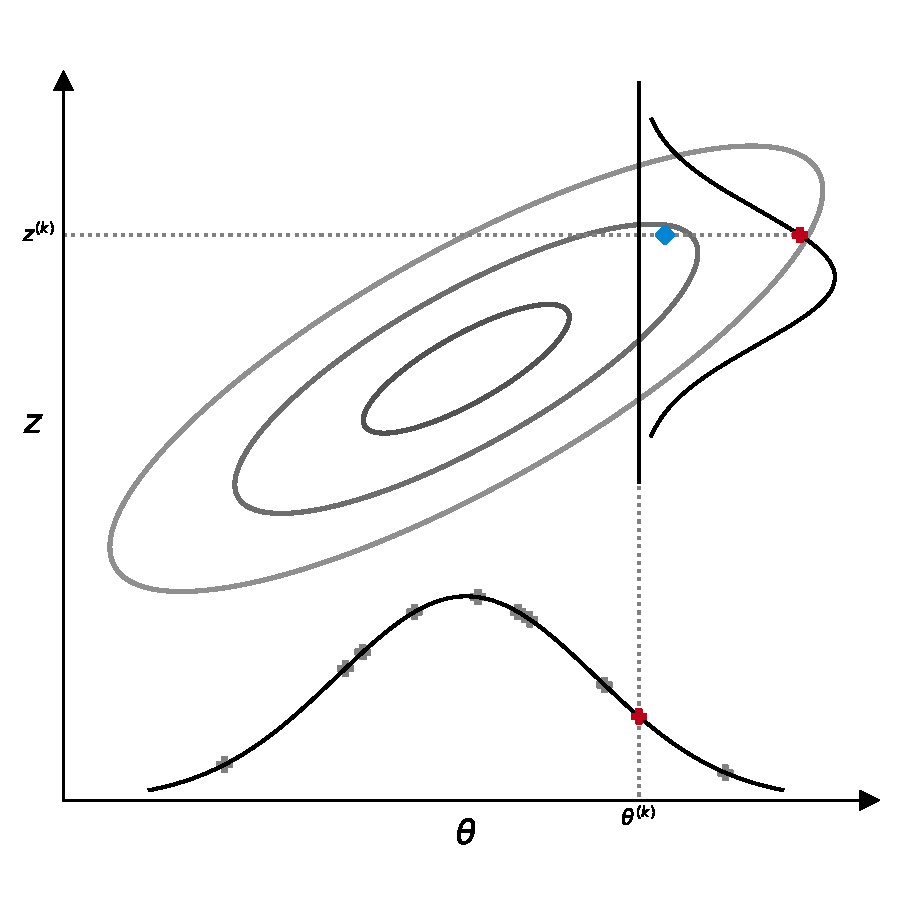
\includegraphics[width=3.25cm]{joint_dist_sampling.pdf}};

\node at (-3,-0.75) {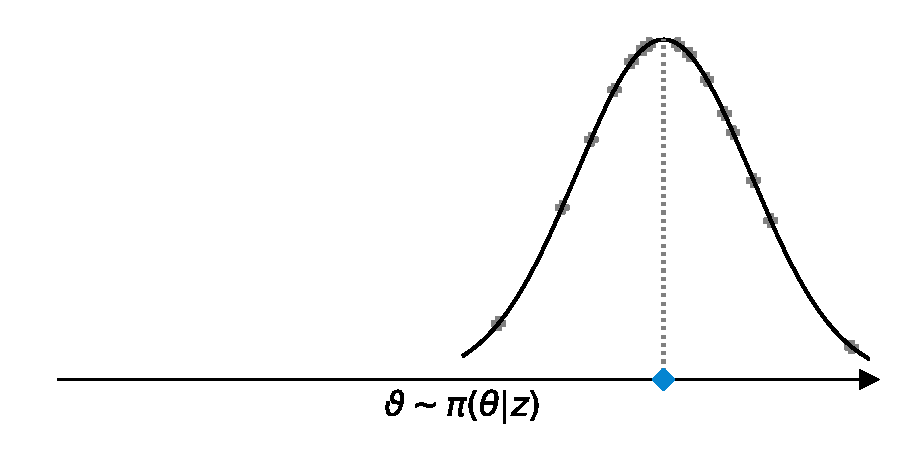
\includegraphics[width=2cm]{posterior_dist_sampling.pdf}};
\node at (-3,0.5) {\large Guess};

\begin{scope}
\clip (0,0) circle (1.25cm);
\node[circle, fill=white, minimum width=2.5cm] at (0,0) {};
\node (lp) at (0,0) {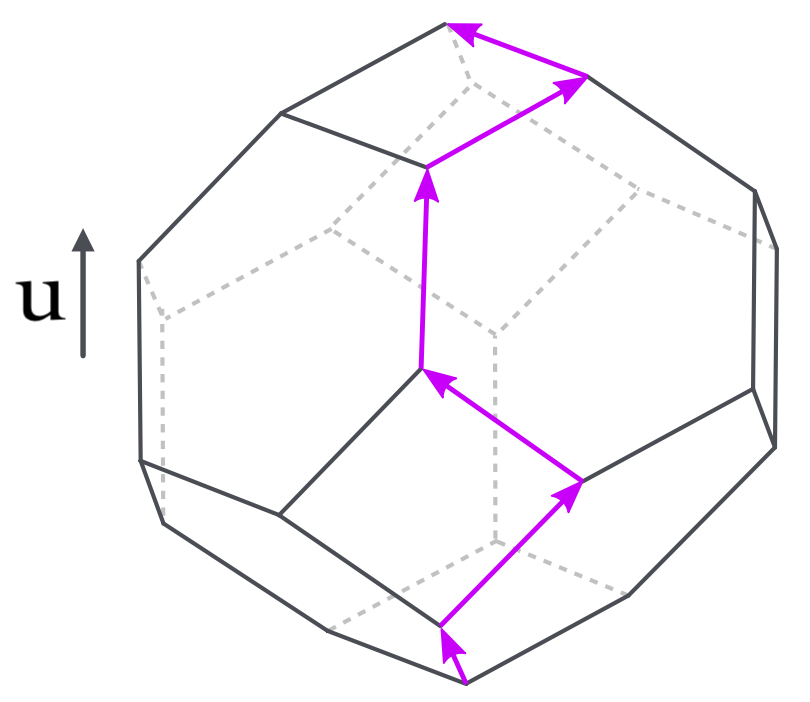
\includegraphics[width=2.3cm]{lp.png}};
\end{scope}

\node at (0, -1.65) {\large Decide};

\node at (2.6,0.5) {\large Imagine};

\node[rectangle, fill=white, minimum width=3.7cm, minimum height=1.9cm, rounded corners=7.5pt] (eval_bg) at (6,0) {};
\node (eval) at (6,0) {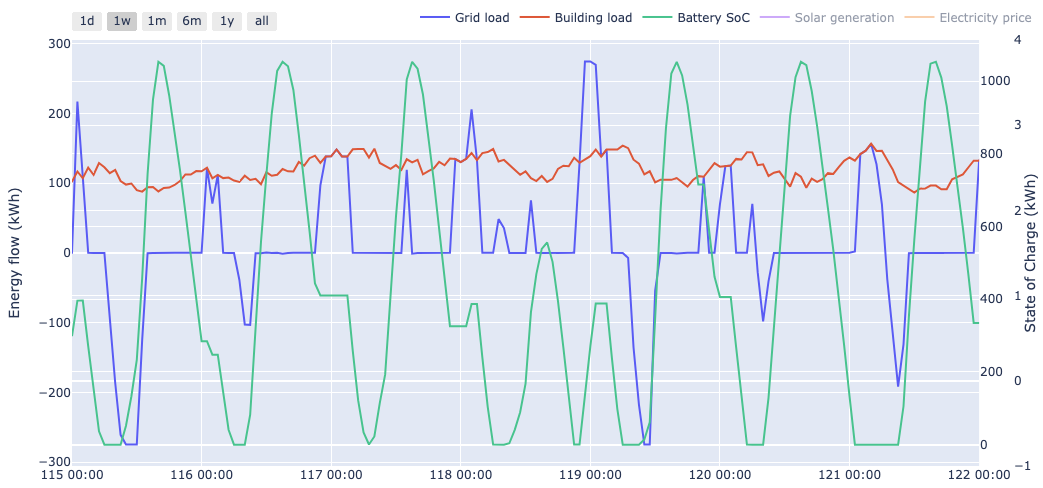
\includegraphics[width=3.5cm]{sim.png}};
\node[xshift=0.4cm, yshift=-0.45cm] (kpi) at (eval_bg.north west) {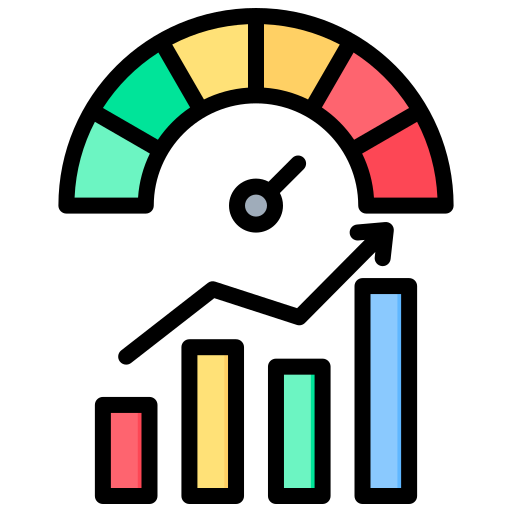
\includegraphics[width=0.65cm]{kpi.png}};

\node[align=right] at (4.8, -2.75) {\large Repeat};

\node[circle, fill=white, minimum width=1.25cm] (sigma) at (0,-3.25) {\HUGE $\mathlarger{\Sigma}$};

\begin{scope}[line width=.8mm, color=gray!75!black, arrows={-Stealth[inset=0pt, angle=60:10pt]}]
    \draw[shorten <= -2mm, shorten >= 1mm] (sample) -- (lp);
    \draw[shorten <= 1mm, shorten >= 1mm] (lp) -- (eval);
    \draw[shorten <= 1.5mm, shorten >= 1mm] (eval) |- (sigma);
    \draw[dashed, shorten <= 1mm, shorten >= -1.5mm] (sigma) -| (sample);
\end{scope}

\end{tikzpicture}
}
\end{cbox}

\vfill

% Brief intro to chapter explaining contents and flow.
\noindent
\glsxtrlong{voi} analysis (\glsxtrshort{voi}) is the main methodology used in this thesis to investigate the benefit of data collection for improving decision making. This chapter explains the \glsxtrlong{voi} framework. It begins with a brief introduction to \glsxtrshort{voi} and its history in \Cref{sec:methodology-intro}. The theory of the framework is then progressively built up through Sections \ref{sec:methodology-statistical-decision-theory} to \ref{sec:methodology-framework-extensions}. Alongside this theory, the interpretation of what the calculations are doing and their meaning is discussed, and a worked example of a simple building energy system is developed to illustrate how the results can inform decision making. Finally, the limitations of the framework are explored in Section \ref{sec:methodology-limitations}. % and practical considerations for computing \glsxtrshort{voi} values ... and \ref{sec:methodology-considerations}.

\newpage
%********************************** VoI intro section **************************************
\section{Introduction} \label{sec:methodology-intro}

% Nab from group VoI intro and other papers
% Explain the history of VoI, what it does (i.e. the question it answers), and where it has been used in the past (propose that it'd be extremely useful in the insurance industry)

\glsxtrlong{voi} analysis is a numerical framework for quantifying the expected benefit of collecting data to improve decision making by reducing uncertainty. The economic form was originally proposed by \citep{raiffa1961AppliedStatisticalDecision}\footnote{Though several other authors were working on similar ideas in other fields around the same time \citep{howard1966InformationValueTheory,hurley1964MathematicalTheoryValue,spivey1968DecisionMakingProbabilistic,feltham1968ValueInformation,szaniawski1967ValuePerfectInformation}}, and is built on Bayesian Decision Analysis and Expected Utility Theory \citep{smith1945TheoryGamesEconomic}. It investigates how reducing epistemic uncertainty in a system (uncertainty associated with a lack of knowledge of a system \citep{zhang2021ValueInformationAnalysis}) by taking measurements affects the average utility/performance of the decisions within that system. It numerically answers the question,

\begin{cbox}[colback=Aquamarine!10!white]{}
How much better on average would a decision maker do at a given problem by taking a measurement to reduce uncertainty before making their decision?
\end{cbox}
\vfill

\noindent
This question has been and remains extremely important in lots of disciplines, and \glsxtrshort{voi} has been used to study it in a wide variety of contexts. Early applications in the 1970s included \citep{conrad1980QuasiOptionValueExpected}, operations management \citep{bedford1966MeasuringValueInformation}, agriculture \citep{perrin1976ValueInformationValue}, accountancy \citep{mock1971ConceptsInformationValue}, wargaming \citep{oldham1996ValueInformation}, and hydrology \citep{klemes1977ValueInformationReservoir}. Due to the limited computational power available at the time, these studies used simple decision tree models of uncertainties and decision making. However, due to the interest in linear \glsxtrlong{sp} in Operations Research and Management Science at the time \citep{williams1965StochasticLinearProgramming,dantzig1955LinearProgrammingUncertainty,wilson1966ProgrammingUncertainty} following the success of \glsxtrlong{lp} in supply chain management \citep{dantzig1956RecentAdvancesLinear}, a few studies applied \glsxtrshort{voi} to decision making using small, early Linear Programs \citep{avriel1970ValueInformationStochastic}.

% Note: copied from VoI section of Lit Review
More recent uses include fields such as environmental science, medicine, agriculture, and economics \citep{keisler2014ValueInformationAnalysis}. For example in medicine, \glsxtrshort{voi} has been used to study the trade-off between reducing uncertainty in the efficacy of treatments and the cost of performing clinical trials \citep{willan2005ValueInformationOptimal}, and to decide whether further research is required before a new medical technology is adopted \citep{tuffaha2014ValueInformationAnalysis}.

Within engineering, \glsxtrshort{voi} has been used in contexts such as maintenance scheduling for buildings \citep{grussing2018OptimizedBuildingComponent} and wind farms \citep{myklebust2020ValueInformationAnalysis}, construction project planning \citep{esnaasharyesfahani2020PrioritizingPreprojectPlanning}, automotive design \citep{acar2009SystemReliabilityBased}, sensor placement \citep{malings2016ValueInformationSpatially}, and structural health monitoring \citep{difrancesco2021DecisiontheoreticInspectionPlanning,difrancesco2023SystemEffectsIdentifying}.

Review papers \citep{keisler2014ValueInformationAnalysis} and \citep{zhang2021ValueInformationAnalysis} provide thorough overviews of the applications of \glsxtrshort{voi} across disciplines and in engineering respectively.


%********************************** VoI theory section **************************************
\section{Statistical decision theory} \label{sec:methodology-statistical-decision-theory}

% Build up from the ground starting off with brief explanations of what we mean by optimization, expectations, etc., including notation

To understand how uncertainty affects decision making in a quantifiable way, we first need a mathematical framework for making decisions. For this we'll use the mathematics of optimisation\footnote{In the energy systems field this is referred to as optimisation based design/control \citep{barber2022ReviewOptimizationBased}}. Numerical optimisation provides us with a well-defined, objective, and consistent way to make decisions, which does not rely on unquantifiable human judgement\footnote{Of course the setup of our optimisation \textit{is} determined by subjective human judgement. We need to define what we care about, i.e. what objective we want to optimise and what our constraints are. We can never really achieve complete objectivity. But, given a particular problem we want to solve, with a goal we can quantify, optimisation give us an objective tool for tackling it.}.\\

Let's imagine we have some problem we want to solve\footnote{We are the decision maker, also called the `actor'.}, and to do so we have to select one choice, which we'll call an `action' $a$, from a set of possible actions, $\mathcal{A}$. How well each action does at our problem is described by a utility function, $u(a)$. Our actions can have multiple aspects (or dimensions), and the utility function returns a single number for each action which describes how `good' it is at solving the problem. % For example, ...
Costs can be described with negative utilities.

We want to find the best action to take, that is the one which achieves the highest utility. Mathematically we describe this optimisation problem\footnote{Mathematics uses somewhat different notation from decision theory to describe optimisation problems, see \citep{boyd2004ConvexOptimization}.} as,
\begin{equation}
    \mathlarger{\max_{a \in \mathcal{A}} \: u(a)}
\end{equation}
How to actually search through the set of possible actions to find the optimal choice for a practical problem is a complicated question. There are many \textit{many} different optimisation algorithms, all of which are suited to different situations \citep{bonnans2006NumericalOptimizationTheoretical}. But for our purposes, let's assume we can choose a suitable method for our problem, and that we are able to properly optimise our utility to find the best action, which is the one we'll take.\\

This is a simple deterministic model of decision making which assumes we know exactly how the action we take will perform. However in practical engineering systems, there are usually factors which we don't precisely know at the time the decision is made that affect how the different actions will perform when taken, i.e. the utility they achieve. Because of these uncertain factors, which we'll refer to as the `uncertainties' of the system, $\theta$, there are many possible outcomes if a given action is taken. We can graphically represent this process of taking an action, realising the value of the uncertainties, and observing an outcome/utility, using a decision tree which is illustrated in \Cref{fig:methodology-DT-prior}.

\begin{figure}[h]
    \vspace*{-1.5cm}
    {\centering
    \begin{tikzpicture}[node distance=0cm]

    % Nodes
    \node[DTnode, rectangle] (action) at (0,0) {$A$};
    \node[annot, below of=action, yshift=-\tkzlabsep] {$a \in \mathcal{A}$};
    \node[DTnode, circle, right of=action, xshift=\tkzhsep, yshift=\tkznodeysep] (theta) {$\theta$};
    \node[annot, below of=theta, yshift=-\tkzlabsep] {$\theta \sim \pi(\theta)$};
    \node[DTnode, triangle, right of=theta, xshift=\tkzhsep, yshift=-\tkznodeysep] (utility) {$U$};
    \node[annot, below of=utility, yshift=-\tkzlabsep] {$u\left(a,\theta\right)$};

    % True arcs
    \begin{scope}[ultra thick]
        \draw[->] (action) -- (theta);
        \draw[->, dashed] (theta) -- (utility);
    \end{scope}

    % Dummy nodes
    \node[DTnode, dummy, circle, draw=none, below of=theta, yshift=2*\tkznodeysep]  (dt1) {};
    \node[DTnode, dummy, circle, draw=none, below of=theta, yshift=-2*\tkznodeysep]  (dt2) {};
    \node[DTnode, dummy, circle, draw=none, below of=theta, yshift=-4*\tkznodeysep]  (dt3) {};

    \node[DTnode, dummy, circle, draw=none, below of=utility, yshift=4*\tkznodeysep]  (du1) {};
    \node[DTnode, dummy, circle, draw=none, below of=utility, yshift=2*\tkznodeysep]  (du2) {};
    \node[DTnode, dummy, circle, draw=none, below of=utility, yshift=-2*\tkznodeysep]  (du3) {};

    % Dummy arcs
    \begin{scope}[draw=gray]
        \draw[-] (action) -- (dt1);
        \draw[-] (action) -- (dt2);
        \draw[-] (action) -- (dt3);
        \draw[-] (theta) -- (du1);
        \draw[-] (theta) -- (du2);
        \draw[-] (theta) -- (du3);
    \end{scope}

    \end{tikzpicture}
    \vspace*{-1.5cm}
    \caption{Decision tree representation of decision making under uncertainty.} \label{fig:methodology-DT-prior}
    \vspace*{0.15cm}
    {\hfill
    \footnotesize{Adapted from Figure 1 of \citep{difrancesco2021DecisiontheoreticInspectionPlanning}}
    \hfill}
    }
\end{figure}

While we don't know the value of the uncertainties, and so the outcome that we'll get, we typically do have probabilistic knowledge of them. This knowledge comes in the form of their probabilistic model or distribution\footnote{In this chapter will assume that you are somewhat familiar with probabilities, likelihoods, sampling from distributions, and calculating expectations. If not, there are many textbooks and courses that introduce these statistical ideas, such as \citep{schwarzlander2011ProbabilityConceptsTheory}.}\fnsep\footnote{The distributions of the uncertainties can either be modelled using existing data from similar system, or by making reasonable assumptions based off knowledge of the system. The choice of these distributions is a critical modelling step \citep{vandeschoot2021BayesianStatisticsModelling}.}, $\pi(\theta)$.

As the utility now depends on both the action and the value of the uncertainties, $u(a,\theta)$, there is now also uncertainty or risk associated with the utility we'll get, which we must manage during decision making. There are many ways of handling this risk, such as taking the action with the `best worst-case' utility, or the one with the best robustness guarantees. But the most common way is to take the action with the highest average (or expected) utility\footnote{The framework can be easily adapted to use whichever uncertainty management method is most appropriate for the decision making context. This is done by simply changing the objective. For example in \Cref{chap:parks}, a \glsxtrlong{cvar} term is added to the objective to incorporate risk aversion into the decision making. In fact, many risk management methods just adjust the utility function, adding a risk term, and still optimise the expectation.}. So the `objective' we now want to optimise to determine our action choice is the expected value of the utility over the uncertainties in the system,
\begin{equation} \label{eq:methodology-prior-optimisation}
    \mathlarger{\max_{a \in \mathcal{A}} \: \mathbb{E}_{\theta}\lbrace u(a,\theta) \rbrace}
\end{equation}

\newpage

\noindent
However, for real engineering problems we typically cannot calculate this expectation exactly\footnote{The expectation can only be calculated exactly if the probabilistic model of the uncertainties used is discrete, or if the utility function is very simple.}. Instead, we use a \glsxtrlong{mc} (\glsxtrshort{mc}) estimate to approximate it\footnote{In this thesis, whenever there is an expectation, we will use an \glsxtrshort{mc} estimate of it in our numerical calculations.}. To do so, we draw a number of samples from the distributions of the uncertainties, $\theta^{(n)} \sim \pi(\theta)$, and compute the average utility over those samples,
\begin{equation}
    \mathlarger{\frac{1}{N} \sum_n u\big(a,\theta^{(n)}\big)}
\end{equation}
As the number of samples used, $N$, increases, this approximation improves, and the estimate converges to the true value of the expectation.

So to solve our decision making problem under uncertainty, we optimise the average utility achieved over the sampled values of the uncertainties,
\begin{equation}
    \mathlarger{\max_{a \in \mathcal{A}} \: \mathbb{E}_{\theta}\lbrace u(a,\theta) \rbrace \: \approx \: \max_{a \in \mathcal{A}} \: \frac{1}{N} \sum_n u\big(a,\theta^{(n)}\big)}
\end{equation}
Doing so tells us the best action to take, $a^*$, and how `good' we expect it to be at solving our problem, i.e. the average utility it achieves. We can also use the distribution of its utility over the uncertainty samples to understand the risk associated with our decision making.\\

More generally, this type of optimisation is referred to as a `stochastic decision problem'. It is fully specified by the set of possible actions, $\mathcal{A}$, the probabilistic model of uncertainties, $\pi(\theta)$, and the utility function\footnote{Strictly, it's the optimisation objective which is a function of the utility that defines the problem, but these are often used interchangeably.}, $u(a,\theta)$. Solving the stochastic optimisation in Eq. \ref{eq:methodology-prior-optimisation} gives us the best solution to this problem. But solving it can be very computationally expensive, as the utility function needs to be evaluated $N$ times due to the sampling\footnote{In fact for a Stochastic Program, the computational cost of using this average utility scales as $\mathcal{O}(N^3)$.}. Instead, we could try to solve the problem using some heuristic \citep{pickering2016ComparisonMetaheuristicLinear}. A common approach is to use the expected (average) values of the uncertainties in a deterministic optimisation, which is called the \glsxtrlong{evp} (\glsxtrshort{evp}). This is a much cheaper problem to solve, but may not correctly identify the best action to take. The difference in expected utilities achieved by the stochastic optimisation (Eq. \ref{eq:methodology-prior-optimisation}) and the solution to the \glsxtrshort{evp} tells us how much better we can do at solving the decision problem by accounting for the uncertainties in the system in our optimisation, and is referred to as the \glsxtrlong{vss} (\glsxtrshort{vss}) \citep{bistline2015ElectricSectorCapacity}. Actually, we could use whatever policy\footnote{The term `policy' is used to refer to any structured way of making decisions. E.g. a flow chart defines a policy.} we like to try to solve the decision problem. This more general setting is discussed in \Cref{sec:methodology-on-policy-voi}.

\newpage

\begin{ebox}[label=ebox:opt]{Introducing an example problem}
    To help clarify this discussion of mathematics and understand why it's useful to us, let's apply it to something concrete and introduce an example problem. We'll developed this example problem throughout the chapter, and demonstrate how we can use each step of the mathematical framework as we introduce it. Code for all the calculations in this example is available for you to try out and explore at \url{https://github.com/mal84emma/VoI-Tutorial}.

    \subsubsection*{Designing a solar-battery system for a commercial building}
    \vspace*{-1ex}
    Let's imagine we want to decarbonise the energy use of a hypothetical commercial building. To do this we plan to install solar panels and battery storage in the building. This equipment is expensive, but by generating our own energy and doing some energy trading with the grid we can reduce the electricity bill. So our goal is to design the solar-battery system for the building, that is choose the sizing of solar panels and battery storage, to minimise the total cost of meeting the building's energy demands.

    To help make this design decision we'll use a simple model of the building energy system to calculate the overall cost of constructing and operating the system, which is described in Appendix \ref{app:example-problem-formulation}.\\

    Initially, we'll optimise the system design by looking at 5 design options selected using our experience of building energy systems, and run the energy model to identify the design with the lowest cost. These design options are chosen to generate between 66\% and 100\% of the building's annual energy demand with the solar panels, and to use between a 4hr and 8hr battery to capture and shift the solar peak. The cost of each design is determined by running the model simulation using data from a single design year, in this case 2017. We can compare these costs in \Cref{tab:example-det-optimisation-results}.\\
    % \footnote{The solar capacity factor in Cambridge is roughly 0.13, meaning generating the energy demand over the year (which is 100kW on average) requires roughly 750kW of solar panels.}

    The results show us that there is a trade-off between the capital and operating costs, and that the design with 750kW of solar panels and 600kWh of battery storage gives us the best balance. With this design, it costs us £152.3k/yr in total to supply the building load, equivalent to £0.174/kWh. If the solar-battery system wasn't installed, buying all the electricity from the grid would cost £219.2k/yr (or £0.250/kWh), so we save £66.9k/yr (a 31\% cost reduction) by installing the system, as well as significantly reducing our carbon emissions.

    {\centering
    \renewcommand{\arraystretch}{0.8}
    \begin{tabularx}{0.975\linewidth}{ccccc}
        \toprule \toprule
        \makecell{Solar capacity\\(kWp)} & \makecell{Battery capacity\\(kWh)} & \makecell{Capital cost\\(£k/yr)} & \makecell{Operating cost\\(£k/yr)} & \makecell{Annualised\\cost (£k/yr)} \\
        \midrule \midrule
        \multicolumn{5}{>{\centering\arraybackslash}l}{\small \textit{Discrete design options} \hspace{6.9cm} (Discrete optimisation)} \\[0.5ex]
        500 & 400 & 65.5 & 100.6 & 166.1 \\
        500 & 600 & 79.5 & 91.4 & 170.9 \\
        600 & 600 & 87.0 & 76.1 & 163.1 \\
        \textbf{750} & \textbf{600} & 98.2 & 54.1 & \textbf{152.3} \\
        750 & 800 & 112.2 & 46.3 & 158.6 \\
        \midrule
        \multicolumn{5}{>{\centering\arraybackslash}l}{\small \textit{Linear Program solution} \hspace{6.25cm} (Continuous optimisation)} \\[0.5ex]
        889 & 501 & 101.7 & 39.3 & \textbf{141.0} \\
        \bottomrule \bottomrule
    \end{tabularx}
    \bigskip
    \captionof{table}{Deterministic design optimisation results.} \label{tab:example-det-optimisation-results}
    }\

    We have in some sense optimised this system design, but we've only looked through a very small number of options. We could search through lots more options, but this would be very computationally expensive. However, our building energy system model actually uses a Linear Program (\glsxtrshort{lp}) to optimise the operation of the system and find lowest cost of running it. So, we can include the solar and battery capacities as decision variables in our \glsxtrshort{lp} optimisation, and use the nice mathematics of our model to find the best capacities out of all possible options, and so the `optimal' design. This solution is also shown in \Cref{tab:example-det-optimisation-results}. Using the  \glsxtrshort{lp} leads us to a design we might not have chosen to explore. It generates more solar energy than the building can use, and is more cautious with the batteries than we were. And importantly, it reduces the cost by 7.4\% compared to our best design guess.\\

    This design optimisation is all well and good, but we've completely neglected the fact that there are many factors that will affect the operation, and so cost of running of our energy system, that we don't know at the time we design it. So let's introduce some uncertainties into our model, and see how they affect our design decisions. We'll account for uncertainties in the building load, solar generation, and the cost and efficiency of the battery storage. The probabilistic models we'll use are described in Appendix \ref{app:example-problem-uncertainties}.

    We can repeat the optimisations from before, but now we will draw 50 samples\footnote{This isn't that many samples, and so our estimate of the expected cost might have some noisy/inaccurate, but this is the largest number we can use within an achievable computational cost.} from the distributions of the uncertainties, and our design objective will be the average cost from the energy model over these samples. We call a set of values sampled from the uncertainties a `scenario'.

    {\centering
    \renewcommand{\arraystretch}{0.8}
    \begin{tabularx}{0.975\linewidth}{ccccc}
        \toprule \toprule
        \makecell{Solar capacity\\(kWp)} & \makecell{Battery capacity\\(kWh)} & \makecell{Av. capital\\cost (£k/yr)} & \makecell{Av. operating\\cost (£k/yr)} & \makecell{Av. annualised\\cost (£k/yr)} \\
        \midrule \midrule
        \multicolumn{5}{>{\centering\arraybackslash}l}{\small \textit{Discrete design options} \hspace{6.9cm} (Discrete optimisation)} \\[0.5ex]
        500 & 400 & 65.5 & 95.7 & 161.2 \\
        500 & 600 & 79.6 & 86.4 & 166.0 \\
        600 & 600 & 87.1 & 71.1 & 158.1 \\
        \textbf{750} & \textbf{600} & 98.3 & 49.1 & \textbf{147.4} \\
        750 & 800 & 112.3 & 41.2 & 153.6 \\
        \midrule
        \multicolumn{5}{>{\centering\arraybackslash}l}{\small \textit{Stochastic Program solution} \hspace{5.6cm} (Continuous optimisation)} \\[0.5ex]
        807 & 429 & 90.5 & 49.4 & \textbf{139.9} \\
        \bottomrule \bottomrule
    \end{tabularx}
    \bigskip
    \captionof{table}{Stochastic design optimisation results.} \label{tab:example-stoch-optimisation-results}
    }\

    Comparing to the results from \Cref{tab:example-det-optimisation-results} for the discrete optimisation, we can see that the same design option is selected as before, but that there is a about a 3\% difference in the estimated cost of the system. I.e. using the single design year causes us to overestimate the cost of the system compared to the actual average.

    Designing using the \glsxtrshort{lp}, which is now a Stochastic Program\footnote{Specifically, it's a linear scenario program, where the (linear) operating constraints of each scenario are all included in the model, and the objective is the average total cost over the scenarios. See Eq. \ref{eq:example-problem-formulation}.} (\glsxtrshort{sp}), leads to a design which uses around 10\% smaller capacities than the deterministic case, but doesn't cause a significant change in total cost between the designs\footnote{Unfortunately we cannot actually compute the \glsxtrshort{vss} as the deterministic LP solution is infeasible, which is a problem, but we can approximate it. This issue is discussed further in Appendix \ref{app:methodology-constraints-tirade}.}.

    So in this case, accounting for these pretty significant uncertainties in our optimisation model doesn't have a substantial impact on the design decision\footnote{Though this might depend on the design year we chose. We may have just got lucky.}, but it does provide us with a better estimate of how much the system might cost\footnote{Not only is the average cost value more accurate, but the statistical information about the possible costs is also useful for planning.}.

    Another advantage of accounting for uncertainties in our design model is that we also get information about the resulting uncertainty in the cost, which can be useful for planning and managing risk.
    Over the 50 scenarios, the total cost of the 750kWp--600kWh system varied from £110.4k/yr to £175.5k/yr, with a standard deviation of £16.6k/yr.
    Knowing that the cost could get this high would be important if we had a strict budget constraint, and might cause us to choose a different design\footnote{If we were very risk averse, we might want to optimise for the maximum cost, rather than the average.}. Or ask for a bigger budget.
\end{ebox}

\newpage
\section{Bayesian decision analysis} \label{sec:methodology-bayesian-decision-analysis}

% Explain what the inclusion of measurements does, how Bayes is applied, and how the framework operates - we now give the decision maker the option to collect data before taking a decision action, which will inform them about the uncertainties and improve their decision making ability

While we are able to manage uncertainties during our decision making, their presence is problematic for decision making. This is because when we are hedging our decision to perform well on average, we're missing out on making the best decision for the state of the system that we'll actually get (the true values of the uncertainties). Though of course at the time we are making our decision we don't know what that will be. But, if we were able to reduce the uncertainty in our problem\footnote{Not all uncertainties can be reduced. There are two types of uncertainty. Aleatoric uncertainty, which is inherent variability which cannot be explained away, and epistemic uncertainty, which is uncertainty associated with a lack of knowledge of the system, which can be reduced through data collection. Often in engineering systems uncertain parameters have a mix of aleatoric and epistemic, meaning their uncertainty can be reduced but never fully removed.\label{fn:aleatoric}}, and get better information about the true state of the system, we would need to hedge less, and so could do a better job of making our decision.

Let's consider how our decision making will change if we are able to take a measurement/collect data that reduces the uncertainties before we have to make our decision.\\

First of all we need to be able to describe how the data informs us of the true state of the system and reduces the uncertainties. We do this using a likelihood function. For a measurement, $e$, the likelihood function, $f_e(z|\theta)$, describes the chance of getting a particular value/data from the measurement, $z$, if the true value of the uncertainties is $\theta$. This is to say it describes the uncertainty associated with the measurement\footnote{A standard likelihood function is a Normal/Gaussian with a precision/variance that is determined from lab experiments, e.g. $\pm10\%$ meaning the standard deviation would be 5\% of the mean (for a 95\% confidence level).}.

Bayes' theorem tells us the following,
\begin{equation}
    p(\theta \mid z) = \frac{p(z \mid \theta) \: p(\theta)}{p(z)} \propto p(z \mid \theta) \: p(\theta)
\end{equation}
where $p(\theta)$ is the prior distribution of the uncertainties, $p(z \mid \theta)$ is the likelihood function of the measurement, and $p(\theta \mid z)$ is the posterior distribution of the uncertainties for a given measurement value/data $z$.

The prior distribution describes our initial knowledge of the uncertainties. The likelihood function describes the knowledge/information we gain from the data. And the posterior distribution combines these two pieces of information, and tells us about the remaining uncertainty given what we've observed.\\

Though the framework is typically described in terms of physical measurements, we can apply these ideas to any source of information that reduces the uncertainty in our problem, such as research, improved forecasting methods, or getting expert advice. The only requirement is that we can model the uncertainty reduction that information provides\footnote{Though if modelling this uncertainty reduction is tricky, we can make a best guess and use sensitivity analysis to see if that guess affects our conclusions.}, i.e. come up with a likelihood function.

As the \glsxtrshort{voi} framework is numerical, we can use a probabilistic programming language such as \href{https://mc-stan.org/}{\texttt{Stan}} \citep{carpenter2017StanProbabilisticProgramming} to sample from the required distributions, giving lots of flexibility in how we can model the uncertainties and how they are reduced by data collection.\\

At the time we're considering whether to take a measurement to support our decision making, we can't know what value/data, $z$, we'll get from the measurement. This means there are many possible outcomes for each available measurement option. Once we've received the data from our measurement, we can use it to form a posterior distribution of the uncertainties, $\pi(\theta|z)$, which has reduced uncertainty compared to the initial, prior distribution. We use this improved information to support and improve our decision making, performing the same stochastic decision process as before, but now using the updated knowledge of the possible outcomes of our actions. We can represent this extra measurement step in the decision making process by extending the decision tree, as shown in \Cref{fig:methodology-DT-prepost}.

\begin{figure}[h]
    \vspace*{-1.5cm}
    {\centering
    \begin{tikzpicture}[node distance=0cm]
    
    % Nodes
    \node[DTnode, rectangle] (measure) at (0,0) {$E$};
    \node[annot, below of=measure, yshift=-\tkzlabsep] {$e \in E$};
    \node[DTnode, circle, right of=measure, xshift=\tkzhsep, yshift=\tkznodeysep] (z) {$Z$};
    \node[annot, below of=z, yshift=-\tkzlabsep] {$z \sim \pi(z)$};
    \node[DTnode, rectangle, right of=z, xshift=\tkzhsep, yshift=-\tkznodeysep] (action) {$A$};
    \node[annot, below of=action, yshift=-\tkzlabsep] {$a \in \mathcal{A}$};
    \node[DTnode, circle, right of=action, xshift=\tkzhsep, yshift=\tkznodeysep] (theta) {$\theta$};
    \node[annot, below of=theta, yshift=-\tkzlabsep] {$\theta \sim \pi(\theta | z)$};
    \node[DTnode, triangle, right of=theta, xshift=\tkzhsep, yshift=-\tkznodeysep] (utility) {$U$};
    \node[annot, below of=utility, yshift=-\tkzlabsep] {$u\left(a,\theta\right)$};

    % True arcs
    \begin{scope}[ultra thick]
        \draw[->] (measure) -- (z);
        \draw[->, dashed] (z) -- (action);
        \draw[->] (action) -- (theta);
        \draw[->, dashed] (theta) -- (utility);
    \end{scope}
    
    % Dummy nodes
    \node[DTnode, dummy, circle, draw=none, below of=z, yshift=2*\tkznodeysep]  (dz1) {};
    \node[DTnode, dummy, circle, draw=none, below of=z, yshift=-2*\tkznodeysep]  (dz2) {};
    \node[DTnode, dummy, circle, draw=none, below of=z, yshift=-4*\tkznodeysep]  (dz3) {};

    \node[DTnode, dummy, circle, draw=none, below of=action, yshift=4*\tkznodeysep]  (da1) {};
    \node[DTnode, dummy, circle, draw=none, below of=action, yshift=2*\tkznodeysep]  (da2) {};
    \node[DTnode, dummy, circle, draw=none, below of=action, yshift=-2*\tkznodeysep]  (da3) {};

    \node[DTnode, dummy, circle, draw=none, below of=theta, yshift=2*\tkznodeysep]  (dt1) {};
    \node[DTnode, dummy, circle, draw=none, below of=theta, yshift=-2*\tkznodeysep]  (dt2) {};
    \node[DTnode, dummy, circle, draw=none, below of=theta, yshift=-4*\tkznodeysep]  (dt3) {};

    \node[DTnode, dummy, circle, draw=none, below of=utility, yshift=4*\tkznodeysep]  (du1) {};
    \node[DTnode, dummy, circle, draw=none, below of=utility, yshift=2*\tkznodeysep]  (du2) {};
    \node[DTnode, dummy, circle, draw=none, below of=utility, yshift=-2*\tkznodeysep]  (du3) {};
    
    % Dummy arcs
    \begin{scope}[draw=gray]
        \draw[-] (measure) -- (dz1);
        \draw[-] (measure) -- (dz2);
        \draw[-] (measure) -- (dz3);
        
        \draw[-] (z) -- (da1);
        \draw[-] (z) -- (da2);
        \draw[-] (z) -- (da3);

        \draw[-] (action) -- (dt1);
        \draw[-] (action) -- (dt2);
        \draw[-] (action) -- (dt3);

        \draw[-] (theta) -- (du1);
        \draw[-] (theta) -- (du2);
        \draw[-] (theta) -- (du3);
    \end{scope}
    
    \end{tikzpicture}
    \vspace*{-1.5cm}
    \caption{Decision tree representation of decision making with measurements} \label{fig:methodology-DT-prepost}
    \vspace*{0.15cm}
    {\hfill
    \footnotesize{Adapted from Figure 1 of \citep{difrancesco2021DecisiontheoreticInspectionPlanning}}
    \hfill}
    }
\end{figure}\

While these decision trees illustrate the sequence of our decision making, the available choices and their possible outcomes, they are only really useful for illustrating simple toy problems. For complex, real world decision making problems, we use influence diagrams to provide a clear and concise visual description of the structure of the system and decision making. These diagrams show only the causal dependencies between decisions, uncertainties, and outcomes in the system, and allow domain experts to quickly describe decision making in complex engineering systems. They are excellently explained by \citep{difrancesco2023GuidanceUseProbabilistic}.\\
% \footnote{... from computational perspective, uncertainties are sampled, and passed as inputs to simulators for variables, which are then inputs to utility calculation ...}

To understand how collecting this data affects our decision making, we can update our decision optimisation to use this improved information that reduces the uncertainties in the problem,
\begin{equation} \label{eq:methodology-posterior-optimisation}
    \mathlarger{\max_{a \in \mathcal{A}} \: \mathbb{E}_{\vartheta|z}\lbrace u(a,\vartheta) \rbrace}
\end{equation}
This new optimisation (stochastic decision problem) can be used to find the decision we would make if we'd received data $z$. We refer to this as the Posterior decision problem, as we are now finding the action that performs best on average under the remaining uncertainty given by the posterior distribution, $\pi(\theta|z)$\footnote{Note, in Eq. \ref{eq:methodology-posterior-optimisation} we use $\vartheta$ to denote estimates of the true value of the uncertainties which are made after data $z$ is received, to differentiate from the possible true values of the uncertainties $\theta$ that we will later average over.}.\\

However, because we don't know what data $z$ we'll receive before we measure, to understand how well we would do using data to support our decision making, we need to average over the possible values of the measurement data\footnote{We also explicitly average over the possible values of the uncertainties, $\theta$, as the measurement values are associated with the true states of the system. During sampling, we first sample $\theta$ values from the prior, and then sample the corresponding likelihood function to obtain $z$ values.},
\begin{equation} \label{eq:methodology-preposterior-value}
    \mathlarger{ \mathbb{E}_{\theta,z} \left\lbrace \max_{a \in \mathcal{A}} \: \mathbb{E}_{\vartheta|z}\lbrace u(a,\vartheta) \rbrace \right\rbrace}
\end{equation}
This tells us how well we would do on average at solving our decision problem, i.e. the expected utility we'd achieve, if we were to gather data to reduce the uncertainties in the problem before making our decision.

We refer to this as the Pre-Posterior decision problem, as we are averaging over all of the possible Posterior decision problems corresponding to each measurement value $z$. Eq. \ref{eq:methodology-prior-optimisation} from before is referred to as the Prior decision problem, as there our decisions are made with only the information from the prior distribution, $\pi(\theta)$.\\

When solving the Pre-Posterior decision problem numerically, we first hypothesis possible values $z$ we could receive from the measurement by sampling from the prior and likelihood functions. Then, for each sampled $z$ value, we consider what the corresponding Posterior decision problem with reduced uncertainty would be, how we would solve it, and how well we would do. Finally, we average those expected utilities to estimate the overall expected utility over solving the decision problem with the help of data collection.

\begin{equation}
    \mathlarger{
        \frac{1}{N} \mathlarger{\sum}_{z^{(n)} \sim f_e(z|\theta^{(n)})} \max_{a \in \mathcal{A}} \Bigg( \frac{1}{M} \mathlarger{\sum}_{\vartheta^{(m)} \sim \pi(\vartheta|z^{(n)})} u\big(a,\vartheta^{(m)}\big) \Bigg)
    }
\end{equation}
\smallskip

\noindent
This means we now get a distribution of the actions we would take given the possible measured values, and how well we would do at solving our problem in each case.\\

Collecting data to reduce the uncertainty in the problem will improve our decision making ability. This is because the decisions we now make are more tailored to the actual state of the system (which we now know more precisely) and use less hedging. We could always take the decision we would initially have made (i.e. our choice from the prior decision problem), but if we see certain data values we can adjust our decision to take a choice better suited to the likely state of the system. We can demonstrate this improvement from uncertainty reduction mathematically,
\begin{equation} \label{eq:methodology-pdp-inequality}
    \mathbb{E}_{\theta,z} \left\lbrace \max_{a \in \mathcal{A}} \: \mathbb{E}_{\vartheta|z}\lbrace u(a,\vartheta) \rbrace \right\rbrace
    >
    \max_{a \in \mathcal{A}} \: \mathbb{E}_{\theta,z} \left\lbrace \mathbb{E}_{\vartheta|z}\lbrace u(a,\vartheta) \rbrace \right\rbrace
    =
    \max_{a \in \mathcal{A}} \: \mathbb{E}_{\theta} \left\lbrace u(a,\theta) \right\rbrace
\end{equation}
\hspace{1.5em}

In the more general case where we have a set of measurement options, $E$, are available to take, we can also optimise our choice of measurement,
\begin{equation} \label{eq:methodology-preposterior-optimisation}
    \mathlarger{
    \max_{e \in E} \: \mathbb{E}_{\theta,z} \left\lbrace \max_{a \in \mathcal{A}} \: \mathbb{E}_{\vartheta|z}\lbrace u(a,\vartheta) \rbrace \right\rbrace
    }
\end{equation}
\hfill \\

\begin{ebox}[label=ebox:bayes]{Measuring building energy usage}
    % Provide probabilistic models (including example of uncertainty reduction from measurement - discuss both perfect and imperfect measurements, and why perfect is unrealistic) and influence diagram for the example problem (explain what nodes and arrows mean)
    % ? Explain how the decision making process would proceed with the measurement included, and discuss how we optimise over the posterior expectation now (same from this new, updated distribution) - kind of already done this, but contextualise
    % Provide the distribution of designs for each hypothesised measurement value (maybe show the utility dist - perhaps with point colour), leave expected utility for VoI part

    Previously in our example problem, we acknowledged that when we design the solar-battery system, we don't know exactly the amount of energy the building will use during operation. And we accounted for this uncertainty in the building load in our design decision, as well as other uncertainties, finding the design that provides the lowest cost on average.

    Our hypothetical commercial building has a design load of 100kW, and from our experience of previous buildings, we expect that the load during operation will be within $\pm20\%$ of this value. So we modelled this uncertain load using a Normal distribution truncated at 2 standard deviations,
    \begin{equation*}
        \theta_{\text{load}} \sim TN(\mu=100, \sigma=10, a=80, b=120)
    \end{equation*}
    This distribution of the load uncertainty, the prior distribution, describes our initial knowledge of the building load, also called our prior knowledge/belief.\\

    We can reduce this load uncertainty by gathering data from the building. For example by collecting monthly energy usage data from the building's electricity meter. Again from our experience of other buildings, we know that the energy usage of a building in future years is likely to be within $\pm5\%$ of the previous year's usage\footnote{Assuming there are no significant changes to the building, e.g. changes of usage or retrofits. At the time of designing the solar-battery system we do not expect any such changes, as heat pumps have recently been installed to decarbonise the building's heating.}.
    So we can describe the information we'd get from this metering data using the following likelihood function,
    \begin{equation*}
        z_{\text{load}}|\theta_{\text{load}} \sim \mathcal{N}(\mu=\theta_{\text{load}}, \sigma=\varepsilon\,\theta_{\text{load}})
    \end{equation*}
    where $\theta_{\text{load}}$ is the uncertain operational building load, $z_{\text{load}}$ is the previous year's load we get from the metering data and use to estimate future loads, and $\varepsilon=0.025$\footnote{To put our experience of future years' energy usage being within $\pm5\%$ of the previous year's within a $95\%$ confidence interval.}.\\

    The uncertainty reduction that collecting this metering data provides is illustrated in Fig. \ref{fig:methodology-example-load-uncertainty-reduction}, which shows the prior distribution of the building load during operation, an example annual load value (measurement) we might get from the electricity meter, and the corresponding posterior distribution.\\

    {
        \centering
        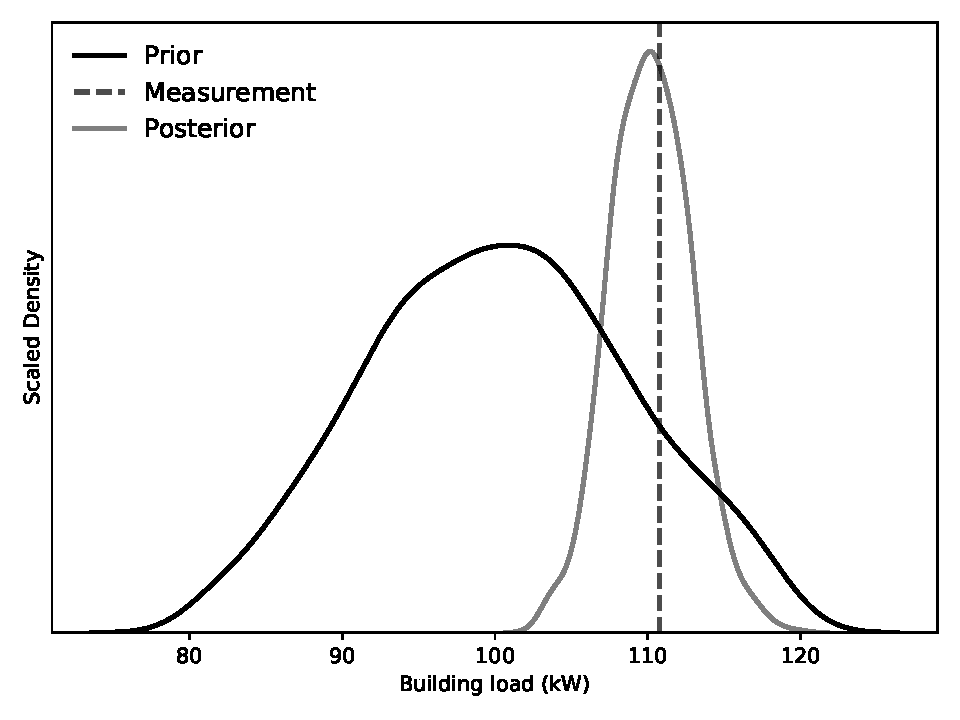
\includegraphics[width=0.66\linewidth]{Methodology/Figs/msr_uncertainty_reduction.pdf}
        \vspace*{-0.25cm}
        \captionof{figure}{Example reduction in load uncertainty provided by metering data.}
        \label{fig:methodology-example-load-uncertainty-reduction}
    }
    \smallskip

    % Think about design decisions with this metering data. Here's the influence diagram ...
    Reducing uncertainty in the building load gives us a better understanding of whether energy we generate with the solar panels can be used by the building, and how much energy we need to store in the batteries to run the building during peak electricity price periods. So, it reduces uncertainty in the operational cost of system designs. This allows us to make a design decision that is better suited to how the building will actually behave.

    We can represent the structure of the solar-battery system design process and how gathering monitoring data affects our decision making using an influence diagram.\\

    {
        \centering
        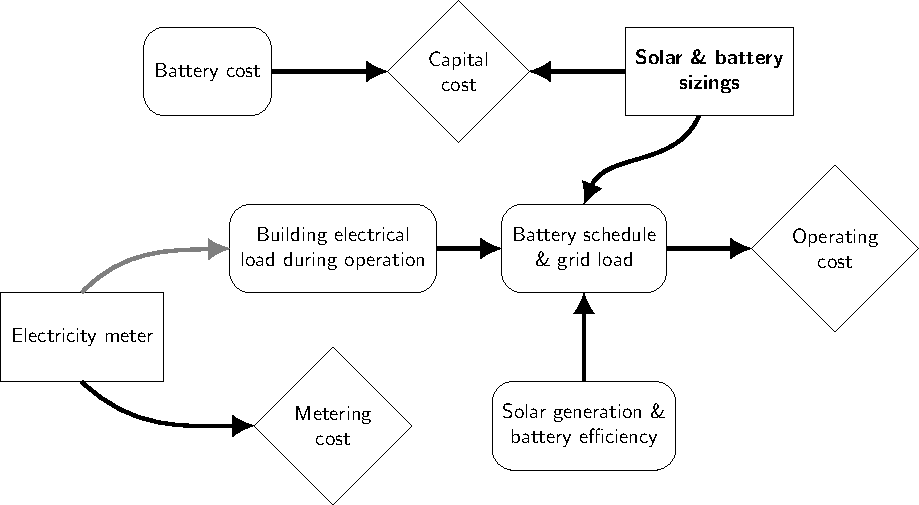
\includegraphics[width=0.75\linewidth]{Influence Diagram/building-design.pdf}
        \vspace*{0cm}
        \captionof{figure}{Influence diagram representation of example energy system design problem.}
        \label{fig:methodology-example-influence-diagram}
        \begin{singlespace}
            \raggedright
            \footnotesize{\it Square nodes represent decisions, rounded nodes represent uncertainties or uncertain factors, and diamond nodes represent outcomes or utilities/costs. Arrows represent causal dependencies between nodes, with grey arrows indicating reduction in uncertainty from data collection.}
        \end{singlespace}
    }
    \hfill\

    To understand how collecting the metering data and reducing load uncertainty might affect our design decision, we can look at the distribution of designs we would choose using our \glsxtrshort{sp} given the possible measurement values we might get. To do so, we hypothesise 50 possible true building load values, $\theta_{\text{load}}$, by drawing from the prior load distribution. We then hypothesise a possible measurement (previous annual load values we get from the metering data, $z_{\text{load}}$) for each true load value by drawing a sample from the corresponding likelihood function\footnote{This is the same as drawing from the joint prior distribution of $\theta$ and $z$.}. The information from each measurement is combined with the prior to form a posterior. And for each measurement value, we perform the design optimisation process by sampling load values from the corresponding posterior, and values for all other uncertainties from their priors as we assume we're not getting information about them, then using the \glsxtrshort{sp} to optimise over these `posterior scenarios' which have reduced load uncertainty.\\

    Fig. \ref{fig:methodology-example-post-designs} shows this distribution of `posterior designs'. Across the designs there is little change in the solar capacity, around $\pm$5\%, however the battery capacity chosen varies by $\pm$25\%. Before, we saw that accounting for uncertainty during the design process didn't have much affect on the chosen design. That is to say that the design that performs best \textit{on average} was similar to the best design for the average scenario\footnote{Specifically, we used the average annual load value in our deterministic optimisation. We're not sure how `average' the year of solar and load profile data we used is. Though there methods for coming up with an `average year' of data, and these are commonly used for energy system design.}.
    However we can clearly see that the uncertainty in building load \textit{does} have a significant effect on the best design for the actual building.\\

    {
        \centering
        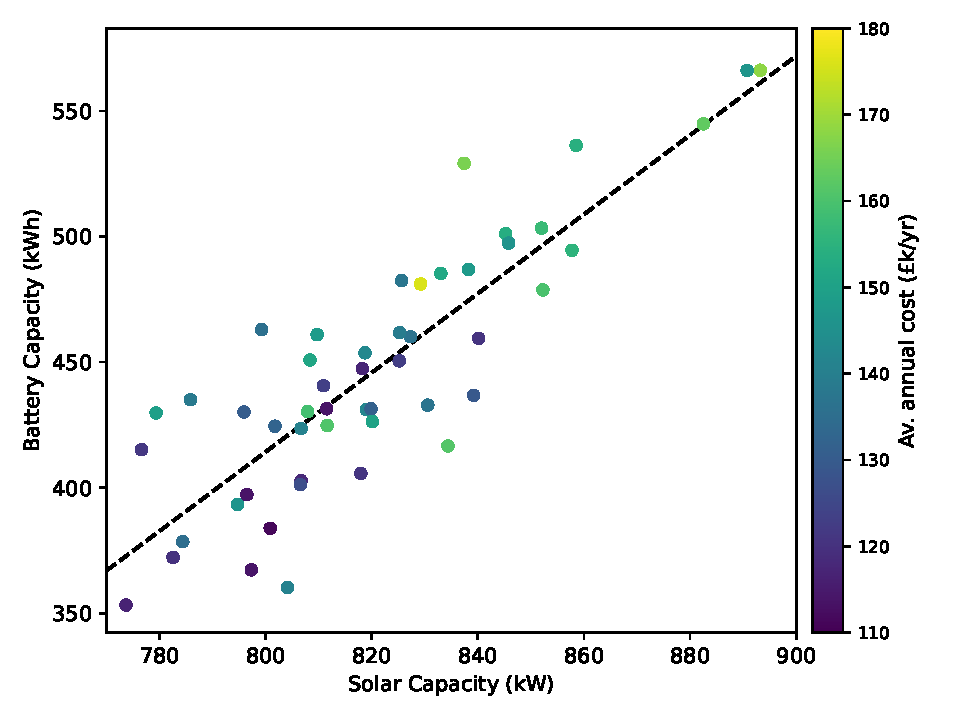
\includegraphics[width=0.75\linewidth]{Methodology/Figs/posterior_designs.pdf}
        \vspace*{-0.25cm}
        \captionof{figure}{Distribution of solar-battery system designs made with metering data.}
        \label{fig:methodology-example-post-designs}
    }
    \bigskip

\end{ebox}

\newpage
\section{The \glsxtrlong{voi}} \label{sec:methodology-voi}

The \glsxtrlong{voi} (\glsxtrshort{voi}) is defined as the difference in the performance of decisions made with and without extra information/uncertainty reduction. So, it is given by the difference between the expected utilities achieved by solving the Prior decision problem (Eq. \ref{eq:methodology-prior-optimisation}) and the Pre-Posterior decision problem (Eq. \ref{eq:methodology-preposterior-value}).
It numerically answers the question,
\begin{cbox}[colback=Aquamarine!10!white]{}
How much better could we do on average if we collected data to reduce the uncertainties in our problem before making a decision?
\end{cbox}
\vspace{0.2cm}

\noindent
If the decision problem has an economic objective (i.e. the utility is a cost or a profit), the \glsxtrshort{voi} tells us how much we should be willing to pay for the data that reduces the uncertainties in our problem. By comparing the \glsxtrshort{voi} to the cost of data collection, \textbf{we can determine if collecting that data is actually worthwhile for supporting our decision making}.\

\subsection{Perfect Information}

Initially let's consider the simplest case of \glsxtrshort{voi}, where we assume we have the ability to perfectly measure the system and remove all uncertainty from our problem. This means the data we collect tells us the true values of the uncertainties, $z=\theta$. So in this case the Pre-Posterior decision problem can be simplified, as the Posterior decision problem is now deterministic, we assume we know the true state of the system we want to optimise for,
\begin{equation}
    \mathlarger{
        \mathbb{E}_{\theta,z} \left\lbrace \max_{a \in \mathcal{A}} \: \mathbb{E}_{\vartheta|z}\lbrace u(a,\vartheta) \rbrace \right\rbrace
        \:\: \rightarrow \:\:
        \mathbb{E}_{\theta} \left\lbrace \max_{a \in \mathcal{A}} \: u(a,\theta) \right\rbrace
    }
\end{equation}
We find the \glsxtrshort{voi} by comparing the average utility achieved by these decisions made with perfect information to the average utility of the Prior decision problem, where the decision is made without any extra information about the uncertainties. In this case the \glsxtrshort{voi} is referred to as the \glsxtrlong{evpi} (\glsxtrshort{evpi}),
\begin{equation} \label{eq:evpi}
    \mathlarger{
        \text{EVPI} =
        \mathbb{E}_{\theta} \left\lbrace \max_{a \in \mathcal{A}} \: u(a,\theta) \right\rbrace
        - \max_{a \in \mathcal{A}} \: \mathbb{E}_{\theta} \left\lbrace u(a,\theta) \right\rbrace
    }
\end{equation}
The \glsxtrshort{evpi} provides an upper bound on all the other \glsxtrshort{voi} values. It is also much cheaper to compute as the posterior optimisations are deterministic. However \glsxtrshort{evpi} values can be misleading, as it's not practically possible to completely remove uncertainty, and so we cannot know how much of that value can actually be obtained.

\begin{ebox}[label=ebox:evpi]{Value of removing uncertainty}
    Let's imagine what would happen if we were able to perfectly know everything about our building and the solar-battery system we'll put into it, to see how much better we would do if we could achieve the theoretically best possible design. Of course this is unrealistic. Some of the uncertainties in the system couldn't be reduced, such as the pattern of solar generation during operation, and for the others, the uncertainty could never be completely removed. For example, we can't know the exact amount of energy the building will use during operation when we design it. But this thought experiment will give us some insight into how much these uncertainties are affecting our ability to make our design decision.\\

    To do this, we perform a similar process to \ref{ebox:bayes}, but we now sample scenarios from the prior distributions of all the uncertainties, and then use the \glsxtrshort{sp} to find the best design for each scenario, assuming that in each hypothesised case we knew the true values of the uncertainties.

    Fig. \ref{fig:methodology-example-perfect-information} compares the distribution of costs achieved by the initial/prior design (from Table \ref{tab:example-stoch-optimisation-results}) over the scenarios, to the costs of the best possible design for each scenario (the designs made with perfect information).\\

    {
        \centering
        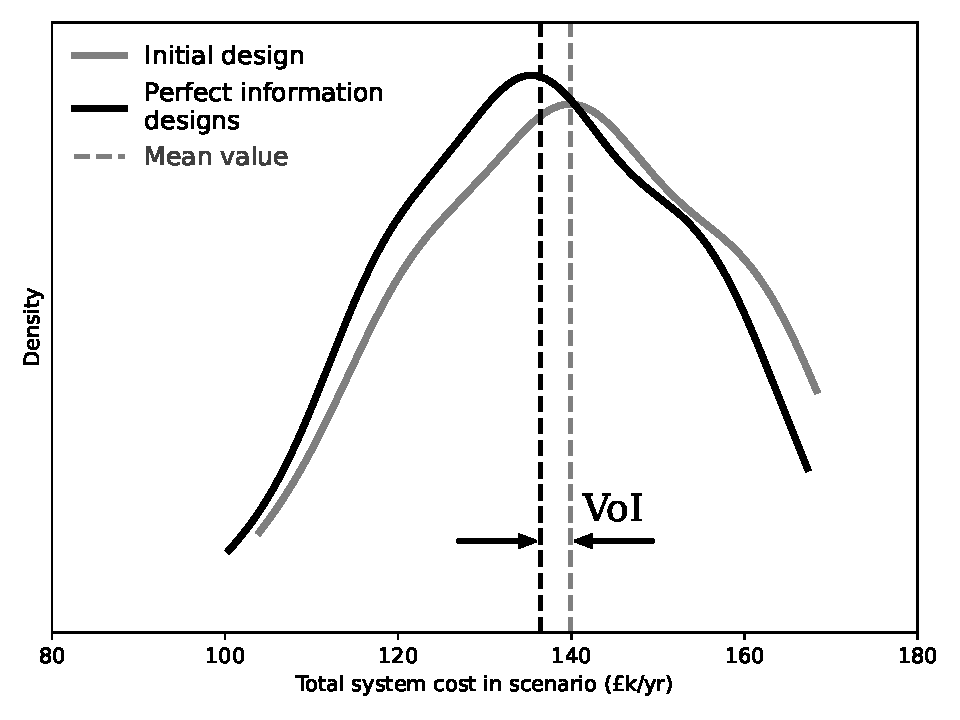
\includegraphics[width=0.75\linewidth]{perfect_info_costs_comparison.pdf}
        \vspace*{-0.25cm}
        \captionof{figure}{Comparing distributions of possible system costs for designs made with and without perfect information.}
        \label{fig:methodology-example-perfect-information}
    }
    \bigskip

    The average cost of the designs made with perfect information is £136.4k/yr. Comparing to the £139.9k/yr average cost of the initial design from \Cref{tab:example-stoch-optimisation-results}, the \glsxtrshort{evpi} is £3.5k/yr, or 2.5\% of the prior cost.

    In the context of improving energy system designs to reduce energy costs this is a pretty significant saving. However the \glsxtrshort{evpi} is only an upper bound. So we can't know how much of this cost saving we could actually achieve by collecting data in practice. All we can conclude from this is that reducing the uncertainties in our problem could save us \textit{up to} £3.5k/yr. So it \textit{might} be worth doing something about the uncertainties to improve our design decision. Or it might not.
\end{ebox}
\vspace{-0.25cm}

\subsection{Partial Perfect Information}

Often not all of the uncertainties in a system are, or even can be, reduced (see footnote \ref{fn:aleatoric}). So a more realistic case is one where some uncertainties are removed, but some others remain. This means in the Posterior decision problems, as not all uncertainties are removed, we need to optimise the average utility over the remaining uncertainties. Let's call the uncertainties that are removed by the data collection $\theta$, and the ones that remain unchanged $\phi$. In this case the \glsxtrshort{voi} is referred to as the \glsxtrlong{evppi} (\glsxtrshort{evppi}), and is given by,
\vspace*{-0.1cm}
\begin{equation} \label{eq:evppi}
    \mathlarger{
        \text{EVPPI} =
        \mathbb{E}_{\theta} \left\lbrace \max_{a \in \mathcal{A}} \mathbb{E}_{\phi} \: \lbrace u(a,\theta,\phi) \rbrace \right\rbrace
        - \max_{a \in \mathcal{A}} \: \mathbb{E}_{\theta,\phi} \left\lbrace u(a,\theta,\phi) \right\rbrace
    }
\end{equation}
\vspace{-0.6cm}

\begin{ebox}[label=ebox:evppi]{Designing with known load}
    Now, let's assume that we only removed the uncertainty in the annual energy usage of the building (or mean load), meaning that we knew perfectly at the time of design the aggregate energy demand we'd need to meet. In this case, the average cost of our designs made with perfect mean load information would be £139.4k/yr. So the \glsxtrshort{evppi} is just £0.5k/yr, or 0.4\% of the prior cost.

    This is a much smaller value than the \glsxtrshort{evpi} we calculated before, which tells us that the other uncertainties we're no longer removing\footnote{Which are in the cost and efficiency of the batteries, and the amount and pattern of solar generation.} have quite a big impact on our design decision. So removing this pretty significant uncertainty ($\pm$20\%) in the mean building load doesn't provide us that much of a cost saving for our design. We may decide that it's not worth chasing this saving, and so the upper bound we get from this simplified case can tells us that this information isn't worthwhile collecting.
\end{ebox}


\subsection{Imperfect Information}

In the general case, collecting data reduces but does not remove uncertainties\footnote{The previous perfect info. cases are just special cases of this, and provide an upper bound on this general value, \vspace*{-0.3cm}\begin{equation*} \mathbb{E}_{\theta,z} \big\lbrace \max_{a \in \mathcal{A}} \: \mathbb{E}_{\vartheta|z}\lbrace u(a,\vartheta) \rbrace \big\rbrace \leq \mathbb{E}_{\theta} \big\lbrace \max_{a \in \mathcal{A}} \: u(a,\theta) \big\rbrace \end{equation*}\vspace*{-0.55cm}}.
We refer to this as gathering `imperfect information'. How we model uncertainty reduction from data and understand its effect on decision making is discussed in \Cref{sec:methodology-bayesian-decision-analysis}. If we have some measurement option $e$ available, which has likelihood function $f_e(z|\theta)$, the value of the information provided by that measurement is referred to as the \glsxtrlong{evii}\footnote{The \glsxtrshort{evii} is also commonly referred to as the \glsxtrlong{evsi} (\glsxtrshort{evsi}) \citep{keisler2014ValueInformationAnalysis}.} (\glsxtrshort{evii}), and is given by,
\begin{equation} \label{eq:evii}
    \mathlarger{
        \text{EVII}(e) =
        \mathbb{E}_{\theta,z} \left\lbrace \max_{a \in \mathcal{A}} \: \mathbb{E}_{\vartheta|z}\lbrace u(a,\vartheta) \rbrace \right\rbrace
        - \max_{a \in \mathcal{A}} \: \mathbb{E}_{\theta} \left\lbrace u(a,\theta) \right\rbrace
    }
\end{equation}
which is just the difference between the prior decision utility (Eq. \ref{eq:methodology-prior-optimisation}) and the pre-posterior decision utility (Eq. \ref{eq:methodology-preposterior-value}).\\

The greater the uncertainty reduction provided by the measurement, the larger the \glsxtrshort{evii}. So when there are multiple measurement options available, we can compare the improvements in decision making performance they provide to their costs, and determine which measurement (if any) is most economical for supporting our decision making. Fig. \ref{fig:methodology-EVII-precision-cost-curve} illustrates this trade-off between the usefulness and cost of more precise measurement.

\vspace*{-2ex}
\pgfplotsset{
  layers/axis lines on top/.define layer set={
    axis background,
    axis grid,
    axis ticks,
    axis tick labels,
    pre main,
    main,
    axis lines,
    axis descriptions,
    axis foreground,
  }{/pgfplots/layers/standard},
} % from https://tex.stackexchange.com/questions/240359/tikz-axis-border-on-top-grids-below

\begin{figure}[h]
    \centering
    \vspace*{0.25cm}
    \resizebox{0.8\textwidth}{!}{
    \begin{tikzpicture}
        \def\N{100}
        \def\C{5}
        \def\xmax{10}
        \def\ymin{-0.1}
        \def\ymax{1.2}
        \def\xopt{2.44102} % from desmos
        \def\yopt{0.92817} % from desmos
        \def\xint{5.46579}

        \begin{axis}[
            set layers=axis lines on top,
            every axis plot post/.append style={
                mark=none,domain={0}:{10},samples=\N,smooth},
                xmin={-1}, xmax=\xmax,
                ymin=\ymin, ymax={\ymax},
                axis lines=middle,
                axis line style=thick,
                enlargelimits=upper, % extend the axes a bit to the right and top
                %ticks=none,
                xlabel={\large $\sigma^2$},
                ylabel={\glsxtrshort{evii}},
                xtick={{10}},
                xticklabels={{$\sigma^2_{\text{prior}}$}},
                ytick={{1},{0.75}},
                yticklabels={{\normalfont \glsxtrshort{evpi}},{\large $c(e)$}},
                every major tick/.append style={thick, major tick length=7pt, black!50},
                every axis x label/.style={at={(current axis.right of origin)},anchor=west},
                every axis y label/.style={at={(current axis.above origin)},anchor=south},
                width=0.7*\textwidth, height=0.4*\textwidth,
                y=4cm,
                clip=false,
                %every tick label/.append style={font=\scriptsize}
            ]

        \draw[draw=none, left color=red!30, right color=red!10!white] (axis cs:\xint,0) rectangle (axis cs:\xmax,\ymax);

        \addplot[black!25,ultra thick,name path=D] {0.75-x/15};
        \addplot[black,ultra thick,name path=B] {1-sig(x,\C)};
        \addplot[black,ultra thick,dashed,name path=C] {1};

        \draw[ultra thick, green!50!black!50, arrows = {Stealth[inset=0pt, angle=60:6pt]-Stealth[inset=0pt, angle=60:6pt]}, shorten >= .5mm, shorten <= .5mm] (axis cs:\xopt,0.75-\xopt/15) -- (axis cs:\xopt,\yopt);
        %\draw[ultra thick, red!50] (axis cs:\xint,0) -- (axis cs:\xint,\ymax);

        \node[draw=none] at (axis cs:\xopt-0.8,0.475) {\scriptsize Best measurement};
        \node[draw=none] at (axis cs:7.75,0.75) {\footnotesize Not economical};

        \end{axis}
    \end{tikzpicture}
    }
    \vspace*{-0.25cm}
    \caption{Illustrative EVII vs. measurement cost curve} \label{fig:methodology-EVII-precision-cost-curve}
\end{figure}

However we don't just need to compare different levels of reduction of the same uncertainty. As long as we can come up with a probabilistic model for the measurements, we can compare the benefit of reducing different uncertainties or combinations of them. When we're thinking about reducing multiple uncertainties in our problem we have to be careful, as the combination of uncertainty reductions can have a significant effect on the \glsxtrshort{voi}. This is referred to as `system effects' \citep{difrancesco2023SystemEffectsIdentifying}. \glsxtrshort{voi} values don't add.
If two measurements provide complementary information then the \glsxtrshort{voi} of the combination can be substantially greater. For example, when `smart charging' an electric vehicle in a car park, knowing the state-of-charge of the vehicle may only be useful if we also know how long it'll be parked for, as only then can we know whether there's enough time to adjust the charging schedule.
On the other hand, two measurements can contain redundant information, meaning the second provides little extra value. For example, supply/return water temperatures and heat meters provide similar information about a building's heating load.\\

\begin{ebox}[label=ebox:evii]{Designing with energy usage data}
    Returning to the building electricity meter data we used in \ref{ebox:bayes} to reduce uncertainty in the annual energy usage, let's now look at the value of that information for supporting our design decision. Fig. \ref{fig:methodology-example-post-designs-comparison} compares the designs we would make with reduced load uncertainty to the initial design we would make with only the prior information, as well as the average cost of each design over the remaining uncertainty.

    {
        \centering
        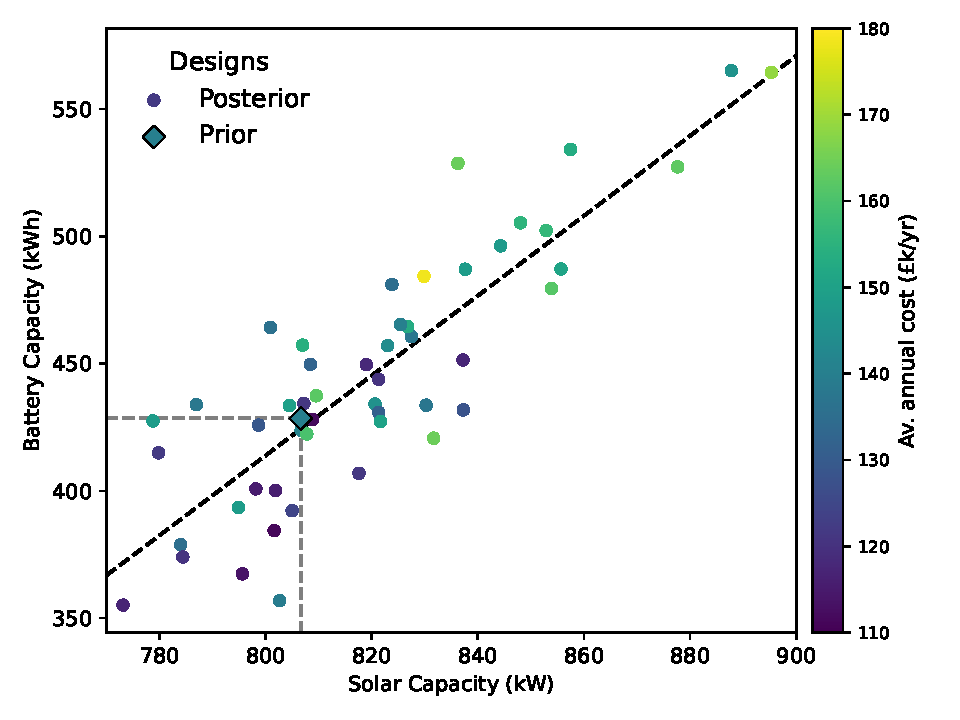
\includegraphics[width=0.75\linewidth]{prior_vs_posterior_designs.pdf}
        \vspace*{-0.25cm}
        \captionof{figure}{Comparison of initial design and designs made with reduced load uncertainty.}
        \label{fig:methodology-example-post-designs-comparison}
    }
    \bigskip

    As we commented last time, getting this information and reducing the load uncertainty leads us to significantly change our design choice, and we can end up making a design decision quite different from the initial choice we'd make (the prior design). Also, the expected cost of the system varies substantially ($\pm$25\%) over the possible load measurements we could receive. This seems to suggest that the load uncertainty is having a significant impact on our decision making, as reducing it leads to large changes in both decision and cost.\\

    But ultimately we're not actually interested in the choice we end up making. Instead, what we care about is how good a job we can do at solving our problem. The average cost of the designs made with reduced load uncertainty is £139.7k/yr. Meaning the \glsxtrshort{evii} is just £0.2k/yr, or 0.2\% of the prior cost. This is around half the \glsxtrshort{evppi} value from \ref{ebox:evppi} (\Cref{tab:example-voi-summary} below gives the comparison). This means that, even though the practical measurement removes around 75\% of the uncertainty, it's only providing us with 50\% of the benefit for decision making.

    From this perspective, reducing load uncertainty in fact isn't particularly important to our decision making. It wouldn't be worth spending much money collecting this data, as the improvement it provides to our design decision is very small.

    However, it does significantly reduce our uncertainty in how much our energy system will cost, which may be beneficial for financial planning and risk management. This is explored in more detail in \Cref{chap:districts}.\\

    {\centering
    \renewcommand{\arraystretch}{1.25}
    \begin{tabularx}{0.8\linewidth}{cccr@{\hskip .75ex}l}
        \toprule \toprule
        \makecell{Case} & \makecell{From} & \makecell{Av. total cost of\\[-.5ex]design(s) (£k/yr)} & \multicolumn{2}{>{\centering\arraybackslash}c}{\makecell{VoI (£k/yr)}} \\
        \midrule \midrule
        %\multicolumn{5}{>{\centering\arraybackslash}l}{\small\it Discrete design options} \\
        \makecell{No uncertainty\\[-.5ex]reduction (prior)} & \makecell{\Cref{tab:example-stoch-optimisation-results}\\[-.5ex]{\small(\glsxtrshort{sp} soln.)}} & 139.9 & \multicolumn{2}{>{\centering\arraybackslash}c}{--} \\
        Imperfect information & \ref{ebox:evii} & 139.7 & 0.2 & (\glsxtrshort{evii}) \\
        \makecell{Partial perfect\\[-.5ex]information} & \ref{ebox:evppi} & 139.4 & 0.5 & (\glsxtrshort{evppi}) \\
        Perfect information & \ref{ebox:evpi} & 136.4 & 3.5 & (\glsxtrshort{evpi}) \\
        \bottomrule \bottomrule
    \end{tabularx}
    \bigskip
    \vspace*{-0.5ex}
    \begin{singlespace}
    \parbox[]{0.8\linewidth}{
    \captionof{table}{Summary of designs made with different levels of uncertainty reduction and associated \glsxtrshort{voi} values.} \label{tab:example-voi-summary}
    }

    \vspace*{-0.5ex}
    \raggedright
    \footnotesize{\it Remember that for the partial and imperfect information cases, only uncertainty in the building load was being reduced. We could potentially get somewhat closer to the \glsxtrshort{evpi} value by also reducing the uncertainty in the battery cost and efficiency, for example, by negotiating with a manufacturer and doing our own tests on the batteries. But we could never reduce our uncertainty in the amount and pattern of solar generation.}
    \end{singlespace}
    }

\end{ebox}


\subsection{Information theoretic \glsxtrshort{voi}}

There is also an information theoretic view on \glsxtrshort{voi}. It takes a purely statistical perspective, and defines the utility as the information content or statistical `surprise' of the outcomes\footnote{`Surprise' is a statistical measure of how surprising or unlikely an outcome is. The more unlikely an outcome, the more you learn (the more information you get relative to the prior) by observing it.}. This means that the expected utilities become entropies,
\begin{equation}
    \mathlarger{u(\theta) = -\log p(\theta) \implies \mathbb{E}_{\theta} \lbrace u(\theta) \rbrace = \sum_{\theta} \left( - p(\theta) \log p(\theta) \right) = H(\theta)}
\end{equation}

\noindent
And so the \glsxtrshort{voi} is the mutual information between the uncertainties and the measured data,
\begin{equation}
    \mathlarger{\text{VoI}(e) = \mathbb{E}_{\theta} \lbrace u(\theta) \rbrace - \mathbb{E}_{\theta,z} \big\lbrace \mathbb{E}_{\vartheta} \lbrace u(\vartheta|z) \rbrace \big\rbrace = H(\theta) - H(\theta|z) = I(\theta\,;z)}
\end{equation}
\smallskip

\noindent
As this view of \glsxtrshort{voi} is purely statistical, it doesn't require a decision making model. This is both an advantage and a flaw. It means that we can calculate \glsxtrshort{voi} values for measurements/uncertainty reduction without having to develop a potentially complicated model of how that uncertainty will be used to information decision making. But as a result, we lose a lot of the interpretability of \glsxtrshort{voi}. The units of \glsxtrshort{voi} are now information `bits', and we cannot know how useful that information will be for supporting our decision making, which is ultimately what we care about. This approach is most useful for comparing the uncertainty reduction provided by different measurements in complex systems\footnote{If the system is too simple the likelihood functions of the measurements already tell us what we need to know.}, and looking at the trade-off between the number of measurements made and total uncertainty reduction.\\

\vspace*{0.5cm}

\section{Framework extensions} \label{sec:methodology-framework-extensions}

The decisions that need to be made in real-world engineering problems have complexities that cannot be handled by the standard \glsxtrshort{voi} framework that we've seen so far. This section presents two extensions to the framework that allow us to investigate the value of uncertainty reduction to improve decision making in more complex settings.

Firstly, `On-Policy' \glsxtrshort{voi}, which is a novel framework extension and contribution of this thesis, that allows the \glsxtrshort{voi} to be studied in complex systems where direct optimisation is not possible. And secondly, the \glsxtrlong{voo} (\glsxtrshort{voo}) framework, which allows the benefit of retaining decision optionality as uncertainty reduces to be studied.

\subsection{On-Policy \glsxtrlong{voi}} \label{sec:methodology-on-policy-voi}

So far, the \glsxtrshort{voi} calculations have assumed that we have access to an accurate model of the system that we are able to optimise to find the decision/action that provides the highest expected utility, and also tell us that expected utility. However, many practical engineering problems are too complex for an accurate model of the system to be optimised directly. Instead, decisions are made using policies, such as Rule-based Control, Reinforcement Learning, or \glsxtrlong{sp}. These policies either use heuristics to guide their choice of, or search through, actions, or they simplify the system model and/or the statistical representation of the uncertainties\footnote{The most common example of this is the use of Monte Carlo approximations of the expected utility which use only a small number of samples to limit the computational cost of the model, but come at the expense of significant statistical error in the estimate.} and/or the optimisation objective (utility model), to provide an approximate model that is computationally manageable and can be optimised. As a result, a policy may not provide a sufficiently accurate\footnote{Or in some cases even estimate the expected utility at all.} estimate of the expected utility to provide useful \glsxtrshort{voi} values. I.e. the errors in the expected utility estimates may be larger than the \glsxtrshort{voi}, and lead to extremely noisy \glsxtrshort{voi} estimates.\\

To extend the standard \glsxtrshort{voi} framework to allow decision making via policies, an additional step is added to the computations, which estimates the expected utility achieved by the actions selected by the policy using a more accurate model of the system, uncertainties, and utility.

A decision policy is defined as a mapping from a utility function describing a system, $u(a,\theta)$, and a distribution describing the uncertainties in the system, $\pi(\theta)$, to an action,
\begin{equation} \label{eq:policy-defn}
    \mathlarger{\mathcal{P} \left( u(a,\theta),\pi(\theta) \right) \rightarrow \alpha \in \mathcal{A}}
\end{equation}

As the utility function and set of possible actions are constant when we're looking at a given decision problem, we'll simplify the notation and refer to a policy applied to a given decision problem as $\mathcal{P}_u(\pi(\theta))$. The action selected by the policy therefore depends on the uncertainties in the system\footnote{However we don't impose any conditions on how the policy uses the statistical information about the uncertainties, $\pi(\theta)$. The policy could be deterministic. For example, it could use only the expected (or maximum likelihood) values of the uncertainties from the distribution. In fact, this is what the \glsxtrlong{evp} does, and so it is a heuristic policy.\\[-1.5em]

\noindent \textit{When policies don't make use of information about uncertainty, understanding how uncertainty reduction affects their ability to make decisions is, if anything, more important. The \glsxtrshort{evp}, for example, cannot hedge its decisions, and so may be more reliant on good data.}}.\\

The \glsxtrshort{voi} calculations proceed in the same way as before (compare to Eq. \ref{eq:evii}), but instead of selecting actions using a stochastic optimisation, they are now selected by applying the policy to the relevant distribution of uncertainties, and the expected utility those actions achieve needs to be evaluated using the utility function/model.
\begin{equation} \label{eq:OP-voi}
    \mathlarger{
        \text{EVII}_{\mathcal{P}}(e) =
        \mathbb{E}_{\theta,z} \left\lbrace \mathbb{E}_{\vartheta|z} \left\lbrace u\!\left( \mathcal{P}_u\!\left(\pi (\theta|z)\right)\!,\vartheta \right) \right\rbrace\!\!\right\rbrace
        - \mathbb{E}_{\theta} \left\lbrace u\!\left(\mathcal{P}_u\!\left(\pi (\theta)\right)\!,\theta \right)\!\right\rbrace
    }
\end{equation}
where the $\mathcal{P}$ subscript indicates that this is the value of uncertainty reduction for supporting decisions made using policy $\mathcal{P}$.\\

This framework extension is called `On-Policy \glsxtrlong{voi}', as the decisions are made using a specific policy, and so the benefit of data collection/uncertainty reduction calculated is now dependent on the policy used. This broadens one of the main criticisms of the \glsxtrshort{voi} framework, namely that \glsxtrshort{voi} values do not generalise. This criticism is discussed further in \Cref{sec:methodology-limitations}. However, this does also open up the opportunity to study how different policies benefit from uncertainty reduction, and which are best able to exploit improved statistical information.

The key advantage of On-Policy \glsxtrshort{voi} is that is allows us to study the value of information for complex, practical engineering problems where decision policies have to be used. For instance, problems with high-dimensional actions (i.e. where a large number of decisions must be made simultaneously), or those with tight computational limitations.\\

\begin{ebox}{Using a decision policy}
    Throughout our example problem we've been using a Stochastic Program, specifically a linear scenario program, to perform our design optimisation and make decisions for us. This \glsxtrshort{sp} uses a simplified model of the energy system, it is linearised and assumes perfect foresight. Also, to keep the computation time manageable, when we solve the posterior decision problems we've only been using 10 samples from the posterior distributions of the uncertainties, leading to quite a noisy estimate of the expected utility.

    So we are actually already using a policy to make our decisions. And there's potentially quite a bit of error in our estimate of the expected utility from both the model and statistical simplification. We could create a more accurate simulator of our building energy system, and apply it to more samples from the posterior distributions to get a more accurate estimate of the expected utilities, and use this to do an On-Policy \glsxtrshort{voi} calculation. However this is a bit too complicated for our simple example.
    You can see On-Policy \glsxtrshort{voi} calculations for a more complex building energy system in \Cref{chap:districts}.
\end{ebox}


\subsection{\glsxtrlong{voo}} \label{sec:methodology-optionality}

% OG paper with similar idea \citep{merkhofer1977ValueInformationGiven}. \citep{zhang2021ValueInformationAnalysis} also includes this as a framework extension (they call it EVSIA), so it's not new

Standard \glsxtrshort{voi} calculations also assume that when decisions are made with and without data collection/uncertainty reduction, the set of possible actions is the same. However in many practical engineering problems, collecting data leads to a delay\footnote{This delay may form part of the cost of collecting data.} before the decision is taken, and keeping decision options available through this delay is costly, even if those options do not end up being used.\\

We can adapt the \glsxtrshort{voi} framework to study the effect that changing the set of available actions has on decision making as uncertainty is reduced. This is referred to as the \glsxtrlong{voo} (\glsxtrshort{voo}).

If after data collection, the set of available actions is reduced from an initial set, $\mathcal{A}$, to a smaller set, $\mathcal{B} \subset \mathcal{A}$. Then the improvement in decision making that would be achieved by maintaining optionality, and keeping the original set of actions for the decision made with reduced uncertainty, referred to as the \glsxtrlong{evo} (\glsxtrshort{evo}), is given by,

\begin{align}
\begin{split} \label{eq:methodology-voo}
    \mathlarger{\text{EVO}(\mathcal{B},e)} \:
    &\mathlarger{
        = \mathbb{E}_{\theta,z} \left\lbrace \max_{a \in \mathcal{A}} \: \mathbb{E}_{\vartheta|z}\lbrace u(a,\vartheta) \rbrace \!\right\rbrace - \mathbb{E}_{\theta,z} \left\lbrace \max_{a \in \mathcal{B}} \: \mathbb{E}_{\vartheta|z}\lbrace u(a,\vartheta) \rbrace \!\right\rbrace
    }\\[1ex]
    &\mathlarger{
        = \mathbb{E}_{\theta,z} \left\lbrace \max_{a \in \mathcal{A}} \: \mathbb{E}_{\vartheta|z}\lbrace u(a,\vartheta) \rbrace - \max_{a \in \mathcal{B}} \: \mathbb{E}_{\vartheta|z}\lbrace u(a,\vartheta) \rbrace \!\right\rbrace
    }
\end{split}
\end{align}
Notice that the inner term is zero unless we use the optionality and choose an action outside of the reduced set $\mathcal{B}$ when data $z$ is collected. This equation could also be expressed as a difference of \glsxtrshort{voi} values.\\

Similarly to the \glsxtrshort{voi}, the \glsxtrshort{voo} tells us how much better we do on average at solving our problem by maintaining optionality and being able to choose from the full set of actions\footnote{We could also investigate the benefit of increasing the set of actions available to us.} when uncertainty has been reduced. By comparing the benefit optionality provides to decision making to the cost of keeping those options available, we can determine if maintaining optionality is worthwhile.\\

\begin{ebox}{Exploring optionality}
    For the design of our building energy system, we likely have a number of different options for decarbonising the energy usage. For example, instead of installing Li-ion battery storage we could instead install heat pumps, a hot water storage system, or mechanical ventilation with heat recovery (MVHR). We will likely go through an initial design phase and choose one of these approaches. After this, we'll do a more detailed design of the system, and gather some data about the building to help with this, for instance the historic electrical \& heating loads and more precise data on the specs of our chosen system. However, the best decarbonisation approach depends on how much electricity and heat the building will use, and how our energy system performs. So after we've reduce these uncertainties we may find out a different approach than the one we initially chose would actually be better. But we're committed now.

    We could perform a \glsxtrshort{voo} calculation to see how much we could save by doing a preliminary design for all configurations of the energy system, gathering the building load data and tech specs from the equipment manufacturers, and then choosing the best approach after the uncertainties have been reduced. With this we could determine whether the extra time and effort required to provide this optionality is worthwhile, or if our initial design choice is good enough.

    Again, doing this calculation is a bit complicated for our simple example. But a \glsxtrshort{voo} calculation is performed in the context of energy storage technology selection for an industrial scale energy park in \Cref{chap:parks}.
\end{ebox}\


%********************************** VoI discussions **************************************
\section{Limitations of framework} \label{sec:methodology-limitations}

% lack of generalisation guarantees (though this applied to lots of engineering analyses, VoI can be particularly sensitive, discuss why?) - overcome with sensitivity analysis (but even more expensive)
% models are necessarily limited, so some judgement is needed at to whether it's good enough; particularly difficult as adding in new uncertainties (even non-reducible) can change the VoI, so model completeness is a concern
% computational cost, we need to do optimisation based design potentially hundreds of times - limits model complexity, accuracy, and scope
% it also requires to actually be able to come up with a decision model of the system - can only be used for automated decision making with a single objective (no multi-objective), this modelling is hard, and we can't account for more holistic factors in decision making
% only VoI contained within model is accounted for, there may be other uses for the data collected that aren't captured in the decision model, e.g. unknown future uses, or retro-active decisions - though in this case it gives us a much more defined value to guess (gap between VoI and collection cost)
% assumption of risk neutrality - overcome with risk aversion utility functions (e.g. CVaR in Chap:districts)

The key limitation of \glsxtrshort{voi} analysis is that the \glsxtrshort{voi} values calculated are only valid for the particular system model, statistical model, decision objective, and policy used. The framework does not provide any guarantees that the conclusions about which and how much data should be collected will generalise to other systems, or even with changes to the current model and its assumptions. So care needs to be taken when interpreting and communicating the insights provided by the \glsxtrshort{voi}, being clear that the conclusions only apply to how data collection is used to support the specific decision made within the assumptions and limitations of the model. Of course this is a very common limitation of engineering analyses, particularly optimisation modelling. Generalisation guarantees are difficult to provide, and at some point judgement is required as to whether a model is a good enough representation of the practical engineering problem. However, \glsxtrshort{voi} can be particularly sensitive to the model setup. This is because \glsxtrshort{voi} values depend on the utility values at the optima, which can move significantly and unexpectedly as the model changes. Seemingly innocuous changes to the model can cause large changes in \glsxtrshort{voi}, for example if they lead to a dominant action which causes the \glsxtrshort{voi} to drop to zero. Adding new uncertainties into the model can also affect the \glsxtrshort{voi}, even if those uncertainties are not measured and reduced.

This generalisation limitation can be overcome by performing sensitivity analyses to test whether the conclusions drawn remain valid as the model setup and assumptions change. However, this is very computationally expensive, and it's not possible to test all model variations that could be relevant. Particularly as performing \glsxtrshort{voi} calculations is already highly computationally expensive.\\

The second main limitation is the computational cost of calculating the \glsxtrshort{voi}. In \glsxtrshort{voi} analysis we are testing how the decision optimisation changes as different data values are observed. Outside of very simple analytic cases, this requires us to sample possible data values and repeat the decision optimisation a large number of times to get a good \glsxtrshort{mc} estimate of how well we can do on average when making decisions with data. So computing a single \glsxtrshort{voi} value requires likely hundreds of optimisations to be performed. For practically useful problems, these optimisations are themselves computationally expensive. This means that either expensive compute resources\footnote{The optimisations needed for \glsxtrshort{voi} calculations are embarrassingly parallel. So calculations can be performed quickly if enough compute is available.} are needed, the scope of problems considered needs to be limited, or significant simplifications need to be made to the model, which can affect the accuracy of the results. For the \glsxtrshort{voi} calculations in Chapters \ref{chap:districts} \& \ref{chap:parks}, a supercomputer\footnote{The experiments were run using the Cambridge Service for Data Driven Discovery (CSD3, \url{www.csd3.cam.ac.uk}).} was needed to run the experiments in an achievable time.

To be able to perform the decision optimisations, we also need to be able to develop a decision-making model of the engineering system, be that a system model that can be optimised or a suitable decision policy. For complex, real-world engineering systems this modelling can be extremely challenging and require significant domain expertise. The \glsxtrshort{voi} framework also requires that we describe outcomes with a single utility value. This means it is not compatible with multi-objective decision making and cannot account for subjective factors of decision making that often occur in engineering design. The framework is most suited to automated or model-based decision making.\\

\glsxtrshort{voi} calculations investigate the impact that data has on the decision model being tested. So, when interpreting the \glsxtrshort{voi} values that we receive from the analysis and making judgements about whether data should be collected, we are assuming that the decision model provides a sufficiently good representation of the physical engineering system we care about. Specifically, we assume that the usefulness of data in the model is the same as in the real system. While the \glsxtrshort{voi} framework studies the quality of data in detail, it does not have any mechanism for accounting for the quality of the model. The On-Policy \glsxtrshort{voi} methodology presented in \Cref{sec:methodology-on-policy-voi} provides some route to addressing this limitation, as the decision model (policy) and evaluation model (utility) are separated, allowing a more computationally expensive, and hopefully more accurate model to be used to evaluate the effect of the decisions on the system. But it still requires the assumption that this more accurate model is a good enough representation of the real system.

This limitation of model quality is inherent to analyses concerned with design, as the system does not yet exist, and so cannot be measured to validate the model. Expert judgement and experience of other systems is needed to assess whether a particular model is good enough to provide trustworthy \glsxtrshort{voi} values. However, in some cases we can justify that the model used for \glsxtrshort{voi} is, in a certain sense, exact. This is because \glsxtrshort{voi} is concerned with how uncertainty affects decision making. If we have access to the decision model that real-world practitioners use to make their decisions, then using that model in the calculations tells us exactly how uncertainty affects those decisions. For example, many energy systems are designed using linear stochastic program models. The analysis in \Cref{chap:districts} tells us exactly how a designer using such a model is affected by building load uncertainty, and how useful load data is to them. So in an industry setting, \glsxtrshort{voi} analyses can use the actual decision making models. This is, provided they are computationally feasible. Using a simplified model would lead to the same quality limitations.

The model quality includes not only the accuracy of the physics of the system, but also the statistical models of the uncertainties and data. \glsxtrshort{voi} calculations can be sensitive to these statistical models, but must assume that they are correct\footnote{However, precisely defining what it is for a predictive statistical model to be inaccurate, and identifying how this inaccuracy affects the \glsxtrshort{voi}, is not an easy task. After all, a prior distribution represents our best knowledge about an unknown quantity. Considering whether this knowledge is wrong can lead to pathological and unhelpful analyses.}. This includes aspects such as the resolution of the data in the model, and correlations between uncertain variables.\\

We collect data for many reasons, and data has many uses. However, \glsxtrshort{voi} calculations only quantify the value of data collection to support the specific decision studied. So if that same data is useful for other purposes not captured by the model, this extra value will be missed by the calculated \glsxtrshort{voi}. It's difficult, for example, to describe how useful having a historic record of some measurement of a system might be to inform future decision making, such as maintenance. However, having the \glsxtrshort{voi} value helps us make these finer judgements about whether data is worthwhile collecting. With knowledge of the value of that data for supporting the known and modellable decisions, and the cost of collecting the data, we only need to judge whether we think the extra value we might get from the data justifies that difference between the known benefit and the cost. And it may turn out that the data is already worth collecting on the basis of the known decisions.\\

Finally, the standard \glsxtrshort{voi} framework assumes that decisions are made in a risk-neutral way. This comes from the optimisation objective being the expected/average utility. However many real-world decision makers are risk averse, particularly those making large financial investments to decarbonise energy. The framework can easily be adapted to account for risk aversion in decision making by including it the decision objective. This allows us to study how uncertainty reduction affects decision risk, as is done in \Cref{chap:parks}.\\

\begin{ebox}{Understanding and overcoming our limitations}
    % What are the limitations in our example? And what could we do to overcome them?
    In our example problem, we found that collecting electricity meter data to reduce the uncertainty in the building load provided little benefit for improving our design decision of sizing the solar-battery system. But the calculations we've done only apply to the specific building energy model we've used, the probabilistic models of the uncertainties, and our decision objective. All of these contain simplifications and assumptions which might not be the same for other buildings. So to make a more general statement about the value of energy usage data for supporting building energy system design, we'd need to see whether our conclusion stays the same when we adapt our model to the properties of other buildings. For example, domestic buildings will have different load distributions and energy sale prices.

    To make our example computationally achievable, we've had to make some significant simplifications to the building energy model. We've linearised the physics and assumed perfect foresight. Potentially if we used a more realistic model we might get quite different cost values, which could alter the \glsxtrshort{voi}. There are also some uncertainties we haven't included in the model, for example uncertainty in the cost of solar panels, which might also affect the \glsxtrshort{voi}.

    To keep the computation time down, we had to use quite a small number of samples from the posterior distributions. So there might be quite significant statistical error in our estimate of the \glsxtrshort{voi} values. To test this, we should perform some more samples and see whether the \glsxtrshort{voi} values change significantly, or whether the estimates have already converged.
\end{ebox}\


% \section{Computing \glsxtrshort{voi} in practice} \label{sec:methodology-considerations}

% \subsection{Modelling the problem}

% The hardest part of VoI is modelling the problem. Here are the components you need ...

% \subsection{Computational workflow}

% Nice flow diagram of generalised workflow explaining each step - adapt workflow from BD-VOI methodology section - link to influence diagram

% \subsection{Improving computational efficiency}

% The main bottleneck in VoI calculations is the computational cost (getting it low enough to actually get a decent statistical estimate of the VoI), so here are some considerations to improve the efficiency of the calculations

% Probably keep each subsection brief and just mention the possible options to explore

% \subsubsection{Modelling choices} \label{sec:methodology-modelling-choices}

% Both for probabilistic models and for decision models

% Discretisation, linearisation/convexification, analytic approximations \citep{wilson2015PracticalGuideValue} (much stricter modelling assumptions), surrogate models (e.g. GPs - sort of numerical/analytic hybrid), etc. - trade-off of speed and accuracy

% \subsubsection{Accelerating computation}

% Fundamental parallelisability, ability to split up statistical and optimisation parts, etc.

% \subsubsection{Statistical techniques}

% Importance sampling?, scenario reduction methods, etc.; trying to get more accurate estimates with fewer samples

% \subsubsection{Understanding accuracy}

% Discuss open problem of VoI accuracy estimation


\newpage
%********************************** Model definition appendix  **************************************
\begin{subappendices}

\section{Simple building energy system model for example problem} \label{app:example-problem-formulation}

% Intro and explain simple energy system model, why we use a Linear Program, how it works in simulation and design mode, etc.

For our example problem of designing (specifically sizing) a solar-battery system for a commercial building, we'll consider a simplified model of the building energy system. This system has four key components: the building electrical load which needs to be met (we'll assume the heating is electrified), the solar panels which generate electricity, the battery storage system which can store and release electricity, and the grid from which we can buy and sell electricity. Fig. \ref{fig:example-system-diagram} illustrates the energy flows in this energy system model.

\begin{figure}[h]
    \centering
    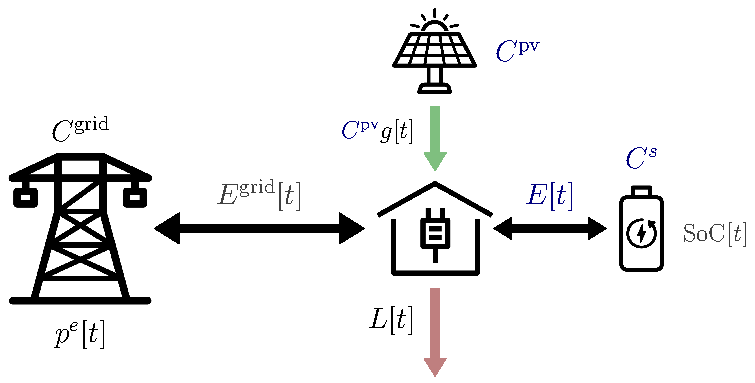
\includegraphics[width=0.75\linewidth]{System Diagram/sys-diagram.pdf}
    \caption{Illustration of energy flows in example building energy system.} \label{fig:example-system-diagram}
\end{figure}

\subsection{Energy model}

We can create a linear model of the behaviour of this energy system by assuming that the only physics we need to satisfy is the conservation of energy, and that the properties of the solar panels and battery storage system (e.g. efficiency, power limits, etc.) are fixed/constant. We will treat the building load, generation potential of the solar panels, and price of grid electricity as exogenous, but potentially uncertain.

Our goal is to design the system to minimise the total cost of meeting the building's energy demands. This is made up of the cost of installing the solar panels and battery storage, the cost of buying electricity from the grid, and the revenue from selling excess electricity back to the grid. To reduce computation, we'll simulate one year of operation of the system and compute the annualised total cost. It's assumed that when we sell electricity back to the grid, we receive some fraction of the market price we would buy at, and that there is a constraint on the maximum power that can be drawn from the grid, i.e. a grid connection capacity.

This linearised model of the energy system can be described using a Linear Program (\glsxtrshort{lp}). This is given by Eq. \ref{eq:example-lp}, with the parameters of described in \Cref{tab:example-problem-params}. A software implementation of this \glsxtrshort{lp} is available \href{https://github.com/mal84emma/VoI-Tutorial/blob/main/models/energy_model.py}{here}.

The model can be run either in simulation or design mode. In simulation mode, capacities for the solar and storage are specified, and the operation of the system (scheduling of the battery storage) is optimised, meaning the model returns the annualised total cost of the specified design if it were operated optimally. In design mode, the capacities of the solar and storage are included as decision variables in the optimisation, meaning the model simultaneously optimises the operation and sizing of the system, returning the lowest possible annualised total cost and the system design that achieves it.

For the example experiments we will use historic building load monitoring data from a university building in Cambridge\footnote{Specifically, we use the load data from Building 0 in the dataset from \Cref{chap:districts} for this simple example problem.} , as well as solar generation and electricity pricing data from the area. This is the same data that is used for the investigation in \Cref{chap:districts}. In fact, \Cref{chap:districts} is just a more complex version of this example problem. The other parameter values used in the experiments are given in \Cref{tab:example-problem-param-values}.\\

\renewcommand{\arraystretch}{1}
\begin{subequations} \label{eq:example-problem-formulation}
    \begin{align}
        \addtocounter{equation}{-1}
        \text{min} & \qquad p^{\textrm{pv}} C^{\textrm{pv}} + \mathlarger{\mathlarger{\sum}}_m \: \rho_m \left( p^s_m C^s + \mathlarger{\sum}_t \: p^e[t] \left( \left[E^{\text{grid}}_m[t]\right]^+ + \kappa \left[E^{\text{grid}}_m[t]\right]^- \right) \right)
        \label{eq:example-lp} \\[\eqnskip]%%
        %%
        \text{over} & \qquad C^{\textrm{pv}},\, C^s,\, E_m[t],\, \textrm{SoC}_m[t{+}1] \quad \forall \: m,\, t \tag*{} \\[\eqnskip]%%
        %%
        \text{subject to} & \qquad \textrm{SoC}_m[t{+}1] = \textrm{SoC}_m[t] + \sqrt{\eta_m} \left[E_m[t]\right]^{+} - 1/\sqrt{\eta_m} \left[\, E_m[t] \right]^{-} \label{eq:example-dynamics-constraint} \\[\smalleqnskip]
        & \qquad -P^{\textrm{max}} \Delta t \leq E_{i,m}[t] \leq P^{\textrm{max}} \Delta t \label{eq:example-power-constraint} \\[\smalleqnskip]
        & \qquad (1{-}\nu)\, C^s \leq \textrm{SoC}_m[t{+}1] \leq C^s \label{eq:example-energy-constraint} \\[\smalleqnskip]
        & \qquad P^{\textrm{max}} = \delta C^s \label{eq:example-power-capacity} \\[\smalleqnskip]
        & \qquad \textrm{SoC}_m[0] = \textrm{SoC}^0 C^s \label{eq:example-initial-conditions} \\[\smalleqnskip]
        & \qquad E^{\text{grid}}_m[t] = L_{m}[t] - C^{\textrm{pv}} g_m^{\textrm{pv}}[t] + E_m[t] \label{eq:example-grid-variable} \\[\smalleqnskip]
        & \qquad E^{\text{grid}}_m[t] \leq C^{\text{grid}} \Delta t \label{eq:example-grid-cap} \\[\smalleqnskip]
        %& \qquad C^{\text{pv}} \leq C^{\text{pv}}_{\max} \\[\smalleqnskip]
        %& \qquad p^{\textrm{pv}} C^{\textrm{pv}} + p^{\textrm{w}} C^{\textrm{w}} + \mathlarger{\sum}_i \: p^s_{i,m} C^s_i \leq B^{\text{cap}} \label{eq:budget-cap} \\[\smalleqnskip]
        %%
        \text{for all} & \qquad m \in [0,M{-}1], \: t \in [0,T{-}1] \tag*{}
        \end{align}
\end{subequations}

\begin{table}[hp]
    \centering
    \renewcommand{\arraystretch}{1.2}
    \begin{tabularx}{\linewidth}{ccX} \toprule \toprule
        Parameter & Units & \multicolumn{1}{>{\centering\arraybackslash}c}{Description} \\
        \midrule \midrule
        \multicolumn{3}{>{\centering\arraybackslash}l}{\small \quad Decision variables} \\
        $C^{\textrm{pv}}$ & kWp & Installed solar PV capacity \\
        $C^s$ & kWh & Installed energy capacity of battery storage \\
        $E_m[t]$ & kWh & Energy flow \textit{into} battery storage at time $t$ in scenario $m$ \\
        $\textrm{SoC}_m[t]$ & kWh & State-of-charge of battery storage at time $t$ in scenario $m$ \\
        \midrule
        \multicolumn{3}{>{\centering\arraybackslash}l}{\small \quad Derived variables} \\
        $E^{\text{grid}}_m[t]$ & kWh & Net energy \textit{drawn from} electricity grid at time $t$ in scenario $m$ \\
        $P^{\textrm{max}}$ & kW & Power capacity of battery storage \\
        \midrule
        \multicolumn{3}{>{\centering\arraybackslash}l}{\small \quad Sampled parameters} \\
        $\rho_m$ & -- & Probability of scenario $m$ \\
        $L_m[t]$ & kWh & Building electrical load at time $t$ in scenario $m$ \\
        $g_m^{\text{pv}}[t]$ & kWh/kWp & Solar PV power generation potential at time $t$ in scenario $m$ \\
        $\eta_m$ & -- & Round-trip efficiency of battery storage in scenario $m$ \\
        $p^s_m$ & £/kWh/yr & Annualized capacity cost\textsuperscript{\textdagger} of battery storage in scenario $m$ \\
        \midrule
        \multicolumn{3}{>{\centering\arraybackslash}l}{\small \quad Known parameters} \\
        $\Delta t$ & hrs & Time step of simulation data \\
        $\delta$ & kW/kWh & \makecell[l]{Discharge ratio of battery storage\\(power capacity/energy capacity)} \\
        $\nu$ & -- & Depth-of-discharge of battery storage \\
        $\textrm{SoC}^0$ & -- &  Initial state-of-charge of battery storage (fraction of capacity) \\
        $C^{\text{grid}}$ & kW & Grid connection capacity \\
        $p^{\text{pv}}$ & £/kWp/yr & Annualized capacity cost\textsuperscript{\textdagger} of solar PV \\
        $p^e[t]$ & £/kWh & Price of grid electricity at time $t$ \\
        $\kappa$ & -- & Electricity sell price as fraction of buy price \\
        %$p^c$ & £/kgCO$_2$ & Nominal carbon price \\
        %$c[t]$ & kgCO$_2$/kWh & Carbon intensity of grid electricity at time $t$ \\
        %$C^{\text{pv}}_{\max}$ & kWp & Solar capacity limit \\
        %$B^{\text{cap}}$ & £/yr & Capital budget constraint \\
        \midrule
        \multicolumn{3}{>{\centering\arraybackslash}l}{\small \quad Indices} \\
        %$i$ & -- & Storage technology \\
        $t$ & -- & Time step in modelled operation \\
        $m$ & -- & Scenario number \\
        \bottomrule \bottomrule
    \end{tabularx}
    \smallskip
    \caption{Description of variables \& parameters of Stochastic Program, Eq. \ref{eq:example-lp}.} \label{tab:example-problem-params}
    \footnotesize{\textsuperscript{\textdagger}\,Capital cost per energy/power capacity per year of lifetime}
\end{table}

\begin{table}[h]
    \centering
    \renewcommand{\arraystretch}{1}
    \renewcommand\cellset{\renewcommand\arraystretch{0.33}%
        \setlength\extrarowheight{0pt}}
    \begin{tabularx}{\linewidth}{lccX} \toprule \toprule
        \multicolumn{1}{>{\centering\arraybackslash}c}{Parameter} & Units & Value & \multicolumn{1}{>{\centering\arraybackslash}c}{References} \\
        \midrule \midrule
        Simulation duration, $T$ & Hours & 8760 & \\
        Simulation time step, $\Delta t$ & Hours & 1 & \\
        Discharge ratio, $\delta$ & kWp/kWh & 2 & \citep{kebede2022ComprehensiveReviewStationary} \\
        Depth-of-discharge, $\nu$ & -- & 0.9 & \citep{irena2017ElectricityStorageRenewables} \\
        Initial state-of-charge, $\text{SoC}^0$ & -- & 0.75 & \\
        Grid capacity, $C^{\text{grid}}$ & kW & 500 & \\
        Annualised cost of solar PV & £/kWp/yr & 75 & \citep{ramasamy2023SolarPhotovoltaicSystem} \\
        Fractional sell price, $\kappa$ & -- & 0.5 & \\
        %Solar capacity limit, $C^{\text{pv}}_{\max}$ & MW & 500 & \\
        \midrule
        \multicolumn{4}{>{\centering\arraybackslash}l}{\small\it Default values of uncertain parameters} \\
        Solar year & -- & 2017 & \\
        Load year & -- & 2017 & \\
        Average building load & kW & 100 & \\
        Battery efficiency, $\eta$ & -- & 0.95 & \\
        Battery cost, $p^s$ & £/kWh/yr & 70 & \citep{forbeshome2024HowMuchDoes} \\
        \bottomrule \bottomrule
    \end{tabularx}
    \smallskip
    \caption{Parameter values for example building energy system model.}
    \label{tab:example-problem-param-values}
\end{table}

\newpage
\subsection{Probabilistic model of uncertainties} \label{app:example-problem-uncertainties}

In our example we'll look at uncertainties in the building load, solar generation, and battery storage. Where uncertainties in these factors are considered, we'll use the probabilistic models given in \Cref{tab:example-problem-distributions}, otherwise we'll treat them as fixed and use the values given in \Cref{tab:example-problem-param-values}.

The uncertainty in the building load is represented using two parameters: the load year which represents the uncertainty in the shape and timing of the load profile, and the average building load. Years of load data are sampled uniformly from the available dataset.\\

\begin{table}[h]
    \centering
    \renewcommand{\arraystretch}{1.25}
    \begin{tabularx}{0.875\linewidth}{l@{\hskip 5mm}|c@{\hskip 5mm}c@{\hskip 5mm}c} \toprule \toprule
        \multicolumn{1}{>{\centering\arraybackslash}c|}{Parameter} & Distribution & Parameters & Units \\
        \midrule \midrule
        Solar year & \multirow{2}{*}{Discrete uniform} & $\lbrace 2012,\dots,2017 \rbrace$ & -- \\
        Load year & & $\lbrace 2012,\dots,2017 \rbrace$ & -- \\
        Average building load & \multirow{3}{*}{\makecell{Truncated Normal\\{\small (cut-off at $\pm2\sigma$)}}} & $\mu{=}100$, $\sigma{=}10$ & MW \\
        Battery efficiency, $\eta$ & & $\mu{=}0.95$, $\sigma{=}0.05$ & -- \\
        Battery cost, $p^s$ & & $\mu{=}70$, $\sigma{=}5$ & £/kWh/yr \\
        \bottomrule \bottomrule
    \end{tabularx}
    \smallskip
    \caption{Distributions of uncertainties.}
    \label{tab:example-problem-distributions}
\end{table}


\subsection{A brief tirade on constraints in statistical optimisation} \label{app:methodology-constraints-tirade}

The mathematics of optimisation do not sit very comfortably with a probabilistic view of the world. This is especially true when it comes to constraints. Mathematical constraints are written as strict laws that the problem must adhere to. But when we come to solve optimisation problems numerically, Lagrangian optimisation treats these constraints in the same way as the objective \citep{boyd2004ConvexOptimization}, and allows us to violate them, though our solvers try not to. In the real world there are some strict constraints, we have to obey the laws of physics. But often we impose practical engineering constraints on our system that are somewhat artificial.

The problem comes when we try to model uncertainties in our system that interact with these constraints. If we don't account for the full value range of the uncertainties it's possible that we will end up making decisions that will violate the constraints in some possible realisations. But, if we try to make decisions that will satisfy the constraints in every possible outcome we'll end up being far too conservative. The issue is that in our optimisation we can't differentiate between the hard constraints we \textit{have} to obey, and the softer constraints where there is potentially some flexibility.

For instance, in our example problem the deterministic \glsxtrshort{lp} chooses a system design that is infeasible when we start accounting for uncertainty in the solar generation. This is because the design puts in a large solar generation capacity, and in years where the sun is more intense, the solar power ends up exceeding the grid connection capacity. From a mathematical perspective it's difficult to know what to do in this case. Our optimisation simply fails. In reality, there is likely to just be some cost associated with exceeding the grid connection capacity, either a charge from the grid operator \citep{frontiereconomics2022NetworkTariffsEnergy} or a cost associated with having to disconnect the solar panels and causing some damage to the system.

Because we have no clear way of dealing with infeasibility and failed optimisations, we instead need to model our energy systems in such a way that our uncertainties cannot lead to violation of the constraints. Where we have soft constraints, we should instead model the costs associated with violating them and include these in the objective, as is done for grid connection capacity in \Cref{chap:districts}. Ultimately we need to consider how our system will actually behave when things go wrong, and account for the associated costs in our decision making. A classic example of this in the energy systems literature is constraining energy systems to have some specified loss-of-load probability. This constraint is rather arbitrary, and is very hard to guarantee. Instead we should be concerned with the cost of not satisfying the load, as we can then account for this cost trade-off when we design the energy system.

\end{subappendices}
\cleardoublepage
%!TEX root = ../thesis.tex
%*******************************************************************************
%*********************************** VoI demos chapter *****************************
%*******************************************************************************

% keep the discussion of the practical importance of VoI in here, as there's not so much in the methodology chapter
% e.g. VoI allows us to rationalise and prioritise expenditure on data collection

\chapter[Applying \glsxtrshort{voi} to energy systems]{Applying \glsxtrshort{voi} to\\energy systems} \label{chap:demonstrations}

\graphicspath{{Demonstrations/Figs/}}

\begin{cbox}{}
    \printpublication{langtry2024RationalisingDataCollection}

    \noindent{\color{black!50}\rule{\textwidth}{0.4mm}}\vspace{2mm}

    \noindent
    This chapter has been published as the journal article above, as well as a corresponding conference paper \citep{langtry2023ValueInformationAnalysis}.
    The example decision problems in this chapter were developed in collaboration with the co-authors of the article, who are experts on the different energy systems studied. They contributed to the development of the energy system models for each example, and provided a small amount of the text describing those models that appears in this chapter. Other than these contributions, all of the code, analysis, and text in this chapter is my own work.
\end{cbox}

\begin{cbox}{}
    All code and data used to perform the experiments in this chapter is available at \url{https://github.com/EECi/VOI-for-Building-Energy}.
\end{cbox}\

%\newpage

% Brief intro to chapter explaining contents and flow.
\noindent
Having introduced the \glsxtrshort{voi} methodology and how it works in the previous chapter, this chapter demonstrates how \glsxtrshort{voi} can be used to understand data collection requirements in building energy systems. It explores three example decision problems in building energy systems: air source heat pump maintenance scheduling, ventilation scheduling for indoor air quality, and ground-source heat pump system design. In each a different aspect of how \glsxtrshort{voi} can be used to support decision making is illustrated. The examples show how \glsxtrshort{voi} can be used prioritise, rationalise, and justify expenditure on data collection in building energy systems, and avoid wastage on low insight data.\\


%********************************** Intro section **************************************
\section{Introduction}

As explored in the \nameref{chap:introduction}, data can be collected to support decision making in the design and operation of building energy systems by reducing uncertainties, allowing more informed and effective decisions to be taken \citep{molina-solana2017DataScienceBuilding}.
However, data collection is costly.
The cost of data collection must be weighed against the benefits it provides to decision making to determine whether it is economically worthwhile.

Accounting for uncertainties during planning and the use of data collection to support decision making has been standard in the building energy systems field for some time \citep{tian2018ReviewUncertaintyAnalysis,rysanek2013OptimumBuildingEnergy,mavromatidis2018ReviewUncertaintyCharacterisation,mobaraki2022NovelDataAcquisition}.
However, few studies that recommend collecting data discuss its cost. Studies that do quantify data collection costs frequently report only the sensor cost \citep{han2020EnergysavingBuildingSystem,zhai2020AssessingImplicationsSubmetering}, omitting several components of the overall cost of data collection, such as the costs of digital infrastructure, data processing, maintenance, and quality assurance.
Very few studies in the building energy literature have examined the economic benefit of data collection, and quantified the value provided by data collection.
There may exist significant unidentified wastage in building systems in the form of low insight monitoring. This wastage will likely grow if data collection strategies are not rationalised as building digitisation continues to expand.

\newpage
The \glsxtrshort{voi} framework introduced in \Cref{chap:methodology} provides a principled, numerical methodology for quantifying the value of data collection in building energy systems. This allows expenditure on data collection and monitoring systems to be justified, prioritised, and rationalised, and for cost optimal data collection strategies to be determined. So far, no study has used \glsxtrshort{voi} to quantify the benefit that uncertainty reduction from \textit{practical} data collection would provide to decision making in building energy systems.\\

This chapter demonstrates how the \glsxtrshort{voi} methodology can be used to investigate data collection requirements for building energy systems. It presents three example decision problems:
\begin{itemize}
    \item Smart meters to support maintenance scheduling for \glsxtrlong{ashp}s
    \item Occupancy monitoring systems to support ventilation scheduling for indoor air quality in offices
    \item Ground thermal testing to support the design of \glsxtrlong{gshp} based heating systems for apartment blocks
\end{itemize}
Each showing a different decision making context: management, operation, and design respectively.

In each example, \glsxtrshort{voi} is used to study how data collection can improve decision making, and the insights that it can provide are discussed. The examples illustrate different aspects of \glsxtrshort{voi}: representation of complex systems, sensitivity to model assumptions, and determination of optimal measurement precision.

\Cref{sec:ashp,sec:vent,sec:gshp} present the three example decision problems in turn. In each section, the model of the decision problem is described, \glsxtrshort{voi} analysis is performed to study a different aspect of the benefit of data collection, and the insights it provides into the usefulness of that data are discussed. Finally, conclusions are drawn in Section \ref{sec:demonstrations-conclusions}.


\newpage
%********************************** Example problem sections **************************************
%% NOTE: the example problems sections are unchanged from the paper

%%% ASHP %%%
\section[\glsxtrshort{ashp} maintenance scheduling]{Condition measurement for optimising maintenance scheduling for air source heat pumps} \label{sec:ashp}

\glsxtrlong{ashp}s (\glsxtrshort{ashp}s) provide significant advantages to decarbonising the heating of buildings through their ability to exploit ambient heat in the environment to achieve high Coefficients of Performance (\glsxtrshort{cop}s), reducing the direct energy input required to heat a space, and so reducing the embodied carbon emissions of heating. However, through usage, the performance of \glsxtrshort{ashp}s degrades, reducing the \glsxtrshort{cop}s they can achieve. Maintenance activities can be undertaken to address this performance degradation and improve the \glsxtrshort{cop}s achieved by the heat pumps, reducing the electricity consumed and operational costs. However, regular maintenance is costly.

When deciding how frequently to maintain \glsxtrshort{ashp} units, asset owners seek to trade-off the cost of maintenance activities with the benefits they provide in reduced electricity consumption cost to minimise the total cost of operating the \glsxtrshort{ashp} asset. However, the performance of degrading \glsxtrshort{ashp}s depends on several uncertain factors, including the degradation rate, the base Seasonal Performance Factor (SPF), and the performance improvement provided by maintenance. Additionally, at the time maintenance is scheduled, the cost of electricity and the heating load of the building are unknown. Therefore, the maintenance scheduling decision must be made under these uncertainties.

Smart meter data can be used to better estimate the performance of \glsxtrshort{ashp} units, allowing for the scheduling of maintenance to be optimised. However, installing and maintaining smart meters adds additional cost to the operation of the \glsxtrshort{ashp} units. Therefore, asset owners will raise the question, ``Does installing a smart meter on an \glsxtrshort{ashp} unit reduce the overall operating costs by allowing for optimised maintenance scheduling?''.\\

A case involving a research building at the University of Cambridge, which is equipped with 30 identical \glsxtrshort{ashp} units, is examined to assess the economic viability of installing a centralised electricity smart meter to assist maintenance scheduling optimisation. The asset owner selects the number of evenly spaced maintenance activities undertaken per year, $N_m \in \{0,\ldots,12\}$, as to minimise the expected operating cost of the heating system (Eq. \ref{eq:ASHP-total-cost}).\\

\noindent
The annual energy consumed by the \glsxtrshort{ashp} units is given by,
\begin{equation}
    E = \frac{L_H}{\text{SPF}}
\end{equation}
where $L_H$ is the heating load of the building for the coming year. This heating load is assumed to be Gaussian distributed, with mean and standard deviation determined from historic building metering data,
\begin{equation}
    L_H \sim \mathcal{N}\left( L_H, \mu=12.6, \sigma=1.36 \right) \:\: \text{GWh/year}
\end{equation}

\noindent
The total cost of electricity consumed to meet the building heating load is given by,
\begin{equation}
    C_e = p_e E
\end{equation}
where $p_e$ is the price of electricity for the coming year, which is assumed Gaussian with mean and standard deviation calculated using consumer electricity cost data across UK regions from 2022 \citep{desnz2023AnnualDomesticEnergy},
\begin{equation}
    p_e \sim \mathcal{N}\left( p_e, \mu=32.6, \sigma=1.6 \right) \:\: \text{p/kWh}
\end{equation}

\noindent
The annual Seasonal Performance Factor ($\text{SPF}$) of the \glsxtrshort{ashp}s, the average \glsxtrshort{cop} over the heating season, is given by,
\begin{equation}
    \text{SPF} = \text{SPF}'(1-\alpha)(1+\beta)
\end{equation}
where $\text{SPF}'$ is the base heat pump SPF, which is not known at the time of installation. Using data from existing \glsxtrshort{ashp} units \citep{nouvel2015EuropeanMappingSeasonal}, it is assumed to be distributed as,
\begin{equation}
    \text{SPF}' \sim \mathcal{N}\left( \text{SPF}', \mu=2.9, \sigma=0.167 \right)
\end{equation}
$\alpha$ is the performance degradation factor of the \glsxtrshort{ashp}s, which is modelled as being distributed as a truncated Normal with mean 0.01 and standard deviation 0.25, as it is a non-negative parameter,
\begin{equation}
    \alpha \sim \mathcal{N}(\alpha, \mu=1e{-}2,\sigma=0.25 : \alpha \geq 0)
\end{equation}
$\beta$ models the performance improvement provided by maintenance activities, and is given by,
\begin{equation}
    \beta = \frac{\beta_a N_m^\gamma}{\beta_b + N_m^\gamma} (1+\varepsilon)
\end{equation}
the parameters $\beta_a$, $\beta_b$, $\gamma$, are empirical parameters with assumed values of 0.05, 2.5, and 1.4 respectively \citep{griffith2008MethodologyModelingBuilding}. The parameter $\varepsilon$ models uncertainty in the performance improvement, and is taken to be distributed as,
\begin{equation}
    \varepsilon \sim \mathcal{N}(\varepsilon, \mu=0,\sigma=0.1)
\end{equation}
The cost per activity of performing maintenance on all 30 \glsxtrshort{ashp} units, $C_m$, is taken to be £18,000 \citep{daikin2022DaikinUKPrice}. So, the total cost of operating the \glsxtrshort{ashp}s (comprised of electricity and maintenance costs) is given by,
\begin{equation} \label{eq:ASHP-total-cost}
    C_{\text{total}} = C_e + C_m N_m
\end{equation}

The described stochastic decision problem of optimally scheduling \glsxtrshort{ashp} maintenance is represented in influence diagram form in Fig. \ref{fig:ID-ASHP-maintenance}, where grey arrows represent measurements. This diagrammatic representation provides a far clearer, more concise, and readily extendable description of the decision task within this complex engineering system.\\

\begin{figure}[h]
    \centering
    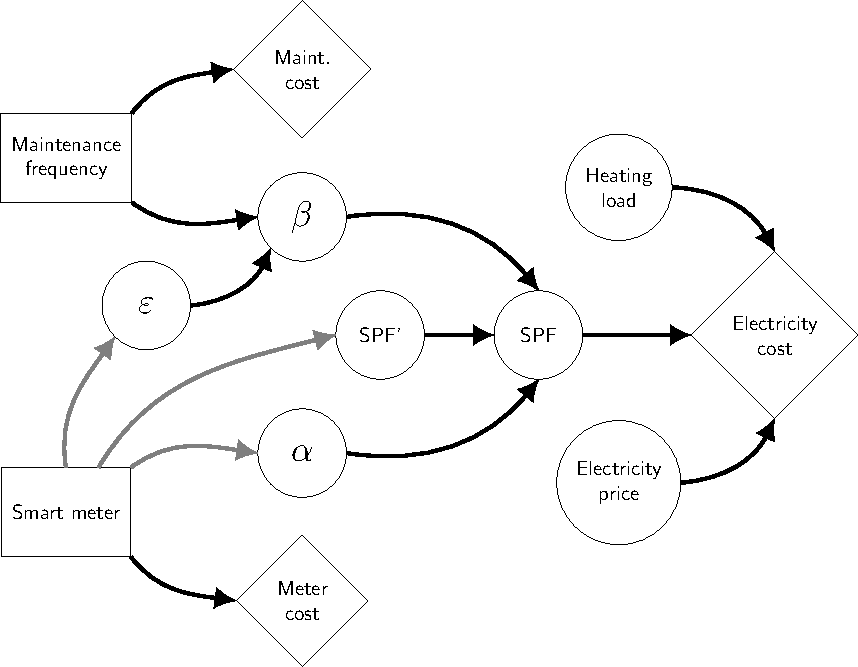
\includegraphics[width=0.75\linewidth]{ASHP-ID.pdf}
    \vspace{2pt}
    \caption{Influence diagram representation of \glsxtrshort{ashp} maintenance scheduling decision problem}
    \label{fig:ID-ASHP-maintenance}
\end{figure}

\newpage
Solving the Prior decision problem\footnote{\label{fn:pdp-defn} Refer back to \Cref{sec:methodology-bayesian-decision-analysis} for definition.}, the optimal maintenance frequency is found to be 2 activities per year, leading to an expected operating cost (Eq. \ref{eq:ASHP-total-cost}) of £1,876,300/year for the building heating system, of which £36,000/year (2\%) is spent on maintenance. Fig. \ref{fig:ASHP-prior-dist} plots the probability distribution of operational costs for the system when maintained 2 times a year. It demonstrates the significance of the uncertainties in the building energy system on the planning problem, as the cost of operating the heating system can vary from £1m/year to £4m/year, and so highlights the importance of accounting for those uncertainties during planning.

Solving the Pre-Posterior decision problem\footnoteref{fn:pdp-defn} with perfect information, i.e. planning maintenance with perfect knowledge of the uncertain parameters in the system, achieves an expected cost of £1,874,640/year. Therefore the Expected Value of Perfect Information (\glsxtrshort{evpi}), as defined in \Cref{sec:methodology-voi}, is £1,660/year.

Fig. \ref{fig:ASHP-post-action-freqs} shows the distribution of optimal maintenance frequency when the true values of the uncertain system parameters are known. In slightly over half of cases, perfect information about the system does not change the maintenance scheduling decision, i.e. the true solution is the same as the prior solution, indicated by the black column. However the information provides value, as in many cases the performance degradation of the \glsxtrshort{ashp}s is less severe, with less frequent maintenance providing lower operational cost. Monitoring information allows the system operator to avoid the cost of unnecessary maintenance activities in these cases.\\

\begin{figure}[h]
    \centering
    \begin{minipage}{.475\textwidth}
        \centering
        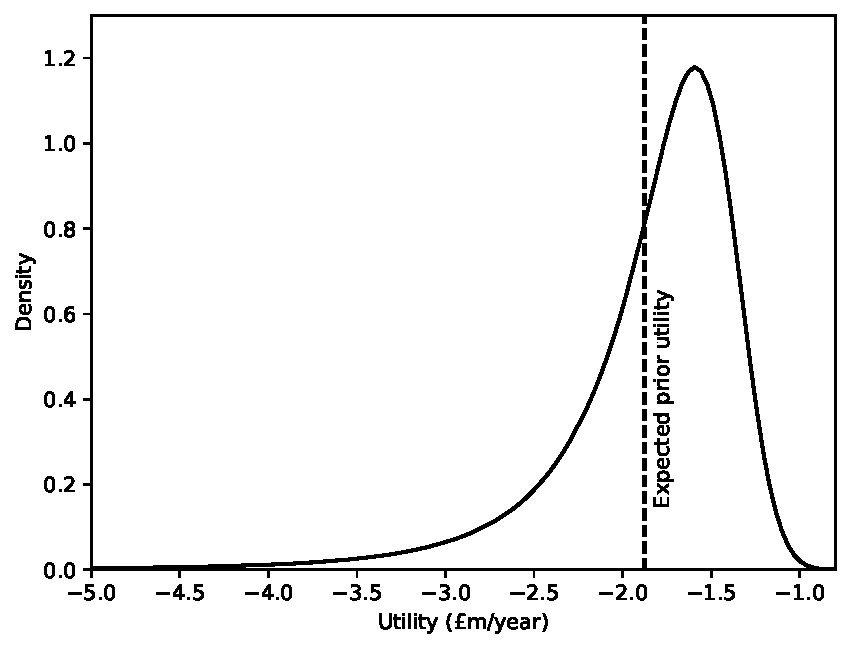
\includegraphics[width=\linewidth]{ASHP_prior_utility_distribution.pdf}
        \caption{Distribution of utilities achieved by optimal prior action, ${N_m}^*=2$. Dashed line indicates mean of distribution}
        \label{fig:ASHP-prior-dist}
    \end{minipage}%
    \hfill
    \begin{minipage}{.475\textwidth}
        \centering
        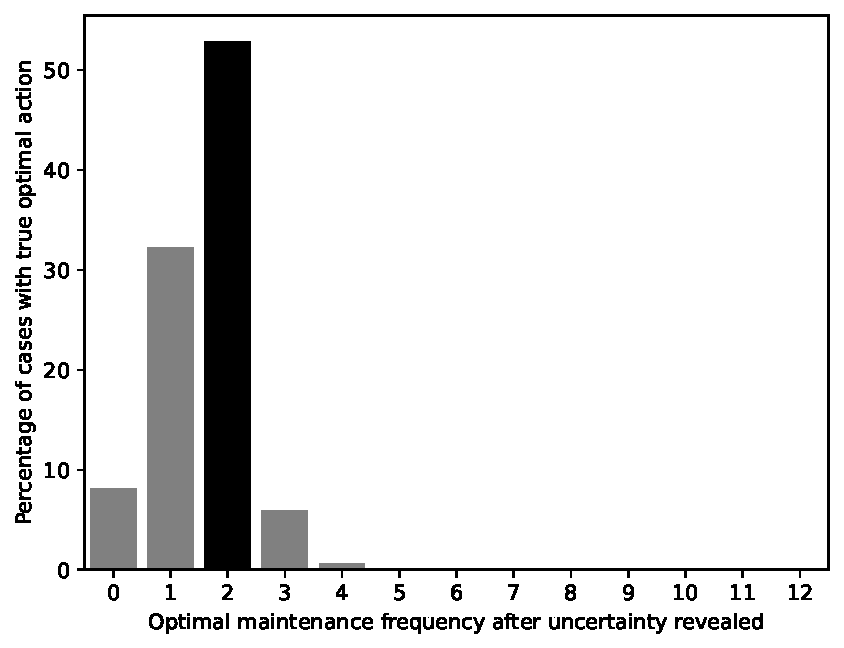
\includegraphics[width=\linewidth]{ASHP_posterior_action_freqs.pdf}
        \caption{Distribution of true optimal maintenance frequency, i.e. best action once uncertainty has been revealed}
    \label{fig:ASHP-post-action-freqs}
    \end{minipage}%
\end{figure}

\newpage
The annualised cost of the electricity smart meter used to monitor the \glsxtrshort{ashp} units (`meter cost' in Fig. \ref{fig:ID-ASHP-maintenance}) is estimated to be £70/year \citep{daikin2022DaikinUKPrice}. Therefore, the installation of smart meters capable of perfectly measuring \glsxtrshort{ashp} performance, degradation, and building load, and the dynamic scheduling of maintenance activities using the actual electricity price, would lead to a net economic benefit, \glsxtrshort{voi} minus information cost, of £1,590/year to the asset owner from reduced operational costs. In this way, the asset owner can justify their investment in smart meters.
% Or, conclude that: 1. this is very small c.f. the total operational cost, 2. true VoI is smaller, 3. this is only hardware cost (?) - so overall, probably not worth installing smart meters
The value of information provided by smart meters in this scenario is small compared to the total operational costs, only 0.06\%. However, the use of smart meters to optimise maintenance scheduling can provide additional benefits, such as extending the lifespan of the \glsxtrshort{ashp} units and decreasing the probability of malfunctions. These cost savings, although not accounted for in these calculations due to simplification, could be significant.\\


%%% Ventilation %%%
\section[Office ventilation scheduling]{Building occupancy measurement for real-time ventilation scheduling to improve indoor air quality} \label{sec:vent}

In mechanically ventilated office spaces, building managers must schedule ventilation system settings to ensure sufficient indoor air quality for the occupants. Adequate ventilation is required to prevent the transmission of airborne infectious diseases such as the SARS-CoV-2 virus (COVID-19), which is both damaging to the health of the occupants and costly for the tenant of the office space through lost productivity. However, operating ventilation at an unnecessarily high rate can impact occupant thermal comfort, lead to excessive carbon emissions, as well as excessive operational cost of the ventilation system through the additional heating/cooling demand required to condition air intake. The risk of viral transmission, and thus the appropriate ventilation setting, is highly dependent on the number of occupants in the office space. However, in the absence of occupant monitoring and dynamic ventilation control systems, building managers must schedule ventilation system settings without knowledge of the exact occupancy level of the space. At the time of deciding ventilation scheduling, the occupancy of the ventilated space over the operation period is uncertain. This uncertainty is particularly relevant in light of recent trends towards `work from home', which reduces the predictability of office occupancy.

This raises the question, ``Would it be worth installing a smart occupancy monitoring and ventilation control system in an office space to improve ventilation scheduling?'', i.e. would the economic benefit of improved ventilation control be greater than the cost of installing such a smart monitoring and control system?\\

A simple model of indoor air quality in a typical office space is considered. Said office space is taken to have a maximum occupancy of 100 people, a floor area of 1,000 m$^2$, and a ceiling height of 2.4 m. There are five available ventilation settings: 1, 3, 6, 12, and 20 air changes per hour (ACH). The ventilation system is assumed to have a fan of specific power 1.9 W/l/s, $P_{\text{fan}}$, operating at 60\% efficiency, $\eta$, for 10 hours per day, $T$. At an electricity unit price of 32.6 p/kWh, $p_e$, the cost of operating the ventilation system\footnote{The cost of heating/cooling associated with ventilation is neglected for simplicity, but can be readily added to the model.} at each setting is calculated as,
\begin{equation}
    C_{\text{vent}} = \text{ACH} \times V \times \frac{P_{\text{fan}}}{\eta} \times T \times p_e
\end{equation}
where $V$ is the volume of the office in litres, $T$ is expressed in seconds and $p_e$ in £/Wh.

A model of the probability of viral infection for an individual in an indoor space as described in \citep{deoliveira2021EvolutionSprayAerosol} is used, which is also available in web application form at \href{https://airborne.cam/}{\nolinkurl{airborne.cam}} \citep{gkantonas2021AirborneCamRisk}. It is assumed that the base prevalence of infection amongst the occupants is that of the general UK population in February of 2023, 2.18\% \citep{ons2023CoronavirusCOVID19Latest}, and that infection of an individual leads to 3 days of sick leave, which taking the median daily salary for full-time employees in 2022, costs the tenant £128/day \citep{ons2022EmployeeEarningsUK} in lost productivity.
It is further assumed that any occupants are present in the office space for the whole 8 hour work day, that time coupling effects between days can be neglected, i.e. that the model for a single day is representative, and so illness costs are calculated using the expected number of infections for the given occupancy. The prior distribution of occupancy is taken to be discrete uniform in the interval 0 to 100 inclusive.

The stochastic decision problem is thus to select the ventilation system setting which minimises the sum of the ventilation system operation (electricity) cost, and the cost of lost productivity due to illness to the tenant, subject to uncertainty in the occupancy level of the space.
\begin{equation}
    C_{\text{total}} = C_{\text{vent}}(\text{ACH}) + n \times p_{\text{infection}}(n,\text{ACH})
\end{equation}
where $n$ is the number of occupants in the office.

This decision problem can be described via the influence diagram provided in Fig. \ref{fig:ID-building-vent}.\\

\begin{figure}[p]
    \centering
    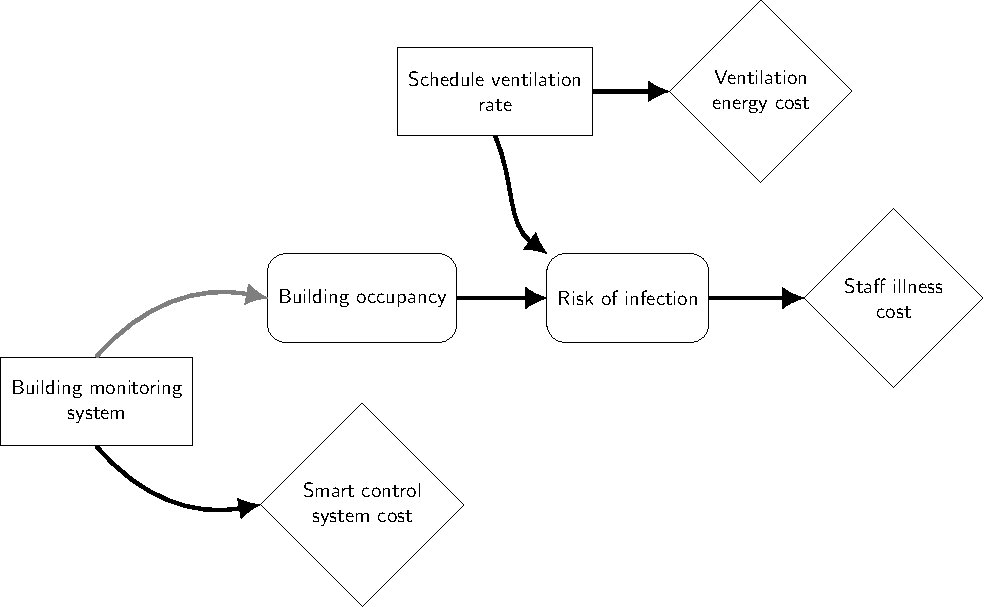
\includegraphics[width=0.66\linewidth]{building-vent-ID.pdf}
    \vspace{4pt}
    \caption{Influence diagram representation of building ventilation scheduling decision problem} \label{fig:ID-building-vent}
\end{figure}

\begin{figure}[p]
    \centering
    \begin{minipage}{.475\textwidth}
        \centering
        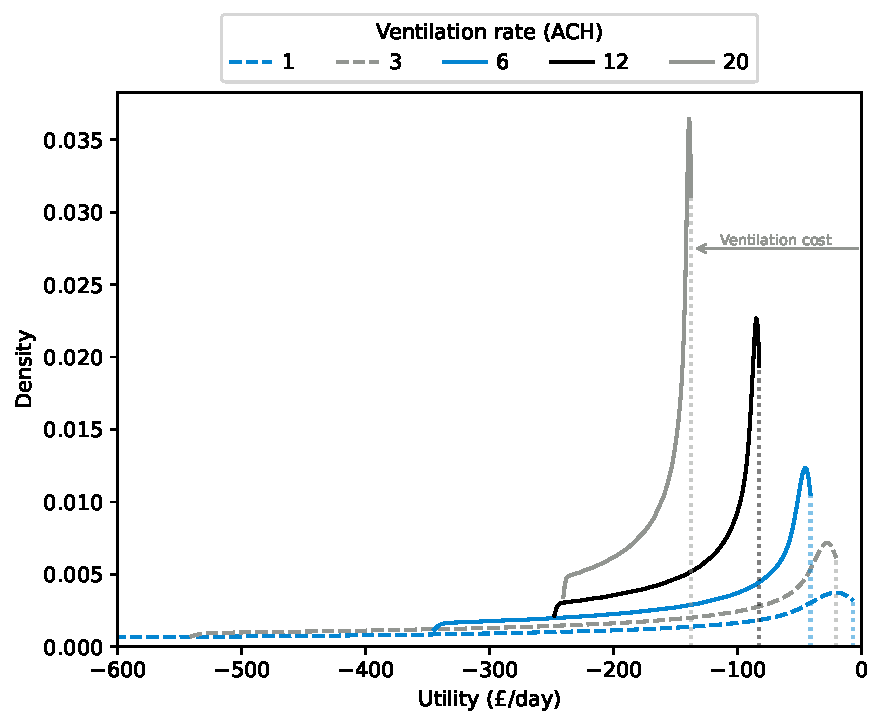
\includegraphics[width=0.975\linewidth]{building_vent_prior_u_dists_by_action.pdf}
        \caption{Distribution of utilities achieved by each ventilation rate under prior uncertainty}
        \label{fig:b_vent_a_dists}
    \end{minipage}%
    \hfill
    \begin{minipage}{.475\textwidth}
        \centering
        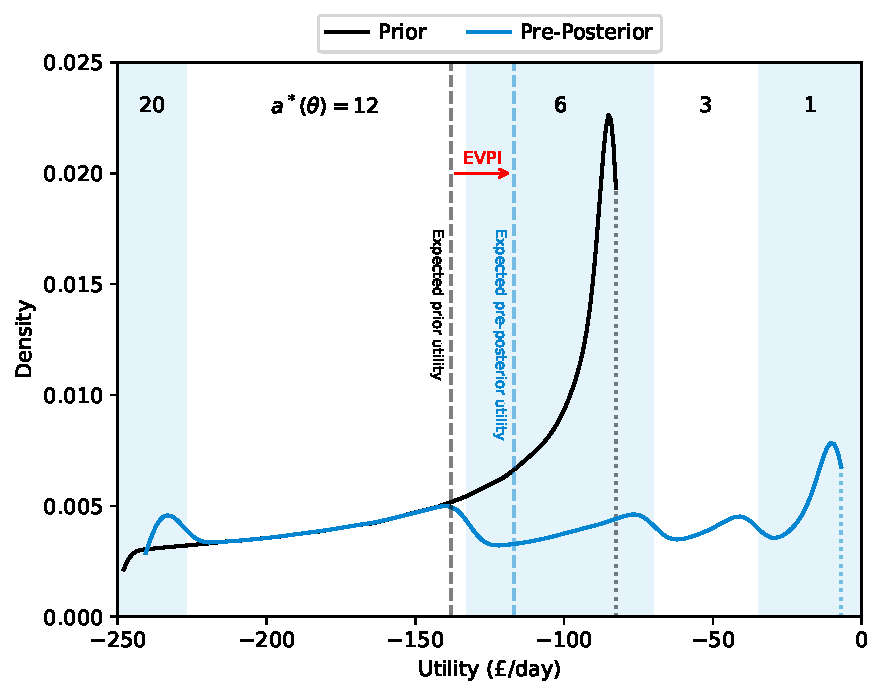
\includegraphics[width=0.95\linewidth]{building_vent_dists_prior_vs_pre_post.pdf}
        \caption{Distribution of utilities achieved by prior and pre-posterior decisions}
    \label{fig:b_vent_prior_vs_prepost}
    \end{minipage}%
\end{figure}

\begin{figure}[p]
    \centering
    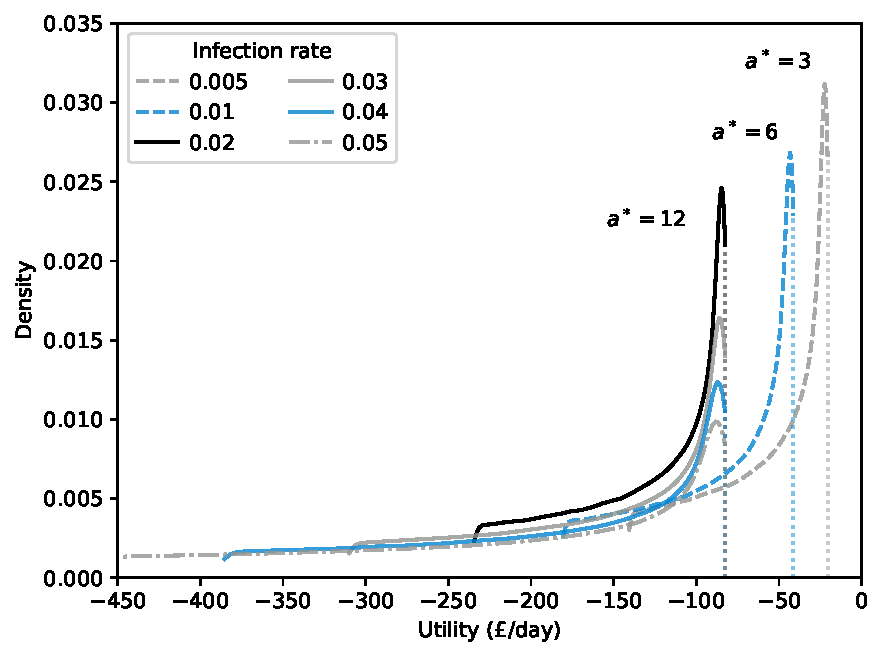
\includegraphics[width=0.45\linewidth]{building_vent_prior_u_dists_with_InfRate.pdf}
    \caption{Distributions of utilities for prior solution with varying assumed infection rate} \label{fig:b_vent_sensitivity}
\end{figure}

Solving the Prior decision problem, the optimal ventilation rate is found to be 12 air changes per hour, leading to an expected overall cost of £138/day for the tenant. Fig. \ref{fig:b_vent_a_dists} shows the distribution of utilities for each available ventilation rate under the prior uncertainty. Increasing the ventilation rate increases the base cost of all outcomes, indicated by the dashed line showing the minimum cost for each curve, but reduces the risk of large numbers of infections occurring when the office has high occupancy, limiting the maximum cost. The utility distribution for the prior optimal ventilation rate of 12 ACH in the base case is indicated by the black curve in Figures \ref{fig:b_vent_a_dists} to \ref{fig:b_vent_sensitivity}.
% discuss risk vs mean reward trade-off??

Solving the Pre-Posterior decision problem with perfect information, i.e. dynamically scheduling ventilation with perfect knowledge of occupancy from a monitoring system, achieves an expected cost of £117/day. Therefore, the \glsxtrshort{evpi} is £21/day. Hence, over a 20 year operational lifetime, the smart monitoring and control system could save the tenant up to £850,000, or 15\% of the total operating cost. Fig. \ref{fig:b_vent_prior_vs_prepost} plots the distribution of utilities achieved by the prior and pre-posterior decisions. For the prior, the same decision of 12 ACH is used in all cases as no measurement is taken. Whereas, for the pre-posterior, the ventilation rate is set using information on the occupancy level in each case. The blue regions indicate the regime of cases where each ventilation rate is selected by the pre-posterior decision, i.e. where it is the lowest cost choice. The pre-posterior density is similar to the prior in the region of high costs, but is much more uniform and extends substantially further into the low cost region, indicating that the \glsxtrshort{voi} is primarily derived from the ability to reduce ventilation rate and save electricity cost when office occupancy is low.

Building managers can use the computed \glsxtrshort{evpi} to support their decision making about whether investment in smart occupancy monitoring and ventilation control systems are worthwhile. If a proposed smart monitoring and control system is expected to have an installation and maintenance cost over the 20 year lifetime of more than £850,000, then this investment will not be beneficial for the context of ventilation scheduling. A cheaper but less precise method of estimating occupancy, such as a desk booking system, may be a more suitable strategy, or it may be most cost effective to forego occupancy measurement altogether and use a fixed ventilation rate.

%% Sensitivity analysis, discuss implications
\subsection*{Sensitivity analysis}
The problem formulation considered assumes a variety of properties about the office being ventilated. However, commercial building stocks are diverse, and the actual value of these properties varies between buildings. A sensitivity analysis is performed to investigate whether occupancy monitoring and dynamic ventilation scheduling remains valuable across different sized offices. The \glsxtrshort{voi} analysis is repeated for office models with 5 to 25 m$^2$ of floor area per person, maintaining a maximum occupancy of 100, and keeping all other properties as before. Table \ref{tab:floor-area-sensitivity} provides the optimal ventilation rate without measurement and the \glsxtrshort{evpi} for each size of office considered. The \glsxtrshort{evpi} is lowest in the extreme cases where extreme ventilation rates are optimal both on average (for the prior problem) for the majority of occupancy outcomes. For instance, in the smallest office, the highest available ventilation rate of 20 ACH is the optimal prior decision, and the optimal decision for 53\% of occupancy outcomes. For all office sizes tested, the \glsxtrshort{evpi} remains significant, 10\% or more of the prior expected cost, suggesting that occupancy monitoring systems are likely beneficial for offices of any size.\\

\begin{table}[h]
    \centering
    \renewcommand{\arraystretch}{1}
    \begin{tabular}{c|ccccc} \toprule \toprule
        Floor area per person (m$^2$) & \: 5 \: & \: 10 \: & \: 15 \: & \: 20 \: & \: 25 \: \\ \midrule
        Prior optimal ventilation rate (ACH) & 20 & 12 & 6 & 3 & 3 \\
        \glsxtrshort{evpi} (£/day) & 14 & 21 & 16 & 19 & 14 \\
        \bottomrule \bottomrule
    \end{tabular}
    \smallskip
    \caption{Sensitivity of prior solution and \glsxtrshort{evpi} to office size}
    \label{tab:floor-area-sensitivity}
\end{table}

The prevalence of viral illness in the general population has a significant impact on the risk of infection spreading in an office environment, and so should be taken into account by a building manager when setting ventilation rates, and as a result when determining what information is required to support that decision. The sensitivity of the prior decision and \glsxtrshort{evpi} is tested for infection rates from 0.5\% to 5\% \citep{ons2023CoronavirusCOVID19Latest}. Table \ref{tab:inf-rate-sensitivity} provides the results of this analysis, and Fig. \ref{fig:b_vent_sensitivity} plots the distribution of utilities for the prior solutions at each infection rate. As infection rate increases, the risk of infection at a given occupancy level rises, causing a widening of the utility distribution, and so greater risk for the decision maker. Additionally, the distribution of true optimal ventilation rates flattens. Hence, for more occupancy outcomes a different ventilation rate to the prior is optimal, and the benefit of that improved decision increases. Therefore, the greater the infection rate, the higher the \glsxtrshort{voi}, and the more valuable occupancy monitoring becomes. The sharp increase in \glsxtrshort{evpi} between infection rates of 1\% and 2\% highlights the importance of using sensitivity analysis to determine whether conclusions about the economic benefits of data collection derived from \glsxtrshort{voi} analysis remain valid as assumptions about the studied building energy system are varied. Alternatively, assumed parameters can be modelled as uncertainties and included within the system model.\\

\begin{table}[h]
    \centering
    \renewcommand{\arraystretch}{1}
    \begin{tabular}{c|cccccc} \toprule \toprule
        Infection rate (\%) & 0.5 & 1 & 2 & 3 & 4 & 5 \\ \midrule
        Prior optimal ventilation rate (ACH) & 3 & 6 & 12 & 12 & 12 & 12 \\
        \glsxtrshort{evpi} (£/day) & 8 & 11 & 22 & 21 & 24 & 30 \\
        \bottomrule \bottomrule
    \end{tabular}
    \smallskip
    \caption{Sensitivity of prior solution and \glsxtrshort{evpi} to infection prevalence in the population}
    \label{tab:inf-rate-sensitivity}
\end{table}


%%% GSHP %%%
\section[\glsxtrshort{gshp} borehole design]{Ground conductivity measurement for optimising borehole design in residential ground source heat pump heat supply systems} \label{sec:gshp}

\glsxtrlong{gshp} (\glsxtrshort{gshp}) systems use the ground as a source and sink of heat to provide cooling and heating for buildings in a highly energy efficient way \citep{aresti2018ReviewDesignAspects}. As these systems exchange heat with the ground, their performance (characterised by the \glsxtrshort{cop}s they achieve) is influenced significantly by the geological properties of the ground with which they exchange heat. In the design of such \glsxtrshort{gshp} heating \& cooling supply systems, it is desired to match the capacity of the \glsxtrshort{gshp} system to energy demand of the building as to minimise the overall cost of operating the supply system over its lifetime. The overall operating cost is composed of the capital cost of constructing the system, and the operational costs, which are primarily the cost of the electricity required to meet the building energy demands. Under-specification of the systems leads to greater electricity usage from less efficient and so higher cost auxiliary heating systems, whilst over-specification of the system results in unnecessary capital cost.

At the time of system design, the thermal properties of the ground are typically not known precisely, as existing geological survey data provides an uncertain estimate of the ground properties in the site location \citep{dallasanta2020UpdatedGroundThermal}. However, the system designer has the option to commission thermal tests at the site location prior to designing the \glsxtrshort{gshp} system. Whilst these tests reduce the uncertainty in the ground thermal properties, they are time-consuming and incur additional costs. As a result, these tests are often not conducted, and generally available information on materials and location is used to provide uncertain estimates of ground thermal properties which are used to design the \glsxtrshort{gshp} system. This therefore poses the following question to the designer, ``Would commissioning thermal tests reduce the overall lifetime cost of the \glsxtrshort{gshp} heat supply system by improving the matching of the designed system capacity to the building load?''.\\

A simplified \glsxtrshort{gshp} system design task for a residential building heat supply system is considered. In this design task, the designer must select the length of boreholes, $L_{\text{bh}}$, to be drilled for the ground heat exchange. The available length choices are 110 to 190 m, in 5 m increments. The capital cost of borehole drilling is taken to be 70 £/m/borehole.

It is assumed that the effective ground thermal conductivity, $\lambda_{\text{ground}}$, is the only uncertain geological parameter, and that it is Normally distributed with mean 1.94 W/mK, and standard deviation 0.31 W/mK,
\begin{equation}
    \lambda_{\text{ground}} \sim \mathcal{N}(\mu=1.94,\sigma=0.31) \:\: \text{W/mK}
\end{equation}
which is the average thermal conductivity over the range of borehole depths considered, and covers typical uncertainty ranges given the heterogeneity present in soils \citep{busby2018ModellingStudyVariation,busby2011ProvisionThermalProperties,loveridge2013ThermalResponseTesting}.

The designed \glsxtrshort{gshp} system, consisting of 12 boreholes, must supply heat to a small apartment block of 10 flats over a 50 year operational lifetime. The building is assumed to have a typical heating demand distribution for its type, and a simplified load profile is synthesised based on demand values for the UK \citep{mitchell2020UKPassivhausEnergy}, and using historic weather data for London. This synthetic load profile, $E_{\text{load}}(t)$, consumes 116MWh/year, corresponding to a 13.2 kW mean heating load for the building, with a peak load power of 30.5 kW. The data can be found in the \href{https://github.com/EECi/VOI-for-Building-Energy}{GitHub repository}.

The model of geothermal borehole operation presented in \citep{lamarche2007NewContributionFinite} is used to determine the scheduling of energy extracted from the ground in each time instance, $E_g(t)$, with the borehole fluid temperature, $T_{\text{fluid}}$, conservatively constrained to be within the range $5$ degC to $35$ degC,
\begin{equation}
    5 \leq T_{\text{fluid}}(t) \leq 35
\end{equation}
In this model, $T_{\text{fluid}}$ is a function of the power extracted from the ground, $E_g(t)$, the ground thermal conductivity, $\lambda_{\text{ground}}$, the borehole length, $L_{\text{bh}}$, and the other assumed ground condition parameters.

Given the fluid temperature schedule determined, the instantaneous \glsxtrshort{cop} of the \glsxtrshort{gshp} system is computed using the following empirical relationship from \citep{kensa2014HowCOPVaries},
\begin{equation}
    \text{COP}(t) = 4.0279 +0.1319 \cdot T_{\text{fluid}}(t)
\end{equation}
The energy that is provided by the \glsxtrshort{gshp} system to the building is then given by,
\begin{equation}
    E_{\text{GSHP}}(t) = \frac{E_g(t)}{1-1/\text{COP}(t)}
\end{equation}
If the \glsxtrshort{gshp} system is unable to meet the building load in any time instance, the remaining unsatisfied load is provided by an auxiliary heat supply system with a \glsxtrshort{cop} of 1.
\begin{equation}
    E_{\text{load}}(t) = E_{\text{GSHP}}(t) + E_{\text{aux}}(t)
\end{equation}
The total electricity consumption of the combined heat supply system is therefore given by,
\begin{equation}
    e_{\text{total}} = \sum_t \left( \frac{E_{\text{GSHP}}(t)}{\text{COP}(t)} + E_{\text{aux}}(t) \right)
\end{equation}
The cost of electricity used by the residential building is taken to be 32.6 p/kWh.

The stochastic decision problem of designing borehole lengths as to minimise the expected lifetime cost of the heating supply system is represented as an influence diagram in Fig. \ref{fig:ID-GSHP-design}.\\

\begin{figure}[h]
    \centering
    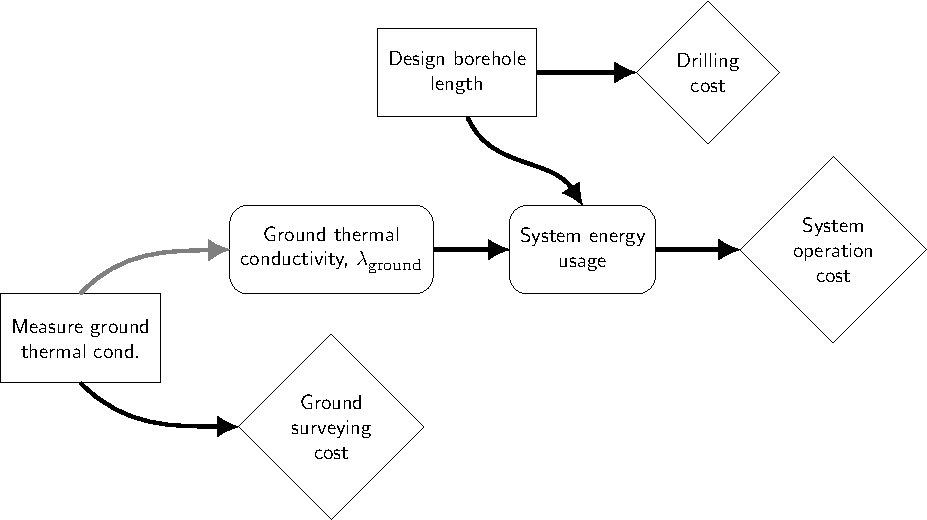
\includegraphics[width=0.8\linewidth]{GSHP-design.pdf}
    \vspace{4pt}
    \caption{Influence diagram representation of \glsxtrshort{gshp} heat supply system design decision problem}
    \label{fig:ID-GSHP-design}
\end{figure}

Solving the Prior decision problem, the optimal borehole length is found to be 155 m, leading to an expected overall lifetime cost of £819,100 for the heating system.

Various technologies exist for measuring ground thermal properties. Table \ref{tab:ground-tests} presents the cost and experimental uncertainty of thermal probe tests and Thermal Response Tests (TRT),  which are commonly used for ground thermal conductivity measurement. The extended TRT measurement is a hypothesised base case for the results achievable with TRT methods. The likelihood of obtaining a measurement $z$ for each test given a true underlying ground thermal conductivity of $\lambda$ is modelled using a Gaussian distribution as,
\begin{equation}
    f_e(z|\lambda) \sim \mathcal{N} \left( z,0,\frac{\nu_e}{2} \lambda \right)
\end{equation}
where $\nu_e$ is the decimal experimental uncertainty of the test.
% Mention that we use Stan to sample from the posterior - as it's quite complicated

\begin{table}[h]
    \centering
    \renewcommand{\arraystretch}{1}
    \begin{tabular}{c|c|c|c} \toprule \toprule
        Method & Uncertainty & Cost (£) & References \\ \midrule
        Thermal probe (in situ) & 25\% & 187 & {\footnotesize \citep{king2012FieldDeterminationShallow}, \citep{sunbeltrentals2023ThermtestTLS100Thermal}} \\
        Thermal probe (lab test) & 17\% & 1,800 & {\footnotesize \citep{low2013MeasuringSoilThermal}, \citep{basaltridgetestinglaboratory2024BasaltRidgeTesting}} \\
        Thermal Response Test (TRT) & 10\% & 5,000 & \makecell{\footnotesize \citep{choi2021DevelopmentChillerattachedApparatus},\\[-.5ex] \footnotesize\citep{spitler2000SituMeasurementGround},\\[-.5ex] \footnotesize\citep{tang2019SensitiveAnalysisEffective}} \\
        Extended TRT & 5\% & 10,000 & -- \\
        \bottomrule \bottomrule
    \end{tabular}
    \smallskip
    \caption{Uncertainty and cost of ground thermal conductivity measurement tests}
    \label{tab:ground-tests}
\end{table}

The \glsxtrlong{evii} (\glsxtrshort{evii}) is computed for each available test, which is compared to the associated cost to determine the net benefit to decision making provided. Fig. \ref{fig:GSHP-EVIIs} plots the results. All tests provide significant net benefit to the heating system design task, indicating that site specific ground thermal testing should be conducted prior to the design of \glsxtrshort{gshp} based heating systems. The TRT provides the greatest net added value to the decision maker, and so using this \glsxtrshort{voi} analysis, the designer of this energy system can justify and optimise their expenditure on ground testing to support their decision making. This demonstrates that additional uncertainty reduction through more data collection or more precise measurement does not always provide sufficient improvements to decision making to warrant its cost.\\

\begin{figure}[h]
    \vspace*{-0.5cm}
    \centering
    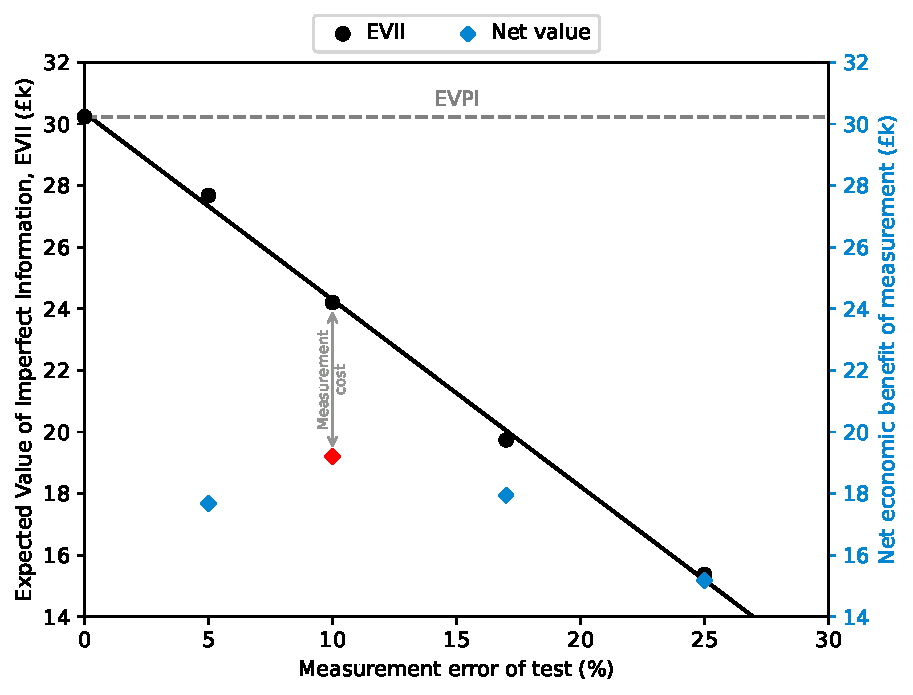
\includegraphics[width=0.8\linewidth]{GSHP_EVIIs.pdf}
    \vspace*{-0.2cm}
    \caption{\glsxtrlong{evii} (\glsxtrshort{evii}) and net economic benefit (\glsxtrshort{evii} minus measurement cost) of imprecise ground thermal conductivity measurements}
    \label{fig:GSHP-EVIIs}
\end{figure}


\newpage
%********************************** Conclusions **************************************
\section{Conclusions} \label{sec:demonstrations-conclusions}

This chapter demonstrated how \glsxtrshort{voi} can be used to quantify the benefit of data collection to support decision making in building energy systems, and as a decision support tool for evaluating data collection strategies. Three example decision problems covering the management, operation, and design of building energy systems were studied: heat pump maintenance scheduling, office ventilation scheduling, and ground source heat pump system design.

% ASHP maintenance
Installing smart meters in \glsxtrshort{ashp}s for dynamic maintenance scheduling was found to be a worthwhile investment. However, improvements in decision making provided were extremely limited, with perfect knowledge of heat pump condition leading to only a 0.06\% reduction in operational costs on average.
% Office ventilation
Occupancy monitoring systems enabled significant cost savings when scheduling ventilation to manage indoor air quality and infection risk in office spaces, reducing the total cost to the tenant by 10.2-16.4\%. Occupancy information was found to be more valuable in mid-sized offices and when infection is more prevalent, e.g. in the winter.
% GSHP design
When designing a \glsxtrshort{gshp} based heating system for a block of flats, ground thermal tests to reduce uncertainty in thermal conductivity were found to be beneficial to support system design. A Thermal Response Test (TRT) was determined to be the optimal data collection strategy, enabling net savings of £19k on the lifetime cost of the heating system.

In each example problem a different capability of the \glsxtrshort{voi} framework was demonstrated: the ability to simply and clearly represent and analyse decisions in complex engineering systems, the identification of system characteristics for which data collection is worthwhile, and the determination of optimal data collection strategies when trading-off measurement precision versus cost.

The examples in this chapter show that \glsxtrlong{voi} analysis gives a clear and principled methodology for addressing the current research gap of quantifying the benefit of data collection to support decision making in the building energy systems literature. It provides a route to rationalise data collection strategies and avoid resource wastage on low insight data as building digitisation progresses. However, these examples use significantly simplified models of how decisions are made in building energy systems, and don't got into much depth about how the uncertainty reduction that the data provides affects the decision making process.
\cleardoublepage
%!TEX root = ../thesis.tex
%*******************************************************************************
%*********************************** Forecasting chapter *****************************
%*******************************************************************************

\chapter[Forecasting data requirements for \glsxtrshort{mpc}]{Data requirements of load forecasting for model predictive control} \label{chap:forecasting}

\graphicspath{{Forecasting/Figs/}}

\begin{cbox}{}
    \printpublication{langtry2024ImpactDataForecasting}

    \noindent{\color{black!50}\rule{\textwidth}{0.4mm}}\vspace{2mm}

    \noindent
    This chapter has been published as the journal article above. The co-authors of this article developed the code for the simple neural models used in the experiments. They also performed the data similarity metric and change-point analyses, detailed in Appendices \ref{app:forecasting-similarity-metric} \& \ref{app:forecasting-change-points}, and the data feature and online training experiments in Section \ref{sec:forecasting-data-efficiency}, providing a small amount of the text describing these analyses. Other than these contributions, all of the code, analysis, and text in this chapter is my own work.
\end{cbox}

\begin{cbox}{}
    All code and data used to perform the experiments in this chapter is available at \url{https://github.com/EECi/Annex_37}.
\end{cbox}

\hfill \\

%********************************** Graphical abstract **************************************
\begin{figure}[h]
    \centering
    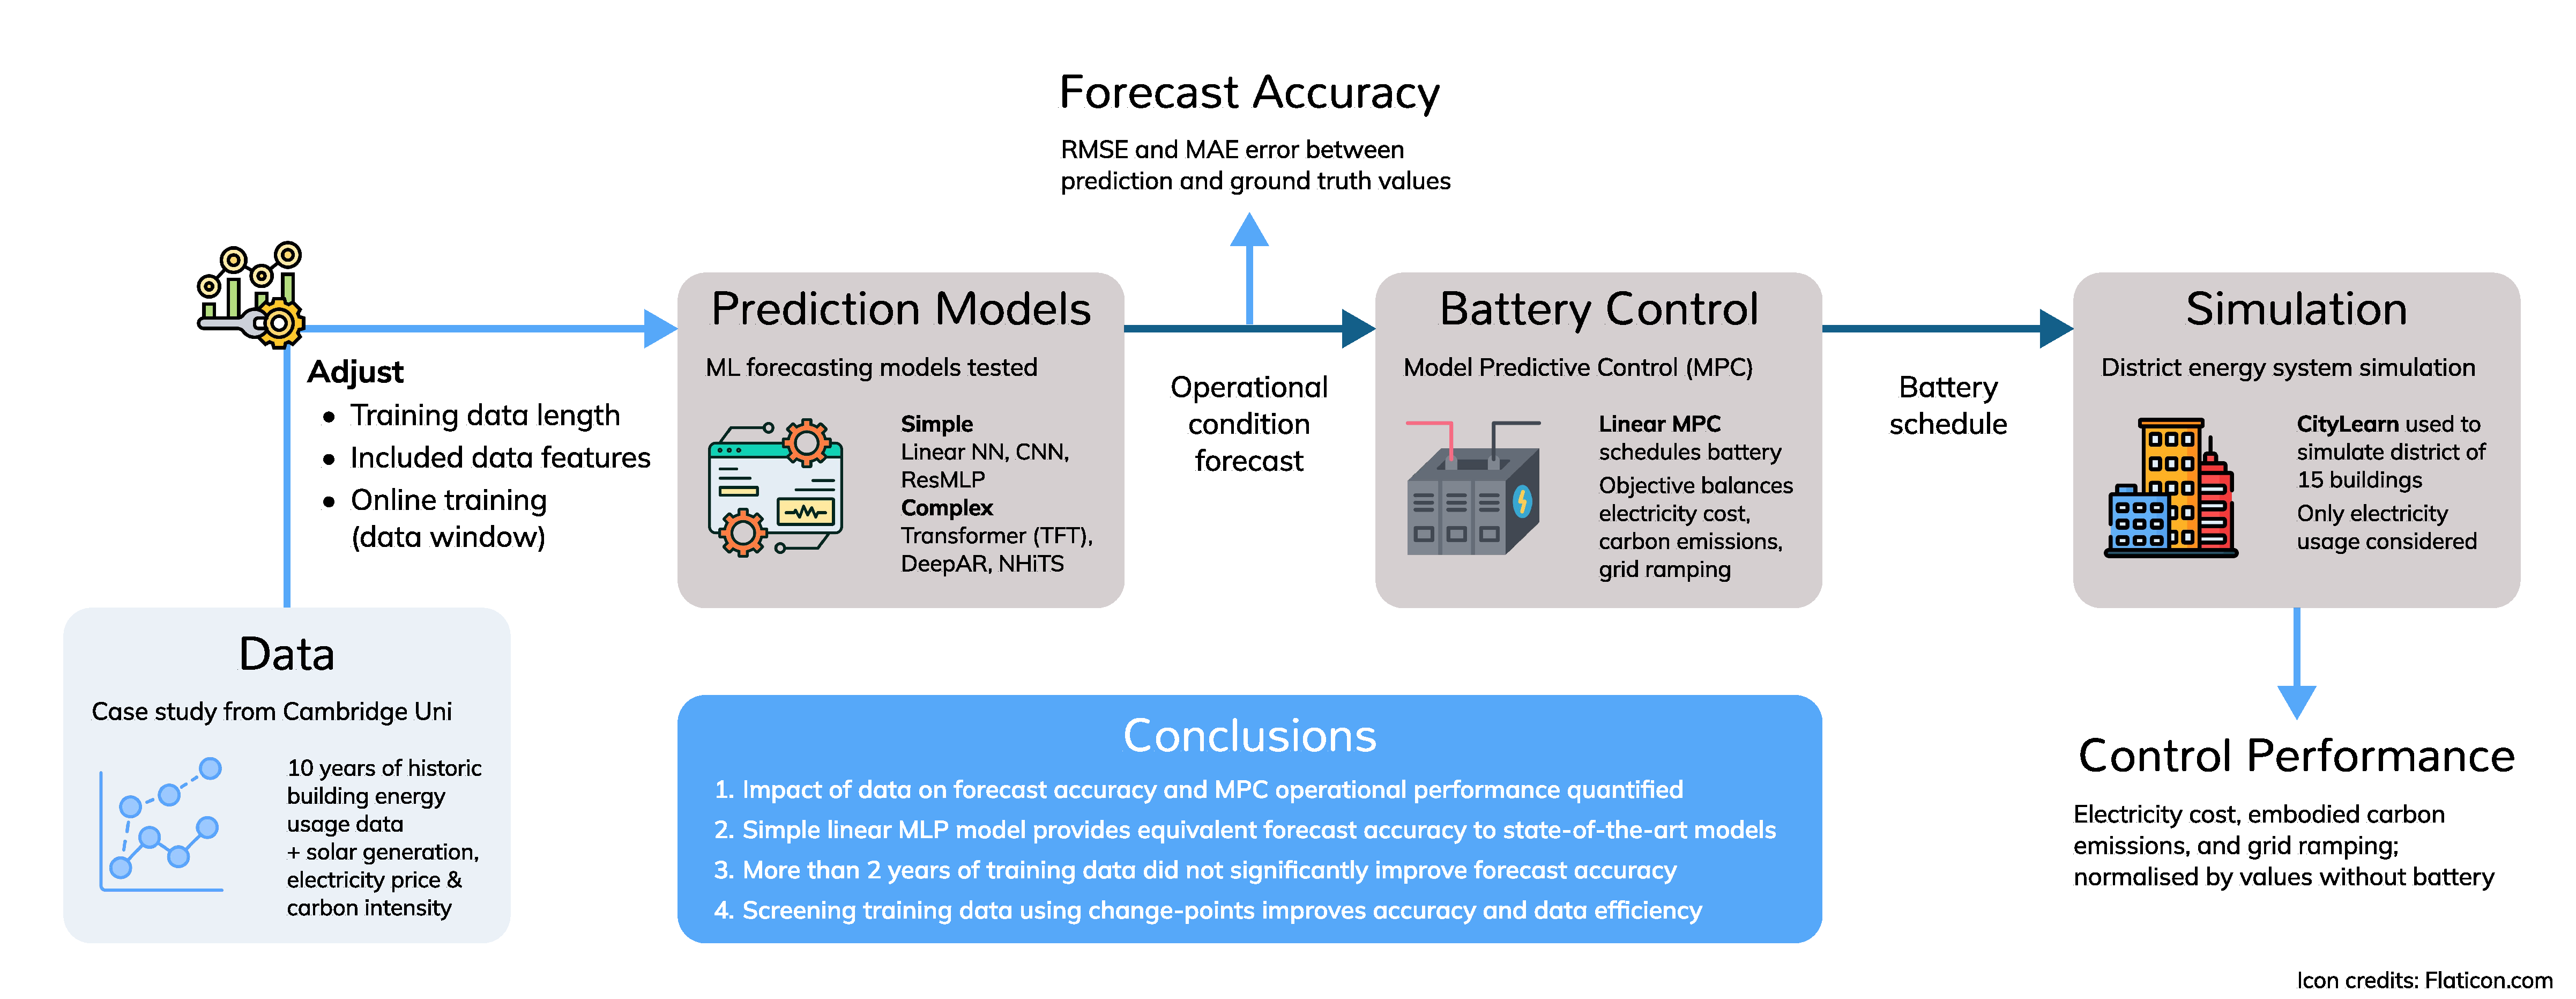
\includegraphics[width=\textwidth]{Graphical_Abstract.pdf}
    \caption{Graphical abstract of \Cref{chap:forecasting}.}
    \label{fig:forecasting-forecasting_graphical_abstract}
\end{figure}
\hfill \\
%********************************** end **************************************

\vspace{0.5cm}

\noindent
Data is needed to develop forecasting models for building behaviour that are used for smart control of the building energy systems to reduce the cost and carbon emissions of building operation. However, this data is costly to both collect and exploit. Determining the most cost effective data usage strategies and setting data collection requirements for these systems requires understanding of how data affects forecast accuracy, and the resulting impact on the operational performance of the building control. This chapter investigates how the available data affects the forecasting accuracy of machine learning prediction models, and how the accuracy of these prediction models affects the performance of \glsxtrlong{mpc} in a simulated multi-building energy system. The data requirements of state-of-the-art and simple textbook machine learning models are compared, and measures to improve the data efficiency of these models are investigated. Specifically, reuse of prediction models, reduction of training data duration, reduction of model data features, and online model training.


\newpage
%********************************** Intro section **************************************
\section{Introduction}

Distributed generation and storage technologies, most commonly solar panels and batteries, are used to reduce the cost and or operational emissions building energy systems \citep{aminitoosi2022BuildingDecarbonizationAssessing,oshaughnessey2021DemandSideOpportunityRoles,zhu2023ReviewDistributedEnergy}. `Smart' operation of these energy storage systems can reduce the impact the building's energy usage has on the electrical grid, by allowing energy flexibility through demand-side management and demand response \citep{vazquez-canteli2020MARLISAMultiAgentReinforcement}. This is particularly important in light of the expected electrification of heating demands \citep{leibowicz2018OptimalDecarbonizationPathways}, and the peak load issues this will cause. The effectiveness of these systems, quantified by operational performance metrics of the building energy system such as total electricity cost, incurred carbon emissions, and measures of grid impact, is determined by the ability of the storage control scheme to arbitrage energy and alter the timing of net energy usage to meet these operational goals. As a result, lots of research effort has been put into developing performant storage control strategies in recent years \citep{drgona2020AllYouNeed,wang2020ReinforcementLearningBuilding,kathirgamanathan2021DatadrivenPredictiveControl}.

\glsxtrlong{mpc} (\glsxtrshort{mpc}) is one of the two leading control methodologies in the current building energy systems literature, alongside \glsxtrlong{rl} (\glsxtrshort{rl}). Its use in smart energy storage systems in buildings has been widely studied \citep{zhou2021IncorporatingDeepLearning,deng2023EvaluationDeployingDatadriven,souto2018ScenarioBasedDecentralizedMPC,touretzky2014IntegratingSchedulingControl,lee2020ModelPredictiveControl}, and it has been found to provide substantial operational performance improvements compared to \glsxtrlong{rbc} (\glsxtrshort{rbc}) \citep{lee2020ModelPredictiveControl,erfani2021AnalysisImpactPredictive,oldewurtel2012UseModelPredictive}, the main technology used in existing building systems. It has also been shown to provide comparable performance to \glsxtrshort{rl} based control \citep{zhan2023ComparingModelPredictive}. Review papers \citep{wang2022ScienceMappingApproach,thieblemont2017PredictiveControlStrategies,farrokhifar2021ModelPredictiveControl} provide a thorough overview of the applications of \glsxtrshort{mpc} to building energy systems with distributed generation and storage.

\glsxtrshort{mpc} requires a model of the system dynamics, which estimates the next state of the system given; (a) the current system state, (b) current operational conditions, and (c) the applied control actions. Using this dynamics model and forecasts of the operational conditions over a given planning horizon, it predicts the operation of the system over that planning horizon. Optimization techniques are then used to determine the set of control actions that optimize a specified objective over the planning horizon. The performance of \glsxtrshort{mpc} therefore depends on: the accuracy of the system dynamics model, the accuracy of the operational condition forecasts, the ability of the optimization method to identify near-optimal control actions, and the match between the objective over the planning horizon and the global operational goals of energy management for the system. This chapter focuses on the accuracy of operational condition forecasts, and its resulting impact on the operational performance of \glsxtrshort{mpc}. \citep{raisch2025AdaptingChangeComparison} explores how data affects the accuracy of the system dynamics model, building on previous work on the topic by the main author \citep{raisch2025GenTLGeneralTransfer}.


\subsection{Forecasting models for \glsxtrshort{mpc}}

Lots of different time series forecasting methodologies have been studied for the predicting operational conditions for building energy management \citep{sun2020ReviewThestateoftheartDatadriven}, however recent research has focused on machine learning based methods \citep{zhang2021ReviewMachineLearning,chou2018ForecastingEnergyConsumption,dai2023ComparisonDifferentDeep,rahman2018PredictingElectricityConsumption,fan2019AssessmentDeepRecurrent} due to their promising performance. Successes in other fields have prompted the investigation of large-scale, high-complexity model architectures \citep{choi2023PerformanceEvaluationDeep,dai2023CityTFTTemporalFusion}. However, there is doubt about whether such complex models are appropriate for use in the context of \glsxtrshort{mpc} for building energy systems \citep{zeng2023AreTransformersEffective,bunning2022PhysicsinformedLinearRegression,bunning2021ComparingMachineLearning}, due to the computational and data availability limitations in practical systems. So both simple and high-complexity, state-of-the-art machine learning forecasting models are investigated.


\subsection{Impact of data on forecast accuracy and \glsxtrshort{mpc} performance}

As machine learning methods are purely data-driven, `black box' prediction models, achieving accurate forecasts requires the availability of training data that is representative of the building energy system for which the model will be used. However, acquiring representative training data is both challenging and costly.
The costs of acquiring data include not only the capital costs of installing monitoring systems, but also the costs of digital infrastructure, data processing, system maintenance, and quality assurance required to support data collection. For the case of developing forecasting models for \glsxtrshort{mpc} considered in this study, there are additional project costs associated with delaying the installation of the battery system while data is gathered. \citep{motegi2003CaseStudiesEnergy} estimates the capital cost of electricity and gas smart-metering for a university campus to be \$0.27/m$^2$, plus an additional \$0.11/m$^2$ for maintenance and supporting IT systems. However, this considers only the cost of collecting data, and neglects the significant costs of training and deploying machine learning models \citep{strubell2020EnergyPolicyConsiderations}, from both the computing and expertise required.
Whilst the importance of data availability and the impact of data on forecast accuracy are widely acknowledged in the existing literature \citep{kathirgamanathan2021DatadrivenPredictiveControl,lee2020ModelPredictiveControl,wang2022ScienceMappingApproach,choi2023PerformanceEvaluationDeep,zhan2021DataRequirementsPerformance}, few works study the role of data in enabling good operational performance for \glsxtrshort{mpc} in building energy systems.

Determining cost optimal data collection strategies to support the development of forecasting models for \glsxtrshort{mpc} in buildings requires understanding of the trade-off between the quantity of data \& data features used for model training, and its associated costs, and the operational performance achieved by the controller. This impact of data for forecasting on \glsxtrshort{mpc} operational performance can be considered in two stages, by firstly studying the relationship between data and forecast accuracy of the resulting models, and then the sensitivity of the controller operational performance to the accuracy of forecasts.\\

Only a single previous study has investigated the impact of data on the accuracy of forecasting models for building energy management. This work, \citep{choi2023PerformanceEvaluationDeep}, compares the prediction accuracy of deep learning architectures for forecasting thermal loads and building zone temperatures over varying training dataset sizes. It finds that increasing the training data length does not always improve prediction accuracy due to the strong seasonality of building energy behaviours, but that the addition of data with good similarity to the test dataset into the training dataset greatly improves forecast accuracy. A limitation of this study is that it analyses only a single year of thermal load and zone temperature data, synthesised from a building energy model and historical weather data, meaning that a limited range of training dataset sizes, from 3 to 9 months, is considered. As a result, training data preceding the test data by one year, which due to seasonality is likely to have the highest similarity and so greatest value, is unavailable, meaning the study of the benefit of additional training data is incomplete.\\

The impact of forecast accuracy on \glsxtrshort{mpc} operational performance has been studied to a limited extent. \citep{erfani2021AnalysisImpactPredictive} compares the use of various classical and machine learning forecasting models in a common \glsxtrshort{mpc} framework, quantifying both the forecast accuracy and resulting operational performance of \glsxtrshort{mpc}. However, the models studied all achieve comparable forecast accuracies and operational performances, meaning limited insight can be gained into the relationship between the two. Further, as comparison is made between model types, these results cannot be used to assess the benefit of forecast improvement for any individual model.
\citep{oldewurtel2012UseModelPredictive} shows that the use of more accurate, external weather forecasts improves \glsxtrshort{mpc} operational performance, but does not quantify the forecast accuracies for comparison. In \citep{bartolucci2019HybridRenewableEnergy}, the prediction accuracy and corresponding operational performance of \glsxtrshort{mpc} for two forecasts of electrical load with different levels of synthetic noise are quantified. Finally, \citep{enriquez2016SolarForecastingRequirements} provides the most complete study, investigating the variation of operational performance with the noise amplitude of synthetic forecasts of temperature and solar irradiance. However, as the forecast accuracy of the synthetic predictions is not quantified, these results cannot be compared to the performance of practical prediction models and used to assess the benefits of forecast accuracy improvements.

The direct impact of training data length on operational performance is studied in \citep{savadkoohi2023FacilitatingImplementationNeural}. It computes the operational performance achieved by a neural network based building thermal controller as the size of the training dataset varies, and finds that negligible performance improvements are obtained when using more than 8 months of training data. Whilst a comprehensive quantification of the relationship between training data volume and operational performance achieved by the specific control scheme studied is provided, the results are specific to the atypical controller architecture used, which does not include the explicit forecasting of operational variables used in typical \glsxtrshort{mpc} schemes. Additionally, other aspects of data, such as the inclusion of additional data variables, and the reuse of data from existing buildings, are not considered.\\

Questions of the impact of data on \glsxtrshort{mpc} performance in buildings, and the optimal data collection strategies to support model development, have been explored in the System Identification field \citep{zhan2021DataRequirementsPerformance,balali2023EnergyModellingControl,zhang2023InvestigationsMachineLearningbased,erfani2023LinkingDatasetQuality,zhan2022ImpactOccupantRelated,zhan2022ModelcentricDatacentricPractical} in the context of developing accurate system dynamics models for \glsxtrshort{mpc}, termed `control-oriented models'. Studies have investigated the data requirements of different modelling approaches \citep{zhan2021DataRequirementsPerformance,balali2023EnergyModellingControl,zhang2023InvestigationsMachineLearningbased}, the impact of data resolution on model accuracy \citep{erfani2023LinkingDatasetQuality}, the impact of model prediction accuracy on operational performance \citep{zhan2022ImpactOccupantRelated}, and cost optimal data collection strategies to support model development \citep{zhan2022ModelcentricDatacentricPractical}.


\newpage
\subsection{Research objectives \& contributions}

There has been very limited study of the impact of data on the prediction accuracy of forecasting models for building energy management. Additionally, there has been no study of the trade-off between the quantity of data \& data features used for model training, and the operational performance of \glsxtrshort{mpc} for battery scheduling in systems with distributed generation and storage. Understanding of this trade-off is necessary to properly prioritise expenditure on data collection for smart energy storage systems.
This chapter addresses this research gap by quantifying the impacts of data on both the prediction accuracy and operational performance of \glsxtrshort{mpc} using simple and high-complexity, state-of-the-art machine learning based prediction models. A simulated multi-building energy system with distributed solar generation and battery storage using historic building load measurement data is used as a case study. The main research objectives are to:
\begin{itemize}
    \itemsep0em 
    \item Compare the performance of simple and state-of-the-art machine learning models with regards to prediction accuracy, model generalisation, and data efficiency;
    \item Investigate the trade-off between data and forecast accuracy for the following data efficiency measures: reuse of prediction models, reduction of training data durations, reduction of model data features, and online model training;
    \item Propose strategies for improving prediction performance when selecting models for reuse and selecting data to exclude when reducing training data durations; and
    \item Quantify the relationship between forecast accuracy and resulting operational performance of \glsxtrshort{mpc}.
\end{itemize}
\hfill \\

The key research contribution is the combined study of the impact of data on both forecast accuracy and the resulting operational performance of \glsxtrshort{mpc}. This is important as it allows energy system designers to assess the trade-off between the cost of data for forecasting and the operational benefits it provides. The impact of aspects of data on forecast accuracy not yet studied in the context of building energy management are also investigated, specifically the reuse of prediction models, selection of model data features, and online model training. Two strategies for improving the efficacy of collected data for building load forecasting are proposed: a load profile similarity metric for selecting prediction models for reuse, and a change-point detection based methodology for screening training data to improve prediction performance whilst reducing model training time. Further, a long duration (10 year) historic building energy dataset is used to conduct these experiments, allowing performance to be evaluated on a multi-year scenario, providing more robust testing than existing studies.

The remainder of this chapter is structured as follows. Section \ref{sec:forecasting-experiment} describes the simulation framework and data used to perform the experiments, as well as the models tested, and how their performance is evaluated. In Section \ref{sec:forecasting-baseline-comparison}, the forecast accuracy of the prediction models trained without data duration limitations is evaluated to provide a baseline, and model performance is compared. Model generalisation for load prediction between buildings is then tested in Section \ref{sec:forecasting-generalisation}, to assess whether model reuse is a viable strategy for reducing data collection requirements for new smart energy storage systems. A load profile similarity metric based on the Wasserstein distance between functional Principal Component Analysis (fPCA) coefficient distributions is proposed, and its efficacy as a criterion for selecting models for reuse is tested. Section \ref{sec:forecasting-data-efficiency} studies the impact of various aspects of data on forecasting accuracy. The effect of the volume of data used for model training is studied in Section \ref{sec:forecasting-data-efficiency-training-data} to support decision making on the quantity of data that should be collected for model development. A change-point detection based methodology for screening training data is proposed, and its ability to improve prediction accuracy whilst reducing training data durations is investigated. The selection of model data features and use of online model training are considered in Sections \ref{sec:forecasting-data-efficiency-data-features} and \ref{sec:forecasting-online-training} respectively. Section \ref{sec:forecasting-control-sensitivity} contextualises the study of model forecast accuracy in the building energy system control task by quantifying the relationship between forecast accuracy and the resulting \glsxtrshort{mpc} operational performance for synthetic noisy forecasts. Finally, conclusions are drawn in Section \ref{sec:forecasting-conclusions}.


\newpage
%********************************** Experiments section **************************************
\section{Experimental setup} \label{sec:forecasting-experiment}

% ... to study benefit of data usage on forecasting for control, test MPC task is studied to provide context - aim of using data is to achieve improved operational performance - outline context, task, and models studied ...

\subsection{Smart building control simulation framework}

% Describe CityLearn \citep{vazquez-canteli2019CityLearnV1OpenAI,vazquez-canteli2020CityLearnStandardizingResearch} simulation + MPC control framework, as well as data variables within environment.

To study the impacts of data on forecasting and \glsxtrshort{mpc} performance in the context of building energy systems, a case study of an example multi-building building energy system was simulated. In this case study, \glsxtrshort{mpc} is used to schedule battery storage operation in the multi-building energy system containing distributed storage and solar generation, as to reduce the electricity price, carbon emissions, and grid impact associated with meeting the electrical demand of the buildings. The CityLearn \citep{vazquez-canteli2019CityLearnV1OpenAI,vazquez-canteli2020CityLearnStandardizingResearch} building energy control framework is used to simulate the behaviour of the building energy system, and provide the required data to a Linear Program based \glsxtrshort{mpc} implementation. A schematic of the energy flows within the simulated multi-building energy system is provided in Fig. \ref{fig:forecasting-energy-system}.

During simulations, at each time step, the prediction models use observation data to produce forecasts of the operational variables, which are passed to a linear predictive control model. The resulting linear optimisation problem is solved to determine the optimal control actions, which are then applied to the battery units in the CityLearn simulation. The combination of prediction models and linear predictive control model comprise the Linear \glsxtrshort{mpc} controller.
This simulation and control loop is illustrated in Fig. \ref{fig:forecasting-control-loop}.\\

\begin{figure}[h]
    \centering
    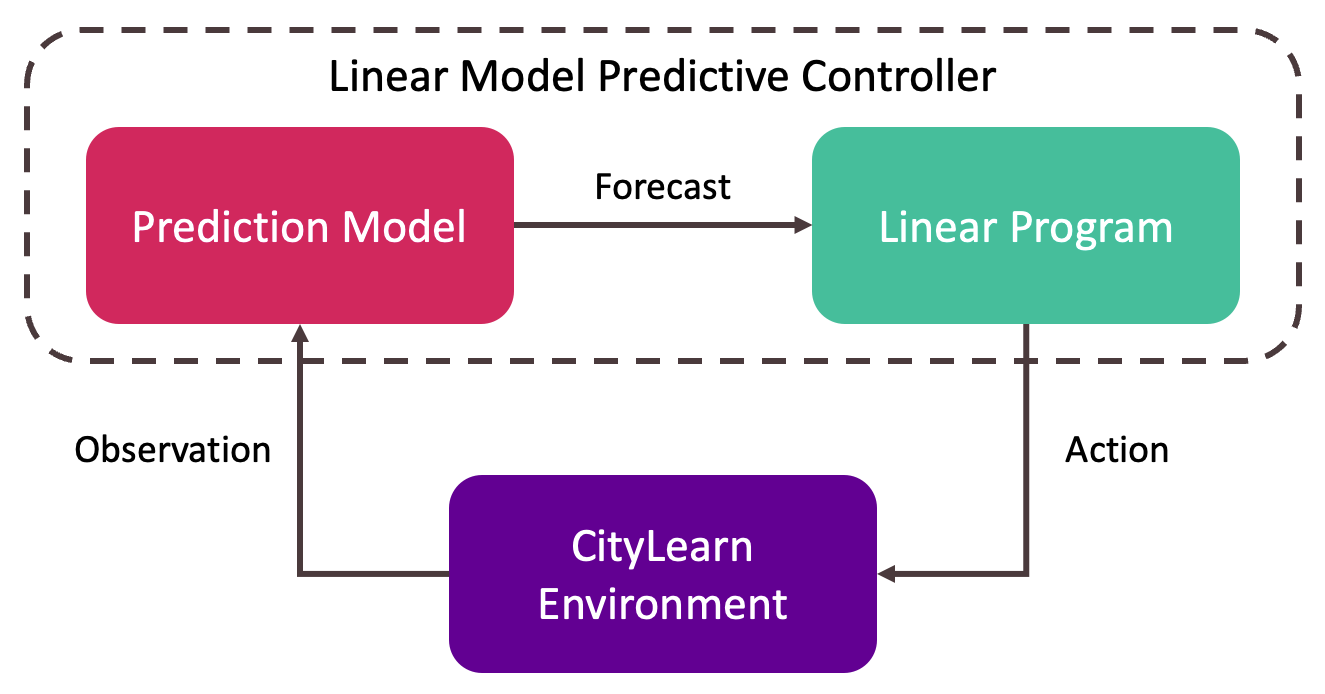
\includegraphics[width=0.66\textwidth]{Task/control-loop.png}
    \caption{Control loop for  test district-level building energy system simulation.}
    \label{fig:forecasting-control-loop}
\end{figure}

\newpage
The Linear Program formulation used in the \glsxtrshort{mpc} scheme is described by Eq. \ref{eq:forecasting-LP-example}, with Table \ref{tab:forecasting-LP-params} providing descriptions of the parameters. At each time step the optimised control actions, ${E_i}^*[\tau{=}0]$, are taken. The optimisation objective is comprised of three weighted components, which correspond to the cost of grid electricity consumed by the buildings (assuming no net electricity metering), the embodied carbon emissions associated with the grid electricity, and the ramping of the overall grid electrical demand which represents the grid impact. The three components are normalised by the values they would have if no battery storage were present in the buildings, denoted by $\widetilde{O}^k$ for component $k$, lower bounded at 1. This clipping is performed to prevent ill-conditioning of the objective when the no-storage objective values are small.

% Note that MPC system model is exact (designed for perfect match between simulator and controller), so only noise is from predictions (isolates impact) - we can get this because we are studying solar-battery systems (no heat), so say this is a reason why we chose a solar-battery system (electrical physics easy).

The CityLearn simulations are configured so that the building energy system has linear dynamics, which is possible as a solar-battery system is studied and only electrical behaviour is considered. As the system parameters are known to the controller, the \glsxtrshort{mpc} has a perfect model of the true system dynamics. This perfect match between the simulator and controller dynamics models means no inaccuracies are introduced in system identification. The optimality guarantees of Linear Programming, and the use of the global operational objective as the \glsxtrshort{mpc} objective, with sufficiently large planning horizon $T$, mean there is negligible distortion of the operational performance from these factors. This allows the effect of operational condition forecast accuracy on \glsxtrshort{mpc} operational performance to be studied in isolation - i.e. to a good approximation, sub-optimality in operational performance in the simulation environment is caused solely by forecasting inaccuracies.\\

\begin{figure}[h]
    \centering
    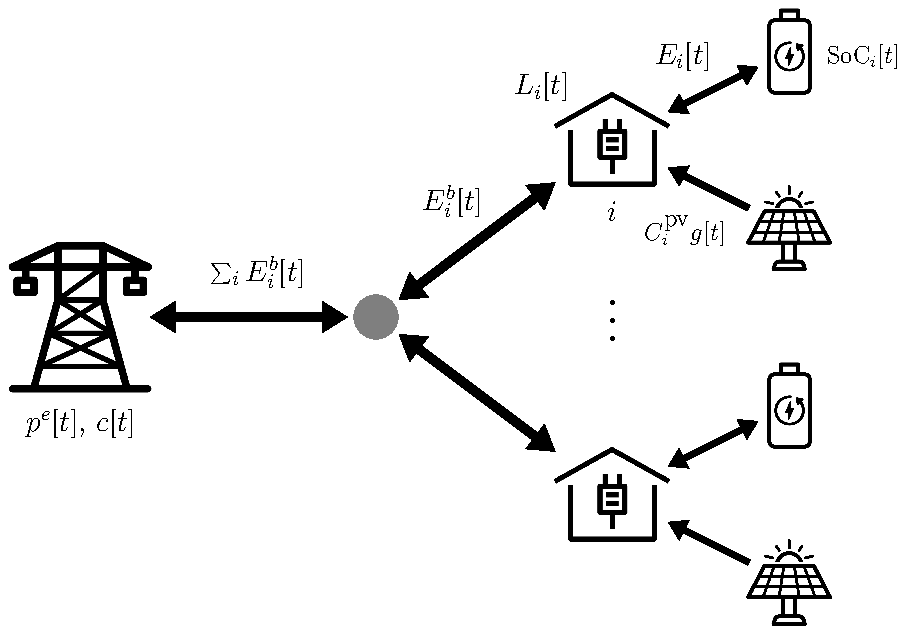
\includegraphics[width=0.7\linewidth]{Task/sys-diagram.pdf}
    \caption{Energy flow schematic for test multi-building energy system. {\small(Icon credits: \href{https://thenounproject.com/symbolon/}{Symbolon})}}
    \label{fig:forecasting-energy-system}
\end{figure}

\newpage
\begin{subequations} \label{eq:forecasting-LP-example}
    \begin{align}
        \addtocounter{equation}{-1}
        \begin{split}
        \text{min} & \qquad \frac{\gamma^p \,\, \mathlarger{\sum}_{\tau} \,\, p^e[t{+}\tau] \, \mathlarger{\sum_i} \left( \max \left[ 0,\, E_i^b[t{+}\tau] \right] \right)}{\raisebox{-1.2ex}{$\max \left[ 1, \widetilde{O}^p \right]$}} \\[1em]
        & \qquad\qquad + \,\, \frac{\gamma^c \,\, \mathlarger{\sum}_{\tau} \,\, c[t{+}\tau] \, \mathlarger{\sum_i} \left( \max \left[ 0,\, E_i^b[t{+}\tau] \right] \right)}{\raisebox{-1.2ex}{$\max \left[ 1, \widetilde{O}^c \right]$}} \\[1em]
        & \qquad\qquad\qquad\qquad + \,\, \frac{\gamma^r \,\, \mathlarger{\sum}_{\tau} \,\, \abs{\bigg( \mathlarger{\sum_i} \, E_i^b[t{+}\tau] \bigg) - \bigg( \mathlarger{\sum_i} \, E_i^b[t{+}\tau{-}1] \bigg)} }{\raisebox{-1.2ex}{$\max \left[ 1, \widetilde{O}^r \right]$}}
        \end{split} \label{eq:forecasting-lp} \\[1ex]
        \text{over} & \qquad E_i[\tau] , \, \textrm{SoC}_i[\tau{+}1] \quad \forall \: i,\, \tau \tag*{} \\
        \text{subject to} & \qquad \textrm{SoC}_i[\tau{+}1] \leq \textrm{SoC}_i[\tau] + \min\left[ E_i[\tau] \sqrt{\eta_i},\, E_i[\tau]/\sqrt{\eta_i} \right] \label{eq:forecasting-dynamics-constraint} \\
        & \qquad -P^{\textrm{max}}_i \Delta t \leq E_i[\tau] \leq P^{\textrm{max}}_i \Delta t \label{eq:forecasting-power-constraint} \\
        & \qquad 0 \leq \textrm{SoC}_i[\tau{+}1] \leq C^s_i \label{eq:forecasting-energy-constraint} \\
        & \qquad \textrm{SoC}_i[\tau{=}0] = \textrm{SoC}_i^t \label{eq:forecasting-initial-conditions} \\
        & \qquad E^b_i[\tau] = L_i[\tau] - C^{\textrm{pv}}_i g[\tau] + E_i[\tau] \label{eq:forecasting-aggregation-constraint} \\
        \text{for all} & \qquad i \in [0,B{-}1], \: \tau \in [0,T{-}1] \tag*{}
        % \text{apply actions} & \qquad E_i[\tau{=}0] \quad \forall \: i \tag*{}
    \end{align}
\end{subequations}

\newpage
\begin{table}[h]
    \centering
    \renewcommand{\arraystretch}{1.25}
    \begin{tabularx}{\linewidth}{ccX} \toprule \toprule
        Parameter & Units & \multicolumn{1}{>{\centering\arraybackslash}c}{Description} \\
        \midrule \midrule
        \multicolumn{3}{>{\centering\arraybackslash}l}{\small\it \quad Decision variables} \\
        $E_i[\tau]$ & kWh & Energy \textit{intake} to battery unit in building $i$ at time $\tau$ in planning horizon \\
        $\textrm{SoC}_i[\tau]$ & kWh & State-of-charge of battery unit in building $i$ at time $\tau$ in planning horizon \\
        \midrule
        \multicolumn{3}{>{\centering\arraybackslash}l}{\small\it \quad Data variables} \\
        $\Delta t$ & hrs & Time step of simulation data \\
        $C^s_i$ & kWh & Energy capacity of battery unit in building $i$ \\
        $C^{\textrm{pv}}_i$ & kWp & Peak power capacity of solar PV unit in building $i$ \\
        $\eta_i$ & -- & Round-trip efficiency of battery unit in building $i$ \\
        $P^{\textrm{max}}_i$ & kW & Power capacity of battery unit in building $i$ \\
        $\textrm{SoC}_i^t$ & kWh &  State-of-charge of battery unit in building $i$ at time $t$ \\
        $L_i[t]$ & kWh & Electrical demand of building $i$ at time $t$ \\
        $g[t]$ & kW/kWp & Normalised generation power from solar PV at time $t$ \\
        $p^e[t]$ & £/kWh & Grid electricity price at time $t$ \\
        $c[t]$ & kgCO$_2$/kWh & Carbon intensity of grid electricity at time $t$ \\
        $\gamma^p$ & -- & Fraction of objective from electricity cost component \\
        $\gamma^c$ & -- & Fraction of objective from CO$_2$ emissions component \\
        $\gamma^r$ & -- & Fraction of objective from grid ramping component \\
        \bottomrule \bottomrule
    \end{tabularx}
    \smallskip
    \caption{Description of Linear Program model parameters.} \label{tab:forecasting-LP-params}
\end{table}


\clearpage
\subsection{Forecasting task \& performance evaluation}

% Explicitly define the prediction task and explain accuracy metrics used to compare forecast qualities and that control performance is also used as it grounds prediction task in context

For the \glsxtrshort{mpc} scheme used, Eq. \ref{eq:forecasting-LP-example}, forecasts of the following operational condition variables over the planning horizon $T$ are required at each time instance, $t$:
\begin{itemize}
    \item electrical demand for each building, $L_i[t]$
    \item normalised solar PV generation power, $g[t]$
    \item price of grid electricity, $p^e[t]$
    \item carbon intensity of grid electricity, $c[t]$
\end{itemize}

This study investigates the impacts of data on the forecasting of these 4 types of operational variables. The accuracies of these forecasts are quantified using two error metrics, the normalised Mean Absolute Error (nMAE), and the normalised Root Mean Squared Error (nRMSE), given by Eqns \ref{eq:forecasting-nMAE} \& \ref{eq:forecasting-nRMSE},

\vspace*{0.5cm}
\begin{minipage}{0.5\linewidth}
\begin{equation} \label{eq:forecasting-nMAE}
    \frac{\frac{1}{N} \mathlarger{\sum_{t=0}^{N-1}} \, \frac{1}{T} \sum_{\tau=1}^{T} \abs{f^v_{t,\tau} - v_{t+\tau} } }{\frac{1}{N} \sum_{t=0}^{N-1} v_t}
\end{equation}
\end{minipage}%
\begin{minipage}{0.5\linewidth}
\begin{equation} \label{eq:forecasting-nRMSE}
    \frac{\frac{1}{N} \mathlarger{\sum_{t=0}^{N-1}} \sqrt{ \frac{1}{T} \sum_{\tau=1}^{T} \left(f^v_{t,\tau} - v_{t+\tau} \right)^2 } }{\frac{1}{N} \sum_{t=0}^{N-1} v_t}
\end{equation}
\end{minipage}
\vspace*{0.5cm}

where $f^v_{t,\tau}$ is the forecast of variable $v$ at time $t$ for time instance $\tau$ in the planning horizon, and $v_{t+\tau}$ is the true value of the target variable at time instance $t+\tau$. These error metrics are the means of the standard MAE and RMSE errors over all forecasting horizons considered in the simulation, normalised by the mean level of the target variables to allow comparability between forecast accuracies.

The operational performance achieved by the \glsxtrshort{mpc} scheme using a given set of prediction models is quantified by evaluating the objective specified in Eq. \ref{eq:forecasting-LP-example} with the simulated behaviour of the building energy system resulting from the use of the controller.

All experiments conducted in this study test the same multi-building energy system, with distributed energy assets as specified in Appendix \ref{app:forecasting-system-spec}, and use a planning horizon of $T=48$hrs, justification of this value is provided in Appendix \ref{app:forecasting-tau}, along with objective component weights, $(\gamma^p,\gamma^c,\gamma^r) = (0.45,0.45,0.1)$, in both the \glsxtrshort{mpc} scheme and for operational performance evaluation.


\newpage
\subsection{Building electricity usage data}

Historic building electricity metering data from the Cambridge University Estates dataset \citep{langtry2024CambridgeUniversityEstates}, described in Appendix \ref{app:data}, is used to provide a case study for the multi-building energy system. A 10 year period from 2010 to 2019 is chosen for the case study, so that data durations up to a maximum practical length can be tested. 15 buildings\footnote{The number of buildings that can be used in the study is limited by the computational cost of the forecasting methods and the system simulations.} with complete data availability for electrical load over this period are selected\footnote{Version 1 building numbers: 0, 3, 9, 11, 12, 15, 16, 25, 26, 32, 38, 44, 45, 48, 49} for use in the experiments, such that they cover a wide range of building scales and provide a good mix of similarity and dissimilarity with respect to their electricity loads.

Alongside the building electrical load data, which is assumed not to contain any significant contributions from space heating or cooling, the following other data variables are retrieved from the dataset: weather data for Cambridge (including outdoor temperature, relative humidity, and direct \& diffuse solar irradiance), local solar generation power, grid electricity price \& carbon intensity data, and temporal information (including hour, day, month indices, and daylight savings status).

The 10 years of data is initially split into training, validation, and test datasets covering the following periods: train (2010 to 2015), validate (2016 to 2017), test (2018 to 2019). For all experiments the test data is kept the same, however the periods of data used to train the prediction models are altered in Section \ref{sec:forecasting-data-efficiency}.

\subsection{Brief description of the prediction models}

% Briefly outline models studied. We pit simple models against SOTA. Offload technical details to \ref{app:forecasting-models}.

Data and computational requirements, which vary across predictions models, are important considerations for the deployment of \glsxtrshort{mpc} based controllers in practical building energy systems. This work investigates the performance of 6 machine learning based prediction models which span a range of model characteristics; 3 simple neural models, and 3 high-complexity, state-of-the-art models. A brief description of each model architecture follows. Technical specifications of the model implementations used are provided in Appendix \ref{app:forecasting-models}.

\subsubsection{Simple neural models}

Recent literature, \citep{zeng2023AreTransformersEffective}, has shown that simple neural models using Direct Multi-Step forecasting (DMS), where all predictions over the forecast window are generated concurrently, can outperform complex, transformer-based models using traditional, Iterated Multi-Step forecasting (IMS), in which a single-step forecaster is applied iteratively to generate a multi-step forecast. For all three simple neural architectures investigated, DMS forecasting is used.

\paragraph{Linear neural network (Linear)}

A Multi-Layer Perceptron (MLP) model that maps the inputs directly to the output without an activation function (non-linearity).

\paragraph{Residual multi-layer perceptron (ResMLP)}

A Residual MLPSkip model (MLP model with skip-connections), comprised of a single hidden layer with 128 neurons.

\paragraph{Convolutional neural network (Conv)}

A Convolutional Neural Network (CNN) model that contains convolution layers followed by a linear layer. The architecture used comprises two layers with kernel sizes of 6 and 12, with five and one channels, respectively.

\subsubsection{State-of-the-art machine learning models}

\paragraph{Temporal Fusion Transformer}

The Temporal Fusion Transformer (TFT) model \citep{lim2021TemporalFusionTransformers}, developed by Google, is an attention-based architecture that enables the fusion of data from multiple input sources to inform predictions. The neural structure contains features which allow for the learning of multiple underlying relationships across temporal scales, and the attention mechanism allows for interpretation of the model predictions, i.e. which data the model is exploiting to produce its forecasts. The model uses categorical covariates of date-time information, as well as temperature information for predicting building loads.

\paragraph{Neural Hierarchical Interpolation for Time Series Forecasting}

Neural Hierarchical Interpolation for Time Series Forecasting (NHiTS) \citep{challu2023NHITSNeuralHierarchical} is an MLP model which learns a set of basis functions at different frequencies that describe the underlying patterns in the training data, and produces forecasts by using hierarchical interpolation to combine predictions from the basis functions in a computationally efficient manner. It uses categorical covariates of date-time information.

\paragraph{DeepAR}

DeepAR is a Recurrent Neural Network (RNN) based model developed by Amazon \citep{salinas2020DeepARProbabilisticForecasting}, which has been widely applied in a range of research areas. It is a probabilistic forecasting model, but for this study only the mean prediction is used. The model uses categorical covariates of date-time information.\\


\newpage
%********************************** Results section **************************************
\section{Results \& Discussion}

% Go through the results we have and discuss in situ.

%% NOTE: keep terminonolgy consistent - accuracy for forecasts, performance for control !!!

\subsection{Baseline prediction accuracy comparison} \label{sec:forecasting-baseline-comparison}

The prediction accuracy of each forecasting model trained using 8 years of training data, the maximum available, was evaluated to provide a baseline for the model architectures in a setting without data limitations. For brevity, forecast accuracy results are discussed for the nRMSE metric only, however equivalent results were found with the nMAE metric. Figures \ref{fig:forecasting-baseline-load-comparison} \& \ref{fig:forecasting-baseline-PCS-comparison} show that the simple Linear model achieves similar or better prediction accuracy (lower nRMSE values) compared to the complex, state-of-the-art models across all prediction variables. The Conv and ResMLP models provide similar accuracy when predicting building electrical loads, however both have significantly worse accuracy for the electricity price and carbon intensity prediction variables. Complex models achieve slightly better accuracy for electricity price and solar generation predictions, at most 8.5\% and 4.2\% lower nRMSE than the Linear model, achieved by NHiTS and TFT respectively. However, for some buildings the complex models exhibit very poor forecast accuracy for load predictions. These instances of poor accuracy are found to correlate with a measure of the similarity between the train and test datasets for building load, called the `Wasserstein similarity metric', which is described in Appendix \ref{app:forecasting-similarity-metric} and is used for the study of model reuse in the following section. Fig. \ref{fig:forecasting-baseline-load-similarity-correlation} plots the relationship between prediction accuracy and data similarity for each model, and shows that complex models provide poor prediction accuracy when the training and test data are significantly different. Hence, simple neural models provide better prediction generalisation under changes in building load dynamics between the training and test data, which is highly advantageous for application to practical systems, as occupant driven load dynamics may change after system installation, e.g. due to a change of building use.

\begin{figure}[ph!]
\centering
\subfloat[Comparison of baseline load prediction accuracy of forecasting models.]{
    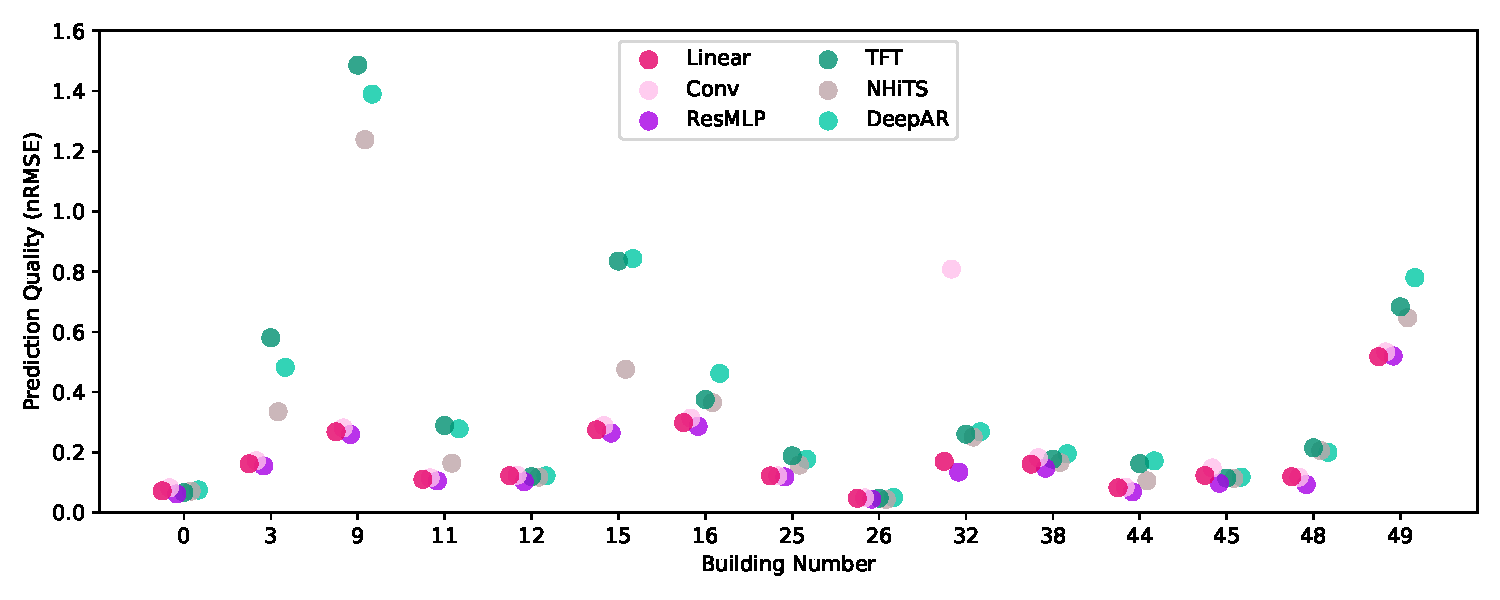
\includegraphics[width=0.9\linewidth]{Comparison/baseline_comparison_load_nRMSE.pdf}
    \label{fig:forecasting-baseline-load-comparison}
}
\bigskip

\subfloat[Correlation between model prediction accuracy and train-test data\\similarity metric value (lower Wasserstein metric means more similar data).]{
    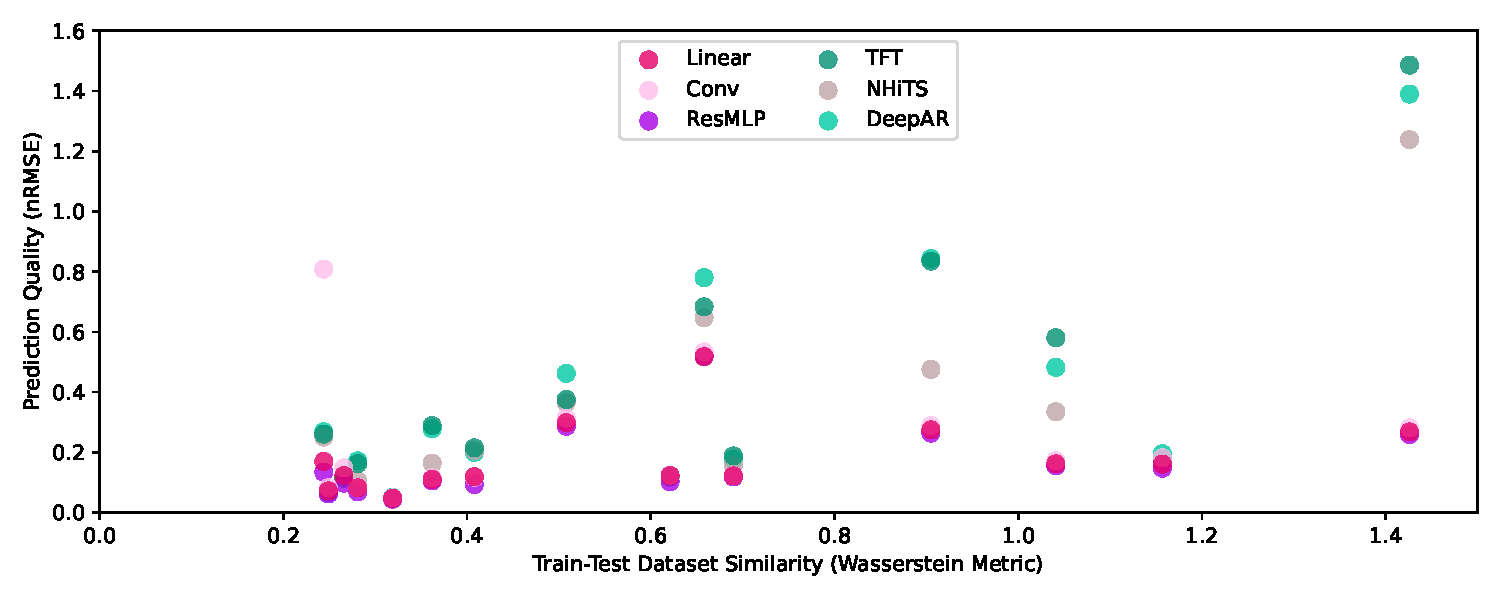
\includegraphics[width=0.9\linewidth]{Comparison/baseline_comparison_similarity_corr_nRMSE.pdf}
    \label{fig:forecasting-baseline-load-similarity-correlation}
}
\bigskip

\hspace*{\fill}
\subfloat[Pricing, carbon, solar prediction comparison.]{
    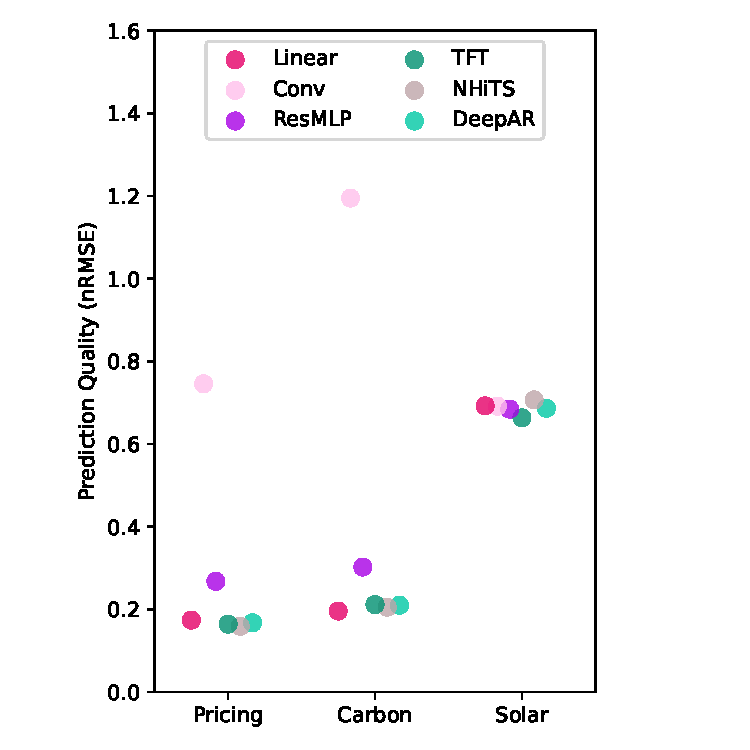
\includegraphics[height=6cm]{Comparison/baseline_comparison_PCS_nRMSE.pdf}
    \label{fig:forecasting-baseline-PCS-comparison}
}%
\hspace*{\fill}
\subfloat[Comparison of \glsxtrshort{mpc} operational performance using baseline forecasting models.]{
    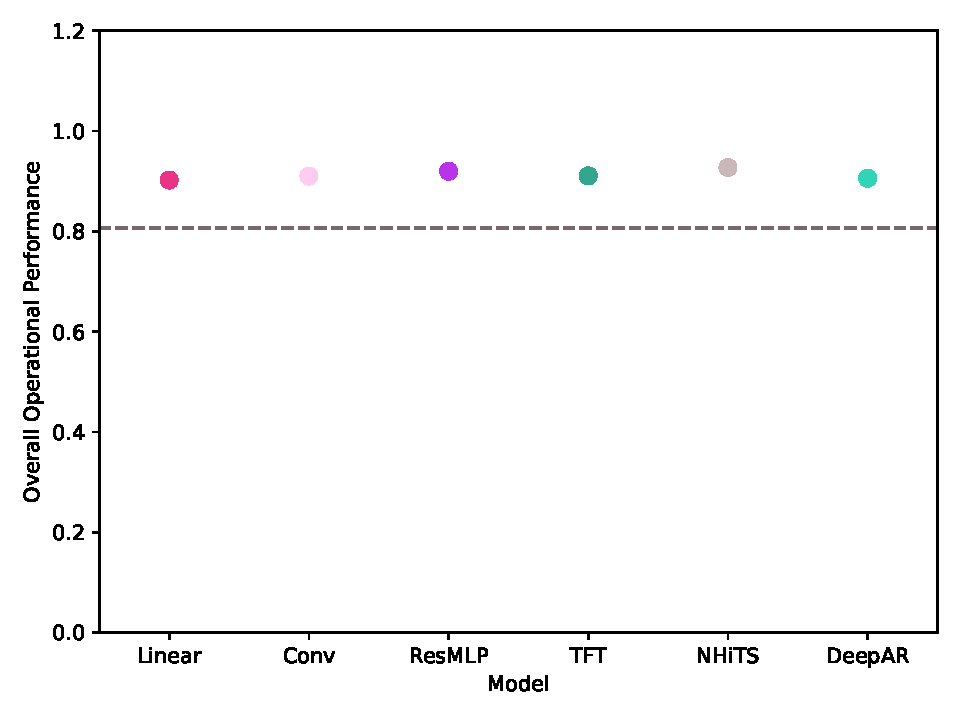
\includegraphics[height=6cm]{Comparison/baseline_comparison_evaluate.pdf}
    \label{fig:forecasting-baseline-evaluate-comparison}
}\hspace*{\fill}

\smallskip
\caption{Comparison of baseline prediction accuracy and operational performance of forecasting models.}
\label{fig:forecasting-baseline-comparison}
\end{figure}

These results indicate that simple neural models have sufficient expressivity to well capture the underlying trends in building energy usage, but learn sufficiently simple relationships about the data as to avoid the problem of over-fitting experienced by the complex models, leading to better generalisation in time. This suggests that the majority of the trends in the load data are present within the 1 week input window used by the simple models, which agrees with the strong daily and weekly trends of typical building energy usage, caused by building occupancy patterns. It is likely that annual trends are well captured by the mean value over the input window, as these trends are slow relative to the prediction length. Additionally, the predictions required by \glsxtrshort{mpc} are relatively short in length, 48 hours in this case, whereas the complex models are found to provide more stable predictions and greater overall accuracy for longer duration forecasts \citep{challu2023NHITSNeuralHierarchical,zhang2022TemporalFusionTransformer}.

Overall, simple neural models are able to provide analogous prediction accuracy to complex models across all prediction variables, and do so with substantially lower computational requirements. Table \ref{tab:forecasting-comp-times} provides the training time and inference time (time to generate forecasts) of the baseline models, and shows that simple models require roughly 500x less computation for inference. Hence, in practical systems the use of simple models would enable shorter prediction intervals, leading to higher frequency control, and allow for the use of lower cost compute hardware. Further, due to their high computational cost, the complex models were only able to use a 72 hour input window \citep{lopezsantos2022ApplicationTemporalFusion}. As a result, they have less information available to inform their predictions, likely limiting the accuracy they could achieve. Therefore, the computational efficiency of simple neural models enabling the use of longer input windows provides an additional advantage.\\

\begin{table}[h]
    \centering
    \renewcommand{\arraystretch}{1}
    \begin{tabularx}{\linewidth}{c|*{6}{X}} \toprule \toprule
        Model & Linear & Conv & ResMLP & TFT & NHiTS & DeepAR \\ \midrule
        Training time (hrs) & 12.3 & 26.8 & 13.4 & 8.9 & 15.2 & 9.3 \\
        Prediction inference time (s) & 29 & 73 & 146 & 15,222 & 15,289 & 74,991 \\ \bottomrule\bottomrule
    \end{tabularx}
    \smallskip
    \caption{Computation times for baseline models, trained on 8 years of data, and predicting for simulations of 2 years duration.}
    \label{tab:forecasting-comp-times}
\end{table}

The similar prediction accuracies of the tested models are found to lead to similar operational performance when used in the \glsxtrshort{mpc} scheme, see Fig. \ref{fig:forecasting-baseline-evaluate-comparison}, where the dashed line indicates the bound on operational performance achieved by an \glsxtrshort{mpc} scheme with perfect forecasts. The use of the \glsxtrshort{mpc} controllers with the specified battery systems leads to an average 8.7\% improvement in operational performance for the multi-building energy system, with a range of 7.3\% to 9.8\%.\\


\subsection{Model generalisation} \label{sec:forecasting-generalisation}

% Can data be reused? (Is it worth reusing?)
% Train on one building, test on another, how good is it?

When a solar-battery system using \glsxtrshort{mpc} is installed, high-resolution historic load metering data (e.g. from smart meters) may not be available for the building. In this case, the project must either be delayed to allow time for data collection, incurring a significant cost, or a prediction model trained on load data from another building must be used, potentially incurring an operational performance penalty due to worse prediction accuracy. Model reuse greatly reduces data collection requirements and the associated costs, however its appropriacy depends on the ability of load prediction models to generalise between buildings, and the trade-off between data cost savings and increased operational cost due to lower forecast accuracies.

The generalisation of prediction models between buildings is tested by using the baseline models trained on data from each of the 15 buildings to forecast electrical load for every other building. Fig. \ref{fig:forecasting-generalisation-violin} shows the distribution of relative forecast accuracies achieved by each model over all buildings (DeepAR is excluded due to excessive computational costs), where the y-axis plots the nRMSE forecast accuracy of the tested model (potentially trained on a different building) normalised by the forecast accuracy achieved by the model trained on data from the target building.\\

\begin{figure}[h]
    \centering
    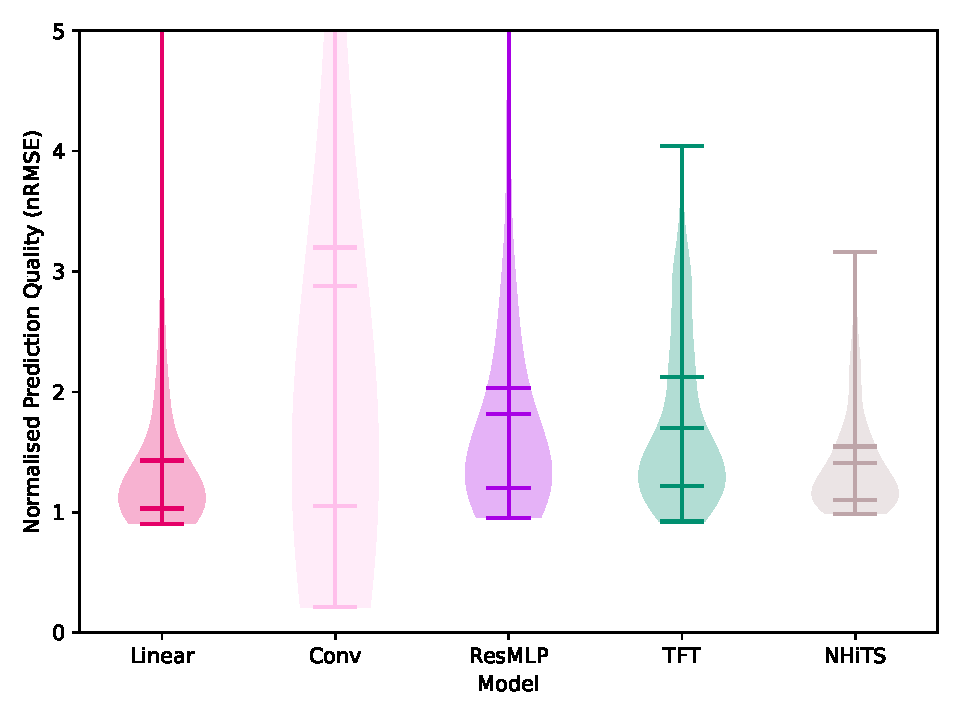
\includegraphics[width=0.7\linewidth]{Generalisation/generalisation_violin.pdf}
    \vspace*{-0.5cm}
    \caption{Comparison of forecasting model generalisation. Violin plot with quartiles indicated by horizontal lines.}
    \label{fig:forecasting-generalisation-violin}
\end{figure}
\bigskip

The Linear model provides similar generalisation performance to NHiTS, and is substantially better than all other models. It is proposed that the Linear model, being mechanistically equivalent to linear regression, achieves good generalisation as it learns relatively simple relationships about the load data, which are consistent between buildings. Whereas NHiTS achieves good generalisation due to its behaviour of generating smooth forecasts \citep{challu2023NHITSNeuralHierarchical}, making it less susceptible to producing erratic and inaccurate predictions with unseen input data. As before, TFT suffers from over-fitting, leading to relatively poor generalisation. Whilst the Conv model was able to provide good generalisation in time where the dataset similarity was close, indicated by small Wasserstein metric values in Fig. \ref{fig:forecasting-baseline-load-similarity-correlation}, between buildings the load data is much less similar, and the relationships learned by the Conv model are no longer valid, leading to poor prediction accuracy. It is suggested this is due to the features learned by the pooling process no longer being pertinent for the new building.\\

If a pre-trained Linear model is selected for reuse at random, the average prediction accuracy is substantially worse than a model trained on data collected from the target building (45\% higher nRMSE, corresponding to the mean of the violin plot). However, in a real scenario where an ensemble of pre-trained models is available, the smart energy storage system designer could reuse a model from a building that is expected to be similar to the target building (e.g. by size, usage type, envelope characteristics, load dynamics, etc.), to maximise the likelihood of good generalisation. A load profile similarity metric is additionally proposed as a way off assessing the similarity of building load dynamics for the purposes of model reuse. This similarity metric is based on the similarity of the distributions of underlying mode shapes within each load profile, and is referred to as the `Wasserstein similarity metric' as it uses the Wasserstein distance between mode shape coefficient distributions. Appendix \ref{app:forecasting-similarity-metric} describes the calculation of similarity metric values. The correlation between generalisation of the Linear model and the Wasserstein similarity metric values between the training datasets of the reused model building and target building is shown in Fig. \ref{fig:forecasting-generalisation-linear-Wass-corr}. The cluster of points in the bottom left indicates that buildings with similar load profiles (low Wasserstein metric values) can provide models that achieve good generalisation. When selecting models for reuse by minimising the Wasserstein metric, the average relative prediction accuracy improves to an 11\% increase in nRMSE, with a range of -7.9\% to +52.6\%, showing that some reused models outperform those trained on the true building training dataset.

\begin{figure}[h]
    \centering
    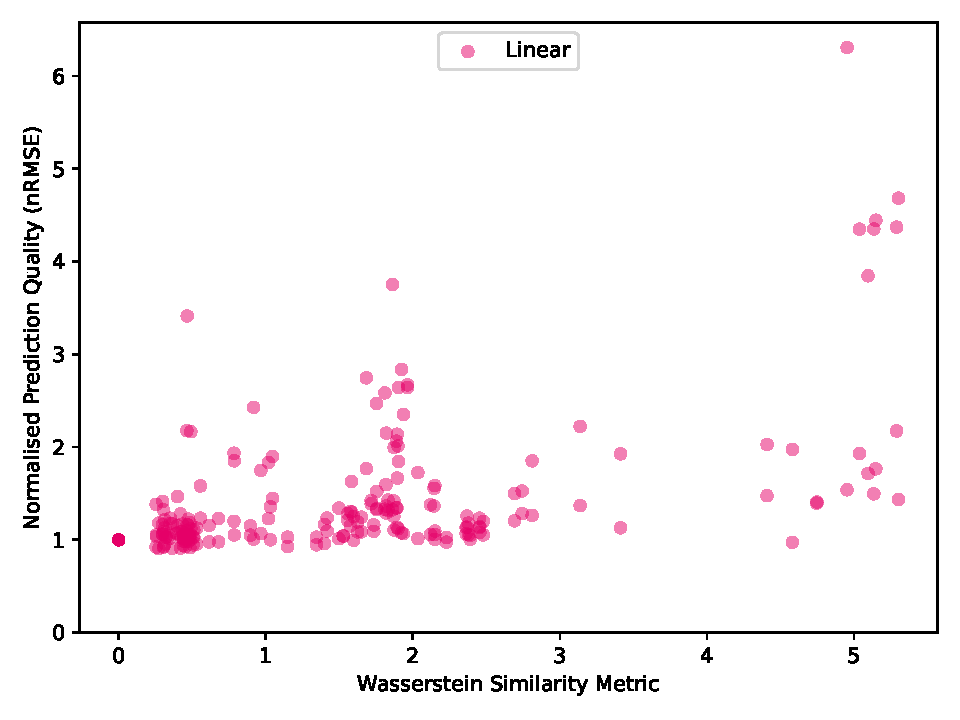
\includegraphics[width=0.7\linewidth]{Generalisation/generalisation_linear_similarity_corr.pdf}
    \caption{Correlation between Linear model generalisation and training dataset similarity metric values.}
    \label{fig:forecasting-generalisation-linear-Wass-corr}
\end{figure}

These results show that when developing a load forecasting model for a new building system where little or no data is available, the reuse of forecasting models trained on existing buildings provides a promising\footnote{Further work is required to determine the feasibility of identifying similar buildings from the model ensemble in practice. Whilst a small sample of load data from the target building could be used to approximate the Wasserstein similarity metric, the quality of this approximation must be weighed against the forecast accuracy that could be achieved by a model trained using that data. Though, additional information on the building, such as usage type, could be used to guide model selection for reuse.} alternative to the collection of data and training of a building specific model, and the associated costs. However, reusing prediction models increases uncertainty in the operational performance the \glsxtrshort{mpc} system will achieve, as models trained on load data from buildings similar to the target building do not always provide good prediction accuracy, as shown by the wide range of reused model accuracies.


\newpage
\subsection{Data efficiency} \label{sec:forecasting-data-efficiency}

% Can the data efficiency of models be improved? What are the trade-offs between data usage and prediction quality?

Data required for developing forecasting models incurs cost from both its acquisition and the computation required to exploit it. However, using longer durations of training data or additional data variables can increase forecast accuracy, resulting in lower operational cost of the energy system. Therefore, any measures to reduce the quantity of data used must be traded-off against the corresponding decrease in prediction accuracy. This section explores a series of aspects of data efficiency and their effect on forecast accuracy. Subsequently, Section \ref{sec:forecasting-control-sensitivity} investigates the impact of forecast accuracy on operational performance of the \glsxtrshort{mpc}.

Testing data efficiency requires several versions of a prediction model to be trained. Due to computational limitations, for some data efficiency tests only the Linear prediction model is studied, as the complex models are too computationally expensive, and results from previous sections show the Linear model is the best performing simple model.

\subsubsection{Volume of training data} \label{sec:forecasting-data-efficiency-training-data}

% Use less data, what happens to prediction quality?

Using greater volumes of training data, longer durations of historic measurements of buildings, can improve model prediction accuracy by avoiding over-fitting, improving temporal generalisability, but comes at a roughly linear cost. The trade-off between the length of training data used, the combined duration of the train and validate datasets, and forecast accuracy is investigated by training prediction models on subsets of the building energy dataset of varying durations from 8 years, the maximum duration available, to 3 months (one season), the shortest duration tested in \citep{choi2023PerformanceEvaluationDeep}. For the complex models, at least 2 years of training data was required due to the use of temporal covariates. Fig. \ref{fig:forecasting-data-eff-n-training-years} plots the proportional improvement in prediction accuracy of each model (negative improvement shows worsening model accuracy) compared to baseline when training using different data volumes. Across a broad range of model architectures, reducing training data length down to 2 years has a limited impact on prediction accuracy, in some cases improving prediction accuracy. Trends differ between prediction variables, however for the Linear model, in the majority of cases there is a small prediction accuracy penalty between 8 and 1 years of training data, and then a rapid worsening of forecasting accuracy below 6 months.
This indicates that when making data collection decisions to support prediction model development for building electrical energy systems, at most 2 years of measurement data should be gathered. However, at least two seasons of data (6 months) are required to prevent model over-fitting and learn trends which generalise across seasons.

\begin{figure}
    \centering
    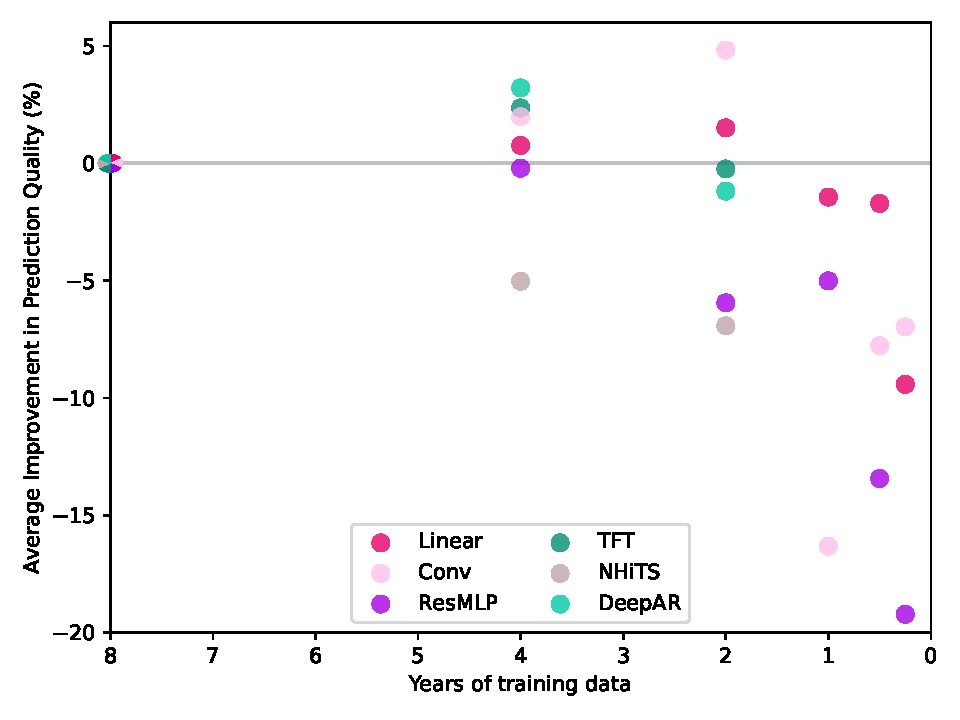
\includegraphics[width=0.7\linewidth]{Data_Efficiency/prediction_vs_n_training_years.pdf}
    \caption{Average improvement in prediction accuracy over all prediction variables with years of data used for training.}
    \label{fig:forecasting-data-eff-n-training-years}
\end{figure}


\paragraph{Screening training data using change-points} \label{sec:forecasting-data-efficiency-change-point}

% Use less data, excluding training data in an intelligent way, what happens to prediction quality?
% Use identified change-points from analysis in Section \ref{sec:change-points} to see if removal of non-representative training data can improve model performance and data efficiency - use multiple change-points only.
% Do our results correspond with those from \citep{choi2023PerformanceEvaluationDeep} that not all additional training data is useful, only the similar sections? Acknowledge data similarity study in Wonjun's paper in discussion - yes, but trade-off between use of non-representative data and having enough data to avoid over-fitting. Unlike Wonjun's results, we are testing on 2years of data (he only tests on 0.1yrs), so I think we need at least a full years of data to capture all of the seasonality in the model.
% Note this is a very simple screening method, and assessing similarity of chunks to validation data would like provide a better method (though this assumes validation data is most representative of test data...), we could use the Wasserstein metric for this.

Once building data has been gathered, there remains a question as to whether all of the available data should be used for training, or whether some data should be excluded to improve model prediction. For instance, if data that is non-representative of the present building load dynamics can be excluded, prediction accuracy can be improved alongside data efficiency.
Change-point analysis can be used to screen training data for this purpose, by detecting changes in building load dynamics and excluding data preceding the change from training. A change-point analysis using the BEAST algorithm \citep{zhao2019DetectingChangepointTrend} was performed on the building load dataset, described in Appendix \ref{app:forecasting-change-points}. Points where changes in load trend were detected were used to screen the training data for 7 selected buildings. In order to allow a better analysis of the detected change-points, the training dataset was increased to 7 years (2010-2016), leaving 1 year of validation data (2017). Linear prediction models were trained using sections of the training data starting at each detected change-point and running to the end of 2016.

\begin{figure}
    \centering
    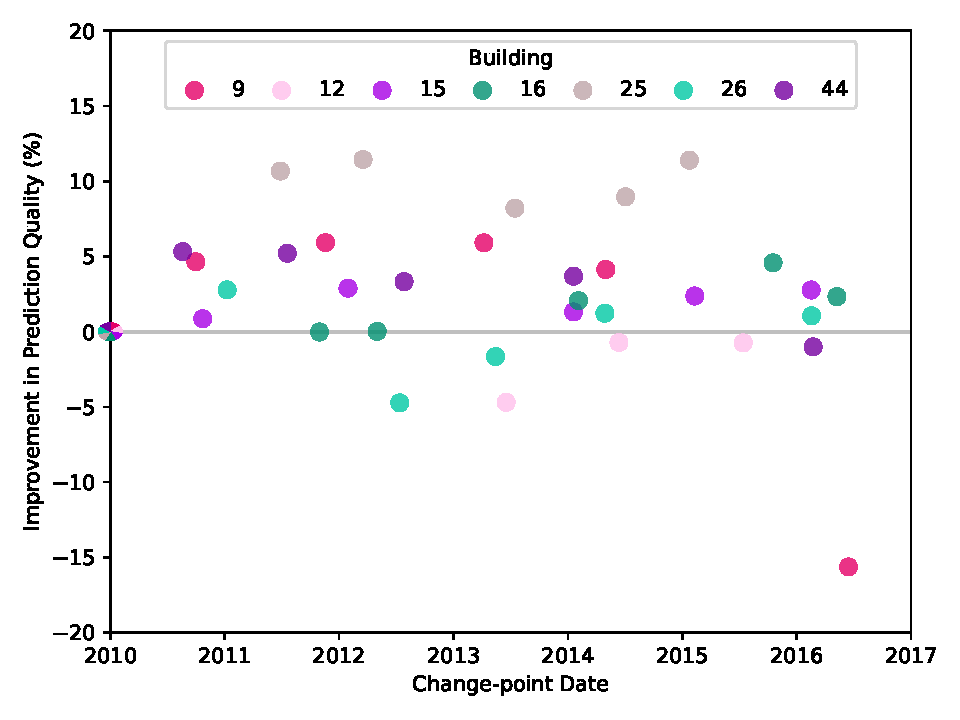
\includegraphics[width=0.7\linewidth]{Data_Efficiency/chagepoint_prediction_performance.pdf}
    \caption{Improvement in prediction accuracy of models trained using data from change-points onward.}
    \label{fig:forecasting-data-eff-changepoints}
\end{figure}

Fig. \ref{fig:forecasting-data-eff-changepoints} shows the relative improvements in prediction accuracy of models trained on data screened using change-points, compared to the case where the full 7 years of available data is used, where the x-axis position indicates the timing of the change-point. For most buildings, screening the training data using change-points improves prediction accuracy, indicating that non-representative data is being removed from the training dataset. This suggests that ex-post training data screening can be used to improve model accuracy whilst reducing the quantity of training data used, and so computational cost. These results correspond with the findings of \citep{choi2023PerformanceEvaluationDeep}, which shows that additional training data only improves prediction accuracy if it is sufficiently similar to the test data, and can reduce accuracy when insufficiently similar. However, the results of this study demonstrate an additional consideration, which is that prediction accuracy worsens substantially when insufficient training data volume is used. This suggests a trade-off between having enough data to avoid over-fitting, and removing non-representative data which causes over-generalisation of the model. Figures \ref{fig:forecasting-data-eff-n-training-years} \& \ref{fig:forecasting-data-eff-changepoints} indicate that at least 1 year of training data is required to achieve good prediction accuracy, after which only sufficiently similar data should be included in the training dataset. The reason for the difference in results compared to \citep{choi2023PerformanceEvaluationDeep} is likely due to this study testing model prediction accuracy on 2 years of data, compared to 0.1 years in \citep{choi2023PerformanceEvaluationDeep}. As a result, models in this study must capture the seasonality of building load dynamics, hence requiring at least 1 year of training data to achieve good prediction accuracy.

The data screening method considered in this study is relatively simple, using change-points to exclude data by classifying it as `non-representative' of current behaviour. More advance techniques could be created by quantifying the similarity between the sections of data identified using the change-points and the validation data, e.g. using the Wasserstein similarity metric, and selecting sections of data to use in the training dataset using both the probability of a true change having occurred and the data similarity metrics.

Change-point analysis can also be used online to detect real time changes in building load dynamics and provide indication of when the prediction models should be updated (i.e. retrained using recent data), due to the training data of the current model no longer being representative of the building behaviour, causing reduced prediction accuracy. This is particularly pertinent in the context of climate change, which is expected to significantly impact the energy usage behaviour of buildings, for instance reducing peak heating loads due to higher winter temperatures, and increasing summer electrical loads to provide cooling during prolonged heat waves.

\subsubsection{Data features} \label{sec:forecasting-data-efficiency-data-features}

% Use less data by not measuring some stuff, what happens to prediction quality?

The variables that can be monitored in building energy systems are often well correlated, for example ambient temperature and electrical load. As a result, covariates can be used by prediction models to attempt to identify underlying links between the variables and improve forecast accuracy. However, the use of additional data variables (features) incurs a cost from both the collection and exploitation of the extra data, for instance the purchase of proprietary weather forecasts. The impact of feature selection on forecast accuracy is investigated by comparing the prediction accuracy of models trained using varying numbers of data features. The Pearson correlation coefficient between the 11 data features available in the building energy dataset are shown for the case of Building 0 in Fig. \ref{fig:forecasting-data-eff-variable-correlations}. Linear prediction models were trained using the $n$ most correlated variables/features for each of the electrical load, solar generation, electricity price, and carbon intensity target variables. Feature selection was performed separately for each case by ranking Pearson correlation coefficients between the target variable and all other available covariates. Fig. \ref{fig:forecasting-data-eff-n-variables} shows the impact of the number of data features used by the models on forecast accuracy. For most prediction variables, the inclusion of additional data features worsens forecast accuracy. Several factors could contribute to this behaviour:
\begin{itemize}
    %\setlength\itemsep{0ex}
    \item Over-fitting \citep{hawkins2004ProblemOverfitting} : The incorporation of an excessive number of features may lead the model to over-fit the training data, worsening its predictions for unseen data.
    \item Multi-collinearity \citep{farrar1967MulticollinearityRegressionAnalysis} : The presence of highly correlated features can destabilize the model, resulting in worse prediction accuracy.
    \item Curse of Dimensionality \citep{verleysen2005CurseDimensionalityData} : An increase in the number of features increases the dimensionality of the data, which can lead to data sparsity and degradation of prediction accuracy.
\end{itemize}

\begin{figure}
    \centering
    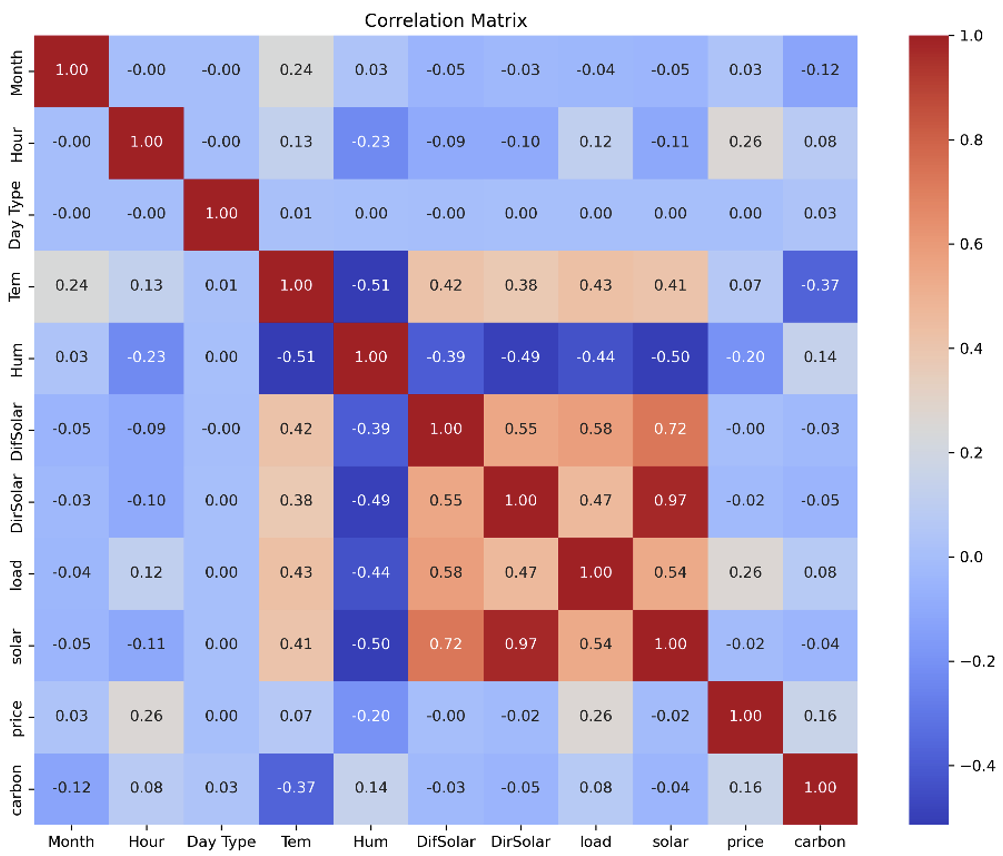
\includegraphics[width=0.5\linewidth]{Data_Efficiency/variable_correleations.png}
    \caption{Pearson correlation between data variables for Building 0.}
    \label{fig:forecasting-data-eff-variable-correlations}
\end{figure}

\begin{figure}[h]
    \centering
    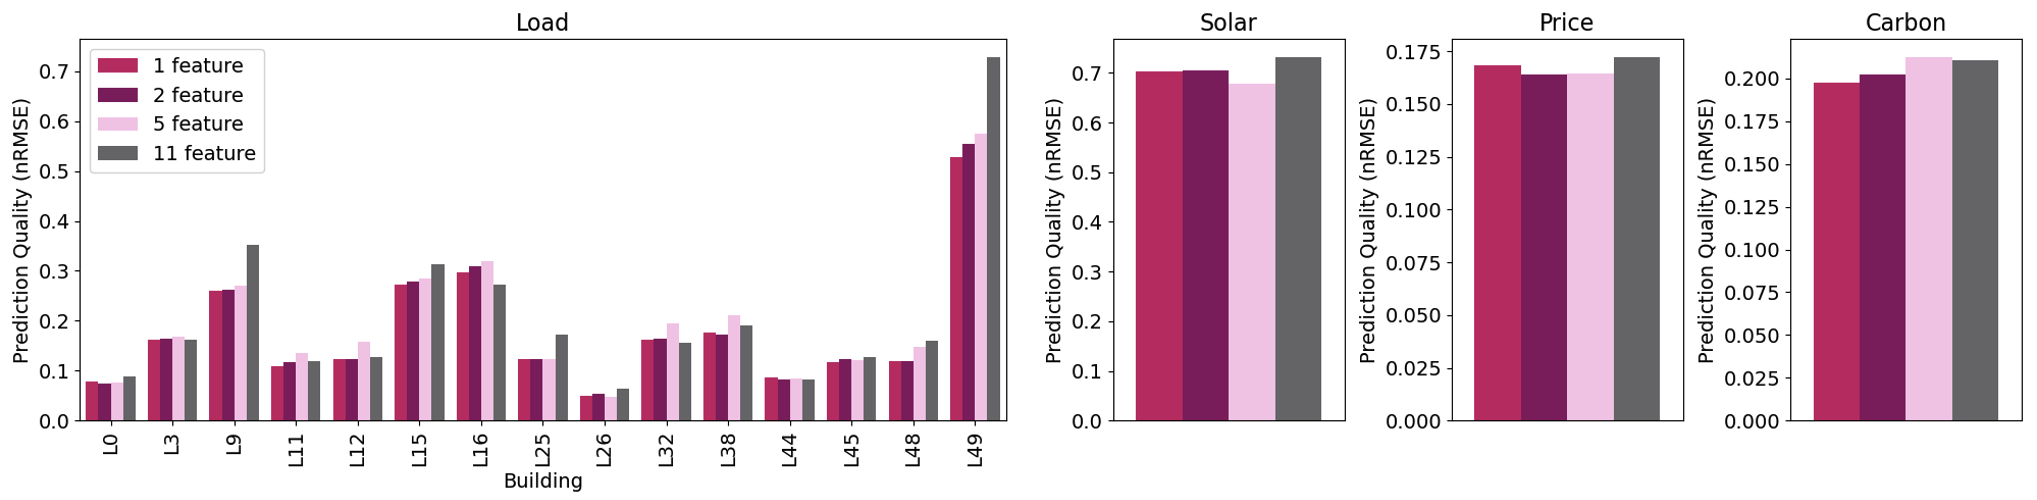
\includegraphics[width=\linewidth]{Data_Efficiency/prediction_vs_n_variables.png}
    \caption{Variation of prediction accuracy with no. of data features included in Linear model.}
    \label{fig:forecasting-data-eff-n-variables}
\end{figure}

These results show that testing should be performed before decisions are made regarding the collection of covariate data to ensure that, for the type of system in question, its use will firstly improve prediction accuracy, and secondly that said accuracy improvements warrant the cost of the data. This study considers a simple, correlation based feature selection method, however more advanced, optimization based techniques \citep{gonzalez-vidal2019MethodologyEnergyMultivariate,kim2020ElectricityLoadForecasting} could be used to determine the set of available features which provides the optimal trade-off between data cost and model prediction accuracy.

\subsubsection{Online training} \label{sec:forecasting-online-training}

% Use all of the data you have available from realtime measurements, how can prediction quality be improved? And is it worth the extra hardware and complexity of the deployed system?

During building operation monitoring systems continuously collect operational data. The characteristics of building behaviour can change during operation due to external factors such as weather \& climate, occupancy, and equipment degradation \& maintenance. Continuous online training updates the predictive models using the collected monitoring data, improving the model's ability to adapt to dynamic changes in building behaviour. A version of the Linear prediction model with online training is implemented to investigate the impact of online training frequency on model accuracy. The model is updated online by tuning the model parameters (retraining) using a sliding window of training data with length equal to the update frequency.
The prediction accuracy of models updated at different frequencies is plotted in Fig. \ref{fig:forecasting-data-eff-update-freq}. Higher update frequencies led to increased prediction accuracy across all prediction variables. For example, prediction accuracy for grid electricity price improved by 15.7\%, 14.0\%, 12.1\%, and 8.1\% when updated monthly, quarterly, semi-annually, and annually, respectively, compared to the baseline model which is not trained online. Online training allows the prediction model to adapt to changes in the underlying trends which occur over time, as it can learn the trends in recent data. This improves prediction accuracy as the model does not need to generalise in time, as it is trained (updated) on data that is representative of the current prediction horizon.
Therefore, it is expected that the additional computational hardware and system complexity required for online trained prediction models will be worthwhile in practical systems.

\begin{figure}[h]
    \centering
    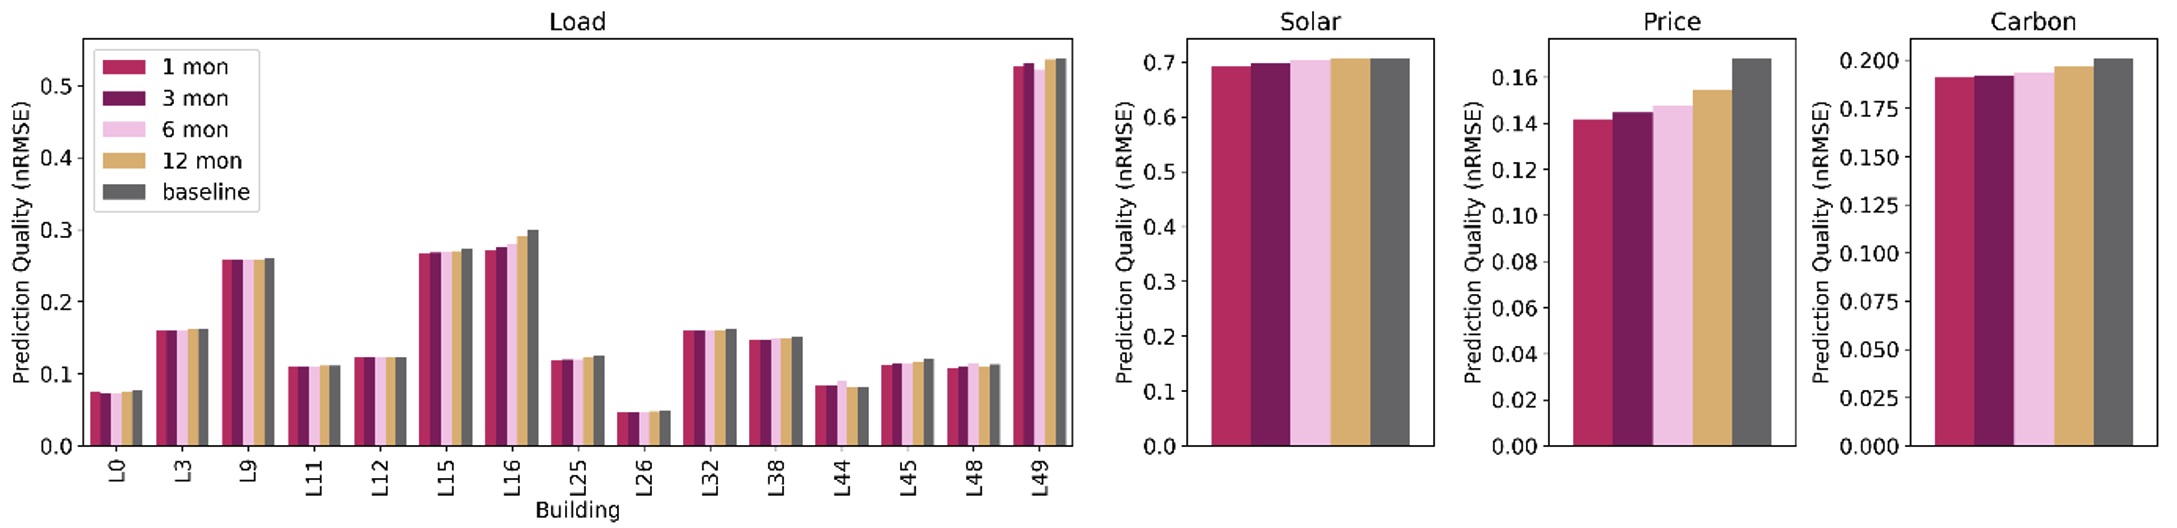
\includegraphics[width=\linewidth]{Data_Efficiency/prediction_vs_update_freq.png}
    \caption{Variation of prediction accuracy with online update frequency.}
    \label{fig:forecasting-data-eff-update-freq}
\end{figure}


\newpage
\subsection{Sensitivity of Model Predictive Control to forecast accuracy} \label{sec:forecasting-control-sensitivity}

% Tie forecasting analysis in with the simulation framework and explain how this provides a methodology for determining whether investment in additional data is economic -- e.g. model reuse vs direct data collection, data efficiency measures above, or purchase of external forecasts from service.
% May require some discussion about realism of noise model and correlation between results obtained and performance of true prediction models (grid performance poor for this synthetic noisy model which distorts results). But regardless this analysis provides an indicative method for how this type of economic analysis of optimal data requirements would be done. Opportunity for significant further work - create noise model calibrated to performance-accuracy trade-off of practical prediction models, which hopefully provides a better representation of the underlying inaccuracy patterns.

Whether investments in additional data to improve forecast accuracy provide net benefit to the operation of a smart energy storage system depends on the resulting improvements in operational performance achieved by the \glsxtrshort{mpc} controller. The determination of optimal data collection strategies therefore requires quantification of the relationship between forecast accuracy and \glsxtrshort{mpc} operational performance. To investigate this in a controlled setting, the operational performance achieved by the tested \glsxtrshort{mpc} scheme is evaluated with the use of synthetic forecasts. The synthetic forecasts are produced by adding a Gaussian random walk noise component to the ground-truth values, as described in Eq. \ref{eq:forecasting-GRWN},

\begin{equation} \label{eq:forecasting-GRWN}
    f_{\mathsmaller{\textrm{GRW}}}^v[t,\tau] = v_{t+\tau} + \sum_{j=1}^{\tau} w_j^{\sigma} \qquad \textrm{s.t.} \:\: w_j^{\sigma} \:\: \textrm{i.i.d.} \:\: \mathcal{N}\!\left( \mu{=}0, \sigma^2 \right)
\end{equation}

where $v_{t+\tau}$ is the ground-truth value of variable $v$ at instance $\tau$ in the planning horizon of the forecast created at time $t$, and the noise level $\sigma$ can be selected.

The \glsxtrshort{mpc} scheme using these synthetic forecasts for all prediction variables is tested at varying noise levels. Fig. \ref{fig:forecasting-control-sens-obj-vs-noise} shows the resulting operational performance of \glsxtrshort{mpc}, as well as the three components it is comprised of (electricity price, carbon emissions, and grid impact), as the prediction accuracy of the synthetic forecasts varies. Fig. \ref{fig:forecasting-control-sens-control-vs-noise-type} shows the variation in overall operational performance of the \glsxtrshort{mpc} when synthetic forecasts are used for each type of prediction variable in turn, with perfect forecasts used for all other variables. The horizontal line at 1 indicates the performance of the building energy system without battery control, which is the point at which the \glsxtrshort{mpc} controller becomes redundant.

The results show that the tested \glsxtrshort{mpc} scheme is most sensitive to the forecast accuracy of the grid electricity price and carbon intensity variables, suggesting that the most resource and expense should be invested in producing accurate forecasts of the grid conditions. Additionally, whilst the prediction models tested in this study performed worst when forecasting solar generation, see Fig. \ref{fig:forecasting-baseline-PCS-comparison}, it may not be worth expending additional resource to improve these forecasts as the \glsxtrshort{mpc} scheme is least sensitive to this variable. Though the grid component of operational performance is found to be by far the most sensitive to forecast accuracy, this is likely due to the synthetic forecast model used\footnote{In the synthetic forecast model used, the Gaussian random walk noise component is regenerated at each time instance. This leads to the generation of forecasts which are correct on average, but can cause the \glsxtrshort{mpc} controller to take opposing energy management strategies in successive time steps, leading to large magnitudes of energy flows from the battery to correct the strategy. Further work is required to create a noise model for synthetic forecasts that is calibrated to the operational performance vs forecast accuracy trade-off of practical prediction models. With such a noise model, the experimental method demonstrated could be used to quantify the economic advantage of forecast accuracy improvements to support decision making regarding data collection.} for the development of forecasting models in practical smart energy storage systems, and is not considered to be reflective of the behaviour of real prediction models.

\begin{figure}[p]
    \centering

    \subfloat[Variation of operational performance components with amplitude of noise on all prediction variables.]{
        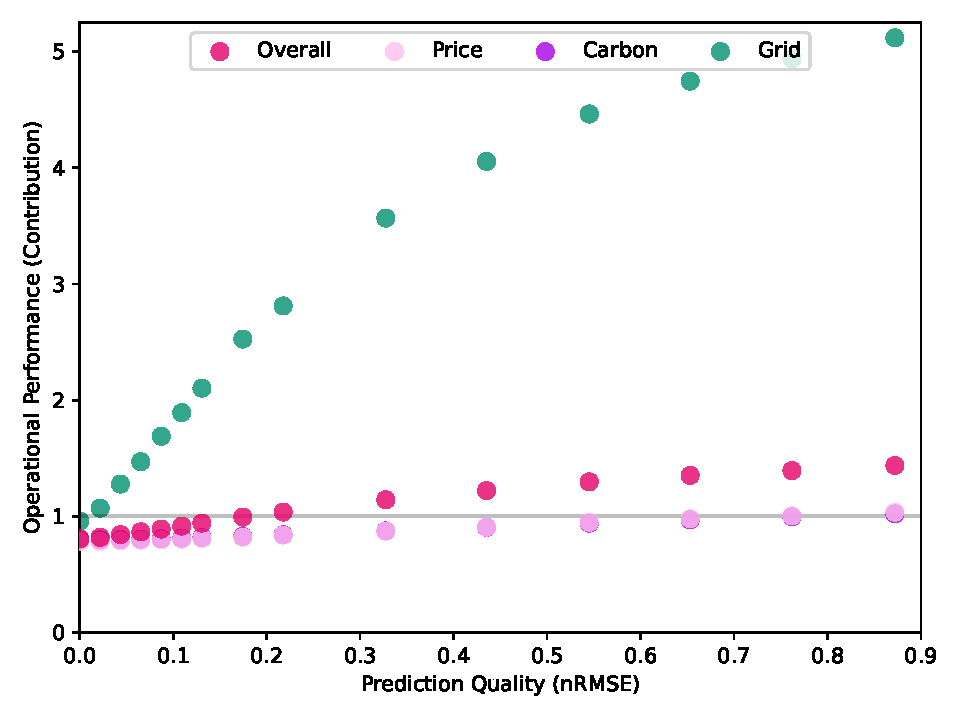
\includegraphics[width=0.7\linewidth]{Control_Sensitivity/control_obj_vs_noise.pdf}
        \label{fig:forecasting-control-sens-obj-vs-noise}
    }
    \bigskip

    \subfloat[Variation of overall operational performance with amplitude of noise on each type of prediction variable.]{
        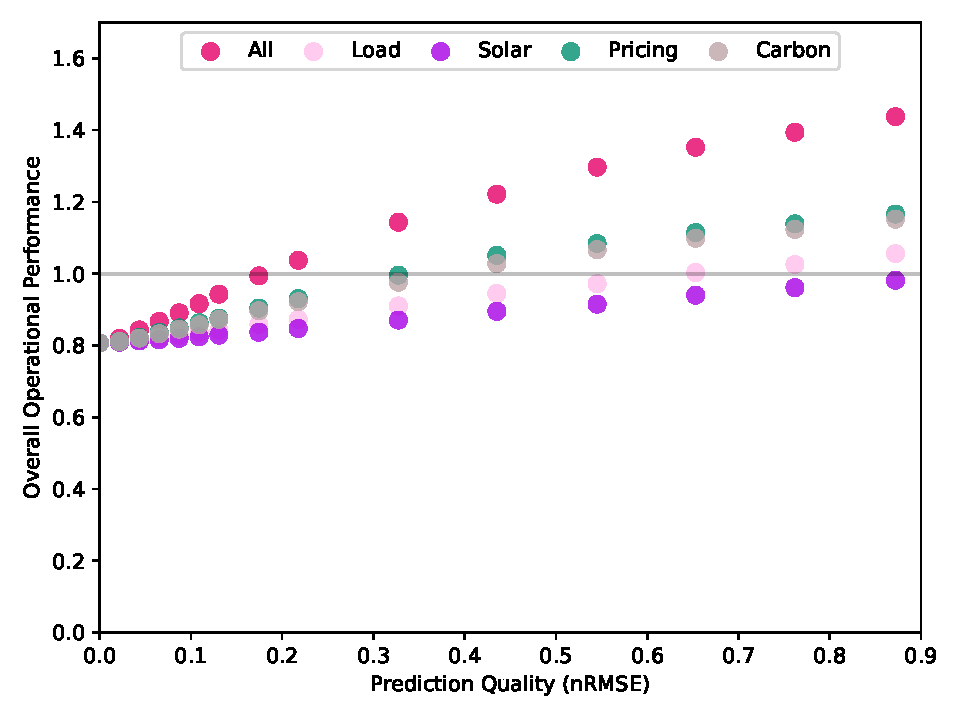
\includegraphics[width=0.7\linewidth]{Control_Sensitivity/control_performance_vs_noise_type.pdf}
        \label{fig:forecasting-control-sens-control-vs-noise-type}
    }
    \smallskip
    \caption{Sensitivity of operational performance to synthetic forecast noise simulating prediction inaccuracy.} \label{fig:forecasting-control-sens}
\end{figure}


\newpage
%********************************** Conclusions **************************************
\section{Conclusions} \label{sec:forecasting-conclusions}

This chapter investigated the impacts of data on the accuracy of machine learning based forecasting models for building operational conditions, and the resulting operational performance of a \glsxtrlong{mpc} (\glsxtrshort{mpc}) scheme in a multi-building energy system with distributed generation and storage. Experiments were conducted using a large-scale dataset of electrical load measurements from buildings in the Cambridge University Estates.

A simple linear multi-layer perceptron model (Linear) using DMS prediction was found to achieve equivalent forecast accuracy to high-complexity, state-of-the-art machine learning models in a setting without data limitations, but has substantial advantages regarding data efficiency and generalisation performance. So, this simple neural model is better suited for use in practical \glsxtrshort{mpc} systems due to its lower data and computational requirements, and better performance on new load dynamics.

Using more than 2 years of hourly resolved training data did not provide significant improvements in prediction accuracy for most of the models tested, indicating that the collection of monitoring data for longer durations is unnecessary for the development of performant \glsxtrshort{mpc} schemes. Further, screening training data using change-point analysis to remove low similarity data was able to simultaneously improve data efficiency and prediction accuracy, provided at least 1 year of training data was kept. This could also be achieved through the removal of redundant data features from models.

The reuse of Linear models for load prediction between buildings was shown to be an effective way of reducing data collection requirements. When selecting models for reuse using a proposed load profile similarity metric based on the Wasserstein distance between fPCA coefficient distributions, model reuse led to an average 11\% increase in prediction error. However in comparison, models trained using only 3 months of building specific data provided forecasts with an average 9.9\% increase in error compared to the baseline. Additionally, online training of prediction models was shown to be highly beneficial, with higher update frequencies providing greater forecast accuracy improvements, of up to 15.7\% for the case of monthly updating. Hence, monitoring data should be used to update reused prediction models in situ to tailor them to the building system, ultimately replacing the reused model. The results suggest that, by exploiting existing building energy datasets to pre-train models, in many cases sufficient forecast accuracy can be achieved without the collection of any building load data prior to the installation of the system.

The relationship between forecast accuracy and operational performance of the \glsxtrshort{mpc} controller was investigated for synthetic forecasts, which showed the \glsxtrshort{mpc} scheme is most sensitive to grid electricity price and carbon intensity prediction accuracy. This indicates that the most effort and expense should be spent on developing or purchasing high accuracy forecasts of the grid conditions, as these will provide the greatest improvement in operational performance of the controller.

% In some sense you can think of gathering more data as reducing uncertainty in the building behaviour, but it's very difficult to come up with a statistical model of this, so VoI isn't super appropriate - in fact from what we've seen, more data doesn't always lead to improvements in performance. We need to be a little bit more anecdotal, as this is a pretty complex data setting
% Comparison of general/foundation models vs building specific models is explored in the project with Fabian

In this chapter, the operational performance of the \glsxtrshort{mpc} controller was studied using a relative performance metric\footnote{This was done to match the goal of the CityLearn Challenge 2023 \citep{nagy2023CityLearnChallenge2023}.}. However, the analysis could be repeated using an economic performance metric. This would allow the financial benefit of data for improving forecast accuracy to be quantified. By comparing to the costs of data collection, building operators could determine whether expenditure on additional data collection or commercial forecasts is beneficial, i.e. whether the costs of data are outweighed by the improvements in operational performance provided. And if so, the results could also be used to determine the optimal data collection strategy.

This analysis would be conceptually quite similar to a \glsxtrlong{voi} analysis, and has the same objective. However in this case using the \glsxtrshort{voi} methodology is not appropriate. While collecting more training data could be viewed as reducing uncertainty in the behaviour of a building, it is not clear how a statistical model of this uncertainty could be constructed, and whether the setup is really compatible with a statistical viewpoint\footnote{Data collected other buildings could be viewed as a prior distribution for the load data of the target building. This is the modelling approach taken in \Cref{chap:districts}. A prediction model trained on this data, often referred to as a general or foundation model, could be seen as a prior decision. This general model could then be updated using data collected from the target building in a Bayesian-like fashion, improving prediction accuracy for the target building. An approach similar to this is taken in \citep{raisch2025AdaptingChangeComparison} to study the impact of data on the accuracy of system dynamics models.}.
The analysis in \Cref{sec:forecasting-data-efficiency} showed that collecting more data does not always improve prediction accuracy, as building load dynamics can change over time, and additional historic data is not always representative of the current behaviour, meaning it can worsen model training. This breaks one of the key assumptions of the \glsxtrshort{voi} methodology. An analysis using synthetic data could be performed, however it would be difficult to justify or validate its applicability to real-world energy systems.
So due to the complexity of the data required to study forecasting accuracy, the case study based approach used in this chapter is better suited for investigating data collection requirements for forecasting.


\newpage
%********************************** Chapter appendices  **************************************
\begin{subappendices}
    \section{Multi-building energy system asset specification} \label{app:forecasting-system-spec}

    The specifications of the distributed generation and storage assets for the multi-building energy system simulated in this study are provided in Table \ref{tab:forecasting-energy-assets}. The battery power capacities are set to be 3 times the mean building electrical load in the test dataset, the battery energy capacities are set to be able to provide 24 hours of that mean electrical load, and the solar PV power capacities are set by assuming 90\% of the roof area of each building is filled by solar panels of power density 0.15 kWp/m$^2$.\\

    \begin{table}[h]
        \centering
        \renewcommand{\arraystretch}{1}
        \begin{tabularx}{\linewidth}{c|*{4}{>{\setlength{\baselineskip}{.5\baselineskip}}Y}} \toprule \toprule
            Building & Battery power capacity (kW) & Battery energy capacity (kW) & Battery efficiency (\%) & Solar PV power capacity (kWp) \\ \midrule
            0 & 531 & 4246 & 90 & 461 \\
            3 & 60 & 478 & 90 & 38 \\
            9 & 14 & 108 & 90 & 20 \\
            11 & 342 & 2736 & 90 & 41 \\
            12 & 98 & 780 & 90 & 89 \\
            15 & 203 & 1622 & 90 & 143 \\
            16 & 306 & 2448 & 90 & 120 \\
            25 & 275 & 2198 & 90 & 118 \\
            26 & 1001 & 8006 & 90 & 136 \\
            32 & 157 & 1255 & 90 & 166 \\
            38 & 58 & 461 & 90 & 46 \\
            44 & 1084 & 8674 & 90 & 663 \\
            45 & 1245 & 9962 & 90 & 437 \\
            48 & 622 & 4973 & 90 & 500 \\
            49 & 57 & 458 & 90 & 258 \\
            \bottomrule\bottomrule
        \end{tabularx}
        \smallskip
        \caption{Specification of distributed energy assets in simulated multi-building energy system.}
        \label{tab:forecasting-energy-assets}
    \end{table}


    \newpage
    \section{\glsxtrshort{mpc} planning horizon} \label{app:forecasting-tau}

    % Provide references and plot to justify use of $\tau=48$ - good trade-off of near-optimal control performance and feasible computation time (+ no failures)

    The planning horizon used in a \glsxtrshort{mpc} scheme determines its ability to effectively arbitrage energy and meet the operational objectives of energy management. Previous studies show that a planning horizon of 24 hours is sufficient when controlling HVAC systems \citep{oldewurtel2012UseModelPredictive}, and recommend 48 hours as a suitable value for systems with distributed solar and storage \citep{thieblemont2017PredictiveControlStrategies}.

    To demonstrate the suitability of a planning horizon of $T=48$hrs for the experiments on the test system in this study, the operational performance of the \glsxtrshort{mpc} scheme using perfect forecasts is evaluated over varying planning horizon lengths, along with the computational time required to solve the Linear Programs for the simulations, shown in Fig. \ref{fig:forecasting-planning-horizon}. It can be seen that $T=48$hrs provides near-optimal control performance at a reasonable computation time, and so is a suitable choice for the experiments.\\

    \begin{figure}[h]
        \centering
        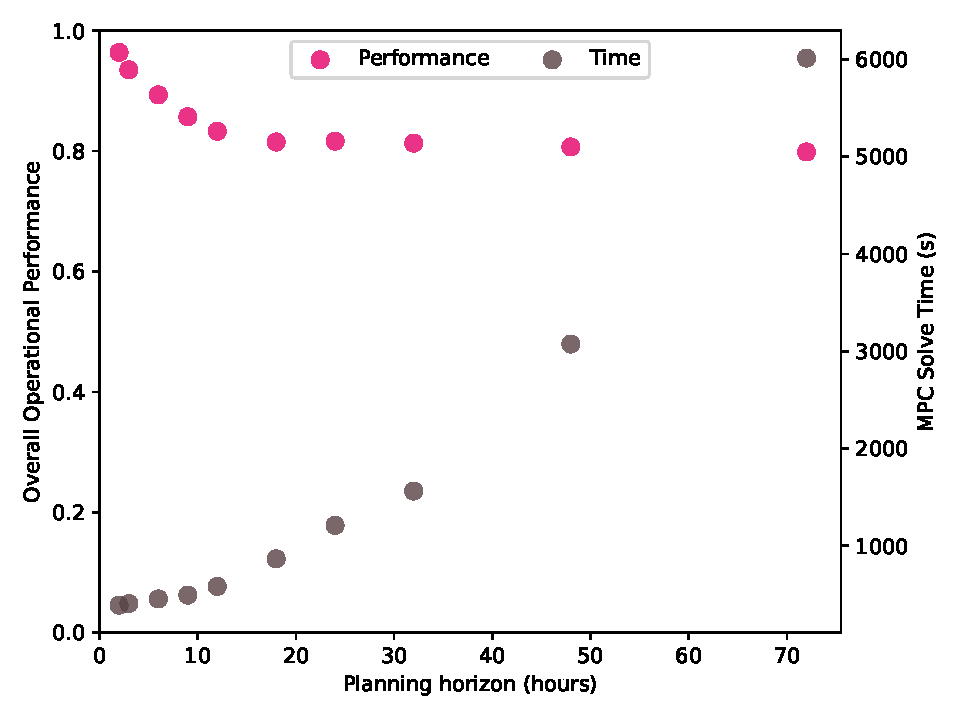
\includegraphics[width=0.6\linewidth]{Appendices/planning_horizon.pdf}
        \caption{Variation of perfect forecast \glsxtrshort{mpc} operational performance and computation time with planning horizon, $T$.}
        \label{fig:forecasting-planning-horizon}
    \end{figure}


    \newpage
    \section{Technical specification of prediction models and training procedures} \label{app:forecasting-models}

    % Provide references to package documentation for model implementations and training procedure.

    The model parameters and training procedure used for machine learning models have a significant impact on their performance, as well as their computational and data requirements. Hence, they must be selected carefully for the target application to maximise model performance with the available computational resources and data.

    \subsection{Simple neural models}

    For the simple neural models, implementations from the Pytorch Lighting library \citep{falcon2019PyTorchLightning} were used. The models use an input window of 168 time steps (input dimension) and output a forecast of 48 time steps (output dimension). All models were trained using the Adam optimizer \citep{kingma2017AdamMethodStochastic}, with a batch size of 32 and a learning rate determined using the built-in learning rate tuner.

    The Linear model consists of a single linear layer, of size 48, with no activation function used.

    The Convolution model uses two 1D convolution layers with channels (5, 1) and kernel sizes (5, 6), respectively, with ReLU activation functions. This is followed by an output MLP that brings the dimensionality to 48.

    The ResMLP model has an linear layer with 168 nodes, using a residual connection and ReLU activation. A subsequent output linear layer brings the dimensionality to 48.

    \subsection{State-of-the-art machine learning models}

    For the complex, state-of-the-art models, implementations from the Pytorch Forecasting library \citep{beitner2024Jdb78Pytorchforecasting} were used. The models take in data from the previous 72 time steps along with known covariate data from the coming 48 time steps, and output forecasts of the target variable for the coming 48 time steps. All models were trained using an early stopping trainer with a patience of 5, for a maximum of 50 epochs, with a limit of 800 training batches per epoch. The learning rate was determined using the built-in learning rate tuner. The size parameters, loss functions, and optimizers used are detailed in Table \ref{tab:complex-model-specs}.

    \begin{table}[h]
        \centering
        \renewcommand{\arraystretch}{1}
        \begin{tabularx}{\linewidth}{c|*{3}{>{\setlength{\baselineskip}{.5\baselineskip}}Y}} \toprule \toprule
            Model & TFT & NHiTS & DeepAR \\ \midrule
            Hidden size & 48 & 128 & 64 \\
            Drop-out & 0.1 & 0.1 & 0.1 \\
            Loss & Quantile loss & Quantile loss & Normal distribution loss \\
            Optimizer & Adam & AdamW & Adam \\[1ex]
            & \makecell{Attention head size: 4}
            & \makecell{Weight decay: 0.01\\Backcast loss ratio: 0}
            & \makecell{RNN layers: 3} \\
            \bottomrule\bottomrule
        \end{tabularx}
        \smallskip
        \caption{Technical specifications of complex, state-of-the-art models.}
        \label{tab:complex-model-specs}
    \end{table}


    \newpage
    \vspace*{0cm}
    \section{Data similarity metric} \label{app:forecasting-similarity-metric}

    \subsection{Functional data analysis}

    Functional Data Analysis (FDA) is used to analyse and compare the energy usage behaviours across the building electrical load dataset of 15 buildings. In this approach, functional principal components (fPCs) are extracted from the data, such that each data sample can be constructed from an equation of the form,

    \begin{equation}
        f(t) = \mu(t) + \sum_{i=1}^n \alpha_i \nu_i(t)
    \end{equation}

    i.e. the data sample, $f(t)$, is constructed from a linear sum of a mean function, $\mu(t)$, and a weighted sum of $n$ fPCs , $\nu_i(t)$, with weightings or `scores' $\alpha_i$. The mean function and fPCs are the same across all data samples, whereas the weightings are unique to each data sample. This has the benefit that to compare data samples, which are functions of time, it suffices to compare the weightings, a low-dimensional representation of the functional data, that can be analysed using standard statistical techniques.

    For this analysis, the datasets are pre-processed into daily time histories, such that each data sample is a 24 hour profile of electricity consumption, starting at midnight. For each building, the training dataset comprises 6 years of data and hence 2191 data samples, and the validation and test datasets are both 2 years and hence 731 and 730 data samples respectively (2016 was a leap year).

    The functional Principal Component Analysis (fPCA) approach used involves first aligning the data samples to a common mean, $\mu(t)$. This generates a warping function and an amplitude function for each data sample that describe how the data sample maps to the mean function. The warping function describes the phase relationship, i.e. the variation in time, and the amplitude function describes changes in magnitude. The warping and amplitude functions are then analysed separately and fPCs generated for both. The approach is illustrated schematically in Fig. \ref{fig:forecasting-fPCA-method}, and full details of the approach are described in (Ward, 2021) \citep{ward2021DatacentricStochasticModel}.

    Fig. \ref{fig:forecasting-fPC-effects} illustrates the first two phase and amplitude fPCs extracted from the dataset. Fig. \ref{fig:forecasting-fPCs-scatter} shows distributions of example fPC coefficients for Buildings 38 and 49. The load data for Building 49 exhibits a much lower range than that for Building 38, which results in a more positive distribution of V1 fPC coefficients. In Fig. \ref{fig:forecasting-fPC-effects} positive coefficients V1 fPC can be seen to reduce the data range.

    \begin{figure}[p]
        \centering
        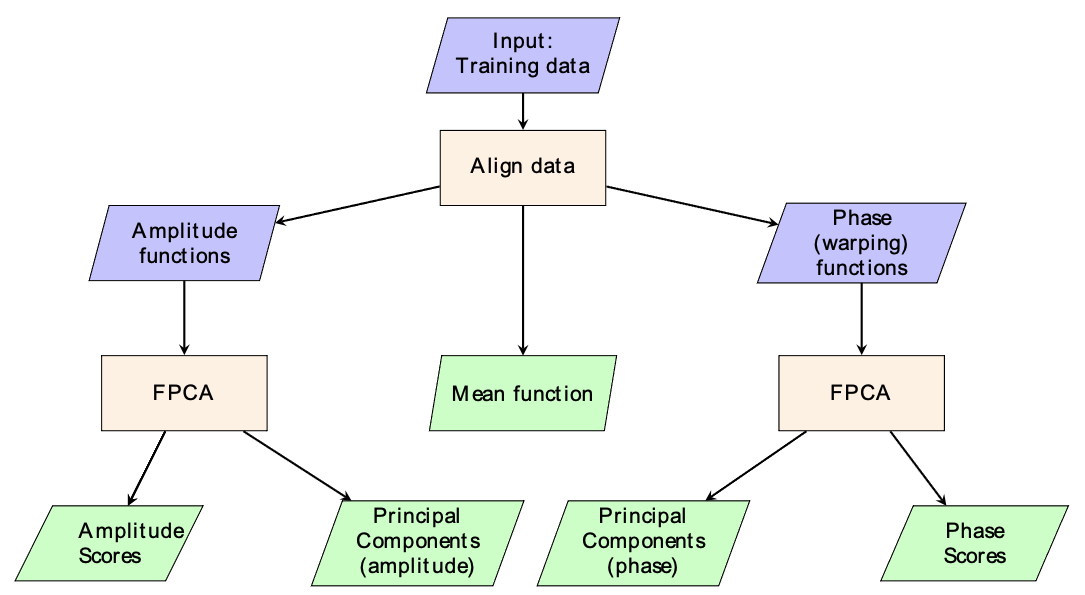
\includegraphics[width=0.6\linewidth]{Data_Analysis/fPCA-flow-diag.png}
        \caption{Schematic process for functional principal component analysis (fPCA)}
        \label{fig:forecasting-fPCA-method}
    \end{figure}

    \begin{figure}[p]
        \centering
        \begin{minipage}{.525\textwidth}
            \centering
            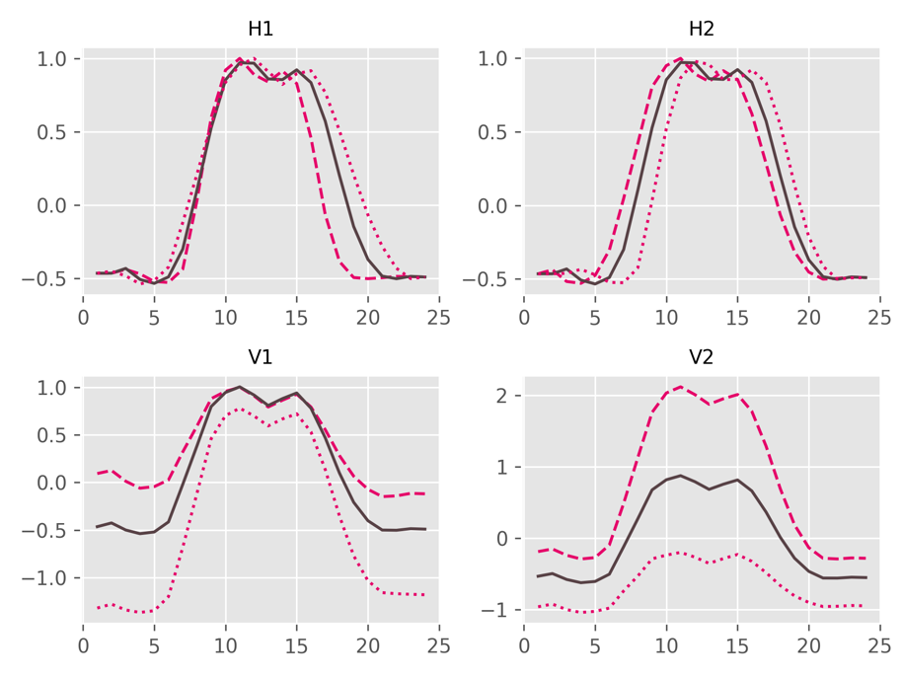
\includegraphics[width=0.9\linewidth]{Data_Analysis/fPC-effects.png}
            \caption{Illustration of first two Phase (H) and Amplitude (V) fPCs. Solid black line shows mean function, $\mu(t)$. Dashed line (-) indicates the impact of a +ve coefficient and dotted line (.), a -ve coefficient.}
            \label{fig:forecasting-fPC-effects}
        \end{minipage}%
        \hfill
        \begin{minipage}{.425\textwidth}
            \centering
            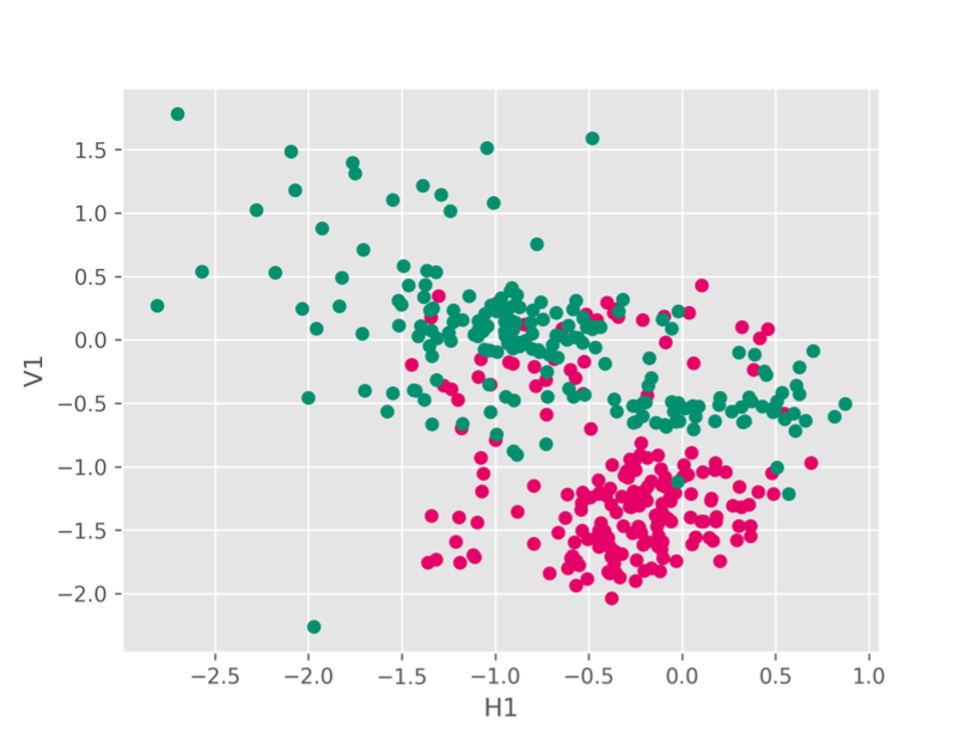
\includegraphics[width=\linewidth]{Data_Analysis/fPC-scatter.png}
            \caption{Example fPC coefficient distributions for Buildings 38 (pink) and 49 (green)}
        \label{fig:forecasting-fPCs-scatter}
        \end{minipage}%
    \end{figure}

    % Move here to get data analysis figures on a page
    \begin{figure}[p]
        \centering
        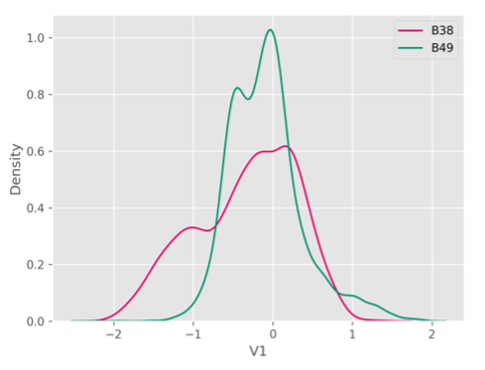
\includegraphics[width=0.4\linewidth]{Data_Analysis/fPC-dist-comparison.png}
        \caption{Kernel density plot of V1 scores for Buildings 38 \& 49. Wasserstein distance between two distributions is 0.05.}
        \label{fig:forecasting-fPC-comparison}
    \end{figure}

    \subsection{Wasserstein similarity metric} \label{forecasting-similarity-metrics}

    The deconstruction of the data into fPCs and corresponding coefficients enables the use of standard statistical techniques to define measures of similarity between load profiles in the dataset. A load profile similarity metric based on an optimal transport approach is proposed. This metric is based on the approximate Wasserstein distance, or Earth-mover's distance, between the distributions of PC coefficients, which provides a measure of the ease with which one probability distribution can be transformed into the other, and hence is a measure of the similarity of the two distributions. As such, the metric is referred to as the `Wasserstein similarity metric', and is computed using the \href{https://github.com/jeanfeydy/geomloss}{Geomloss} \citep{feydy2024JeanfeydyGeomloss} library. Advantages of this method are that it provides a comparison of the underlying patterns in the load profiles that is not excessively distorted by sequence misalignments as is the case for simple metrics like RMSE, and it allows time series of different durations to be compared.

    % Q: what's approximate about the calculation? A: It's a complex calculation and the methodology purports to give an approximate solution
    % Q: What specifically is the metric? The average Wasserstein distance over all fPCs? A: It is the distance between one multivariate distribution and another.  So it is the distance between sets of PC coefficients.  

    Fig. \ref{fig:forecasting-fPC-comparison} shows the kernel density distributions of the V1 fPC coefficients for Buildings 38 and 49. The Wasserstein distance between these distributions is 0.05. Similarity metric values are computed for comparison of the training datasets between pairs of buildings, and for the comparison of pairs of training, validation, and test datasets for each building individually. Figures \ref{fig:forecasting-similarities-buildings} \& \ref{fig:forecasting-similarities-datasets} provide the results of these similarity metric calculations.

    \begin{figure}
        \centering
        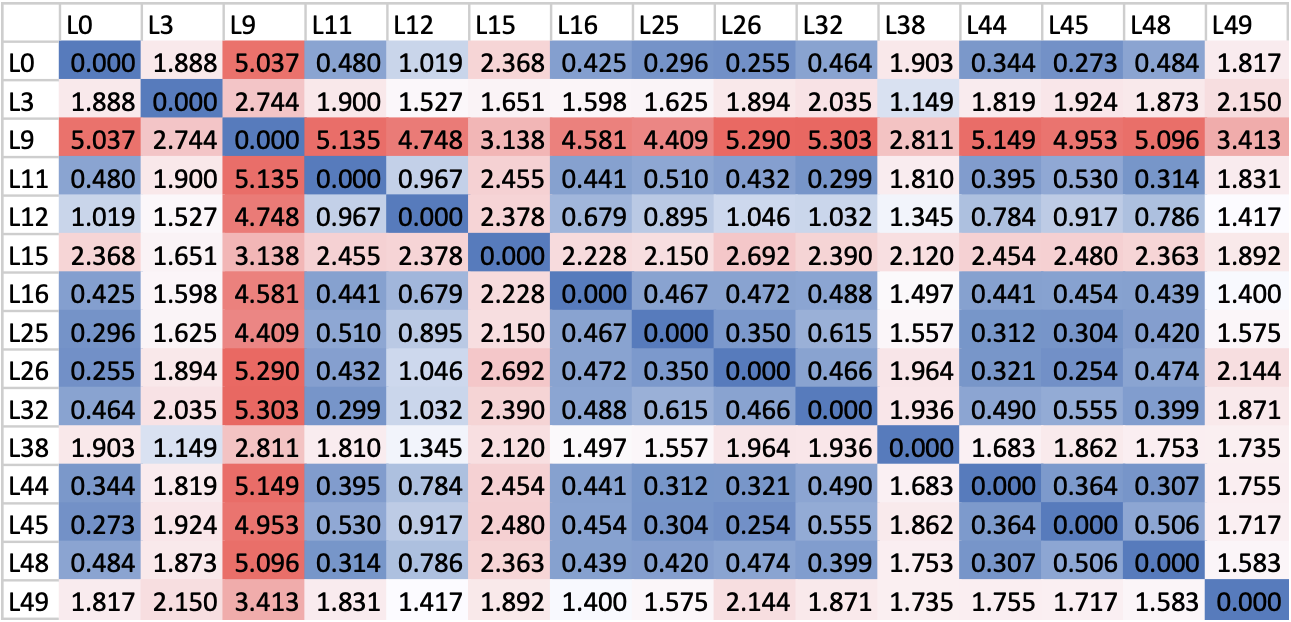
\includegraphics[width=0.8\linewidth]{Data_Analysis/building-similarities.png}
        \caption{Similarity metric scores between training datasets for pairs of buildings.}
        \label{fig:forecasting-similarities-buildings}
    \end{figure}

    \begin{figure}
        \centering
        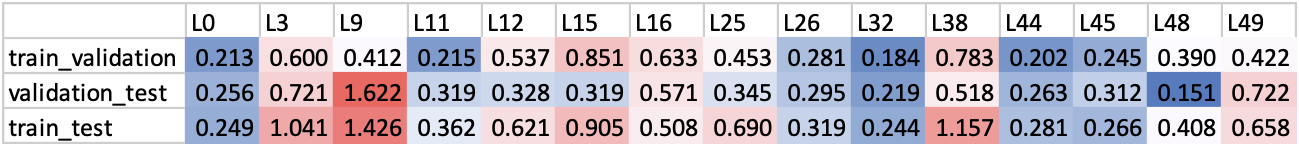
\includegraphics[width=0.8\linewidth]{Data_Analysis/data-similarities.png}
        \caption{Similarity metric scores between pairs of training, validation, test datasets for each building.}
        \label{fig:forecasting-similarities-datasets}
    \end{figure}

    % A similarity metric is proposed to enable the efficient comparison of load profiles.
    % The potential of this metric to provide a data analysis based methodology for estimating prediction model generalisation performance is investigated in Section 7.


    \newpage
    \vspace*{0cm} % classic tex jank
    \section{Change-point analysis} \label{app:forecasting-change-points}

    Building electrical loads are driven by occupancy behaviour dynamics which span timescales: seasonal (winter heating vs. summer cooling loads), weekly (inhabitance trends due to working patterns, i.e. weekday vs. weekend), and daily (nighttime vs. daytime). The form of these behavioural trends also differs between buildings depending on their usage, e.g. offices and residential buildings have opposing daily trends. Gradual changes can occur in these behavioural trends, for instance due to cultural shifts in working patterns. Alternatively, abrupt changes can be caused by severe disturbances, such as building stock refurbishment, temporary vacancy, or occupant behavioural changes due to change in building use. As such, changes can occur in the seasonal and/or trend patterns of building load time series, and the underlying patterns of the dynamics can differ significantly following disturbances.

    This raises the question as to whether all historic measurement data is useful for the training of load prediction models, as the underlying patterns in certain sections of the historic data may differ significantly from the current behaviour of the building load, i.e. be non-representative. Including these sections in the training dataset may poison model training, leading to worse prediction performance.

    \begin{figure}[t]
        \centering
        \hspace*{\fill}
        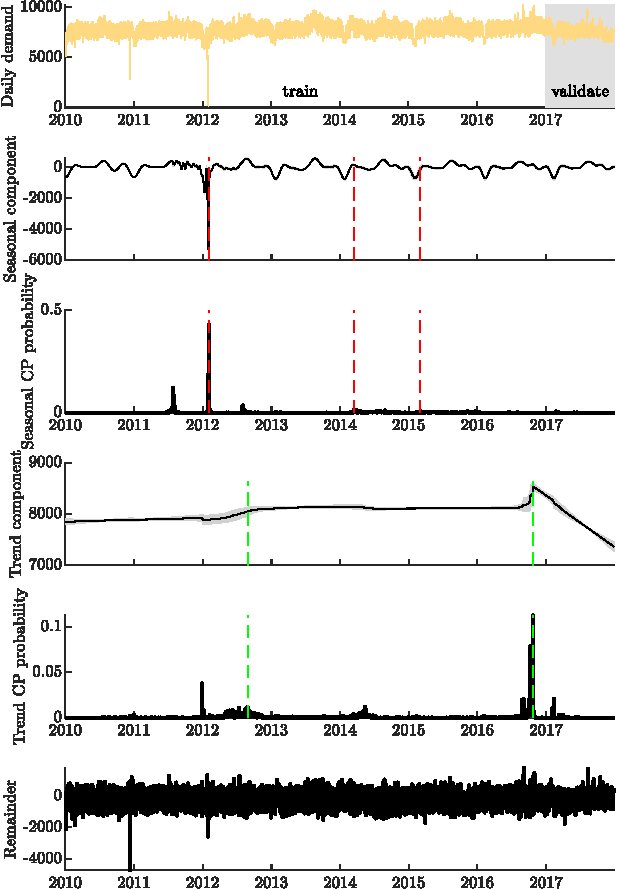
\includegraphics[width=0.45\linewidth]{Changepoint/Annexe37_CPoutput_B26_eps-conv.pdf}
        \hspace*{\fill}
        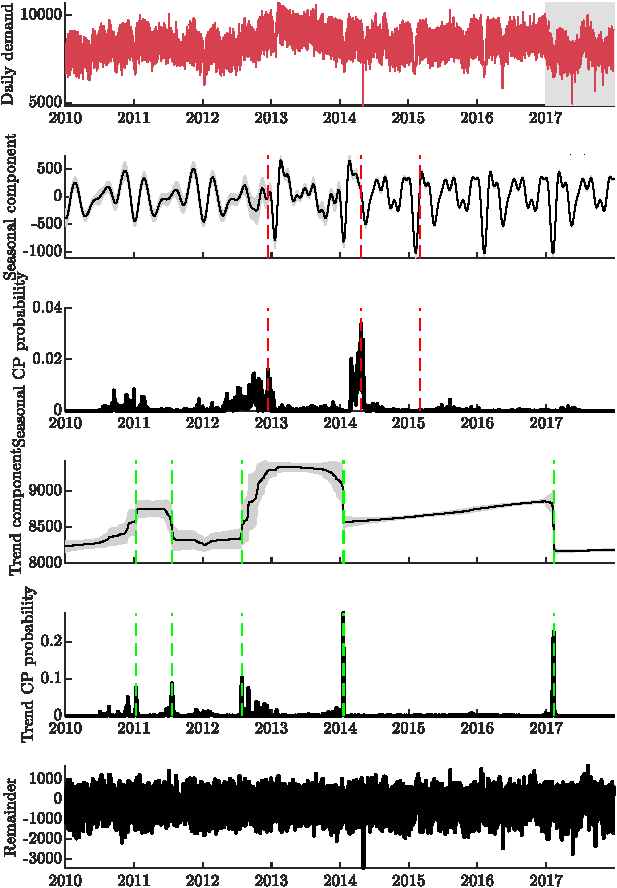
\includegraphics[width=0.45\linewidth]{Changepoint/Annexe37_CPoutput_B44_eps-conv.pdf}
        \hspace*{\fill}
        \bigskip
        \caption{Change-points detected using the BEAST algorithm in load profiles of Buildings 26 \& 44 (top row). Signal is decomposed into a seasonal component (second row), assumed harmonic, inferred change-points indicated by red vertical lines, and a trend component (fourth row), with green lines indicating change-points. Credible intervals of the estimated signals are given by grey envelopes around the individual components.}
        \label{fig:forecasting-change-points}
    \end{figure}

    A change-point analysis is conducted on the building electrical load dataset to detect changes in the load patterns in each building. The Bayesian ensemble algorithm ``Bayesian Estimator of Abrupt change, Seasonal change, and Trend'' (BEAST) \citep{zhao2019DetectingChangepointTrend} is used to decompose the load time series and derive non-linear dynamics across multiple timescales, detecting change-points, seasonality, and trends. The value of this ensemble approach is that it quantifies the relative usefulness of individual decomposition models, leveraging all the models via Bayesian model averaging. Additionally, it provides an estimated probability of inferred change-points being `true’ change-points. Results of the change-point analysis for Buildings 26 \& 44 are shown in Fig. \ref{fig:forecasting-change-points}. The demand profiles are decomposed into seasonal and trend components, and detected change-points for the two components are indicated in red and green respectively. The trend component of Building 44 is found to vary substantially more than that of Building 26, which corresponds with the visual variability of the demand profiles.
\end{subappendices}
\cleardoublepage
%!TEX root = ../thesis.tex
%*******************************************************************************
%*********************************** District energy systems chapter *****************************
%*******************************************************************************

\chapter[Supporting solar-battery system sizing with load monitoring]{Supporting solar-battery system sizing with\\load monitoring} \label{chap:districts}

\graphicspath{{Districts/Figs/}}

\begin{cbox}{}
    \printpublication{langtry2025QuantifyingBenefitLoad}

    \noindent{\color{black!50}\rule{\textwidth}{0.4mm}}\vspace{2mm}

    \noindent
    This chapter has been published as the journal article above.\\

    \noindent
    All code and data used to perform the experiments in this chapter is available at \url{https://github.com/mal84emma/Building-Design-VoI}.
\end{cbox}

\newpage

%********************************** Graphical abstract **************************************
\begin{figure}
    \centering
    \includegraphics[width=\textwidth]{districts_graphical_abstract.pdf}
    \caption{Graphical abstract of \Cref{chap:districts}.}
    \label{fig:districts-district_graphical_abstract}
\end{figure}
\hfill \\
%********************************** end **************************************

\vspace{0.5cm}

\noindent
When building energy systems are designed there is substantial uncertainty in how much energy the building will actually use, and how that energy usage will look. This load uncertainty needs to be accounted for during design to make sure the building energy system can both meet the building's energy needs and manage its impact on the grid.
Reducing uncertainty in building load allows for improved designs with less compromise to be identified, reducing the cost of decarbonising the building's energy usage. However, monitoring the building and gathering the data required to reduce load uncertainty at the time the energy system is designed is costly.
This chapter quantifies the economic value of practical monitoring data for improving the design of building energy systems, to determine whether the benefits of reducing load uncertainty outweigh the costs.
The On-Policy \glsxtrshort{voi} framework from \Cref{sec:methodology-on-policy-voi} is applied to a case study district energy system design problem. This case study uses a Linear Program model to size solar-battery systems and grid connection capacity under uncertain building loads, which are modelled using historic electricity metering data from the Cambridge University estate.
The chapter investigates the impact that the building load uncertainty has on the performance of the district energy system, and the impact that reducing that uncertainty has on the system design.

\newpage
%********************************** Intro section **************************************
\section{Introduction}

Many countries such as the UK and EU have implemented policies focusing on the adoption of heat pumps to decarbonise building heating through electrification \citep{houseofcommons2022DecarbonisingHeatHomes,iea2021NetZero2050}. However, achieving a widespread roll-out of heat pumps comes with significant challenges for decarbonising building electricity usage and managing the electrical grid.
Electrifying heating will substantially increase the total demand for electricity, and more significantly peak electricity demand \citep{heinen2018HeatElectrificationLatest}, which would rise by 50\% in the UK \citep{zhang2022AssessmentImpactsHeat,charitopoulos2023Impact100Electrification}. Supporting this additional electricity demand while maintaining security of supply requires investment in distribution and transmission systems \citep{blonsky2019PotentialImpactsTransportation}, as well as reserve generation capacity \citep{charitopoulos2023Impact100Electrification}, which add to the cost of heat decarbonisation.
Already, capacity limitations on the electrical supply system are causing delays to both building construction and renewable power generation projects \citep{beis2023PoweringBritain,departmentforbusinessandtrade2023UKBatteryStrategy}, and it is widely acknowledged that network capacity limitations are a significant barrier to future decarbonisation \citep{haben2023ADViCEAIDecarbonisation}.

To achieve 2050 decarbonisation targets, energy retrofits must be cheap enough so that they are widely adopted, but also able to be safely integrated into the wider energy system. This means building energy systems must be designed to balance their total system cost, the carbon emissions reductions they achieve, and their impact on the electrical grid.
The installation of distributed generation and storage in buildings has become a popular route to reducing the carbon emissions of building energy usage, and so has attracted considerable research attention in recent years \citep{li2023ReviewPhotovoltaicBattery,niveditha2022OptimalSizingHybrid,sharma2020EconomicPerformanceAssessment,novoa2019OptimalRenewableGeneration,salvador2012MethodologyDesignEnergy,tumminia2020GridInteractionEnvironmental}.
This is due to the falling costs of solar PV generation \citep{irena2023RenewablePowerGeneration}, and the need for local storage to both improve buildings' utilization of the solar energy and reduce the grid impact caused by peaks in solar generation \citep{li2023ReviewPhotovoltaicBattery}.

When designing building energy systems, there is substantial uncertainty concerning the conditions in which they will operate. This includes weather conditions which affect local energy generation, building usage type and occupant behaviour which determine the timing of energy usage, and building envelope characteristics which influence the building thermal response.
Of particular importance for managing grid impacts is the electricity usage behaviour of a building, including the timing and magnitude of peak loads. Due to the greater weather dependence and seasonal variability of heating loads, electrification of heating will increase uncertainty in building electricity usage \citep{deroubaix2021LargeUncertaintiesTrends,egging-bratseth2021SeasonalStorageDemand}, in terms of both the aggregate and peak demand.
The challenges posed by these uncertainties, and methods for properly accounting for them during the design of building energy systems have been widely studied \citep{zhu2022UncertaintySensitivityAnalysis,decarolis2017FormalizingBestPractice,fodstad2022NextFrontiersEnergy,mavromatidis2018ReviewUncertaintyCharacterisation,tian2018ReviewUncertaintyAnalysis}.

There are two routes to improve the design, and so eventual operational performance, of future decarbonised building energy systems. Firstly, improving optimisation methods for designing energy systems in the presence of uncertainties. Secondly, reducing the uncertainty in the conditions in which the energy system will operate, by for example monitoring the heating and electricity use patterns of the building prior to designing the heating retrofit. Optimisation methodologies have received concerted research effort for many years \citep{connolly2010ReviewComputerTools,fodstad2022NextFrontiersEnergy}, whereas there has not yet been any study of the potential benefits of uncertainty reduction for improving energy system design.

Reducing uncertainty in the operational conditions of a building improves energy system design by allowing a design that is better tailored to actual needs of the building to be identified, i.e. one with less hedging/compromise. So uncertainty reduction can lower the cost of decarbonising the building's energy usage.
However, uncertainty reduction is itself costly. For the case of existing buildings, these costs arise from the hardware and software needed to monitor energy consumption patterns, and the cost of management, curation, analysis, and interpretation of the data.
In the UK, only 51\% of electricity and gas meters are currently `smart' (able to collect hourly energy usage data), despite rollout beginning in 2012, and expected to cost £19.4bn in total \citep{desnz2023UpdateRolloutSmart}.
So it is important to quantify the benefit that uncertainty reduction via monitoring buildings provides to energy system design. Specifically, whether the reductions in total system cost are greater than the cost of gathering and exploiting the data needed to reduce uncertainty.


\subsection{Quantifying the impacts of uncertainty on building energy system design}

As discussed in the \nameref{chap:introduction}, the impact that uncertainties in buildings have on the performance of energy systems, and methods for accounting for and managing these uncertainties during system design, have been studied extensively (see \Cref{sec:uncertainty-methods-lit}).
However, there has been very little study of the impact these uncertainties have on the process of designing building energy systems.

A few previous studies have investigated the influence uncertainties have on the optimal system design.
\citep{sun2015SensitivityAnalysisMacroparameters} analyses the design of a Net Zero Energy Building with distributed generation and storage, and plots how the capacities of each system component (chillers, wind turbines, solar panels, and battery) and the total cost of the optimized system change with uncertain values of properties of the building (including wall thickness, internal heat gain, temperature set point). Additionally, influence coefficients of the uncertain parameters are computed for the capacity of each system component. A later study, \citep{sanajaobasingh2018ModelingSizeOptimization}, performed a similar analysis for another system with distributed generation and storage, investigating how the optimal design and total cost changed with varying scenarios of renewable generation. In both cases no statistical distributions of the uncertain parameters were considered, and so the insights gained are limited. For example, in the case of \citep{sanajaobasingh2018ModelingSizeOptimization}, it is unclear whether a design with a substantially greater number of PV panels is likely to be optimal, and so worth investing in.

A statistical \glsxtrlong{sa} for the optimal design of an energy system with distributed generation and storage was performed in \citep{mavromatidis2018UncertaintyGlobalSensitivity}. In this study, a Mixed Integer Linear Program was used to optimize the sizing of boilers, heat pumps, thermal storage, and PV generation for scenarios defined by samples from distributions of uncertain parameter values, including energy and capital costs, conversion efficiencies, and energy demand. This enabled a distribution of optimal sizes to be created for each component to illustrate how the uncertainties affect the optimal design choice. \citep{pickering2019DistrictEnergySystem} performed a similar procedure for the sizing of components in a district energy system, however the optimized designs were not analyzed. Whilst these studies identify the distribution of optimal designs resulting from the underlying uncertainties in the system, they do not then provide a way to quantify the importance of those uncertainties for the design process.\\

\glsxtrlong{voi} analysis provides a clear and rigorous methodology for quantifying the benefit of uncertainty reduction for improving decision making (see \Cref{chap:methodology}). However so far only one previous study has applied it to the design of building energy systems. This study, \citep{niu2023FrameworkQuantifyingValue} which is discussed in more detail in \Cref{sec:voi-lit}, quantifies the reduction in the total cost of a district energy system that would be achieved if the building energy demands and solar generation could be perfectly known when sizing the system components (including chillers, solar panels, and energy storage), i.e. if all uncertainty were removed. But this can't be achieved by any practical measurement, and so the results of this study can't inform us of the usefulness of practical building monitoring to support energy system design.


\newpage
\subsection{Research objectives \& contributions}

There has been very limited study of the economic benefit of uncertainty reduction from measurement/data collection to support decision making in building energy systems. No existing study has quantified the benefit of using hourly energy metering data to support the design of district energy systems by reducing uncertainty in building load profiles.
Understanding of the value of load monitoring for improving energy system design is needed to determine whether significant cost savings are currently being missed, or whether current industry practice of using standard load profiles for design is sufficient.

This chapter uses the On-Policy \glsxtrshort{voi} framework to quantify the cost savings achieved when using hourly building monitoring data to improve energy system design. It investigates the sizing of solar-battery systems and grid connection capacity for an illustrative district energy system, where probabilistic models of building load profiles are constructed using historic energy usage data from the Cambridge University estate.
The main research objectives are to:
\begin{itemize}
    \item Determine if load monitoring is economically worthwhile for improving energy system design by reducing load uncertainty;
    \item Quantify the relative importance of load profile features (mean load, peak load, and shape) for improving system design; and
    \item Gather evidence to assess whether current industry practice of using standard load profiles for building energy system design is sufficient
\end{itemize}

The key research contribution is that this work is the first to quantify the economic value of using practical building measurement to support energy system design through load uncertainty reduction. The analysis in this chapter demonstrates that existing methods for assessing the impact of uncertainties on energy system design are insufficient, and can lead to erroneous conclusions about the importance of uncertainty reduction. The results provide the first numerical evidence to indicate that existing industry practice of using (distributions of) standard building load profiles for energy system design is sufficient for minimizing the cost of building energy decarbonisation.

The remainder of this chapter is structured as follows. \Cref{sec:districts-experiment} describes the case study district energy system. \Cref{sec:districts-data,sec:districts-prob} present the data studied, and how it is used to construct probabilistic models of building loads. Next, \Cref{sec:districts-SP,sec:districts-sims} define how the system is designed using a Linear (Scenario) Programming model, and evaluated via simulation. The \glsxtrshort{voi} calculations are performed in \Cref{sec:districts-results}, and the practical importance of the results obtained is discussed. Finally, conclusions are drawn in \Cref{sec:districts-conclusions}.


\newpage
%********************************** Experiment section **************************************
\section{Case study district energy system} \label{sec:districts-experiment}

% Explain system setup and uncertainty reduction problem studied
% Provide intro chitchat explaining the problem setup & task - uncertain demand profiles & monitoring
% Mention grid constraints

The benefits of uncertainty reduction to support energy system design are investigated for a problem involving the sizing of solar-battery systems to decarbonize electricity usage in a grid-constrained district energy system with electrified heating. At the time of design, the patterns and scale of electrical load in the buildings of the district are unknown/uncertain. This load uncertainty must be managed during design to allow the district to operate within the grids constraints. Specifically, the peaks in electrical load must be manageable, though their magnitude and timing (particularly the co-incidence of peaks) are not known during design.

Prior to committing to a system design (PV, battery, and grid connection sizes), the designer may choose to gather hourly electricity usage for the buildings from smart meters, reducing uncertainty in both the patterns and scale of their electrical load. This enables a more tailored design with a lower total cost to be identified. However, gathering hourly metering data for each building in the district and applying it to size the solar-battery systems is costly. This case study asks the question,\\

\begin{cbox}[colback=Aquamarine!10!white]{}
    Does building monitoring to reduce uncertainty in electrical load provide a net economic benefit when designing solar-battery systems?\\
    \hspace*{0.5cm}\textit{I.e.}\\
    Does the reduction in cost from improved design outweigh the costs of collecting hourly monitoring data needed to achieve uncertainty reduction?
\end{cbox}\

%\newpage
\subsection{Case study data} \label{sec:districts-data}

% Historic data provides counterfactual case study (project results into future)
% Need to describe both Estates dataset and how it is processed - i.e. how heat electrification is modelled

Historic building energy usage data from the Cambridge University Estates dataset \citep{langtry2024CambridgeUniversityEstates}, described in Appendix \ref{app:data}, is used to provide a case study for the design of a district of new academic buildings\footnote{At the time of writing, such a development project is under consideration, and one significant hurdle for its implementation is the capacity restrictions on the local power distribution network, particularly as heat pumps are a leading option for minimising heating related carbon emissions.}.

From this dataset, 9 buildings with available electricity and gas usage data for the period 2012 to 2017 are selected (the longest period in the dataset with a significant number of buildings with high quality data available). For each building, data for each year is separated out. To model energy usage in buildings with electrified heating, the electricity and gas usage measurements are combined to produce overall electrical load profiles such that equal amounts of electricity are used by direct electricity and heating (meaning that assuming a S\glsxtrshort{cop} of 3, typical for \glsxtrshort{ashp}s in the UK \citep{terry2023HowHeatDemand}, the direct electricity to final heating energy usage matches the current 25:75 ratio \citep{eea2023DecarbonisingHeatingCooling}). Fig. \ref{fig:districts-example-load-data} plots examples of these building electrical load profiles (normalized by their mean loads) for periods in the summer and winter. It demonstrates the variation in electricity usage behaviour both between buildings, and between years for a given building.

Data from 2023 is used for grid electricity price and grid carbon intensity, as these provide the closest available representation of the conditions the district will face during operation.
To represent the uncertainty in solar generation, years of normalised solar generation data are sampled randomly for each scenario from a dataset of the years 2010 to 2019.
For the case study, these data are treated as exogenous, and are used to define the probabilistic operational conditions of the energy system.\\

\begin{figure}[b!]
    \centering
    \subfloat[Summer.]{
        \includegraphics[width=\linewidth]{districts_load_data_summer.pdf} \label{fig:districts-summer-loads}
    }

    \subfloat[Winter.]{
        \includegraphics[width=\linewidth]{districts_load_data_winter.pdf} \label{fig:districts-winter-loads}
    }
    \vspace*{-0.2cm}
    \caption{Example electricity load profiles, representing buildings with electrified heating.} \label{fig:districts-example-load-data}
    \vspace{0.1cm}
    \small{\textit{The complete set of electrified building load profiles considered in the case study can be view interactively} \href{https://mal84emma.github.io/Building-Design-VoI/load_dataset_plot.html}{\textbf{here}}.}
\end{figure}


\subsection{Probabilistic models of uncertain building electrical load \& measurement via monitoring} \label{sec:districts-prob}

% Note that we are using data to model complex uncertainties in funcational variables (load profiles), which we parameterize
% Specifically looking at reduction in uncertainty in hourly load profile (important because of peaks), corresponding to data collected from building monitoring system
% Explain derivation of probabalistic models, may need to include figures (in appendix?)
% Highlight posterior representing *practical* measurement - derived from real data

A probabilistic model of the uncertain electricity load of a building is constructed from the data. The functional data variables representing building load are parameterized to provide a simple statistical representation that allows the importance of different characteristics of electrical load to be studied. Four parameters are used to specify the load profiles, two representing the shape of the profile (\texttt{type} and \texttt{year}), and two representing the scale of electricity usage (\texttt{mean} and \texttt{peak}).

The probabilistic models of profile shape are taken directly from data. The parameter \texttt{type} is used to represent the broad patterns of energy usage exhibited by a building, which derive largely from its usage type, e.g. laboratory, teaching, office, or a mix thereof. It is taken as a categorical variable denoting which building in the case study dataset the load profile data is taken from. All buildings are assumed equally likely,
\begin{equation} \label{eqn:id-model}
    \texttt{type} \sim \mathcal{U}\left(\lbrace \text{available buildings} \rbrace\right)
\end{equation}
The parameter \texttt{year} is used to represent the inherent randomness in building energy usage due to factors that cannot be known in advance, such as occupant behaviour and weather. It is taken as a categorical variable denoting the year from which the load profile data is taken, which are all assumed equally likely,
\begin{equation} \label{eqn:year-model}
    \texttt{year} \sim \mathcal{U}\left(\lbrace 2012,\ldots,2017 \rbrace\right)
\end{equation}
Load monitoring is assumed to provide knowledge of the broad energy usage patterns of a building, i.e. perfect information for the parameter \texttt{type} and no information for \texttt{year}.

Probabilistic models for the scale of electricity usage are determined from the statistics of the available load data. The prior model of mean building load is taken to be,
\begin{equation} \label{eqn:mean-model}
    \texttt{mean} \sim \mathcal{N}(100,25)
\end{equation}
representing a $\pm50\%$ uncertainty in a design load of 100kW.

The prior model of peak building load is taken to be,
\begin{equation} \label{eqn:peak-model}
    \texttt{peak} \sim \mathcal{U}(200,400)
\end{equation}
which is fit using the annual peak loads from the dataset.

In a practical building, load monitoring provides an uncertain/imperfect estimate of the mean and peak building load, as there is year-on-year variation in these values that cannot be predicted in advance. The likelihood models for the precision of mean and peak load measurements (estimates) from building monitoring are taken to be Gaussian, with measurement errors determined using the year-on-year variations observed in the load dataset, i.e. the likelihood of obtaining a measurement value is,
\begin{equation}
    z|\theta \sim \mathcal{N}(\theta,\varepsilon\theta)
\end{equation}
with $\varepsilon = 0.1$ for \texttt{mean}, and $\varepsilon = 0.075$ for \texttt{peak}.\\

The prior probabilistic models of the parameters describing the building electricity load profiles, and the likelihood models for measurements made via building monitoring are summarized in Table \ref{tab:districts-prob-models}. Where necessary, the corresponding posterior distributions are modelled using \texttt{Stan} \citep{carpenter2017StanProbabilisticProgramming}.

The probabilistic models of electrical load are taken to be the same for all buildings in the district, with the parameters \texttt{type}, \texttt{mean}, and \texttt{peak} independent for each building. The \texttt{year} parameter is the common to all buildings (sampled once for the district in each scenario). This is done to ensure that correlations in the timing of energy usage between buildings are properly captured, as building energy usage is driven by common externalities across the district, for example outdoor temperature which affects heating load. These correlations in building loads are important for correctly representing the overall energy usage behaviour of the district. For example, the relative timing of peaks in building load determines the district peak load, and so the required grid connection capacity.

Samples are drawn from the building load distributions (either prior or posterior) by sampling the four parameters (\texttt{type}, \texttt{year}, \texttt{mean}, \texttt{peak}) using their probabilistic models, retrieving the constructed electrified heating load data for the sampled building (\texttt{type}) and year (see Fig. \ref{fig:districts-example-load-data}), and scaling the profile to the sampled mean and peak load values.

\vfill

\begin{table}[h]
    \centering
    \renewcommand{\arraystretch}{1.25}
    \centerline{
    \begin{tabular}{c|cccc} \toprule \toprule
        Parameter & Prior model & Prior params & Measurement model & Msr. params \\
        \midrule \midrule
        \texttt{type} & \multirow{2}{*}{Discrete uniform} & $\{ \text{building ids} \}$ & Exact (perfect info) & -- \\
        \texttt{year}* & & $\{ \text{data years} \}$ & None (no info) & -- \\
        \midrule
        \texttt{mean} & Gaussian & \makecell{$\mu=\SI{100}{kW}$\\$\sigma=\SI{25}{kW}$} & \multirow{2}{*}{\makecell{Gaussian imprecision\\(imperfect info)\\[1ex]$z|\theta \sim \mathcal{N}(\theta,\varepsilon\theta)$}} & $\varepsilon = 0.1$ \\[2ex]
        \texttt{peak} & Continuous uniform & \makecell{$\min=\SI{200}{kW}$\\$\max=\SI{400}{kW}$} & & $\varepsilon = 0.075$ \\
        \bottomrule \bottomrule
    \end{tabular}
    }
    \smallskip
    \caption{Probabilistic models of parameters describing uncertain building load, and their measurement via monitoring.}
    \vspace*{-0.1cm}
    {\footnotesize *\textit{Parameter common to all buildings in the district}}
    \label{tab:districts-prob-models}
\end{table}

\newpage

The prior probabilistic model of building electrical load is visualised in Fig. \ref{fig:districts-load-dist}. The mean load profile is indicated in black, with confidence intervals of $\pm 1 \text{ s.d.}$, $\pm 2 \text{ s.d.}$, and the range ($\min$ to $\max$), indicated in successively lighter shades of gray. A set of load profiles sampled from the distribution are traced in blue.

Fig. \ref{fig:districts-post-load-dist} illustrates the posterior distribution of building load for an example load profile measurement obtained by building monitoring (indicated in red). Load profiles sampled from the posterior distribution are traced in green. The confidence intervals of the prior distribution, from Fig. \ref{fig:districts-load-dist}, are underlaid for comparison. The tighter clustering of the profiles sampled from the posterior compared to that for the prior samples in Fig. \ref{fig:districts-load-dist} demonstrates the reduction in building load uncertainty achieved by monitoring.\\

\newcommand{\tsfw}{1}
\begin{figure}[!h]
    \centering
    \subfloat[Summer.]{
        \includegraphics[width=\tsfw\linewidth]{districts_prior_load_dist_summer.pdf} \label{fig:districts-summer-dist}
    }

    \subfloat[Winter.]{
        \includegraphics[width=\tsfw\linewidth]{districts_prior_load_dist_winter.pdf}
        \label{fig:districts-winter-dist}
    }
    \vspace*{-0.2cm}
    \caption{Visualisation of prior probabilistic model of uncertain building load, with profiles sampled from distribution.} \label{fig:districts-load-dist}
\end{figure}

\begin{figure}[ht]
    \centering
    \subfloat[Summer.]{
        \includegraphics[width=\tsfw\linewidth]{districts_post_load_dist_summer.pdf} \label{fig:districts-summer-post-dist}
    }

    \subfloat[Winter.]{
    \includegraphics[width=\tsfw\linewidth]{districts_post_load_dist_winter.pdf}
    \label{fig:districts-winter-post-dist}
    }
    \caption{Visualisation of posterior probabilistic model of building load for example measurement.} \label{fig:districts-post-load-dist}
\end{figure}


\clearpage
\subsection{Stochastic Programming for system sizing} \label{sec:districts-SP}

% mention why Stochastic Programming chosen for system design (popular choice and well suited for systems with lots of decision variables - e.g. district energy systems)
% remember to discuss scenario reduction - need to use simple metrics (instead of op. results) as scenario space is combinatorial (cite Bryn's thesis)
% explain form of costs (grid connection costs from DUoS charges)
% comment that SP does not provide accurate estimate of true system cost due to: safety factor, over-optimism induced by excessive information availability (leading to need for safety factor)

For the case study, Stochastic Programming is used as a policy to optimize the sizing of solar PV, battery storage units, and grid connection capacity, to determine district energy system designs that (attempt to) minimize the expected total system cost, accounting for uncertainty in electrical load and solar generation. Stochastic Programming (specifically linear scenario programming) is chosen as the modelling and optimization methodology due to its computational efficiency for problems with large numbers of decision variables, and its resulting prevalent use in the current literature for designing district- and national-scale energy systems \citep{decarolis2017FormalizingBestPractice,pickering2019DistrictEnergySystem,yue2018ReviewApproachesUncertainty,2024OpenEnergyModelling,yang2015MILPMixedInteger}.

A linearized model of the electrical behaviour of the district energy system is used. A schematic of the energy flows within the district energy system model is provided in Fig. \ref{fig:districts-energy-system}. This allows the design optimization task to be formulated as a Linear Program, which is presented in Eq. \ref{eq:districts-SP}, with Table \ref{tab:districts-LP-params} providing descriptions of the parameters. The model formulation uses the same form of constraints to represent energy system behaviour as state-of-the-art models such as \citep{pfenninger2018CalliopeMultiscaleEnergy} and \citep{brown2018PyPSAPythonPower}.\\

%\newpage
\begin{figure}[h]
    \centering
    \includegraphics[width=0.8\linewidth]{districts_sys-diagram.pdf}
    \caption{Energy flow schematic for case study district energy system.}
    {\scriptsize Operational variables are indicated in black, capacity variables are indicated in blue. (Icon credits: \href{https://thenounproject.com/symbolon/}{Symbolon})}
    \label{fig:districts-energy-system}
\end{figure}

\begin{subequations} \label{eq:districts-SP}
    \begin{align}
        \addtocounter{equation}{-1}
        \begin{split}
        \text{min} & \qquad \mathlarger{\gamma} \:\: \mathlarger{\mathlarger{\sum}}_m \: \rho_m \vast( \mathlarger{\sum}_t \Bigg( \underbrace{p^e[t] \sum_i \left( \max \left[ 0,\, E_{i,m}^b[t] \right] \right)}_{\text{electricity cost}} + \, \underbrace{p^c \, c[t] \, \max \Bigg[ 0,\, \sum_i E_{i,m}^b[t] \Bigg]}_{\text{carbon cost}} \Bigg) \\[1ex]
        & \hspace{4cm} + \:\: \underbrace{p^{\textrm{grid}}_{\textrm{excess}} \max \Bigg[0, \max_t \bigg[ \Big| \sum_i E_{i,m}^b[t] \Big| \bigg]\Big/\Delta t - C^{\textrm{grid}}/\text{FoS} \Bigg]}_{\text{grid excess cost}} \vast)\\[1ex]
        & \hspace{2cm} + \underbrace{\mathlarger{\mathlarger{\sum}}_i \bigg( p^{\textrm{s}} C^{\textrm{s}}_i + p^{\textrm{pv}} C^{\textrm{pv}}_i \bigg)}_{\text{capital cost}} + \underbrace{\vphantom{\mathlarger{\sum}_i} \mathlarger{\gamma} \: p^{\textrm{grid}} C^{\textrm{grid}} \:}_{\text{grid connection cost}}
        \end{split} \label{eq:districts-lp} \\[\eqnskip]%%
        \text{over} & \qquad C^{\textrm{s}}_i,\, C^{\textrm{pv}}_i,\, C^{\textrm{grid}},\, E_{i,m}[t],\, \textrm{SoC}_{i,m}[t{+}1] \quad \forall \: i,\, m,\, t \tag*{} \\[\eqnskip]
        \text{subject to} & \qquad \textrm{SoC}_{i,m}[t{+}1] = \textrm{SoC}_{i,m}[t] + \sqrt{\eta_i} \left[E_{i,m}[t]\right]^{+} - 1/\sqrt{\eta_i} \left[\, E_{i,m}[t] \right]^{-} \label{eq:districts-dynamics-constraint} \\[\smalleqnskip]
        & \qquad -P^{\textrm{max}}_i \Delta t \leq E_{i,m}[t] \leq P^{\textrm{max}}_i \Delta t \label{eq:districts-power-constraint} \\[\smalleqnskip]
        & \qquad 0 \leq \textrm{SoC}_{i,m}[t{+}1] \leq C^{\textrm{s}}_i \label{eq:districts-energy-constraint} \\[\smalleqnskip]
        & \qquad C^{\textrm{s}}_i,\, C^{\textrm{pv}}_i,\, C^{\textrm{grid}} \geq 0 \\[\smalleqnskip]
        & \qquad P^{\textrm{max}}_i = \delta C^{\textrm{s}}_i \label{eq:districts-power-capacity} \\[\smalleqnskip]
        & \qquad \textrm{SoC}_{i,m}[0] = \textrm{SoC}^0 C^{\textrm{s}}_i \label{eq:districts-initial-conditions} \\[\smalleqnskip]
        & \qquad E^b_{i,m}[t] = L_{i,m}[t] - C^{\textrm{pv}}_i g_m[t] + E_{i,m}[t] \label{eq:districts-aggregation-constraint} \\[\eqnskip]%%
        \text{for all} & \qquad i \in [0,B{-}1], \: t \in [0,T{-}1], \: m \in [0,M{-}1] \tag*{}
    \end{align}
\end{subequations}

\begin{table}[hp]
    \centering
    \renewcommand{\arraystretch}{1.25}
    \centerline{
    \begin{tabularx}{1.05\linewidth}{ccX} \toprule \toprule
        Parameter & Units & \multicolumn{1}{>{\centering\arraybackslash}c}{Description} \\
        \midrule \midrule
        \multicolumn{3}{>{\centering\arraybackslash}l}{\small \quad Decision variables} \\
        $C^{\textrm{s}}_i$ & kWh & Energy capacity of battery unit in building $i$ \\
        $C^{\textrm{pv}}_i$ & kWp & Peak power capacity of solar PV unit in building $i$ \\
        $C^{\text{grid}}$ & kW & Contracted power capacity of grid connection \\
        $E_{i,m}[t]$ & kWh & Energy \textit{intake} to battery unit in building $i$ at time $t$ in scenario $m$ \\
        $\textrm{SoC}_{i,m}[t]$ & kWh & State-of-charge of battery unit in building $i$ at time $t$ in scenario $m$ \\
        \midrule
        \multicolumn{3}{>{\centering\arraybackslash}l}{\small \quad Derived variables} \\
        $E^b_{i,m}[t]$ & kWh & Net energy flow \textit{into} building $i$ at time $t$ in scenario $m$ \\
        $P^{\textrm{max}}_i$ & kW & Power capacity of battery unit in building $i$ \\
        \midrule
        \multicolumn{3}{>{\centering\arraybackslash}l}{\small \quad Parameters (data)} \\
        $\gamma$ & yrs & System lifetime \\ %(multiple of operational period, $T$) \\
        $\Delta t$ & hrs & Time step of simulation data \\
        $\rho_m$ & -- & Probability of scenario $m$ \\
        $\delta$ & kW/kWh & Discharge ratio of battery units (power capacity/energy capacity) \\
        $\textrm{SoC}^0$ & -- &  Initial state-of-charge of battery units (fraction of capacity) \\
        $\eta_i$ & -- & Round-trip efficiency of battery unit in building $i$ \\
        $L_{i,m}[t]$ & kWh & Electrical demand of building $i$ at time $t$ in scenario $m$ \\
        $g_m[t]$ & kW/kWp & Normalised generation power from solar PV at time $t$ in scenario $m$ \\
        $p^e[t]$ & £/kWh & Grid electricity price at time $t$ \\
        $p^c$ & £/kgCO$_2$ & Nominal carbon price \\
        $c[t]$ & kgCO$_2$/kWh & Carbon intensity of grid electricity at time $t$ \\
        $p^{\textrm{s}}$ & £/kWh & Unit price of battery storage \\
        $p^{\textrm{pv}}$ & £/kWp & Unit price of solar PV \\
        $p^{\text{grid}}$ & £/kW & Price of contracted grid connection capacity (over operational period) \\
        $p^{\text{grid}}_{\text{excess}}$ & £/kW & Excess charge for exceeding contracted grid capacity (over operational period) \\
        $\text{FoS}$ & -- & Factor of safety for grid connection capacity \\
        \bottomrule \bottomrule
    \end{tabularx}
    }
    \smallskip
    \caption{Description of Stochastic Program variables \& parameters.} \label{tab:districts-LP-params}
\end{table}
\hfill

\newpage
The design optimization seeks to minimize as its objective the average total lifetime system cost over a set of $M$ scenarios for the district of $B$ buildings, operated for period of length $T$. This total system cost is comprised of: the capital cost of solar PV and battery units in the buildings, the cost of electricity purchased from the grid (metered per building), the cost of carbon emissions associated with used grid electricity (for the overall district), and the cost of grid usage.
This optimization is subject to energy conservation\footnote{$[\,\cdot\,]^+$ and $[\,\cdot\,]^-$ represent the positive and negative parts of the argument respectively.} (Eq. \ref{eq:districts-dynamics-constraint}) and capacity (Eq. \ref{eq:districts-power-constraint} \& Eq. \ref{eq:districts-energy-constraint}) constraints for operation within each scenario $m$.

The cost of grid usage is modelled following the form of Distributed Use of Service (DUoS) connection capacity charges, which are the costs charged to large electricity consumers connected to the distribution network in the UK \citep{acha2022ModellingUKElectricity,frontiereconomics2022NetworkTariffsEnergy}. These consumers must request a `contracted' connection capacity from the distribution operator, for which they are charged a cost per unit of connection capacity (£/kVA). If during operation a consumer draws power from the grid exceeding this contracted capacity, they are charged an additional cost for each kVA that their peak power draw exceeds the contracted capacity. Exaggerated grid charges (compared to current values) are used to represent the pressure on network connection capacity caused by future heat electrification.

As Linear Programs simultaneously optimize over all operational variables, they assume that the district energy system is operated with perfect foresight. This leads to underestimation of the system operational costs, as the battery units within the modelled energy system are scheduled more effectively than could be achieved in practice, reacting to and avoiding future costs which could not be foreseen. This is particularly important for the grid excess costs which depend on peak grid load values that are greatly influenced by the perfect foresight assumption. To account for this underestimation of grid usage in the design model, a factor of safety ($\text{FoS}$) is introduced into the grid excess cost. This $\text{FoS}$ was calibrated using preliminary experiments, and was found to greatly reduce the overall cost of designs, as evaluated using the operational simulations introduced in the following section. % can be easily shown if reviewer asks

The Stochastic Program requires samples (scenarios) to be drawn from the probability space of electrical load profiles for each building in the district. As a result, the space of possible load scenarios is extremely large. However, due to the cubic computational complexity of Linear Programming, only a small number of scenarios can be tractably included in the Scenario Optimization. Therefore, after load profile samples are drawn, scenario reduction \citep{heitsch2003ScenarioReductionAlgorithms,gioia2023ScenarioReducer} is performed to select a reduced set of 10 scenarios\footnote{The maximum number which could be used by the Stochastic Program given the available computational budget.} that are statistically representative of the initial sample. A large initial sample must be considered to adequately cover the probability space of district loads. Therefore state-of-the-art scenario reduction methods which optimize each scenario individually, and use the resulting distribution of costs as the reduction metric \citep{pickering2019PracticalOptimisationDistrict} are intractable. Instead, computationally cheap scenario metrics must be used. The mean, maximum, and standard deviation of the aggregate electrical load for the district are chosen as the metrics for scenario reduction, as simple features representing the shape and scale of the district electricity load.

The parameter values used for all experiments are detailed in \ref{app:districts-case-study-params}.


\subsection{Evaluation of operational cost of system designs via simulation} \label{sec:districts-sims}

% Explain why we want to use the simulation for evals (SP doesn't accurately estimate cost, due to; over-optimism, small sample size) - highlight design vs operation distinction from SP
% Receeding horizon MPC using same LP as design (reduced FoS), over horizon $\tau$ with perfect forecasts
% Generally SP objectives are not fully reliable (under-estimate costs due to excessive info availability), but in this case adding in the heuristics improves system performance, but means the SP objective is not the actual system cost, so additional eval needed anyway
% Highlight importance of design LP and simulations being mathematically identical (MPC model matches simulator), with the only difference being the quantity of information available for making control decision (omniscience vs finite horizon) - and the objective fn

The objective of the Stochastic Program (SP) provides only an approximation of the expected (mean) total cost of the district energy system. The perfect foresight assumption of the Linear Program model causes underestimation of operating costs, a modelling error which is only partly corrected by the factor of safety. The small number of scenarios which can be considered in the Scenario Optimization due to computational limitations causes statistical error in the estimation of the mean cost.
The combined model and statistical errors could lead to significant inaccuracy in the cost estimates\footnotemark, and so the \glsxtrshort{voi}. To provide more accurate estimations of the true cost of system designs (the decision maker's target utility), the operation of the district energy system is simulated.
\footnotetext{The accuracy of Stochastic Program objective's estimate of total system cost is investigated in \ref{app:districts-cost-accuracy}.}

The CityLearn \citep{vazquez-canteli2019CityLearnV1OpenAI,vazquez-canteli2020CityLearnStandardizingResearch} building energy control framework is used to simulate the behaviour of the district energy system. These simulations provide a more accurate estimate of the operational cost of a system design for a given simulated load scenario. A Model Predictive Control (MPC) scheme is used to schedule battery operation in the simulations. This MPC scheme uses a Linear Programming (LP) formulation with the same form as used for design (Eq. \ref{eq:districts-SP}), however it considers only a single scenario (that being simulated) with perfect forecasts of operational conditions over a 48hr planning horizon. Additionally, a small $\text{FoS}$ is used to prevent numerical errors from the LP solver leading to erroneous exceedance of the grid capacity, calibrated from initial experiments. The simulator is configured with linearized building dynamics, such that the MPC scheme perfectly models the system simulation, and so provides perfect system control with 48hrs of foresight, mirroring the SP used for design, but relaxing the perfect foresight assumption.
As a result, the simulations still underestimate operational costs \citep{langtry2024ImpactDataForecasting}, but this model error is lower than for the SP. As the simulations are computationally cheap, a large number of load scenarios can be simulated, and so the expected cost can be estimated using a large number of Monte Carlo samples (scenarios sampled from the building load distribution), reducing statistical error.


\subsection{Decision problem formulation}

% Briefly but clearly contextualise setup in terms of On-Policy VoI framework
% probabilistic models of uncertain load (pi(theta)) and monitoring measurements (f(z|theta)), SP defines policy, simulations define utility fn - got through section by section and link back to eqn. \ref{eq:districts-OP-VOI}

The case study can be contextualized within the On-Policy \glsxtrshort{voi} framework proposed in \Cref{sec:methodology-on-policy-voi} as follows.

The uncertain parameter in the district energy system, $\theta$, is defined as the electrical load profile (functional variable) in each building, and its probabilistic model, $\pi(\theta)$, is described in parametric form in \Cref{sec:districts-prob} (see Table \ref{tab:districts-prob-models}). The likelihood function, $f(z|\theta)$, describing the uncertainty reduction (imperfect parameter estimates) obtained from building load monitoring, is also described.
A Stochastic Programming model, outlined in \Cref{sec:districts-SP}, is used as a policy, $\mathcal{P}_u$, determining a system design (action) to implement given samples from a distribution of building load profiles (to which scenario reduction is applied due to computational limitations). This policy minimizes an approximation of the expected total system cost (utility). The true system cost (utility, $u$) for a given design is evaluated using simulations of the district energy system with a more realistic control scheme, described in \Cref{sec:districts-sims}. Fig. \ref{fig:districts-method} provides a diagrammatic overview of the methodology.

\begin{figure}[p]
    \centering
    \includegraphics[width=\linewidth]{districts_methdology.pdf}
    \caption{Methodology for computing \glsxtrshort{voi} for case study district energy system design task.}
    \label{fig:districts-method}
\end{figure}


\newpage
%********************************** Results section **************************************
\section{Results \& Discussion} \label{sec:districts-results}

\subsection{System design without load monitoring} \label{sec:districts-prior-design}

%%! Think about narrative (VoI, load monitoring). What is relevant to discuss here?

%% !Briefly! explain and present initial (prior) design
% Discuss cost reduction provided by installing solar battery system - compare to costs without, with only solar, with only battery - *actually* is this part of the story? maybe just briefly mention the % cost reduction provided by the solar-battery system (and maybe specifically carbon emissions contribution also)
% No grid capacity exceedance (in 1000 samples) - design & controller about to manage system properly (important for context, we can have confidence in requested grid capacity) - grid impact can be limited to known/contracted value in all(?) cases

% Discuss impact of uncertainties on simulation outcomes for prior design - show that they are signficant, demonstrate that there is variation due to load profiles (uncertainty), and discuss contributions (mean most influential, shape signficant, peak uncorrelated)
% There is significant variability in cost outcomes due to load uncertainties which *could* be addressed/reduce high costs through measurement

A district containing 5 university buildings, without constraints on asset sizing, is considered as a base case. Initially the case where no building load monitoring is used is considered. Load profile scenarios were sampled from the prior distribution, which represents the behaviour of a generic university building, and the Stochastic Program model described in \Cref{sec:districts-SP} was used to size the solar-battery systems and grid connection capacity using these prior scenarios.

The optimized (prior) design installs 4,910 kWh of batteries and 2,790 kWp of solar panels across the 5 buildings, roughly evenly distributed, and contracts 1,230 kW of grid connection capacity (2.5 times the mean electrical load of the district of 500 kW). From operational simulations, the average lifetime cost for the system (the prior expected utility) was determined to be £22.432m over a 20 year operational lifetime, or £1.122m/year. Comparing to the case where no solar-battery systems are installed in the buildings, which results in a mean operational cost of £1.839m/year, this investment in local generation and storage reduces total operating costs for the energy system by 39\%. Additionally, the embodied carbon emissions of providing energy are reduced by 64\%, and the required grid connection capacity is reduced by 27\%. Further, the practical building controller did not exceed the contracted grid capacity in any of the 256 sampled scenarios simulated. These results validate the ability of solar-battery systems to simultaneously reduce the overall cost of energy provision, embodied carbon emissions, and the grid impact of the district. Further details of the optimized system design and its performance across the simulated scenarios are provided in \ref{app:districts-prior-design}.

Fig. \ref{fig:districts-prior-costs} plots the distributions of simulated system costs and corresponding Levelized Costs of Energy (LCOEs) when the prior design is operated for each sampled load scenario. It shows that the uncertainty in building load causes significant uncertainty in the total operating cost of the system. As the LCOE normalizes the operating cost by the total energy usage of the buildings, it removes the contribution of mean load to cost variability. The standard deviation of the LCOE distribution is 3.8\%, compared to 10.2\% for the total cost distribution, comparing Fig. \ref{fig:districts-prior-costs-lcoe} to Fig. \ref{fig:districts-prior-costs-total}. This demonstrates that mean load is the greatest driver of cost variability, but that the remaining uncertainties (peak load and load profile shape) also make a significant contribution.
There is found to be no correlation between the peak electrical load of the district and the total operating cost across all scenarios, indicating that peak load has little to no influence on the cost of operation. This can be justified as the sizing of the battery units to perform bulk energy arbitrage results in them having a power capacity of 1,960 kW, meaning they can handle the highest possible peak load of the district of 2000 kW (of which only 770 kW needs to be shaved to avoid exceeding the grid connection capacity). As a result, in almost all simulated scenarios no grid excess charges are incurred. Though the peak may occur when electricity is expensive, as they are infrequent there is only a small impact on the overall electricity cost. The operational behaviour of the district energy system and the factors influencing system design are discussed further in \ref{app:districts-prior-design}.

\begin{figure}
    \centering
    \subfloat[Total system costs.]{
        \includegraphics[width=0.475\linewidth]{districts_prior_total_costs.pdf} \label{fig:districts-prior-costs-total}
    }%
    \hfill
    \subfloat[LCOEs.]{
        \includegraphics[width=0.475\linewidth]{districts_prior_lcoes.pdf} \label{fig:districts-prior-costs-lcoe}
    }
    \vspace*{-0.2cm}
    \caption{Distribution of simulated total system costs and LCOEs for prior system design over sampled building load scenarios.} \label{fig:districts-prior-costs}
\end{figure}

This analysis demonstrates that uncertainty in mean electrical load of the district is the largest driver of operational cost uncertainty, responsible for over half of induced variability, but that the other uncertainties (in peak load, load profile shape, and solar generation) also have a significant influence on cost.
% Add interpretation comment? E.g. "This is because ..."
Therefore there might exist scope to reduce the total system cost by reducing uncertainty in these factors, and tailoring the system design to the energy usage behaviour of the true target building\footnote{This tailoring of the system (improved design) could reduce not only the highest cost scenarios for the prior case (the right tail of Fig. \ref{fig:districts-prior-costs-total}), but also costs in the scenarios which are already cheap, as the system design does not need to compromise to keep costs down in the expensive cases, hence less generation and storage capacity can be used, reducing asset costs.}.
% So VoI study is meaningful (bit more nuance, but good enough)
% Explicitly state existing methods stop here and discuss weakness of conclusion provided
Most existing analyses, such as those in \citep{mavromatidis2018ReviewUncertaintyCharacterisation,prataviera2022EvaluationImpactInput}, or other purely statistical approaches \citep{pang2020RoleSensitivityAnalysis}, stop at this stage and put forward the conclusion that reducing uncertainty in the model's inputs (here, building load) would significantly reduce uncertainty in the model output (the operating cost of the system). However, this outcome does not provide any indication about whether this uncertainty reduction would affect the decision made, and so cannot quantify its importance for supporting decision making.


\subsection{Value of building load monitoring} \label{sec:districts-voi-results}

%% Overall
% Scatter plot prior and posterior designs on axes of total battery and pv capacities, with grid cap as colour
% Plot distributions of prior and posteriors costs?
% Might also be interesting to look at things like average grid cap for posterior solns
% Pick out average carbon emissions savings - interesting point is even if measurement only breaks even may still want to do it for the carbon

% Discuss interpretation and importance of VoI result - value is significant, but not huge

The On-Policy \glsxtrshort{voi} framework presented in \Cref{sec:methodology-on-policy-voi} was used to quantify the economic benefit of uncertainty reduction from building load monitoring to support the design decision of sizing solar-battery systems and grid connection capacity for the district. A set of 256 hypothetical monitoring measurements were sampled using the probability models defined in \Cref{sec:districts-prob}, and the procedure of using Stochastic Programming to design (size) the system, and simulations to evaluate its performance, was repeated for each hypothesised measurement using samples drawn from the corresponding posterior distribution. This process considers the following questions;\\

\begin{cbox}[colback=Aquamarine!10!white]{}
    Were the building monitoring systems to have returned a given measurement, reducing uncertainty in the building load profiles: What would the optimal district energy system design be? And what would be its average operational cost under the remaining load uncertainty?
\end{cbox}\

Fig. \ref{fig:districts-posterior-designs} plots the total asset capacities of the optimized system design for each hypothesised load monitoring measurement (the posterior designs, each indicated with a circle), and compares them to the prior system design (indicated by a diamond).
It shows that the optimal asset sizes vary significantly with the load monitoring measurements, which provide information about the true energy usage behaviour of the district buildings, by approximately $\pm$20\% for each of solar, battery, and grid total capacities. These posterior optimal asset capacities are strongly correlated with the mean load of the posterior distribution, see Fig. \ref{fig:districts-posterior-designs-correlation}.
% Comment on linear trends and relative spreads about these? (In appendix? Def. for thesis, discuss causality)

\begin{figure}
    \centering
    \includegraphics[width=0.8\linewidth]{districts_unconstr_5b_posterior_designs.pdf}
    \caption{Total asset capacities in optimized system designs for each hypothesised load monitoring measurement. \textit{Prior system design indicated with diamond.}}
    \label{fig:districts-posterior-designs}
\end{figure}

\begin{figure}
    \centering
        \includegraphics[width=0.8\linewidth]{districts_unconstr_5b_posterior_designs_correlation.pdf}
        \caption{Correlation between total asset capacities in posterior designs and mean load over posterior sampled building load scenarios used for design (from scenario reduction).}
    \label{fig:districts-posterior-designs-correlation}
\end{figure}

A sensitivity analysis studying the influence of input uncertainties on the optimal system design, such as those performed in \citep{mavromatidis2018UncertaintyGlobalSensitivity} \& \citep{pickering2019DistrictEnergySystem}, would stop at this point and conclude that the uncertainty reduction from building monitoring has a substantial impact on the optimal system design, and is therefore important information to gather for achieving a design close to the optimal for the district as built. However, this approach fails to address the actual goal of decision making. From the perspective of the decision-maker, they are not concerned with what decision is taken, but instead with how well on average that decision performs, i.e. its expected benefit/utility. Rather than the difference between the posterior designs and prior design themselves, the metric that is important for determining whether the building monitoring information is valuable for supporting decision making is the difference between their \textit{performance}. I.e. how much lower the lifetime cost of the district energy system is on average as a result of performing the system design with the building monitoring information, and the resulting reduced uncertainty. This metric is called the \glsxtrlong{voi} (\glsxtrshort{voi}), defined in \Cref{sec:methodology-voi}.

Figures \ref{fig:districts-posterior-costs} \& \ref{fig:districts-posterior-lcoes} plot the distributions of total system costs and LCOEs achieved by the prior and posterior designs across the simulated building load scenario samples. The average lifetime cost for the posterior designs (the pre-posterior expected utility) is found to be £22.147m over the 20 year lifetime (£1.107m/year). Comparing to the prior expected utility of £22.432m, the \glsxtrlong{voi} for building load monitoring is estimated at £284k, or 1.27\% of the prior cost.

This \glsxtrshort{voi} result demonstrates that using building monitoring to support energy system design for this district reduces the average total cost of the energy system by under 1.5\%. This methodology leads to a conclusion that is very different from those provided by existing analyses, which suggest that the uncertainty reduction would have a large impact on the design task. Further, the insights provided by \glsxtrshort{voi} are far more aligned with the goals of the decision maker.\\
% To add - whilst optimal designs vary significantly from prior, their performance does not

\begin{figure}[h]
    \centering
    \includegraphics[width=0.75\linewidth]{districts_unconstr_5b_posterior_total_costs.pdf}
    \caption{Comparison of simulated total system cost distributions for prior and pre-posterior cases.}
    \label{fig:districts-posterior-costs}
\end{figure}

\begin{figure}[h]
    \centering
    \includegraphics[width=0.75\linewidth]{districts_unconstr_5b_posterior_lcoes.pdf}
    \caption{Comparison of simulated LCOE distributions for prior and pre-posterior cases.}
    \label{fig:districts-posterior-lcoes}
\end{figure}

\newpage
Gathering building monitoring data to improve the sizing of the solar-battery systems would only be worthwhile if the cost of collecting that data is less than the \glsxtrshort{voi} value computed.
Installing the solar-battery systems was found in Sec. \ref{sec:districts-prior-design} to reduce operational costs by on average £717k/year. Therefore, by itself the option cost of delaying installation of the solar-battery systems for one year to monitor the buildings and install an optimized system outweighs the benefits of that design optimization (provided by the uncertainty reduction from measurement). The actual cost of performing building monitoring would be higher due to costs associated with delaying the construction project. Hence, the \glsxtrshort{voi} analysis shows that, for this particular energy system design task, reducing uncertainty in the building load profiles through monitoring is not economically worthwhile. I.e. the benefit it provides to improving decision making is less than its cost.
% Add more discussion of interpretation and pratical importance? Or leave for \ref{sec:districts-practical-importance}?

\newpage
\subsubsection{Relative importance of reduced uncertainties} \label{sec:districts-contributions}

% Show results for VoI for partial information from each parameter separately and compare to overall
% Mean variation accounts for all of total VoI! This is important because this wouldn't be picked up by traditional experimental design (would suggest profile variance reduction), so is a value add from VoI (meaningful insight only it can provide)

The relative importance of each aspect of building load uncertainty (\texttt{type}, \texttt{peak}, \texttt{mean}) for supporting decision making was investigated by repeating the \glsxtrshort{voi} analysis for uncertainty reduction in each parameter independently. Table \ref{tab:districts-VOI-contributions} presents the results of this analysis. Similarly to the classical sensitivity analysis performed in \Cref{sec:districts-prior-design}, reducing the uncertainty in mean load is found to be of greater importance than uncertainty in the profile shape and peak load, providing roughly half the available benefit to decision making.\\
%However, the VoI based importance analysis provides two key insights which could not be identified by purely statistical analysis.

\begin{table}[h] % For thesis: add design figure for each case and discuss differences
    \centering
    \renewcommand{\arraystretch}{1.1}
    \begin{tabular}{c|c|c} \toprule \toprule
        Reduced uncertainties & Expected total cost (£m) [\%] & \glsxtrshort{voi} (£k) [\%] \\ \midrule
        None (prior) & 22.432 [100.0\%] & -- \\
        \texttt{type} & 22.573\, [100.6\%] & 0\textsuperscript{\textdagger}\, [0.0\%] \\
        \texttt{peak} & 22.401\, [99.87\%] & 30\,\:\, [0.14\%] \\
        \texttt{mean} & 22.276\, [99.31\%] & 156\, [0.69\%] \\
        All & 22.147\, [98.73\%] & 284\, [1.27\%] \\
        \bottomrule \bottomrule
    \end{tabular}
    \smallskip
    \caption{Expected system operating cost and \glsxtrshort{voi} for separate uncertainty reduction in load parameters.}
    \label{tab:districts-VOI-contributions}
\end{table}

\customfootnotetext{\textdagger}{This value is actually estimated to be -£141k (-0.63\%), but is clipped to 0 as \glsxtrshort{voi} values are defined to be non-negative. This highlights the numerical error in the \glsxtrshort{voi} calculations. However, even plus/minus this level of error, the \glsxtrshort{voi} values are still small relative to the cost of measurement, and the conclusions remain valid.}

While uncertainty in the peak load and load profile shape of the buildings is responsible for a significant portion of the overall cost variability, collecting information which reduces uncertainty in only one of these parameters provides very little improvement for solar-battery system design. In fact, reducing uncertainty in the \texttt{type} parameter, which corresponds to obtaining a probabilistic model of the patterns and timing of energy use specific to each building, does not improve the designs at all. So, by itself, performing detailed occupancy modelling to generate precise time-of-use energy profiles for the buildings would not be helpful for supporting the design of this district energy system.

However, when all three uncertainties are reduced simultaneously, the \glsxtrshort{voi} is significantly greater than the sum of the separate contributions\footnotemark. Therefore, if more precise information is available about the mean load of the buildings, then information about the peak load and load profile shape can be used to further improve the design. This result demonstrates that designers must consider not only whether they have the correct information to support their decision making, but the correct combination of information to unlock maximum value. Insights of this kind can only be obtained by applying the \glsxtrshort{voi} methodology.

\footnotetext{This is possible as the \glsxtrshort{voi} is not additive. Different measurements can either contain complementary information which is more useful for decision making when combined, or conversely can contain the same information, meaning the combination of measurements provides less total benefit \citep{difrancesco2023SystemEffectsIdentifying}.}


\subsubsection{Alternative system scenarios} \label{sec:districts-alt-systems}

% Discuss practical constraints on solar and show VoI is zero: decision devolves as battery set by solar (used for improving self-consumption mostly) and so when solar is known (i.e. best to be max) then there is little decision left to make on the battery
% Discuss setup with only 1 building: VoI higher as the relative variance in overall (district) mean load is higher (due to lack of CLT effect), discuss relevance for designing larger systems (the more buildings in scope the less useful info as mean values are most consistent - lower variance)

The same energy system sizing task was investigated in two alternative building system scenarios to study how the \glsxtrshort{voi} of building load monitoring varied, and whether the conclusions regarding its economic usefulness changed from the base case. These two cases involve designing for a single building energy system, and designing for a district with constrained solar capacity.

Often adjacent buildings are owned by independent parties, and their energy systems are installed at different times with limited cooperation. So, solar-battery systems are frequently designed independently for each building, and for large consumers (e.g. industrial sites) each must contract their own grid connection capacity. Repeating the \glsxtrshort{voi} analysis with a single building, i.e. without district effects, the \glsxtrshort{voi} was found to be £99k, or 2.17\% of the prior cost of £4.568m. Whilst in this case the \glsxtrshort{voi} has increased relative to the prior cost, it is still lower than the annual benefit of installing the solar-battery system, which is £145k/year. Therefore, it is still not economical to perform building monitoring to support design. It is proposed that the reduction in proportional \glsxtrshort{voi} as more buildings are included in the district is caused by the variability (standard deviation) of the district mean load. Reducing uncertainty in mean load was found to be the most influential factor for improving system design in \Cref{sec:districts-contributions}, and the district mean load was the greatest driver of cost uncertainty, see \cref{sec:districts-prior-design}. As mean load distributions are taken to be independent for each building, by the Central Limit Theorem, the standard deviation of the district mean load as a fraction of that load decays with the number of buildings in the district as $1/\sqrt{n}$. Therefore, measurement of the buildings provides less information on the district mean load the more buildings there are. Hence, the less valuable that information is for supporting design. This implies the more buildings there are in the district, the better decisions regarding total storage capacity for bulk energy arbitrage average out across the district, and the less sensitive they are to uncertainty in the mean load.

In many European countries, due to land constraints, buildings are built tall to accommodate more floor area, and do not have spare open spaces nearby. This limits their available roof area, and so the quantity of local solar generation they can accommodate to decarbonize their energy usage. The \glsxtrshort{voi} analysis was repeated for a district of 5 buildings with a constraint on the maximum solar capacity (kWp) per building. This constraint was derived using roof area data from the Cambridge dataset \citep{langtry2024CambridgeUniversityEstates}. University buildings in Cambridge with around 100 kW mean load ($\pm$20\%) were found to have a roof area of approximately 1000 m$^2$. Assuming a solar panel power density of 0.15 kWp/m$^2$ \citep{gawley2022InvestigatingSuitabilityGIS,gagnon2018EstimatingRooftopSolar}, leads to an optimistic constraint of 150 kWp of solar capacity per building. With this constraint, the \glsxtrshort{voi} of building load monitoring was found to be only £13k, or 0.05\% of the prior cost of £29.075m. Under the formulated operational objective, the primary benefit of the battery system is derived from arbitraging the cheap, zero-carbon solar energy generated by the building solar PV. This is why in the base case, the installed battery capacity of the optimal designs scale linearly with the solar capacity, see Fig. \ref{fig:districts-posterior-designs}. For all scenarios in the solar constrained case, the maximum quantity of solar PV is installed, and so the value that can be derived from arbitraging that energy is fixed. Whilst the optimized system designs for each hypothesised measurement in the constrained case show some variability in the battery and grid capacities installed, these additional capacities provide only small additional benefit from arbitraging cheap and/or low carbon grid electricity, and these benefits are not much more than their costs. As a result, updating the system designs (battery sizings) with improved information provides very little benefit in this case.\\


\subsection{Planning risk reduction}

% Discuss standard deviation & range of outcomes pre and post measurement (highlight reduction) and discuss importance for project planning, even if there is little influence on mean cost; caveat of VoI framework is assumption of risk neutrality, which energy system designers certainly are not

In the \glsxtrshort{voi} framework, decision makers are assumed to be risk neutral, and the benefit of data collection is quantified in terms of how much it is able to improve the \textit{average} performance/utility of decisions made. However, in the energy field, decision makers are sensitive to risk, as it affects their ability to raise capital as well as the interest rates they can access, which impacts the cost of energy decarbonization and so their ability to afford it.
For the prior optimal design in the base case, the range of system lifetime costs over the simulations was found to be £16.580m to £28.616m, from a mean of £22.432m (see Fig. \ref{fig:districts-prior-costs-total} in \Cref{sec:districts-prior-design}). This 54\% cost range could be problematic for the financial planning of the district energy system, particularly as the operational costs of energy system (electricity, carbon, and grid excess costs) vary from £6.360m to £18.396m.

The information provided by load monitoring can be used to support this financial planning, as it reduces uncertainty in the operational cost of energy system. In the experiments, after a hypothetical monitoring measurement was taken, the system design was optimized for the corresponding posterior load distribution, and the operation of this system was simulated for scenarios sampled from that posterior, leading to a distribution of total system costs for the design. Fig. \ref{fig:districts-posterior-variability} plots the distributions over the hypothesised measurements of the standard deviations and ranges of the simulated total system costs for each design (corresponding to a hypothesised measurement), as a proportion of the value for the total cost distribution for the prior design (shown in Fig. \ref{fig:districts-prior-costs-total}). The standard deviation and range of the costs are significantly reduced after measurement, demonstrating that whilst designing the energy system with load monitoring information does not significantly reduce the average system cost, at the time of design and so financing, it substantially reduces the uncertainty in what the system cost will be. Therefore, there may be some additional value to this information for supporting financial decision making. This motivates the use of \glsxtrshort{voi} to study the benefit of data collection to support risk averse decision making, which has yet to be done in an engineering context. This would require the expansion of utility/objective functions to account for the cost of risk. Existing studies have incorporated risk measures into district energy system design objectives to account for risk aversion \citep{pickering2019PracticalOptimisationDistrict}, and these methods are applicable to studying \glsxtrshort{voi}.\\

\begin{figure}[t]
    \centering
    \includegraphics[width=0.75\linewidth]{districts_posterior_cost_variability.pdf}
    \caption{Distribution over hypothesised measurements of standard deviation and range of total cost distribution of optimized system design for each hypothesised measurement (simulated for scenarios drawn from corresponding posterior distribution).}
    \label{fig:districts-posterior-variability}
\end{figure}


%\newpage
\subsection{Practical importance \& limitations of study} \label{sec:districts-practical-importance}

% Discuss interpretation and justification (reseaons for) of results and importance for practitioners - see online notes about discussion points
% An important implication of this work is the effort that should be expended by energy system models in refining their load profiles used for design. These results suggest that using population level priors leads to very similar designs, and leaves little value on the table (2% for a small district), so suggests that these priors are sufficient - provides first evidence of sufficiency of current standard practice
% Its really worth spending time and effort finding out mean load (e.g. detailed room modelling \& communication between designer and occupants) - in fact all decision making benefit comes from this; but not so much for profile shape (this has important implications for best practice around example profiles for building design - a good guess is good enough); so modelling of mean load critical, meaning communication between building developer and building occupier(s) is very valuable during design phase (e.g. perform detailed room by room building usage modelling)

% Solar generation dominates design problem because it is so cheap c.f. grid electricity, and much more peaky than load
% So uncertainty in solar generation very important, not considered in this study, but also there's a limited amount that can be done to reduce it through measurement (i.e. existing data, e.g. RenewablesNinja like models, provide very strong prior)
% Also other uncertainties not considered - in this case done for clarity, but still, would be important further work

% Usual caveats that VoI values are not predictable problem to problem, so study of wider problems required, both uncertainties and problem setups

The \glsxtrlong{voi} calculations performed in this study (\Cref{sec:districts-voi-results}) demonstrate that, for the district energy system design task considered, hourly building load data is not worth collecting to support design, i.e. its benefit is less than its cost. This allows practitioners to avoid wasting time and resources on monitoring, and confirms that an opportunity for reducing the cost of decarbonizing building energy is not being missed. Further, showing that limited value is derived from reducing building load profile uncertainty indicates that population level priors constructed from monitoring data from existing buildings are sufficient for designing energy systems in unseen buildings. This provides the first numerical evidence to suggest that current industry practice of designing energy systems using standard building profiles achieves near optimal design performance. However, it is strongly recommended that using Stochastic Optimization techniques which seek designs that perform well over the distribution of building behaviours is critical.

\Cref{sec:districts-contributions} found that reducing uncertainty in only the mean load provided most of the available decision support benefit. This result is highly pertinent for the design of both new building energy systems, and energy retrofits of existing buildings. For new buildings, while in this case study load monitoring is not worthwhile to support design, the reduction in mean load uncertainty does still provide significant benefit. Therefore, effort should be directed to producing an accurate statistical estimate of building mean load, for instance through detailed building usage modelling, i.e. at room level. Communication between the energy system designer and building owners/occupants regarding the intended use of the building is critical to enabling accurate load estimates, and so low cost energy system designs. For the case of building retrofits, monthly gas and electricity metering data are available. This enables a very good estimate of the mean building electrical load after retrofit, and so using hourly metering data for system sizing would provide little additional benefit.

In this study, uncertainty in building load and solar generation only were considered for the sake of clarity when demonstrating the \glsxtrshort{voi} methodology. However, several other important factors in the district energy system are subject to significant uncertainty, such as electricity prices (which are determined by the future grid generation mix and weather conditions), asset operational lifetimes which impact their effective cost, and battery degradation (neglected in this model) which affects the efficiency and capacity of the battery units over their lifetime. More detailed system design work should consider these uncertainties in the Stochastic Optimization model to include their influence on the design task and resulting cost distributions. A key difference with these uncertainties is that they are not practically measurable at the time of design, and so should not be studied using \glsxtrshort{voi}, as the resulting values would not be meaningful.

Performing \glsxtrshort{voi} calculations is highly computationally intensive. In the On-Policy \glsxtrshort{voi} framework, system designs must be both determined and evaluated for a large number of hypothesised measurements to achieve sufficient statistical accuracy in the mean utility estimates to enable the correct identification of the true \glsxtrshort{voi} value over statistical error. This limits the complexity/resolution of building energy system models that can be studied with the framework. However this computational cost is minimal compared to the potential cost savings of avoiding project delays to gather unnecessary building monitoring data. The computational requirements of the \glsxtrshort{voi} calculations from this study are discussed further in \ref{app:districts-numerics}.

Finally, the key critique of the \glsxtrshort{voi} framework is that \glsxtrshort{voi} values computed are only valid under the particular model formulation studied, including its assumptions \citep{langtry2024RationalisingDataCollection}. \glsxtrshort{voi} results cannot be generalized, and changes in the problem setup can significantly alter the \glsxtrshort{voi}, as seen when introducing solar capacity constraints in \Cref{sec:districts-alt-systems}. Therefore, further investigation of \glsxtrshort{voi} for supporting building energy system design is required to confirm whether the conclusions made in this study are consistent across different building energy systems (e.g. those in different climates or with different energy usage patterns), design objectives, and modelling assumptions. The \glsxtrshort{voi} methodology should also be used to investigate the importance of reducing other uncertainties in buildings (such as thermal properties of the envelope), and whether performing other types of measurements could provide significant improvements for the design of energy systems.\\


%********************************** Conclusions **************************************
\section{Conclusions} \label{sec:districts-conclusions}

This chapter investigated the economic benefit of gathering hourly building energy usage data to support the design of a district energy system, specifically involving the sizing of distributed solar-battery systems to decarbonise building energy usage under grid constraints. A case study district energy system containing 5 university buildings was considered, with probabilistic models of the building load profiles constructed using historic electricity metering data from the Cambridge University estate.

The uncertainty in building load was found to have a significant impact on the operating cost of the system, causing a $\pm$30\% variation in total cost for the energy system designed without monitoring data available. Also, reducing uncertainty in the building load by collecting monitoring data had a significant effect on the optimized energy system design, with total installed capacities of solar, battery, and grid connection varying by roughly $\pm$20\% across the hypothesised measurement values. Therefore, existing methods which stop at either of these two points would conclude that collecting hourly metering data would have a significant effect on system design.

However, performing a \glsxtrlong{voi} analysis using the On-Policy \glsxtrshort{voi} framework demonstrated that reducing load uncertainty via monitoring would reduce the overall energy system cost by less than 1.5\% on average through improved design. This was found to be less than the cost savings achieved by installing solar-battery systems to reduce operating costs over the period needed to monitor the buildings and install systems with improved design. Therefore, collecting hourly building monitoring data was determined to be not economically worthwhile for supporting the design of the studied district energy system.
Reducing uncertainty in only the mean load was found to provide most of the available decision support benefit. This means that for building retrofits where the mean building load can be well estimated from historic monthly energy usage data, using hourly metering data would provide little additional benefit for system design.
So while \Cref{chap:forecasting} found that 1 to 2 years of load monitoring data is needed to train a high accuracy hourly prediction model of a building's electricity usage, it is not necessary to have this data at the time of designing the solar-battery systems (district energy system). This means that when the battery systems are initially installed, they must use controllers trained on data from other buildings, as no hourly load data from the new building would be available. This can either be done by re-using a model from an existing building, which was investigated in \Cref{sec:forecasting-generalisation}, or by training a generalised/foundation model for the population of buildings, which is explored in \citep{raisch2025AdaptingChangeComparison}.
These results demonstrate the need for \glsxtrlong{voi} analysis to justify and prioritise expenditure on data collection to support decision making, as current analyses can lead to erroneous conclusions regarding the benefit of uncertainty reduction.

These results are important for practitioners, as identifying the low value of load uncertainty reduction for supporting district energy system design allows wasteful delays to monitor building loads\footnote{Note that monitoring systems would still be installed in the buildings, as real-time building load data is critical for effectively controlling the solar-battery systems. This work quantifies the value of having access to this data \textit{before} the solar-battery systems are designed, to reduce uncertainty in the building loads and improve sizing decisions. The results demonstrate that it is not worthwhile delaying the installation of the solar-battery systems to collect data from the monitoring systems, as the benefit to decision making is less than the cost of doing so. Over time, operational data from the monitoring systems can be used to improve the building load distributions which are then used for future designs.} to be avoided. They also indicate that population level priors constructed using monitoring data from existing buildings are sufficient for energy system design. This provides the first numerical evidence to support the sufficiency of existing industry practice of using \textit{distributions of} standard building load profiles\footnote{Many building designers still use deterministic building load profiles (called design years) for energy system sizing. As discussed in \ref{ebox:opt}, these do not necessarily provide a good representation of the possible building behaviour in the design optimisation. The results of this chapter only support the sufficiency of using load profile distributions from the population of existing buildings in a \textit{stochastic} design optimisation. Further research is needed to investigate how much value is being lost from the use of deterministic design years in building energy system design, i.e. the \glsxtrshort{vss} (see \Cref{sec:methodology-statistical-decision-theory}). The code and data from this chapter could be easily adapted to do this analysis.} for energy system design.

However, as the \glsxtrshort{voi} framework provides no generalisation guarantees, these results can only indicate that collecting load monitoring data is not worthwhile for supporting the design of the particular case study district investigated. Further research is required to determine whether the benefit of load monitoring remains below its cost across different energy system setups, different design objectives, and with the inclusion of further uncertainties.
Additionally, the load monitoring data may provide value to the financial planning of the district by reducing uncertainty/risk in the total system cost. In the next chapter, the value of uncertainty reduction for reducing risk in decision making is investigated by introducing risk aversion to the decision objective.


\clearpage
%********************************** Chapter appendices **************************************
\begin{subappendices}

    \section{Case study system parameter specification} \label{app:districts-case-study-params}

    Common parameter values specifying the district energy system, probabilistic model of building load, and procedure for sampling from that model, are used across all experiments. Table \ref{tab:districts-system-params} provides values for the parameters of the district energy system model, including costs defining the objective/utility, simulation durations, and assumptions regarding battery performance and grid control. All parameters for the probabilistic model of building load are specified within the definition of the probabilistic model in \Cref{sec:districts-prob}. Table \ref{tab:districts-sampling-params} provides the settings used when sampling from the defined distributions, and performing scenario reduction using the Fast Forward technique \citep{heitsch2003ScenarioReductionAlgorithms}, as implemented in \citep{gioia2023ScenarioReducer}.\\

    % system parameters
    \begin{table}[h]
        \centering
        \renewcommand{\arraystretch}{1}
        \renewcommand\cellset{\renewcommand\arraystretch{0.5}%
            \setlength\extrarowheight{0pt}}
        \begin{tabularx}{\linewidth}{lccX} \toprule \toprule
            \multicolumn{1}{>{\centering\arraybackslash}c}{Parameter} & Units & Value & \multicolumn{1}{>{\centering\arraybackslash}c}{Note/Refs} \\
            \midrule \midrule
            Carbon cost & £/kgCO$_2$ & 1 & \makecell[tl]{Chosen to be much greater than\\current carbon trading\\prices, c. £0.1/kgCO$_2$\\\citep{desnz2022UKETSCarbon,bloomberg2024EUETSMarket}\\ to reflect building owners'\\decarbonization priorities.} \\
            Battery capacity cost & £/kWh & 750 & \citep{mottmacdonald2018StorageCostTechnical,forbeshome2024HowMuchDoes} \\
            Solar capacity cost & £/kWp & 1500 & \makecell[tl]{\citep{gawley2022InvestigatingSuitabilityGIS},\\\citep{e.onenergy2024SolarPanelCost}; corresponds\\to LCOE of £58.6/MWh, in line\\with expected value \citep{desnz2023ElectricityGenerationCosts}} \\
            Grid connection capacity cost & £/kW/day & 0.263 & \makecell[tl]{Chosen to be much greater than\\current costs, c. £0.05/kVA/day\\\citep{easternpowernetworks2023EasternPowerNetworks}, to reflect future\\grid constraints. Converted to\\per kW value assuming a power\\factor of 0.95 \citep{eepower2022PowerFactorDetermining},\\\citep{anderson2021PowerFactorReactive}.}\\
            Grid connection excess charge & £/kW/day & 1.053 & As above. Current value c. £0.08/kVA/day \citep{easternpowernetworks2023EasternPowerNetworks}. \\
            Simulation duration, $T$ & Hours & 8760 & \\
            System lifetime & Years & 20 & \\
            Design grid safety factor & -- & 1.25 & Determined from initial experiments. \\
            Operation grid safety factor & -- & 1.01 & Determined from initial experiments. \\
            Battery discharge ratio, $\delta$ & kW/kWh & 0.4 & \makecell[tl]{Value for Tesla Powerwall\\\citep{forbeshome2024HowMuchDoes}} \\
            Initial state-of-charge, $\textrm{SoC}^0$ & -- & 0 \\
            \bottomrule \bottomrule
        \end{tabularx}
        \smallskip
        \caption{Parameter values for district energy system model used in experiments.}
        \label{tab:districts-system-params}
    \end{table}

    % sampling parameters
    \begin{table}[h]
        \centering
        \renewcommand{\arraystretch}{1}
        \begin{tabular}{lc} \toprule \toprule
            \multicolumn{1}{>{\centering\arraybackslash}c}{Parameter} & Value \\
            \midrule \midrule
            No. samples from prior distribution & 1000 \\
            No. samples from each posterior distribution & 256 \\
            MCMC sampling burn-in period & 256 \\
            MCMC sampling thinning factor & 10 \\
            No. of reduced scenarios used in Stochastic Program & 10 \\
            \bottomrule \bottomrule
        \end{tabular}
        \smallskip
        \caption{Settings for sampling from probabilistic load model used in experiments.}
        \label{tab:districts-sampling-params}
    \end{table}


    \clearpage
    \section{Details of prior system design} \label{app:districts-prior-design}

    % Include details of prior system design and behaviour
    % - building breakdown of capacities; discuss how small number of scenarios leads to variation, would expect uniformity as n_samples grows large as all buildings have same prior
    % - provide breakdown of costs
    % - figures of optimized operation; link to interactive online version
    % - discuss features of operation behaviour
    % - discussion of factors dominating design, make suggestions about causality from interpreting operation behaviour (when solar unconstrained, grid capacity is set by solar peaks, batteries are needed to shave peak generation, batteries are sized for arbitrage not for power, etc.) - reader can explore further using interactive version of plot available online at ...

    The sizing of grid connection capacity and solar-battery systems for each building determined by the prior design optimization is presented in Table \ref{tab:districts-prior-design}. As all buildings in the district are taken to have identical probabilistic load models and solar generation potentials, in the perfect case, the design optimization would allocated equal asset capacities in all buildings, as on average they behave identically. However, Table \ref{tab:districts-prior-design} shows significant variation in the solar-battery sizings across the buildings. This occurs as only a small number of reduced scenarios (10) are included in the Stochastic Program model, due to the cubic computational complexity of Linear Programming limiting the number of scenarios which can be considered. Random variation in the mean building loads across the reduced scenarios results in non-uniform sizing across the district.

    Table \ref{tab:districts-prior-costs-breakdown} provides a breakdown of the system operating cost contributions for the prior design across the 256 simulated building load scenarios.\\

    \begin{table}[h]
        \centering
        \renewcommand{\arraystretch}{1}
        \begin{tabular}{c|ccc} \toprule \toprule
            Building no. & Solar capacity (kWp) & Battery capacity (kWh) & Grid con. capacity (kW) \\
            \midrule \midrule
            0 & 617 & 1,119 & -- \\
            1 & 538 & 973 & -- \\
            2 & 497 & 844 & -- \\
            3 & 583 & 983 & -- \\
            4 & 554 & 989 & -- \\ \midrule
            Total & 2,789 & 4,908 & 1,227 \\
            \bottomrule \bottomrule
        \end{tabular}
        \smallskip
        \caption{Installed asset capacities for prior system design.}
        \label{tab:districts-prior-design}
    \end{table}

    \begin{table}[h]
        \centering
        \renewcommand{\arraystretch}{1}
        \begin{tabular}{c|ccc} \toprule \toprule
            Cost & Mean (£m) & Percentage (\%) & Std. dev. (£m) \\
            \midrule \midrule
            Total & 22.432 & 100.0 & 2.282 \\
            \gray{LCOE (£/kWh)} & \gray{0.256} & -- & \gray{0.00971} \\
            \midrule
            Electricity & 7.416 & 33.1 & 1.357 \\
            Carbon & 4.795 & 21.4 & 0.934 \\
            Grid excess & 0.0 & 0.0 & 0.0 \\
            Grid connection & 2.356 & 10.5 & -- \\
            Battery & 3.681 & 16.4 & -- \\
            Solar & 4.183 & 18.6 & -- \\
            \bottomrule \bottomrule
        \end{tabular}
        \smallskip
        \caption{Breakdown of cost contributions over sampled scenario simulations for prior system design.}
        \label{tab:districts-prior-costs-breakdown}
    \end{table}

    \newpage

    \begin{figure}[t]
        \begin{minipage}{\textwidth}
            \centering
            \subfloat[Summer.]{
                \includegraphics[width=\linewidth]{districts_prior-sim-summer.png}
                \label{fig:districts-prior-simulation-summer}
            }

            \subfloat[Winter.]{
                \includegraphics[width=\linewidth]{districts_prior-sim-winter.png}
                \label{fig:districts-prior-simulation-winter}
            }
            \vspace*{-0.2cm}
            \caption{Illustration of operation of prior system across seasons.}
            \label{fig:districts-prior-simulation}
            % add link to interactive example control plot
            \vspace{0.1cm}
            \small{\textit{Interactive version of plot available online} \href{https://mal84emma.github.io/Building-Design-VoI/example_prior_system_simulation.html}{\textbf{here}}.}
        \end{minipage}
    \end{figure}

    Observation of the operational behaviour of the district energy system provides insight into the factors driving system design. Fig. \ref{fig:districts-prior-simulation} plots the overall loads and battery state-of-charge in the district when operating over periods in both the summer (Fig. \ref{fig:districts-prior-simulation-summer}) and the winter (Fig. \ref{fig:districts-prior-simulation-winter}) for one of the sampled load scenarios. Readers can investigate the operational behaviour of the district energy system further using an interactive version of plot available online at \url{https://mal84emma.github.io/Building-Design-VoI/example_prior_system_simulation.html}.

    Comparing Figs \ref{fig:districts-prior-simulation-summer} \& \ref{fig:districts-prior-simulation-winter} shows that the net peak powers caused by local solar generation in the summer are significantly larger than those caused by building load in the winter. As a result, in the base case without constraints on the solar capacity, the required grid connection capacity is determined by the quantity of solar PV, and the optimization trades-off grid connection cost with additional cheap, zero-carbon solar energy. This implies that consideration of uncertainty in solar generation in the design optimization is important, as the capacity factor of solar generation will determine the scaling of this trade-off (noting that the peak power is well known as it is approximately the capacity in all years). This behaviour of the district energy system regularly exporting large quantities of energy onto the grid at around noon in the summer may cause issues for regulation of the power grid, as discussed in \citep{iweh2021DistributedGenerationRenewable}, and will require either adaptation of grid infrastructure to handle reverse power flow, or differentiated pricing for grid export capacity to discourage energy prosumers (customers with local generation) from flooding the grid with solar energy at these peak times. This may then increase the need for local storage to prevent surges in grid export to manage grid stability.

    For the majority of the summer, the district draws no power from the grid, though it provides significant quantities of energy to the grid. Therefore, over the summer this district would have zero energy bills. Additionally, as in this model the energy system operator is not paid for supplying energy to the grid, the solar generation capacity is therefore being set by its ability to provide cheap, zero-carbon energy during the spring and autumn to offset grid electricity. It is therefore correlated with the district mean load, as this determines the quantity of energy which must be offset. In future energy systems with large quantities of solar generation, it is likely that during peak generation times the price of grid electricity would fall to approximately zero, or potentially negative, as instantaneous generation exceeds energy demand.

    Full depth battery charge cycles are observed in the winter but not in the summer. This indicates that the battery capacities are determined by the financial benefit of arbitraging cheap grid electricity for use by the buildings at peak times. These capacities are then sufficient for maximising the usage of local solar energy generation, and managing power peaks to avoid exceeding the grid connection capacity. Fig. \ref{fig:districts-prior-simulation-winter} shows that the Model Predictive Controller successfully performs this price arbitrage of energy. On most days of the simulation, the power draw from the grid is near zero at peak demand times (around 5pm). In fact, this distributed generation and storage system reverses the timing of the peaks as the controller is not directed to smooth power usage.

    As the district mean load determines the quantity of energy which must be arbitraged to reduce the cost of satisfying building loads at peak times, via the same mechanism as for solar capacity, the optimal battery capacity is therefore also determined by the district mean load. This justifies the correlation between optimized solar and battery capacities observed in Fig. \ref{fig:districts-posterior-designs}.

    \newpage


    \section{Investigation of numerical accuracy \& computational requirements} \label{app:districts-numerics}

    \subsection{Statistical accuracy}
    %% Show MC estimate convergence to verify statistical accuracy of expectations
    % Estimate converge well within no. of samples, so sufficient samples have been used
    % Improved sampling technqiues (MCMC variants) could be used to improve sample efficiency (no. of effective samples, e.g. from tails) and reduce computational cost
    % Also, we could probably get away with fewer samples and still have a decent error
    % Compare standard errors on prior & posteriors separately vs standard error on VoI (treating as a single mean); 2nd option seems much more reasonable given visual convergence

    As the \glsxtrshort{voi} is the difference between two expectations, the prior and pre-posterior expected utilities (see Eq. \ref{eq:evii}), which are estimated using Monte Carlo sampling, the computed \glsxtrshort{voi} values are statistical estimates of some underlying true value. The statistical accuracy of these estimates must therefore be considered before firm conclusions can be drawn regarding whether data collection is worthwhile.

    Fig. \ref{fig:districts-MC-convergence} plots the convergence of the prior and pre-posterior expected utility estimates, as well as the \glsxtrshort{voi} estimate, as the number of samples from the building load distribution (scenarios, with corresponding designs and simulations) used increases. It also plots 95\% confidence intervals for the expectations using the standard error on the sample mean. For the \glsxtrshort{voi} estimate, the \glsxtrshort{voi} is considered as a single expectation, and the standard error is computed for the convergent sequence of \glsxtrshort{voi} estimates. The expectation estimates are seen to converge within the 256 samples used in the experiments, providing very similar estimates for all metrics after only 128 samples. This indicates that the \glsxtrshort{voi} values computed in the experiments have sufficient statistical accuracy to support the hypothesis that the \glsxtrshort{voi} is smaller than the cost of measurement, and therefore building monitoring is not financially worthwhile for supporting system design.

    \begin{figure}[h] % bounds are P95 (1.96sd)
        \centering
        \includegraphics[width=0.66\linewidth]{districts_MC_conv.pdf}
        \caption{Convergence of \glsxtrlong{mc} estimates of expected utilities with number of samples from building load distribution.}
        \label{fig:districts-MC-convergence}
    \end{figure}

    In this study a naive sampling scheme was used to sample from the building load distribution. The use of improved sampling techniques which provide greater sample efficiency for the load distribution would speed up the convergence of the expectation estimates, and so reduce the computational cost of achieving sufficient statistical accuracy in the \glsxtrshort{voi} estimates. Further work is required to properly quantify the statistical error of \glsxtrshort{voi} estimates, and develop techniques for determining the number of samples required to achieve sufficient statistical accuracy to support conclusions drawn from the \glsxtrshort{voi}, i.e. whether it is greater or less than some cost threshold. Such developments are necessary to reduce the computational cost of \glsxtrshort{voi} calculations, to allow the study of complex, practical engineering decision problems, whilst providing confidence that the data collection strategy recommendations they produce are correct with high probability.

    \subsection{Cost estimation accuracy} \label{app:districts-cost-accuracy}
    %% Discuss accuracy of SP objectives - surprisingly good with only 10 scenarios and extremely simple scenario reduction (also the case for 1 building?) - but this couldn't be known a priori
    % Briefly compare SP objectives to evals and comment on gap (very small gap considering no. of SP scenarios) - discuss why (little planning benefit from more than 48hrs of foresight as energy storage only for short durations)
    % We claimed that the SP objective *may* not be a good approximation of the actual cost and could obscure the VoI - check this (for both prior & posterior SPs); initial checks seem to suggest objective is very good approximation for 2 reasons: 1 very little intra-day storage interaction (so perfect foresight provides little benefit), grid cap FoS well calibrated (very small grid excess charges in operation) => for this case could get rid of utility eval step and save lots of computation; this is actually quite impressive considering such basic scenario reduction is used as well as only 10 MC samples for objective
    % Discuss practical importance for buiding design using SPs and the trustworthiness of their cost predictions - obviously limitation is that we used perfect foresight, and practical forecasts lead to worse performance, as demonstrated in Annex paper (cite)
    % Removing simulation step would save c. 80% of runtime and make VoI calculations far more achievable, i.e. 100 LPs could be solved in parallel on HPC

    The On-Policy \glsxtrshort{voi} framework proposed in \Cref{sec:methodology-on-policy-voi} enables the \glsxtrshort{voi} to be computed for complex decision problems where policies which do not necessarily provide an accurate estimate of the decision utility must be used for computational tractability. For the case study considered in this work, Stochastic Programming (SP) is needed to optimize the energy system sizing as the number of decision variables and simulation time make the application of stochastic global optimization methods directly to the simulator intractable. However, the SP's estimate of mean system cost (expected utility) suffers from two sources of inaccuracy.

    Firstly, the SP can only include 10 scenarios in its Monte Carlo estimate of mean operational cost within its objective function to run in a manageable computation time. This leads to potentially significant statistical error in the estimate of cost that is minimized. An attempt is made to manage this by using scenario reduction to select the 10 samples/scenarios that provide the best statistical representation of the population. However, as the space of possible load profiles is extremely large, only simple summary statistics could be used as the targeted statistical metric to represent, meaning the selection of scenarios to include in the SP does not have a direct link to the distribution of operational costs. Secondly, modelling error is introduced as the Linear Program formulation of the decision problem requires the assumption that the energy system is controlled with perfect foresight of the operational conditions, i.e. the weather and electricity price are known perfectly for all future periods during control. This assumption is not realistic and can lead to the SP model underestimating operational costs as the system is able to pre-empt difficult operational conditions and make unrealistically good control decisions in advance to reduce overall cost. In the case of managing the grid impact of energy usage under load uncertainty this assumption can be particularly over-optimistic, as unforeseen load conditions can lead to the battery state-of-charge not being sufficient to manage large peak loads, leading to substantial grid excess charges. Assuming perfect foresight allows the system to manage the battery level to avoid these instances, and causes a significant underestimate of operational cost. In fact, it is this over-optimism regarding the system's ability to manage peak loads that leads to the need to include a factor-of-safety on grid capacity during design.

    Therefore, as these model and statistical errors could lead to significant inaccuracy in the SP's estimate of operating costs, a simulation step was included to provide a more accurate estimate of the true costs. These simulations used a Model Predictive Controller with only 48 hours of perfect foresight\footnotemark, and evaluated a large number of sampled load scenarios to overcome both the model and statistical inaccuracies.
    \footnotetext{This controller is still unrealistic, as perfect foresight even over a limited planning horizon leads to practically unachievably low operational costs, as demonstrated in \citep{langtry2024ImpactDataForecasting}. While it would not be feasible to train practical prediction algorithms to use in each simulation, a controller using synthetically noisy forecasts calibrated to the properties of practical forecasting methods could be used to improve the realism of the simulated operation and resulting costs.}

    The accuracy of the Stochastic Program model objective was investigated by comparing it to the mean system operating costs determined by simulation. Table \ref{tab:districts-SP-obj-error} provides both the mean error and mean absolute error of the SP objective for system designs performed with both the prior and posterior distributions, across the range of cases considered in the experiments. Fig. \ref{fig:districts-post-SP-obj-error} plots the distribution of objective errors for  the SP designs performed for each measurement scenario in the base case, where all uncertainties were reduced.

    \begin{table}[h]
        \centering
        \renewcommand{\arraystretch}{1}
        \begin{tabular}{c|cc} \toprule \toprule
            Case & Mean error (\%) & Mean absolute error (\%) \\
            \midrule \midrule
            \multicolumn{3}{>{\centering\arraybackslash}l}{\footnotesize \qquad Prior cases (as considered in \Cref{sec:districts-alt-systems}) - point estimates} \\[1ex]
            Base & -0.345 & 0.345 \\
            Solar constrained & -0.423 & 0.423 \\
            1 building & -3.062 & 3.062 \\
            \midrule
            \multicolumn{3}{>{\centering\arraybackslash}l}{\footnotesize \qquad Posterior cases (as defined in Table \ref{tab:districts-VOI-contributions} of \Cref{sec:districts-contributions}) - av. over 256 msrmnts.} \\[1ex]
            \texttt{type} & 0.683 & 0.811 \\
            \texttt{peak} & -0.113 & 0.899 \\
            \texttt{mean} & -0.633 & 1.052 \\
            All (base) & -0.271 & 0.525 \\
            \bottomrule \bottomrule
        \end{tabular}
        \smallskip
        \caption{Errors in SP estimates of mean system operating costs for optimized designs (under-estimation +ve).}
        \label{tab:districts-SP-obj-error}
    \end{table}

    \begin{figure}[h]
        \centering
        \includegraphics[width=0.75\linewidth]{districts_post_SP_obj_error.pdf}
        \caption{Distribution of Stochastic Program objective value errors compared to simulated mean operating costs for posterior designs in base case.}
        \label{fig:districts-post-SP-obj-error}
    \end{figure}

    The results show that the Stochastic Program is able to estimate the mean operating cost within around 0.25-1\% (except for the single building case where the error is significantly higher), and in fact more frequently over-estimates the cost than under-estimates. This result is somewhat surprising considering that only 10 scenarios are considered in the SP objective, and these scenarios were selected in a simplistic manner. From the plots of operational behaviour (Fig. \ref{fig:districts-prior-simulation}) it can be seen that battery charge is rarely held for more than 72 hours, which indicates that during operation, assumption of complete perfect foresight would not lead to significant under-estimation of operational costs. However, this also demonstrates that the factor-of-safety used during design is performing well as the system does not end up in situations where it does not have the state-of-charge needed to manage peak loads. Additionally, as district mean load was one of the metrics used in scenario reduction, and was found to be the key driver of operational cost (\Cref{sec:districts-prior-design}), the scenario reduction was able to well represent the distribution of costs through correlation.

    However, whilst the SP objective error is relatively low, it is approximately the same magnitude as the \glsxtrshort{voi}, which was 1.27\% in the base case. An additional 1\% cost error added to the \glsxtrshort{voi} estimate could have led to the conclusion that building monitoring was economically worthwhile, as it would have put it at around the same level as the estimated cost of performing the measurement. However, the impact of the SP objective error on the \glsxtrshort{voi} estimate is complex, as it depends on the error in the difference between the prior and pre-posterior cost estimates, which is challenging to study. Ultimately, verifying that the error is sufficiently low may be as computationally expensive as performing the simulations required by the On-Policy \glsxtrshort{voi} calculation.


    \subsection{Computational cost}

    The computational cost of the experiments performed in this study was very large, with each \glsxtrshort{voi} calculation taking roughly 10 days of computation time on a powerful desktop workstation\footnote{32 core, 2.90 GHz Intel Xeon Gold CPU with 256 GB of DDR4 RAM.} with a parallel processing workflow. Performing the simulations took approximately 80\% of runtime.

    Reducing the number of samples required by the Monte Carlo estimates of expected utilities, or removing the need for simulation to accurately estimate utilities, would greatly decrease the computational cost of \glsxtrshort{voi} calculations.
    Given that the SP objectives are found to be reasonably accurate estimates of the simulator costs in \ref{app:districts-cost-accuracy}, a good estimate of the \glsxtrshort{voi} could be obtained in only 20\% of the original runtime.
    A key advantage of \glsxtrshort{voi} calculations is that they are highly parallelizable, as each scenario can be evaluated independently, making them well suited for distributed computation. I.e. the optimization based design and simulator evaluation can be performed simultaneously for each measurement scenario, meaning the computation time can be drastically reduced if sufficient compute resources are available.

\end{subappendices}
\cleardoublepage
%!TEX root = ../thesis.tex
%*******************************************************************************
%*********************************** Energy parks chapter *****************************
%*******************************************************************************

\chapter{Hedging storage technology selection for energy park design} \label{chap:parks}

\graphicspath{{Parks/Figs/}}

\begin{cbox}{}
    \printpublication{langtry2025ValueHedgingEnergya}

    \noindent{\color{black!50}\rule{\textwidth}{0.4mm}}\vspace{2mm}

    \noindent
    This chapter has been published as the journal article above.\\

    \noindent
    All code and data used to perform the experiments in this chapter is available at \url{https://github.com/mal84emma/Energy-Park-Design}.
\end{cbox}

\newpage

% Make sure to mention \glsxtrlong{voo} (\glsxtrshort{voo}) from \Cref{sec:methodology-optionality} is used in this section (limited back refs in body text).

\noindent
Grid scale energy storage needs to be built quickly and in large quantities to support variable renewable generation. Co-locating generation and storage with industrial loads, referred to as energy parks, allows the renewable supply to be matched the energy demand, enabling greater decarbonisation while also reducing operating costs and grid impact.
However the performance of bulk energy storage technologies is currently highly uncertain. As technology development progresses and uncertainty in storage performance reduces, a different technology may turn out cheaper than the one chosen at the start of the energy park project. Enabling flexibility in the design process so that system designs can be updated as better information becomes available would lower the cost of decarbonising industry. But achieving this flexibility is itself costly. This raises the question, ``Is it worth it?''. This chapter quantifies the benefit of retaining flexibility to adapt energy park designs and optionality over storage technology choice as uncertainty reduces, to determine whether they are economically worthwhile. It applies the \glsxtrlong{voo} (\glsxtrshort{voo}) framework from \Cref{sec:methodology-optionality} to the sizing of wind, solar, and storage in an illustrative energy park model based on a real-world proposal near Rotterdam, considering uncertainty in storage efficiency, lifetime, and capital cost. The chapter investigates the reduction in the total cost of the energy park when the asset sizings and energy storage technology can be changed after uncertainty in storage performance has been reduced by building demonstrator storage systems. It also considers how this changes when multiple storage technologies are used in the energy park, and when the energy park developer is risk averse.\\

\newpage
%********************************** Intro section **************************************
\section{Introduction}

Currently 40\% of electricity in the UK is generated from carbon intensive sources \citep{desnz2024DigestUKEnergy}, and electricity demand is expect to increase by a factor 3 to 4 as heating and transport energy usage are decarbonized via electrification \citep{nationalgrideso2023FutureEnergyScenarios}. As a result, around 100 GW of wind and 60 GW of solar generation need to be constructed by 2050 \citep{nationalgrideso2023FutureEnergyScenarios}.
However, managing the variability of electricity generation from these renewable sources to maintain security of supply presents a significant challenge \citep{papadis2020ChallengesDecarbonizationEnergy}, and the required adaptation of the energy system will be costly.
Grid-scale energy storage is expected to be the main mechanism for matching renewable electricity supply with demand.
Co-locating bulk energy storage with renewable generation and industrial loads, referred to as an energy park, has been proposed as a way of both improving the profitability of grid-scale storage (reducing the cost of its services), and reducing the grid impact of variable renewable generation \citep{chinaris2025HybridizationWindFarms,fan2021SizingCoordinationStrategies}.

The design of energy parks, including the selection and sizing of renewable generation and energy storage technologies, has been extensively studied in the literature.
For example, Arévalo \& Jurado \citep{arevalo2021PerformanceAnalysisPV} investigates the combination of energy storage technology and control scheme that provides the lowest net present cost for supporting an autonomous grid with solar, wind, hydro, and diesel generation. Sizing optimization is performed for each system configuration, and it is found that due to the different performance characteristics of the storage technologies, they are best suited to supporting substantially different generation mixes. This indicates that the technical performance of energy storage has a significant impact on how the energy system should be sized.
Hu et al. \citep{hu2024OptimalPlanningElectricheating} considers a district energy system with local renewable generation providing both electricity and heat. It demonstrates that optimizing the sizing and location of battery storage, hydrogen storage, and CHP units in the system can reduce the net load fluctuation by 25\%. Similar benefits of using energy storage to manage variability in both renewable generation and load are shown by Phu et al. \citep{phu2024IGDTApproachMultiobjective}, which studies an energy park producing green hydrogen from biomass using electricity from wind and solar generation. Optimizing battery and hydrogen energy storage within the system is shown to substantially reduce the operating cost, carbon emissions, and grid reliance of the energy park. Further this optimized configuration is demonstrated to be robust against uncertainties in hydrogen demand, grid electricity price, and renewable generation.

Many different energy storage technologies have been considered for supporting energy parks, such as Lead-acid batteries, Lithium-ion batteries, compressed-air storage, and redox flow batteries \citep{irena2017ElectricityStorageRenewables}.
However the future performance of these technologies, i.e. how they will perform when implemented in the grid from around 2030 onwards, is still highly uncertain. Across the literature, estimates of technical parameters (e.g. round-trip efficiency and self-discharge rate) and economic parameters (e.g. cost per energy capacity and service lifetime) vary over wide ranges \citep{irena2017ElectricityStorageRenewables,kebede2022ComprehensiveReviewStationary,kittner2020ChapterGridscaleEnergy,neso2022PotentialElectricityStorage,petkov2020PowertohydrogenSeasonalEnergy}.
For example, a literature review, \citep{kebede2022ComprehensiveReviewStationary}, found estimates for Sodium--Sulphur high-temperature batteries ranging from 70--90\% for round-trip efficiency, and 0--20\% for self-discharge rate. \citep{petkov2020PowertohydrogenSeasonalEnergy} found values for the capital cost of Li-ion batteries between 150 and 600 \euro/kWh, and operational costs between 1 and 5\%. And an IRENA report, \citep{irena2017ElectricityStorageRenewables}, estimated the annualized energy capacity cost of compressed-air storage to be between 2 and 355 cents/kWh/yr.

These highly uncertain technical and economic performance parameters have a significant impact on the cost of developing and operating grid-scale storage in energy parks. Crucially, it also causes uncertainty in which storage technology will provide the lowest cost pathway to supporting variable renewable generation. As research and development of storage technologies progresses, uncertainty in their performance will decrease, and the best technology will emerge. However, to meet 2030 and 2040 carbon emissions reductions targets, energy parks must be designed and begin development in the near future.

This raises the following question, ``When designing an energy park, can the best energy storage technology be identified with the current level of uncertainty in performance? Or should developers keep their options open to potentially make a better choice when uncertainty has reduced?''
No existing studies have considered the impact of reduction in storage performance uncertainty on the design of energy parks and the selection of storage technologies. In fact, very few consider storage uncertainties during energy park design.


\subsection{Storage technology performance uncertainty in energy park design}

The impact of uncertainty on the operation of energy parks, and so the cost of arbitraging energy to match variable generation with demand, has been widely studied \citep{kim2017RobustOperationEnergy,ji2025OptimalSchedulingParklevel,zhang2023OptimalEconomicProgramming,li2021OptimalOperationModel}. % control/operational papers studying uncertainties
For instance, \citep{kim2017RobustOperationEnergy} shows that accounting for load forecast uncertainty in control can reduce operating costs by 10\%, and \citep{ji2025OptimalSchedulingParklevel} develops a method for managing the risk introduced by uncertainty in load and solar generation during operation.
Many previous articles have investigated the optimal sizing of generation and storage assets to maximize total profit in the presence of various uncertainties.
For example, Kim et al. \citep{kim2024MultiperiodMultitimescaleStochastic} consider the sizing of wind generation, battery storage, and electrolyser capacity in a micro-grid with local demands for both electricity and hydrogen. A bi-level optimization method is used to minimize the average cost of meeting the local energy demands, accounting for uncertainty in wind generation and demand patterns on operating costs, and uncertainty in the per capacity costs of the assets.
Gabrielli et al. \citep{gabrielli2019RobustOptimalDesign} develop a method for sizing a multi-energy system with solar generation, battery storage, heat pumps, and an electrolyser, so that the design is robust to uncertainty in weather conditions and the electricity and heating demands which must be met.
Bakke at al. \citep{bakke2016InvestmentElectricEnergy} study the optimal level and timing of investment in stand-alone battery storage for providing energy arbitrage and ancillary grid services, considering uncertainty in both electricity prices (which determine operational revenue) and evolution in the price per capacity of battery storage.

Uncertainty in renewable generation \citep{kim2024MultiperiodMultitimescaleStochastic,gabrielli2019RobustOptimalDesign}, energy demands \citep{maia2021CertaintyUncertaintyStochastic,keyvandarian2023OptimalSizingReliabilityconstrained}, and the price of grid electricity \citep{bakke2016InvestmentElectricEnergy,mohammadi2022EffectMultiUncertainties} and carbon \citep{yang2024PlanningMicrogridsIndustrial} are commonly considered during energy park design.
However, few studies account for uncertainties related to storage technologies. Some have included uncertainty in the cost of energy storage \citep{kim2024MultiperiodMultitimescaleStochastic,bakke2016InvestmentElectricEnergy,chadly2023TechnoeconomicAssessmentEnergy,coppitters2021RobustDesignOptimization}.
However only two studies could be found that consider uncertainty in the technical performance of storage technologies, \citep{coppitters2021RobustDesignOptimization} which accounted for uncertain cycle life and self-discharge rate, and \citep{chadly2023TechnoeconomicAssessmentEnergy} which considered uncertain round-trip efficiency.

No existing works have investigated the impact that uncertainty reduction has on the process of energy park design.
Additionally, in the broader energy systems literature, risk aversion is known to be an important feature of decision making \citep{pickering2019PracticalOptimisationDistrict,mu2022CVaRbasedRiskAssessment,tostado-veliz2024RiskaverseElectrolyserSizing}. Its effect on the selection and sizing of energy infrastructure in parks has been investigated in studies such as \citep{mu2022CVaRbasedRiskAssessment} and \citep{tostado-veliz2024RiskaverseElectrolyserSizing} respectively.
However, the impact risk aversion has on the benefit of uncertainty reduction is yet to be studied\footnote{Some early work investigated the effect of risk on \glsxtrshort{voi} \citep{gould1974RiskStochasticPreference}. However this explored only the theory and simple demonstration problems. No studies have investigated the effect that risk preferences have on \glsxtrshort{voi} in complex, real-world decision making.}.


\newpage
\subsection{Storage technology selection in energy park design}

While the majority of energy park design studies consider only a single storage option, a few do compare multiple storage technologies to identify the option best suited to the energy system.
Zhang et al. \citep{zhang2019BalancingWindpowerFluctuation} compares the use of hydrogen storage and Lithium-ion batteries to manage the variability of wind generation and reduce curtailment. \citep{mazzoni2019EnergyStorageTechnologies} \& \citep{mohseni2022QuantifyingEffectsForecast} compare different battery storage technologies for supporting distributed energy systems with local renewable generation. They find that Lead-acid and Sodium--Sulphur batteries provide the lowest total operating cost for their respective energy systems. However, none of these studies account for uncertainty in the characteristics of the storage technologies during the design optimizations which are then compared. A comparison of battery technologies which does account for performance uncertainties is performed in the context of building energy systems in \citep{chadly2023TechnoeconomicAssessmentEnergy}.

The main limitation of all these existing studies is that they consider the energy park design process, including both technology selection and sizing, as a static, single-point decision, where the entire design is determined up-front. This does not reflect the design process of practical energy systems, where several stages of engineering design are performed progressively with increasing detail, and greater information regarding available components (which for instance may be provided during contracting).

As uncertainty in the performance of the available storage technology options reduces, the best technology choice (that with, for example, the lowest average cost under the remaining uncertainty) may change. As a result, retaining optionality over which storage technology is ultimately used through the design process could be valuable, as it may be possible to reduce the overall cost of the energy system by selecting a better performing technology at a later stage. However, keeping this optionality and gathering improved information about the performance of each storage technology is costly. This raises the question of whether the benefits of retaining storage optionality are worth the cost.


\subsection{Research objectives \& contributions}

There has been no study of the impact that reducing uncertainty in energy storage technology performance has on the design of energy parks or the selection of storage technologies. As there is currently large uncertainty in the performance of prominent storage technologies, it is important to understand whether developers are able to commit to a single technology up-front, or whether its is beneficial to hedge their bets and have the option to choose the best technology when better information about performance is available.

This chapter uses the \glsxtrlong{voo} (\glsxtrshort{voo}) framework to numerically answer the following questions, ``How valuable is retaining optionality in storage technology choice for the design of an energy park as uncertainty reduces? Is this benefit to design worth the cost of obtaining improved estimates of storage performance and retaining the option to change storage technology?''. It investigates this in the context of sizing wind, solar, and storage capacities for an illustrative energy park system, modelled off a real-world green hydrogen plant proposal in the Port of Rotterdam.
The main research objectives are to:
\begin{itemize}
    \item Quantify the benefit of updating the system design (sizings) after uncertainty in storage performance has been reduced % by R\&D
    \item Determine whether the benefit to design of retaining optionality in storage technology selection by speculatively developing multiple technologies is worth its cost
    \item Investigate how the level of uncertainty reduction and risk aversion impact whether design adaptation and storage optionality are worthwhile
\end{itemize}

The key research contribution is that this work is the first to investigate the impact of reducing uncertainty in storage technology performance on energy system design, and to quantify the benefit of retaining optionality in storage technology selection as uncertainty reduces. The analysis in this chapter demonstrates the value to energy system developers of providing the opportunity to update system designs as improved information about the performance of energy storage (with reduced uncertainty) becomes available, which has important implications for industry design practice.

The remainder of this chapter is structured as follows.
\Cref{sec:parks-experiment} describes the illustrative energy park studied, including the probabilistic models of renewable generation, industrial load, and energy storage technology performance uncertainty used, and the Stochastic Programming model used to perform system design.
\Cref{sec:parks-results} presents the results of the numerical experiments and discusses their importance for informing energy park design practices. An initial experiment quantifies the value of being able to update the energy park design, and change choice of energy storage technology, after uncertainty in storage technology performance has been reduced by R\&D. However, as no information is available in the literature regarding how much R\&D might reduce uncertainty, i.e. how closely the performance of a demonstrator system matches a large-scale version, a sensitivity analysis over the level of uncertainty reduction is performed. The \glsxtrshort{voo} is then investigated in two further cases where two energy storage technologies are used in the park, and where risk aversion is incorporated into the design process.
Finally conclusions are drawn in \Cref{sec:parks-conclusions}.


\newpage
%********************************** Experiment section **************************************
\section{Experimental setup} \label{sec:parks-experiment}

% Aim for 1500 words

\subsection{Illustrative energy park system} \label{sec:parks-setup}

% Explain energy system, motivation (interest in energy parks \& hydrogen context), location, data used, etc.
% What energy system are we studying and why?

The value of retaining optionality in energy storage technology choice during design is investigated for an illustrative energy park system. This system is modelled on a real-world energy park proposal. Due to its importance for decarbonizing transportation, heavy industry, and chemical manufacturing, there has been substantial commercial interest in the production of low-carbon hydrogen at scale. A proposal to build a 250 MW hydrogen electrolyser facility in the Port of Rotterdam to decarbonize industry and transportation in the area has received early-stage support from the Dutch government \citep{2022ProjectH2Fifty,bp2022GreenHydrogenProject}.
Co-locating renewable generation and energy storage with this industrial hydrogen plant in an energy park would reduce the total cost of operating the system, and its impact on the electricity grid.


\subsection{System design under uncertainty}

A key design challenge is determining the sizing of generation and storage, and the energy storage technology, that maximize the profitability of the energy park. It is assumed that offshore wind and solar generation (via direct wire connection) can be installed to support the site, and that energy can be traded with the grid. Fig. \ref{fig:parks-system-diagram} illustrates the energy flows within the system model. Limits are imposed on grid connection capacity to reflect network restrictions, and on the maximum solar generation capacity to reflect land scarcity. Additionally, a capital budget constraint is imposed. Optimization-based design is used to select the energy storage technology and generation \& storage sizings that minimize the expected cost of providing the industrial load. A carbon price is included to reflect the incentives for low-carbon hydrogen production. Uncertainties in the industrial load, patterns of wind and solar generation, and cost and technical performance of the different storage technologies are accounted for during design.

\begin{figure}[t]
    \centering
    \includegraphics[width=0.9\linewidth]{parks_sys-diagram.pdf}
    \smallskip
    \caption{Schematic of energy flows within energy park model}
    \label{fig:parks-system-diagram}
\end{figure}

% Explain decision sequence, what it corresponds to, why it's important, what we're studying and why (maybe create a sequence diagram to illustrate decision making process; initial design, R\&D, final design, operation); explain R\&D option and associated cost to project
% What is the impact of uncertainty on the design problem and why is thinking about optionality important? How does it fit into the problem?

A two-stage decision model of the energy park design process is used. In an initial design stage, an energy storage technology is selected, and approximate sizings of the wind, solar, and storage capacities are determined (for consenting, planning permission, and procurement).
At the time of initial design, the expected performance of each storage technology during operation is uncertain. As project planning and the pre-construction phases are completed, it is assumed that procurement and R\&D is undertaken for the chosen storage technology, leading to the creation of a small-scale demonstrator. This demonstrator storage system provides the energy park designer with measurements of the storage technology performance, which reduce uncertainty in the actual performance of a large-scale system. However, performing this procurement and R\&D to reduce storage uncertainty is costly.
After the demonstrator project is complete, a final design stage selects the exact wind, solar, and storage capacities for the energy park system. Finally, the system is constructed and operated, and the overall cost of providing the industrial load is observed.
This decision model is illustrated in Fig. \ref{fig:parks-decision-sequence}.\\

\begin{figure}[h]
    \centering
    \hspace*{-1.25cm}\includegraphics[width=1.15\linewidth]{parks_EP-VOI_decision_sequence.pdf}
    \caption{Two-stage decision model of energy park design}
    \label{fig:parks-decision-sequence}
\end{figure}
\vspace{0cm}

% raises question; should R\&D be performed for multiple technologies even if only one is eventually used? is the optionality in the 2nd stage worthwhile?

\newpage
\noindent
This decision model raises a question,\

\begin{cbox}[colback=Aquamarine!10!white]{}
Even though only one storage technology is ultimately used in the energy park, is it worthwhile performing procurement and R\&D for all \edit{available} technologies, so that at the final design stage, a possibly better choice of storage technology can be made once uncertainty has been reduced?\\
\hspace*{0.5cm}\textit{I.e.}\\
Is retaining optionality in storage technology choice until the final design stage worth the cost?
\end{cbox}


\subsection{\edit{Probabilistic models of renewable generation \& industrial load}} \label{sec:parks-prob-gen-load}

% Use tables for dist. params for each storage technology, and prob. model for other uncertainties
% Include plots of time series uncertainties, e.g. wind \& solar generation

%\subsubsection{Renewable generation \& industrial load}

% Wind generation \& solar generation (historic data, and specify locations assumed), load level ($\pm20\%$ with curtailment to prevent extreme values)

Historic data is used to construct probabilistic models of uncertain wind and solar generation. In both cases, generation potential per installed capacity data was \edit{gathered} for 2010-2019. Uncertainty in renewable generation is modelled by randomly sampling a year from that range and using the corresponding generation data. For wind, data was collected from the \href{https://www.renewables.ninja/}{renewables.ninja} model \edittwo{\citep{staffell2016Renewablesninja}} at the location of a wind farm development zone near Rotterdam (IJmuiden Ver), using a power model from a typical offshore wind turbine. For solar, data was collected from the EU's \href{https://joint-research-centre.ec.europa.eu/photovoltaic-geographical-information-system-pvgis_en}{PVGIS} model \citep{jrceuproeancommission2017JRCPhotovoltaicGeographical}, using default PV module settings.
Fig. \ref{fig:parks-example-gen-data} plots this data from periods in both summer and winter for three example years.

Uncertainty in the demand for hydrogen in the local market during operation \edit{leads to} uncertainty in the \edit{final sizing of the electrolyser. The conversion efficiency of the electrolyser units also has some uncertainty. So, at the time the supporting generation and storage infrastructure is designed, the electrical load that will be required by the hydrogen plant is uncertain.}
\edit{The industrial load} is modelled as being constant during operation\edit{, as electrolysers are typically run at high capacity factors to provide a competitive hydrogen price \citep{furfari2021GreenHydrogenCrucial}, but} with an unknown\edit{/uncertain} level. A truncated Gaussian distribution \edit{ is used for the load, with} mean set to the proposed electrolyser capacity of 250 MW, \edit{and} standard deviation $\sigma$ taken to be 25 MW (10\%), \edit{truncated} at $\pm2\sigma$. % to limit unrealistic extreme values

The probabilistic models of the renewable generation and industrial load time series are summarized in Table \ref{tab:parks-ts-prob-models}.
\edit{Grid electricity price and carbon intensity data for the Netherlands from 2023 is used as a base case}\footnote{Further information on data collection and processing is available \href{https://github.com/mal84emma/Energy-Park-Design/blob/main/data/data_sources.md}{online}.}. % most representative data available
Uncertainties in price and carbon intensity \edit{are} not modelled\edit{, as due to global energy market events, few years of representative data are available. However 2024 data is used to perform a sensitivity analysis to determine if changes in grid price and carbon impact the conclusions derived.}

\begin{table}[h]
    \renewcommand{\arraystretch}{1.5}
    \setlength{\tabcolsep}{12pt}
    \centerline{
    \begin{tabular}{c|ccl} \toprule \toprule
        Parameter & Distribution & Parameters & \multicolumn{1}{>{\centering\arraybackslash}c}{Info} \\
        \midrule \midrule
        Wind & \multirow{2}{*}{Discrete uniform} & \multirow{2}{*}{$\{ 2010,\ldots,2019 \}$} & \multirow{2}{*}{\small\makecell[l]{Years of historic generation\\potential data sampled}} \\
        Solar & &  & \\
        Load & Truncated Gaussian & \makecell{$\mu=\SI{250}{MW}$\\$\sigma=\SI{25}{MW}$\\$\text{cut-off} = \pm2\sigma$} & \small\makecell[l]{
            Truncation used to limit\\unrealistic extreme load\\values} \\
        \bottomrule \bottomrule
    \end{tabular}
    }
    \smallskip
    \caption{Probabilistic models of renewable generation and industrial load}
    \label{tab:parks-ts-prob-models}
\end{table}

\begin{figure}[h]
    \centering
    \subfloat[Summer.]{
        \includegraphics[width=\linewidth]{parks_gen_data_summer.pdf} \label{fig:parks-summer-gen}
    }
    \vspace{0.2cm}
    \subfloat[Winter.]{
        \includegraphics[width=\linewidth]{parks_gen_data_winter.pdf} \label{fig:parks-winter-gen}
    }
    \vspace*{-0.2cm}
    \caption{Examples of wind and solar normalized generation profiles for Rotterdam.} \label{fig:parks-example-gen-data}
    \vspace{0.1cm}
    \small{\textit{The complete dataset of wind and solar generation profiles used in the case study can be viewed interactively} \href{https://mal84emma.github.io/Energy-Park-Design/generation_dataset_plot.html}{\textbf{here}}.}
\end{figure}

\clearpage
%\subsubsection{Storage technology performance \& measurement}
\subsection{\edit{Probabilistic models of storage technology performance \& measurement}} \label{sec:parks-prob-storage}

% Detail probabilistic models of stuff used, where they're derived from, and what they correspond to (interpretation of prior and measurement models, including $r$ param; understanding of technology performance \& demonstrator project, $r$ models confidence in demonstrator)

At the time the energy park is designed, the actual performance of the available storage technologies during operation (with regards cost and technical aspects such as efficiency) is unknown/uncertain. However, the energy system designer can develop a probabilistic understanding of how each storage technology might perform from existing storage systems (if any exist) and estimates from the scientific literature.

This study considers four candidate energy storage technologies for use in the energy park:
\begin{itemize}
\itemsep0ex
    \item Lithium ion batteries (\glsxtrshort{li-ion})
    \item Sodium--Sulphur high-temperature batteries (\glsxtrshort{nas})
    \item \glsxtrlong{vrfb} (\glsxtrshort{vrfb})
    \item \glsxtrlong{caes} (\glsxtrshort{caes})
\end{itemize}
and considers uncertainty in the following economic and technical performance parameters of each storage technology:
\begin{itemize}
\itemsep0ex
    \item Cost per unit energy capacity (\euro/kWh)
    \item System lifetime (years)
    \item Round-trip efficiency (\%)
\end{itemize}
It is assumed that the depth-of-discharge and discharge ratio\footnote{The ratio of power capacity to energy capacity, also frequently referred to using the `storage duration' (how long the storage unit can discharge for at full power output) which is the reciprocal.} of each technology are known, with values taken from \citep{irena2017ElectricityStorageRenewables} and \citep{kebede2022ComprehensiveReviewStationary} respectively.\\
% not enough information in literature to get a decent prior distribution, and keeps the analysis a bit cleaner

The level of uncertainty varies both between different technologies, due to varying levels of technology maturity and research, and between performance parameters, due to the underlying factors causing uncertainty, such as raw material prices. % for simplicity same shape of distribution used for all

The uncertainty in each parameter for each technology at the time of initial design before any R\&D has been performed, is modelled using a Gaussian distribution truncated at two standard deviations. This is referred to as the prior probabilistic model,

\begin{equation} \label{eq:parks-prior}
    \theta \sim TN\left(\mu,\sigma,2\sigma\right)
\end{equation}
All uncertain parameters are taken to be independent, with mean ($\mu$) and standard deviation ($\sigma$) values derived separately for each parameter from literature estimates. % \citep{irena2017ElectricityStorageRenewables,kebede2022ComprehensiveReviewStationary,petkov2020PowertohydrogenSeasonalEnergy,kittner2020ChapterGridscaleEnergy}. % other references were used for cross-checking/validation - for thesis

When R\&D is performed and the demonstrator system is built and tested, this provides the energy park designer with a measurement of the performance of that storage technology. This measurement can be used to update their understanding of how a large-scale storage system for that technology will perform. The information provided by this measurement is combined with the prior probabilistic model to produce a posterior distribution describing the remaining (reduced) uncertainty.
The probability of obtaining a measurement, $z$, from the demonstrator system given the true performance of a large-scale storage system, $\theta$, called the likelihood model, is taken to be,
\begin{equation} \label{eq:parks-measurement}
    z|\theta \sim \mathcal{N}\left(\theta,r\sigma\right)
\end{equation}
The uncertainty reduction factor, $r$, models the confidence that the energy park designer has in the demonstrator, i.e. how closely they believe the performance of the demonstrator reflects that of a large-scale system. \edit{Determining a precise numerical value for this parameter is challenging, as there is very little data available regarding how the performance of demonstrator systems compares to large-scale energy storage plants, particularly in the case of newer technologies such as \glsxtrshort{caes} and \glsxtrshort{vrfb} where few large-scale projects have been completed. An initial estimate of $r=0.25$ is used for the experiments, representing a case where the designer has good confidence in the demonstrator, but retains a reasonable fraction of the initial uncertainty. To overcome this limitation, a sensitivity analysis over the value of $r$ is performed. Note that because $r$ is a multiplicative factor, the more mature storage technologies with lower uncertainty in their prior distributions also have correspondingly lower uncertainties in the posteriors.}\\

Table \ref{tab:parks-tech-prob-models} summarises the probabilistic models of the uncertain performance of large-scale storage systems, and the measurements obtained from the demonstrators, providing mean and standard deviation values for each uncertain parameter.
Fig. \ref{fig:parks-msr-dists} illustrates the prior distribution for the round-trip efficiency of \glsxtrshort{vrfb} storage, and the corresponding posterior distribution for an example measurement from a demonstrator system, showing the reduction in uncertainty provided by the demonstrator.\\

\begin{table}[h]
    \centering
    \renewcommand{\arraystretch}{1}
    \begin{tabularx}{\linewidth}{YYYYYY} \toprule \toprule
        \multicolumn{6}{c}{\small Probabilistic models} \\[1ex]
        Prior & \multicolumn{4}{c}{$\theta \sim TN\left(\mu,\sigma,2\sigma\right)$} & \\[1ex]
        Likelihood & \multicolumn{4}{c}{$z|\theta \sim \mathcal{N}\left(\theta,r\sigma\right)$} & r=0.25 \\[1ex]
        & \multicolumn{4}{c}{\small\it Independent for each parameter \& technology} & \\
        \midrule \midrule
        \multicolumn{6}{c}{\small Model parameters} \\
         Parameter & Units & Technology & Mean $\mu$ & Std. dev. $\sigma$ & References \\
        \midrule
        \multirow{4}{*}{Cost} & \multirow{4}{*}{\euro/kWh} & \glsxtrshort{li-ion} & 200 & 50 & \multirow{4}{2.25cm}{\citep{irena2017ElectricityStorageRenewables}} \\
        & & \glsxtrshort{nas} & 175 & 37.5 & \\
        & & \glsxtrshort{vrfb} & 250 & 75 & \\
        & & \glsxtrshort{caes} & 50 & 15 & \\
        \arrayrulecolor{black!50}\midrule
        \multirow{4}{*}{Lifetime} & \multirow{4}{*}{years} & \glsxtrshort{li-ion} & 20 & 5 & \multirow{4}{2.25cm}{\citep{kebede2022ComprehensiveReviewStationary}} \\
        & & \glsxtrshort{nas} & 25 & 5 & \\
        & & \glsxtrshort{vrfb} & 20 & 5 & \\
        & & \glsxtrshort{caes} & 25 & 2.5 & \\
        \arrayrulecolor{black!50}\midrule
        \multirow{4}{*}{Efficiency} & \multirow{4}{*}{\%} & \glsxtrshort{li-ion} & 92 & 3.5 & \multirow{4}{2.25cm}{\citep{kebede2022ComprehensiveReviewStationary}} \\
        & & \glsxtrshort{nas} & 80 & 5 & \\
        & & \glsxtrshort{vrfb} & 75 & 5 & \\
        & & \glsxtrshort{caes} & 60 & 2.5 & \\
        \bottomrule \bottomrule
    \end{tabularx}
    \smallskip
    \caption{Probabilistic models of uncertain storage technology performance parameters and their measurement.} \label{tab:parks-tech-prob-models}
\end{table}

\begin{figure}[h]
    \centering
    \includegraphics[width=0.65\linewidth]{parks_measurement_dists.pdf}
    \caption{Prior distribution of storage efficiency, and corresponding posterior for an example measurement value.}
    \label{fig:parks-msr-dists}
    \vspace{0.1cm}
    \footnotesize{\textit{Note: distributions (kernel density estimates) are not quite truncated Gaussian due to small number of samples used (250); densities have been scaled to allow the distributions to be visually compared.}}
\end{figure}


\clearpage
\subsection{Stochastic Programming for system design} \label{sec:parks-SP}

% Detail SP model used to make decisions (standard in lit., include refs)
%? refer to On-Policy VoI paper - note that as decision is made using SP, we actually quantify On-Policy VoI
% include scenario reduction scheme \citep{heitsch2003ScenarioReductionAlgorithms,gioia2023ScenarioReducer}
% provide settings in appendix as in BD-VOI

\glsxtrlong{sp} is used to optimize the capacities of wind and solar generation and energy storage in the energy park system. Specifically, linear scenario programming is used due to its computational efficiency, enabling the use of an hourly resolved model with multiple scenarios, and its resulting prevalent use in the literature for designing district- and national-scale energy systems \citep{decarolis2017FormalizingBestPractice,pickering2019DistrictEnergySystem,yue2018ReviewApproachesUncertainty}.

A linearized model of energy flows within the park system (refer to Fig. \ref{fig:parks-system-diagram}) is used. The system design optimization task is formulated as a Linear Program\footnote{As the design optimization is solved approximately using a \glsxtrshort{lp}, estimates of the \glsxtrshort{voi} and \glsxtrshort{voo} are provided. The accuracy of such estimates is discussed in \Cref{chap:districts}.}. Eq. \ref{eq:parks-SP-formualtion} describes this formulation for general case where multiple storage technologies are used together in the energy park. Table \ref{tab:parks-SP-params} provides descriptions of all model parameters. To determine the best storage technology (or combination), the optimization is solved for each option independently, and the lowest cost setup is identified.

The design optimization aims to minimize the expected annualized cost of the energy park, the average total cost of running the energy park to provide the industrial load over all scenarios considered. The total cost is made up of the capital costs of the wind, solar, and energy storage, the cost (or profit) of energy bought from/sold to the grid, and the cost of carbon emissions associated with purchased grid electricity.
The optimization is subject to energy conservation\footnote{$[\,\cdot\,]^+$ and $[\,\cdot\,]^-$ represent the positive and negative parts of the argument respectively.} (Eq. \ref{eq:parks-dynamics-constraint}), storage capacity (Eq. \ref{eq:parks-power-constraint} \& Eq. \ref{eq:parks-energy-constraint}), and grid capacity (Eq. \ref{eq:parks-grid-cap}) constraints for operation within each scenario $m$. As well as a budget constraint on total capital expenditure (Eq. \ref{eq:parks-budget-cap}). During operation, electricity can be bought from and sold to the electricity grid (Eq. \ref{eq:parks-grid-variable}), and the renewable generation can be dynamically curtailed (Eq. \ref{eq:parks-curtailment}).\\

Scenarios are generated by sampling from the distributions of renewable generation, industrial load, and storage technology performance described in \Cref{sec:parks-prob-gen-load,sec:parks-prob-storage}. The sampled storage capacity cost and lifetime values are combined to produce annualized capacity cost samples for each technology, $p^s_{i,m}$.
The number of scenarios that can be considered during optimization is limited by high computational cost. Therefore, scenario reduction \citep{pickering2019PracticalOptimisationDistrict} is used\footnote{Fast-forward scenario reduction algorithm from \citep{heitsch2003ScenarioReductionAlgorithms}, implemented by \citep{gioia2023ScenarioReducer}, used.} to improve the statistical representation of possible scenarios in the optimization. A large initial sample of scenarios is drawn, the optimization is performed considering each scenario separately, and a subset of scenarios which best represent the distribution of individually optimized costs is selected for use in the \glsxtrshort{sp}.

The parameter settings used across all experiments in this study are detailed in \ref{app:parks-case-study-params}.

\renewcommand{\arraystretch}{1}
\begin{subequations} \label{eq:parks-SP-formualtion}
    \begin{align}
        \addtocounter{equation}{-1}
        \begin{split}
        \text{min} & \qquad p^{\textrm{w}} C^{\textrm{w}} + p^{\textrm{pv}} C^{\textrm{pv}} + \\[\smalleqnskip]
        & \qquad\qquad \mathlarger{\mathlarger{\sum}}_m \: \rho_m \left( \mathlarger{\sum}_i \: p^s_{i,m} C^s_i + \mathlarger{\sum}_t \left( p^e[t] E^{\text{grid}}_m[t] + \, p^c \, c[t] \left[E^{\text{grid}}_m[t]\right]^+ \right) \right)
        \end{split} \label{eq:parks-lp} \\[\eqnskip]%%
        %%
        \text{over} & \qquad C^{\textrm{w}},\, C^{\textrm{pv}},\, C^s_i,\, \nabla_m[t],\,  E_{i,m}[t],\, \textrm{SoC}_{i,m}[t{+}1] \quad \forall \: i,\, m,\, t \tag*{} \\[\eqnskip]%% z_i
        %%
        \text{subject to} & \qquad \textrm{SoC}_{i,m}[t{+}1] = \textrm{SoC}_{i,m}[t] + \sqrt{\eta_{i,m}} \left[E_{i,m}[t]\right]^{+} - 1/\sqrt{\eta_{i,m}} \left[\, E_{i,m}[t] \right]^{-} \label{eq:parks-dynamics-constraint} \\[\smalleqnskip]
        & \qquad -P^{\textrm{max}}_i \Delta t \leq E_{i,m}[t] \leq P^{\textrm{max}}_i \Delta t \label{eq:parks-power-constraint} \\[\smalleqnskip]
        & \qquad (1{-}\nu_i)\, C^s_i \leq \textrm{SoC}_{i,m}[t{+}1] \leq C^s_i \label{eq:parks-energy-constraint} \\[\smalleqnskip]
        & \qquad P^{\textrm{max}}_i = \delta_i C^s_i \label{eq:parks-power-capacity} \\[\smalleqnskip]
        & \qquad \textrm{SoC}_{i,m}[0] = \textrm{SoC}^0 C^s_i \label{eq:parks-initial-conditions} \\[\smalleqnskip]
        & \qquad E^{\text{grid}}_m[t] = L_{m}[t] - \left(C^{\textrm{pv}} g_m^{\textrm{pv}}[t] + C^{\textrm{w}} g_m^{\textrm{w}}[t] - \nabla_m[t] \right) + \sum_i E_{i,m}[t] \label{eq:parks-grid-variable} \\[\smalleqnskip]
        & \qquad \nabla_m[t] \leq C^{\textrm{pv}} g_m^{\textrm{pv}}[t] + C^{\textrm{w}} g_m^{\textrm{w}}[t] \label{eq:parks-curtailment} \\[\smalleqnskip]
        & \qquad E^{\text{grid}}_m[t] \leq C^{\text{grid}} \Delta t \label{eq:parks-grid-cap} \\[\smalleqnskip]
        & \qquad C^{\text{pv}} \leq C^{\text{pv}}_{\max} \\[\smalleqnskip]
        & \qquad p^{\textrm{pv}} C^{\textrm{pv}} + p^{\textrm{w}} C^{\textrm{w}} + \mathlarger{\sum}_i \: p^s_{i,m} C^s_i \leq B^{\text{cap}} \label{eq:parks-budget-cap} \\[\smalleqnskip]
        % & \qquad C^s_i \leq z_i C^{\text{max}} \\[\smalleqnskip]
        % & \qquad \sum_i z_i = N \\[\eqnskip]
        %%
        \text{for all} & \qquad i \in [0,I{-}1], \: m \in [0,M{-}1], \: t \in [0,T{-}1] \tag*{}
        \end{align}
\end{subequations}

\begin{table}
    \centering
    \renewcommand{\arraystretch}{1.1}
    \begin{tabularx}{\linewidth}{ccX} \toprule \toprule
        Parameter & Units & \multicolumn{1}{>{\centering\arraybackslash}c}{Description} \\
        \midrule \midrule
        \multicolumn{3}{>{\centering\arraybackslash}l}{\small \quad Decision variables} \\
        $C^{\textrm{w}}$ & kWp & Installed offshore wind generation capacity \\
        $C^{\textrm{pv}}$ & kWp & Installed solar PV generation capacity \\
        $C^s_i$ & kWh & Installed energy capacity of storage technology $i$ \\
        $\nabla_m[t]$ & kWh & Generation curtailment at time $t$ in scenario $m$ \\
        $E_{i,m}[t]$ & kWh & Energy \textit{intake} to storage technology $i$ at time $t$ in scenario $m$ \\
        $\textrm{SoC}_{i,m}[t]$ & kWh & State-of-charge of storage technology $i$ at time $t$ in scenario $m$ \\
        \midrule
        \multicolumn{3}{>{\centering\arraybackslash}l}{\small \quad Derived variables} \\
        $E^{\text{grid}}_m[t]$ & kWh & Net energy \textit{drawn from} electricity grid at time $t$ in scenario $m$ \\
        $P^{\textrm{max}}_i$ & kW & Power capacity of storage technology $i$ \\
        \midrule
        \multicolumn{3}{>{\centering\arraybackslash}l}{\small \quad Sampled parameters} \\
        $\rho_m$ & -- & Probability of scenario $m$ \\
        $L_m[t]$ & kWh & Industrial electrical load at time $t$ in scenario $m$ \\
        $g_m^{\text{w}}[t]$ & kWh/kWp & Wind power generation potential at time $t$ in scenario $m$ \\
        $g_m^{\text{pv}}[t]$ & kWh/kWp & Solar PV power generation potential at time $t$ in scenario $m$ \\
        $\eta_{i,m}$ & -- & Round-trip efficiency of storage technology $i$ in scenario $m$ \\
        $p^s_{i,m}$ & \euro/kWh/yr & Annualized capacity cost\textsuperscript{\textdagger} of storage technology $i$ in scenario $m$ \\
        \midrule
        \multicolumn{3}{>{\centering\arraybackslash}l}{\small \quad Known parameters} \\
        $\Delta t$ & hrs & Time step of simulation data \\
        $\nu_i$ & -- & Depth-of-discharge of storage technology $i$ \\
        $\delta_i$ & kW/kWh & Discharge ratio of storage technology $i$ (power capacity/energy capacity) \\
        $\textrm{SoC}^0$ & -- & Initial state-of-charge of storage (fraction of capacity) \\
        $p^{\text{w}}$ & \euro/kWp/yr & Annualized capacity cost\textsuperscript{\textdagger} of offshore wind \\
        $p^{\text{pv}}$ & \euro/kWp/yr & Annualized capacity cost\textsuperscript{\textdagger} of solar PV \\
        $p^e[t]$ & \euro/kWh & Price of grid electricity at time $t$ \\
        $p^c$ & \euro/kgCO$_2$ & Nominal carbon price \\
        $c[t]$ & kgCO$_2$/kWh & Carbon intensity of grid electricity at time $t$ \\
        $C^{\text{grid}}$ & kW & Grid connection capacity \\
        $C^{\text{pv}}_{\max}$ & kWp & Solar capacity limit \\
        $B^{\text{cap}}$ & \euro/yr & Annualized capital budget constraint \\
        \midrule
        \multicolumn{3}{>{\centering\arraybackslash}l}{\small \quad Indices} \\
        $i$ & -- & Storage technology \\
        $t$ & -- & Time step in modelled operation \\
        $m$ & -- & Scenario number \\
        \bottomrule \bottomrule
    \end{tabularx}
    \smallskip
    \caption{Description of Stochastic Program variables \& parameters.} \label{tab:parks-SP-params}
    \footnotesize{\textsuperscript{\textdagger}\,Capital cost per energy/power capacity per year of lifetime}
\end{table}

\newpage

\subsubsection{Accounting for risk aversion} \label{sec:parks-risk-averse-obj}

% Discuss CVaR tail up-weighting objective formulation, discuss motivation for this formulation (scale preservation which is important for comparability of VoI)
% Mention existing studies considering risk aversion \citep{mu2022CVaRbasedRiskAssessment,tostado-veliz2024RiskaverseElectrolyserSizing,pickering2019PracticalOptimisationDistrict} to motivate interest, however nobody yet considered risk-aversion when studying uncertainty reduction
% CVaR used to represent risk aversion in Linear Program \citep{rockafellar2000OptimizationConditionalValueatrisk}

The optimization objective in Eq. \ref{eq:parks-SP-formualtion} assumes that the energy park designer is risk-neutral and is only interested in minimizing the average operating cost of the system, as is standard in the energy system design literature. However, when investing billions of Euros in large energy infrastructure projects, energy firms are typically risk-averse in their decision making, and \textit{are} concerned about the risk of high operating costs.
Previous studies have investigated the impact of risk aversion on energy system design \citep{pickering2019PracticalOptimisationDistrict,tostado-veliz2024RiskaverseElectrolyserSizing,mu2022CVaRbasedRiskAssessment}, but none have considered how risk aversion affects the value of uncertainty reduction or optionality during decision making.

To account for the impact of risk aversion during energy park design, a risk measure is included in the objective function. The \glsxtrlong{cvar} (\glsxtrshort{cvar}) is used as it is a coherent risk measure compatible with Linear Programming \citep{rockafellar2000OptimizationConditionalValueatrisk}.
% and is what other studies use; (for thesis) maybe discuss choice of risk measures
For a linear scenario program where the cost and probability of each scenario are $c_m$ and $\rho_m$ respectively, an optimization minimizing the \glsxtrshort{cvar} is given by,
\begin{subequations} \label{eq:parks-cvar-defn}
    \begin{align}
        \addtocounter{equation}{-1}
        \text{min} & \quad \xi + \frac{1}{\alpha} \sum\limits_{m} \rho_{m}\eta_{m}\\
        \text{s.t.} & \quad \eta_{m} \geq 0 \:\: \text{and} \:\: \eta_{m} \geq c_{m} - \xi \tag*{}
    \end{align}
\end{subequations}

When optimized, this objective is equal to the expected value of the costs in the $\alpha$ right-tail of scenarios, $\mathbb{E}_{m:\, c_{m}>\xi_\alpha} \lbrace c_{m} \rbrace$, i.e. the average of the highest $\alpha\%$ of costs across the scenarios.
% For thesis: discuss how this happens and derive

As \glsxtrshort{voi} and \glsxtrshort{voo} are differences in average costs, to allow valid comparison between the risk-neutral and risk-averse cases, we develop a risk-averse objective which maintains the scale of the cost.
This objective is equivalent to a weighted average of the scenario costs, where the costs in the $\alpha\%$ right-tail are weighted by a factor $n{+}1$ relative to others. So, risk aversion is represented by the designer `caring' about high operating costs more than others, meaning the objective is still a physical cost, and so can be validly compared across cases.
This risk-averse objective is,
\begin{equation} \label{eq:parks-risk-averse-obj}
    \frac{1}{1+n\alpha} \vast( \underbrace{\mathbb{E}\lbrace c_{m} \rbrace}_{\substack{\text{original}\\\text{obj.}}} + \ n\alpha \underbrace{\left(\xi + \frac{1}{\alpha} \sum\limits_{m} \rho_{m}\eta_{m} \right)}_{\text{CVaR}} \vast)
\end{equation}

where $c_m$ is the objective value in each scenario as specified in Eq. \ref{eq:parks-SP-formualtion}, and both the original constraints for Eq. \ref{eq:parks-SP-formualtion} and the constraints from Eq. \ref{eq:parks-cvar-defn} are imposed.
When optimized this objective becomes $\left(\mathbb{E}\lbrace c_{m} \rbrace + n\alpha\, \mathbb{E}_{m:\, c_{m}>\xi_\alpha} \lbrace c_{m} \rbrace\right)/(1+n\alpha)$.\\



%********************************** Results section **************************************
\section{Results \& Discussion} \label{sec:parks-results}

% Aim for 2000 words

\subsection{Prior design} \label{sec:parks-prior-design}

% Discuss system design \& VoI for system sizing (compare solutions and costs, also mention benefit of adding storage to energy park)
%? Note optimized objective represents annualized cost of running system, assumed good enough

Initial designs for the energy park using each storage technology are produced by applying the Stochastic Program (\glsxtrshort{sp}) model (described in \Cref{sec:parks-SP}), using the prior distributions of renewable generation, industrial load, and storage technology performance (defined in \Cref{sec:parks-prob-gen-load,sec:parks-prob-storage}).
Table \ref{tab:parks-prior-comparison} compares the performance of these designs.
Sodium--Sulphur high-temperature batteries (\glsxtrshort{nas}) are found to provide the lowest total system cost, so this design is selected, and \glsxtrshort{nas} is chosen for procurement and R\&D. The design sizes 441 MW wind and 500 MW solar generation capacity, with 1.51 GWh of \glsxtrshort{nas} storage to support the system. The average total cost of this system is {\euro}124.1m/yr, with {\euro}10.7m/yr expected to be spent on batteries. If no energy storage were used in the energy park, 486 MW of wind and 500 MW of solar generation would be installed, leading to an average cost of {\euro}183.7m/yr. Therefore, installing bulk energy storage for arbitrage reduces the average cost of the energy park system by {\euro}59.6m/yr (32\%), and reduces the average operational carbon emissions by 20.9 ktCO$_2$/yr (20\%).\\

\begin{table}[h]
    \renewcommand{\arraystretch}{1.25}
    \centerline{
    \begin{tabular}{ccccc} \toprule \toprule
        Storage technology & \makecell{Total cost\\({\euro}m/yr)} & \makecell{Carbon emissions\\(ktCO$_2$/yr)} & \makecell{Storage capacity\\(GWh)} & \makecell{Cost of storage\\({\euro}m/yr)} \\
        \midrule \midrule
        None & 183.7 & 104.3 & -- & -- \\
        \glsxtrshort{caes} & 148.1 & 84.2 & 3.59 & 7.2 \\
        \glsxtrshort{li-ion} & 150.1 & 87.5 & 0.93 & 9.2 \\
        \glsxtrshort{nas} & \textbf{124.1} & 83.4 & 1.51 & 10.7 \\
        \glsxtrshort{vrfb} & 176.6 & 93.9 & 0.40 & 5.2 \\
        \bottomrule \bottomrule
    \end{tabular}
    }
    \caption{Performance of initial energy park designs using different storage technologies.}
    \label{tab:parks-prior-comparison}
    \footnotesize{\it Cost and carbon values are averages over prior distributions of load, generation, and storage performance.}
\end{table}


\subsection{\edit{Design updating without optionality \& the \glsxtrlong{voi}}} \label{sec:parks-design-wo-option}

To investigate the final design of the energy park given the uncertainty in the performance of \glsxtrshort{nas} storage, 250 possible measurement values obtained from the demonstrator system built during R\&D were sampled for each performance parameter using the probabilistic model of storage performance (see Table \ref{tab:parks-tech-prob-models}). % only mention z samples to improve clarity
For each sampled measurement, the SP model is applied using the corresponding posterior distribution of large-scale system performance to produce a final design.
Fig. \ref{fig:parks-restricted-designs} plots the wind generation and \glsxtrshort{nas} storage capacities of the final designs for each sampled measurement, and compares them to the initial design. All designs install the maximum 500 MW of solar.

The average total cost of the final energy park design over the samples is {\euro}102.0m/yr, whereas the cost of the initial design was {\euro}124.1m/yr. Therefore, the \glsxtrlong{voi} (\glsxtrshort{voi}) associated with designing the energy park after R\&D has been performed to reduce uncertainty in the performance of \glsxtrshort{nas} storage is {\euro}22.1m/yr (18\% of initial design cost). This cost reduction comes from the system designer's improved ability to trade off wind generation and storage capacity depending on the relative cost of energy arbitrage, and better make use of the capital budget. In some cases where the cost of \glsxtrshort{nas} storage is low and its efficiency is high, the storage capacity in the final design is more than double that initially chosen. Assuming a 20 year project lifetime, having the option to \edit{update} the capacities of wind and storage procured from their suppliers after R\&D is worth {\euro}442m to the energy park developer. As a result, they should be willing to pay more (per unit capacity) to a supplier offering a flexible contract.\\

\begin{figure}[h]
    \centering
    \includegraphics[width=0.75\linewidth]{parks_base_rest_post_designs.pdf}
    \caption{Final designs of energy park with \glsxtrshort{nas} storage for each sampled measurement.}
    \label{fig:parks-restricted-designs}
\end{figure}


\newpage
\subsection{\edit{Designing with optionality \& the \glsxtrlong{voo}}} \label{sec:parks-design-with-option}

% Discuss VoO - include lots of nice figures showing different tech selection \& performances
% Spend some time discussing interpretation and importance (discuss that convincing a company to do R\&D and demonstrator, and give `option to purchase agreement'/call option would be expensive - compare against VoO to determine if worthwhile, willingness to pay)

In the initial design, \glsxtrshort{nas} was found to provide the lowest total cost \textit{on average}, and R\&D was performed only for this technology. However, it may be the case that \glsxtrshort{nas} does not end up being the best technology, and after storage performance uncertainty is reduced another technology provides a lower average cost. Fig. \ref{fig:parks-tech-cost-dists} plots the distribution of the expected costs of final designs for each storage technology, obtained by repeating the process of sampling measurement values and optimizing sizings (as described in the previous section). The significant overlap in the distributions indicates there are likely several cases where other storage technologies provide a lower average cost than \glsxtrshort{nas} once performance uncertainty has been reduced.

The average cost of the energy park could therefore be reduced by performing R\&D with all storage technologies, allowing the best technology to be selected during final design when uncertainty has been reduced. However, performing R\&D, developing demonstrator systems, and purchasing supplier contracts  giving the right-to-purchase for all energy storage technologies comes at a significant cost.\\
% and ultimately only one technology is used
% so are the benefits of storage technology optionality worth the cost?

\begin{figure}[h]
    \centering
    \includegraphics[width=0.8\linewidth]{parks_base_post_cost_dists.pdf}
    \caption{Distribution of final design expected costs over sampled measurements for each storage technology.}
    \label{fig:parks-tech-cost-dists}
    \vspace*{0.1cm}
    \footnotesize{\it Dashed line indicates total cost of final designs averaged over sampled msrmnts., which is Pre-Posterior cost (Eq. \ref{eq:methodology-preposterior-optimisation}).}
\end{figure}

The process of sampling possible demonstrator measurement values is repeated (for all technologies), and final energy park designs are determined for each sample, this time allowing the best technology to be selected. Fig. \ref{fig:parks-open-designs} plots the resulting final designs for each sample. The marker colour indicates which storage technology is selected in each case. In 132 of 250 samples (53\%) a different technology than \glsxtrshort{nas} is selected for the final design. In 123 of those cases \glsxtrshort{li-ion} is the best technology choice after performance uncertainty has been reduced. Fig. \ref{fig:parks-design-comparison} illustrates for each sample, how much the average cost of the energy park is reduced by being able to select the best storage technology, compared to the case where only \glsxtrshort{nas} is available.

The average cost of the energy park designed \textit{with} storage technology optionality is {\euro}88.7m/yr, compared to {\euro}102.0m/yr if only \glsxtrshort{nas} is available for final design. Therefore, the value of retaining storage optionality for the final design of the energy park (\glsxtrshort{voo}, discussed in \Cref{sec:methodology-optionality}) is {\euro}13.3m/yr (13\% of cost without optionality).
With a 20 year system lifetime, this optionality in storage technology selection is worth {\euro}266m to the energy park developer.
Long-duration energy storage demonstrator projects funded by the UK government have received around {\euro}1m for proof-of-concept systems \citep{desnz2023LongerDurationEnergy,hydrostorinc2023HydrostorWrittenEvidence} and {\euro}10m for mid-scale demonstrators \citep{desnz2023LongerDurationEnergya,desnz2023LongerDurationEnergyb}.
So, the cost of developing and contracting \glsxtrshort{li-ion}, \glsxtrshort{vrfb}, and \glsxtrshort{caes} storage is conservatively estimated at {\euro}20m each.
Therefore, hedging bets on storage technology performance and maintaining optionality in technology choice through the energy park design process provides a net reduction in average cost of {\euro}206m (10\%) to the energy park developer.

\begin{figure}
    \centering
    \includegraphics[width=0.9\linewidth]{parks_base_post_designs_flat.pdf}
    \caption{Final designs of energy park with storage optionality for each sampled measurement.}
    \label{fig:parks-open-designs}
    \vspace*{0.1cm}
    \footnotesize{\it Marker colour indicates the selected storage technology. Squares indicate final designs using \glsxtrshort{nas} storage for samples where \glsxtrshort{nas} does not provide the lowest average cost.}
\end{figure}

\begin{figure}
    \centering
    \includegraphics[width=\linewidth]{parks_base_designs_comparison.pdf}
    \caption{Reduction in average cost of final design provided by storage technology optionality, and selected technology, for each sampled measurement.}
    \label{fig:parks-design-comparison}
\end{figure}


\clearpage
\subsection{Sensitivity \edit{analysis}}

% Sensitivity analysis over $r$ parameter of measurement model - keep it brief, values change a bit, but not conclusion

A key assumption made in the probabilistic model of uncertain storage performance in \Cref{sec:parks-prob-storage} was the level of uncertainty reduction provided by measuring the demonstrator system \edit{built during R\&D}. This is encapsulated by the uncertainty reduction factor parameter $r$ in Eq. \ref{eq:parks-measurement}, which quantifies how closely the \edit{designer believes the} performance of the demonstrator matches that of a large-scale system, and so how much uncertainty remains after measurement. Finding data from real-world storage systems to estimate this parameter is extremely challenging, as actual performance and cost data are highly commercially sensitive, and few large-scale systems currently exist.

Sensitivity analysis is performed to determine whether the conclusions provided by the \glsxtrlong{voo} analysis remain valid. The process from \Cref{sec:parks-design-wo-option,sec:parks-design-with-option} is repeated for values of $r$ over the feasible range. Table \ref{tab:parks-r-sensitivity} shows \glsxtrshort{voi} and \glsxtrshort{voo} values for each case. For both \glsxtrshort{voi} and \glsxtrshort{voo}, the greater the uncertainty reduction provided by measurement (lower $r$), the greater the benefit to design. This is because lower uncertainty allows final designs with less hedging to be used, which achieve lower cost. While there will be some threshold of $r$ above which the \glsxtrshort{voo} is less than the cost of R\&D, even with the lowest level of uncertainty reduction tested, $r=0.5$, retaining storage technology selection optionality is still economically worthwhile. So the conclusions of the base case analysis are robust to the level of uncertainty reduction. The variation of \glsxtrshort{voi} with $r$ is larger than that of \glsxtrshort{voo}, as \glsxtrshort{voo} compares differences in designs both made with reduced uncertainty, so both costs in the difference benefit (reduce) from lower uncertainty.\\

\begin{table}[b]
    \renewcommand{\arraystretch}{1.25}
    \centerline{
    \begin{tabular}{ccc} \toprule \toprule
        Uncertainty reduction factor, $r$ & \glsxtrlong{voi} ({\euro}m/yr) & \glsxtrlong{voo} ({\euro}m/yr) \\
        \midrule \midrule
        0.1 & 26.4 & 15.1 \\
        0.2 & 23.5 & 13.9 \\
        \textbf{0.25} & 21.1 & 13.3 \\
        0.3 & 20.6 & 12.9 \\
        0.4 & 18.5 & 11.6 \\
        0.5 & 16.6 & 9.8 \\
        \bottomrule \bottomrule
    \end{tabular}
    }
    \smallskip
    \caption{Sensitivity of \edit{\glsxtrlong{voi}} and \glsxtrlong{voo} to level of uncertainty reduction.}
    \label{tab:parks-r-sensitivity}
\end{table}
% Julia (Stanford) had a really nice comment about this; Building the demonstrator takes time and potentially delays the project. But the more time and effort you spend on it, potentially the better information you get out of it (lower uncertianty). So if you could make a correspondence between the delay in building and better demonstrator and the associated uncertainty reduction r, you could compare against the cost of that delay to work out the best amount of time and effort to spend building the demonstrator. Nice!
% Another comment from the STEER seminar was; As demonstrators are built, the uncertainty in storage performance will change not only for this project, but also for all future projects, which means there is additional value to building demonstrators, and the method needs to be rerun for each project with the current remaining level of uncertainty (updated prior), and over time the benefit of optionality will reduce because the uncertainty in storage performance is decreasing.

\edit{During operation the energy park is able to trade with the grid to reduce the cost of the energy it supplies to the hydrogen plant, but must pay a cost for any associated carbon emissions. However, due to lack of data availability, uncertainty in grid electricity price and carbon emissions were not included in the uncertainty model. So, a similar sensitivity analysis is performed to check whether the pricing and carbon data assumed in the base case are representative, or whether changes in this data have a significant effect on the resulting \glsxtrshort{voi} and \glsxtrshort{voo} values.}

\edit{Three alternative cases are tested: the 2023 pricing data is increased and decreased by 10\% respectively, and pricing and carbon data from 2024 is used. Table \ref{tab:parks-price-sensitivity} presents the \glsxtrshort{voi} and \glsxtrshort{voo} values for each of these cases.}
\edit{While the \glsxtrshort{voi} is found to vary significantly, by up to 75\%, in all of the alternative cases it is greater than the base case. This suggests that design flexibility could be even more valuable than indicated by the initial results.
As before, the changes in \glsxtrshort{voo} values are smaller than for the \glsxtrshort{voi}. And again, in all cases the \glsxtrshort{voo} is greater than the cost of developing the additional storage technologies, so retaining optionality is still found to be economically worthwhile.
Therefore, the conclusions from \Cref{sec:parks-design-wo-option,sec:parks-design-with-option} are not affected by the electricity price and carbon emissions data used.}\\

\begin{table}[t]
    \renewcommand{\arraystretch}{1.33}
    \centerline{
    \begin{tabular}{cccc} \toprule \toprule
        Case & \makecell{Prior operating cost\\({\euro}m/yr)} & \makecell{\glsxtrlong{voi}\\({\euro}m/yr)} & \makecell{\glsxtrlong{voo}\\({\euro}m/yr)} \\
        \midrule \midrule
        \makecell{2023 prices \& carbon\\(base case)} & 124.1 & 22.1 & 13.3 \\
        2023 prices $+10\%$ & 124.9 & 39.2 & 16.1 \\
        2023 prices $-10\%$ & 151.5 & 32.1 & 12.1 \\
        2024 prices \& carbon & 80.9 & 38.2 & 17.1  \\
        \bottomrule \bottomrule
    \end{tabular}
    }
    \smallskip
    \caption{\edit{Sensitivity of \glsxtrlong{voi} and \glsxtrlong{voo} to electricity prices and carbon emissions}}
    \label{tab:parks-price-sensitivity}
\end{table}

\edit{Whether or not retaining optionality in storage technology selection is worthwhile is determined by the comparison between the \glsxtrshort{voo} and the cost of retaining optionality. The cost of optionality is therefore a critical driver of this conclusion.
Were the \euro20m cost of building a demonstrator system used in the initial analysis (see \Cref{sec:parks-design-with-option}) to double, this would correspond to an annualized cost of {\euro}6m/yr for developing all three additional storage technologies. However, even this doubling of a pessimistic cost estimate is still significantly smaller than any of the \glsxtrshort{voo} values found across the sensitivity analyses, the smallest of which is \euro9.8m/yr from the extreme case of low uncertainty reduction, $r=0.5$.
So, the assumptions made about the cost of optionality do not affect the conclusions drawn from the analysis, as the \glsxtrshort{voo} is sufficiently large to provide strong confidence that storage optionality is worthwhile for the design of the studied energy park.}


\subsection{Use of multiple storage technologies}\label{sec:parks-two-techs}

% Results for energy park with two storage technologies
% Discuss importance for energy park design - two technologies is beneficial, lowers costs (could mention different behaviours of each technology); provide both reduced cost and reduced VoO values (implies using two storage technologies greatly improvements design robustness to uncertainty in storage performance)

So far it has been assumed that only a single energy storage technology is installed in the energy park to perform arbitrage. The different characteristics of the energy storage technologies (such as efficiency, cost per energy capacity, and discharge ratio) make them suited for arbitrage over different time scales \citep{irena2017ElectricityStorageRenewables}. As trends in renewable generation and grid electricity price also occur over a range of time scales, the profit from energy arbitrage could be increased by installing multiple energy storage technologies, and sizing them for the volume of the arbitrage they are best suited to.

The investigation is repeated for the case where two storage technologies are used in the energy park. This means two technologies are selected and developed following the initial design. Fig. \ref{fig:parks-op-sim} plots an example of the operation of the energy park with two storage technologies, for the initial system design with \glsxtrshort{li-ion} and \glsxtrshort{caes}. The state-of-charge traces for \glsxtrshort{li-ion} (orange) and \glsxtrshort{caes} (dark blue) demonstrate the different arbitrage behaviours of the two technologies.
\edit{As the Linear Program simulating the energy park (Eq. \ref{eq:parks-SP-formualtion}) simultaneously optimizes over all operational variables, it is able to dynamically dispatch the two storage technologies, scheduling them to best suit their characteristics and maximize the combined performance. In this case, best performance is achieved by operating the} \glsxtrshort{li-ion} at short time scales with small traded energy volumes, while the \glsxtrshort{caes} \edit{is operated} over longer time scales with greater energy volumes.\\

\begin{figure}[h]
    \centering
    \hspace*{-0.5cm}\includegraphics[width=1.1\textwidth]{parks_CAES-Li-ion_operation_plot.pdf}
    \caption{Operation of energy park with \glsxtrshort{li-ion} and \glsxtrshort{caes} storage, demonstrating different energy arbitrage time scales.}
    \label{fig:parks-op-sim}
    \vspace{0.1cm}
    \footnotesize{\textit{Interactive version of plot available online} \href{https://mal84emma.github.io/Energy-Park-Design/CAES-Li-ion_operation_plot.html}{\textbf{here}}.}
\end{figure}

% Prior cost - 113.97 €m/yr, ['Li-ion', 'NaS']
% Restricted expected cost - 96.08 €m/yr
% Open expected cost - 94.46 €m/yr
% VoI - 17.88 €m/yr (15.7\%)
% VoO - 1.62 €m/yr (1.7\%)
% And much more even distribution of tech combo selections

\newpage
For the energy park with two technologies, the average cost of the final designs is {\euro}87.5m/yr for the case without optionality, and {\euro}85.7m/yr for the case with optionality.
Table \ref{tab:parks-two-techs-comparison} compares these costs to the results for the system with only one storage technology from \Cref{sec:parks-design-wo-option,sec:parks-design-with-option}. While using two storage technologies provides a substantial cost reduction for the case without optionality in the final design, {\euro}14.5m/yr (14\%), with optionality this cost reduction falls to {\euro}3.0m/yr (3\%). However, this cost saving is still significant ({\euro}60m over a 20yr system lifetime), and shows that multiple energy storage technologies should be used for arbitrage in energy parks.\\

\begin{table}[h]
    \centering
    \renewcommand{\arraystretch}{1.25}
    \begin{tabular}{cccccc} \toprule \toprule
        & Design case & \makecell{Total cost\\({\euro}m/yr)} & \makecell{VoI/{\color{gray!50!black}VoO}\\({\euro}m/yr)} & \makecell{Carbon emissions\\(ktCO$_2$/yr)} & \makecell{Cost of storage\\({\euro}m/yr)} \\
        \midrule \midrule
        & No storage & 183.7 & -- & 104.3 & -- \\
        \arrayrulecolor{black!50}\midrule
        \parbox[t]{2mm}{\multirow{3}{*}{\rotatebox[origin=c]{90}{1 tech.}}}
        & Initial design & 124.1 & -- & 83.4 & 10.7 \\
        & Design with flexibility* & 102.0 & 22.1 & 79.8 & 13.0 \\
        & Design with optionality & 88.7 & {\color{gray!50!black}13.3} & 79.2 & 14.4 \\
        \arrayrulecolor{black!50}\midrule
        \parbox[t]{2mm}{\multirow{3}{*}{\rotatebox[origin=c]{90}{2 techs.}}}
        & Initial design & 114.0 & -- & 80.6 & 11.2 \\
        & Design with flexibility* & 87.5 & 26.5 & 78.9 & 15.1 \\
        & Design with optionality & 85.7 & {\color{gray!50!black}1.8} & 79.0 & 15.0 \\
        \bottomrule \bottomrule
    \end{tabular}
    \smallskip
    \caption{Comparison of energy park performance for different design cases.}
    \label{tab:parks-two-techs-comparison}
    \footnotesize{\it All values are averages over the relevant distributions. *Updated (final) designs without optionality.}
\end{table}

The \glsxtrshort{voo} is now {\euro}1.8m/yr (2.1\%), or {\euro}36m over the 20 year lifetime. This is less than the estimated {\euro}40m cost of developing the remaining two storage technologies not selected in the initial design. So, when two technologies are used, it is not worthwhile hedging bets against uncertain storage performance by retaining optionality. This means selecting the best two storage technologies is robust to the performance uncertainty. The \glsxtrshort{voi} however remains high, {\euro}26.4m/yr, meaning that contract flexibility and updating the final system design are still very valuable.


\newpage
\subsection{Risk-averse design}

% Results with risk aversion in objective, Eq. \ref{eq:parks-risk-averse-obj}
% Looking at Fig. \ref{fig:parks-design-comparison}, for some samples the VoO is very high, meaning the energy park developer could lose out a lot (motivates risk aversion)
% Briefly discuss impact of risk aversion on prior costs vs pre-posterior costs - i.e. impact on VoI vs VoO
% Suggest little impact on VoO as tail risks similar for all storage technologies (uncertainties have same shape)

% No storage cost: 195.91 €m/yr
% Prior cost: 136.55 €m/yr, ['NaS']
% Restricted expected cost: 114.76 €m/yr
% Open expected cost: 101.46 €m/yr
% VoI: 21.79 €m/yr (16.0%)
% VoO: 13.30 €m/yr (11.6%)
% costs are higher, indicating risk-aversion is working

The objective function used to design the energy park in previous sections, Eq. \ref{eq:parks-SP-formualtion}, assumes that the designer is risk-neutral and is only interested in the average system cost. However, for capital-intensive energy infrastructure projects at this scale, energy firms are usually risk-averse and concerned by the possibility of poor financial returns. The effect of risk aversion on the energy park design, and the benefits of uncertainty reduction (\glsxtrshort{voi}) and optionality (\glsxtrshort{voo}) for improving design, are studied by repeating the investigation using the risk-averse objective defined in Eq. \ref{eq:parks-risk-averse-obj}, which increases the weighting on the worst $\alpha\%$ of scenarios $n$-fold in the cost average.

For the case where $\alpha=10\%$ and $n=1$, adding risk aversion increases the expected cost of the initial design from \euro124.1m/yr in the risk-neutral base case to \euro136.6m/yr, with \glsxtrshort{nas} again being selected as the best storage technology. This cost increase occurs as the system designer is now more pessimistic, and puts more weighting on the highest 10\% of costs across the scenarios. However, whilst the expected cost increases by 10\%, the system sizing remains unchanged. The same pattern is found for the final designs, with costs increasing by 12.5\% on average but the designs changing negligibly.

Table \ref{tab:parks-risk-averse-results} presents the \glsxtrshort{voi} and \glsxtrshort{voo} values calculated for various combinations of $\alpha$ and $n$. Increasing risk aversion causes a small decrease in \glsxtrshort{voi}, whereas the impact on \glsxtrshort{voo} is negligible. This indicates that the cost variability for the final designs, and so the risk penalty, is the same across the storage technologies. So this variability must be driven by the uncertainties in renewable generation and industrial load (see Table \ref{tab:parks-ts-prob-models}) rather than the storage uncertainties. % could do some analysis to demonstrate this?; note that generation and load uncertainties not reducable?
Therefore, while reducing storage uncertainty is important for system design, it does not have a significant impact on risk.\\
% There is significant risk associated with the cost of the energy park, which is important to consider for the financial planning of the project. However little can be done to reduce this risk as the system design does not significantly change with risk aversion, and the uncertainties in generation and load cannot be reduced at the time of system design. % accurate models of generation and load really important

\begin{table}[h]
    \centering
    \renewcommand{\arraystretch}{1.25}
    \begin{tabular}{cccc} \toprule \toprule
        Confidence level, $\alpha$ (\%) & Tail-weighting, $n$ & \glsxtrshort{voi} ({\euro}m/yr) & \glsxtrshort{voo} ({\euro}m/yr) \\
        \midrule \midrule
        \textbf{10} & \textbf{1} & 21.8 & 13.3 \\
        & 2 & 21.5 & 13.4 \\
        & 5 & 20.8 & 13.5 \\
        25 & 1 & 22.1 & 13.4 \\
        & 2 & 22.0 & 13.5 \\
        \midrule
        \multicolumn{2}{>{\centering\arraybackslash}c}{\small Base case (no risk aversion)} & 21.1 & 13.3 \\
        \bottomrule \bottomrule
    \end{tabular}
    \smallskip
    \caption{\glsxtrlong{voi} and \glsxtrlong{voo} for risk-averse design cases}
    \label{tab:parks-risk-averse-results}
\end{table}


%********************************** Conclusions  **************************************
\section{Conclusions} \label{sec:parks-conclusions}

This chapter investigated the impact of uncertainty in the cost, lifetime, and efficiency of energy storage technologies on energy park design, and the benefit of retaining optionality in storage technology choice through the design process. It quantified the improvement in design (reduction in average total cost) achieved when multiple technologies are developed to retain optionality in technology choice, and allow a better storage selection to be made after uncertainty in performance has been reduced.
An illustrative energy park system containing wind and solar generation and bulk energy storage to support a hydrogen electrolyser, modelled off a real-world proposal in the Port of Rotterdam, was used for experiments. Four candidate bulk energy storage technologies were considered: Lithium-ion batteries (\glsxtrshort{li-ion}), Sodium--Sulphur high-temperature batteries (\glsxtrshort{nas}), Vanadium redox flow batteries (\glsxtrshort{vrfb}), and compressed air energy storage (\glsxtrshort{caes}).

For the base case where only a single storage technology was selected for development, updating the system design (wind, solar, and storage sizings) after R\&D, when an improved estimate of storage performance is available (i.e. with reduced uncertainty), was found to reduce total costs by 18\% on average (\glsxtrshort{voi} of \euro442m). This demonstrates that flexibility in procurement contracts for generation and storage is highly valuable to energy park developers.

If all four energy storage technologies were developed, so that when the system design was updated any technology could be selected for the final design, the average total cost was found to reduce by 13\% compared to the case without optionality (\glsxtrshort{voo} of \euro266m). As the cost of performing R\&D for three additional storage technologies was estimated at \euro60m, retaining optionality in storage technology selection through the design process is economically worthwhile, and reduces the net cost of the energy park project by \euro206m on average.

Installing two storage technologies in the energy park to perform energy arbitrage at different time scales reduced the total system cost by 14\% on average (\euro290m) compared to the base case without optionality. And in this, case developing the two extra storage technologies to provide optionality was determined to not be worthwhile, reducing average costs by \euro36m (\glsxtrshort{voo}) compared to the \euro40m additional cost of R\&D. The \glsxtrshort{voi} however increased to \euro528m, so updating the system design is more valuable when trade-offs can be made between \textit{two} storage technologies and generation.

The decision-making recommendations from the \glsxtrshort{voi} and \glsxtrshort{voo} results were shown to be robust to the level of uncertainty reduction in energy storage performance provided by R\&D used in the statistical model, as well as the grid electricity price and carbon emissions data used, and the cost of developing demonstrator storage systems assumed.
Additionally, including risk aversion in the design objective was found to have little impact on the optimized system designs or \glsxtrshort{voi} and \glsxtrshort{voo} results, as the risk (variability in system cost) was driven mostly by uncertainty in renewable generation and industrial load.

These results provide two important insights for energy park developers. Firstly, updating system designs after improved estimates of storage technology performance have been gathered (i.e. uncertainty reduced) provides substantial savings in system cost. Hence, flexible procurement contracts should be negotiated to allow design adjustments to be made as better information becomes available. Secondly, two energy storage technologies should be used to support the energy park. Doing so both significantly reduces the total cost of the system, and means that a robust choice of storage technologies can be made up-front, as hedging against the chance of a different technology providing better performance is not worthwhile if two technologies are developed and installed.

However, as the \glsxtrshort{voi} framework does not provide generalisation guarantees, further work is required to determine whether these insights remain valid for other energy park systems, for example those with different industrial loads, different generation mixes, or in geographic locations with different weather patterns and so renewable generation uncertainties.
The framework should also be used to study the importance of reducing uncertainty and providing optionality in other components of an energy park. For instance renewable generation technologies, where uncertainty in their energy production is driven by technical parameters and local site characteristics, which could be reduced by equipment testing and site surveys, that may then influence the site selection decision.

The results of this chapter demonstrate the importance of performing this type of uncertainty analysis using the \glsxtrshort{voi} framework when designing energy parks. As they show that the total cost of an energy park system can be substantially reduced (in this case by 30\%) by enabling the system design to be updated with optionality in storage technology choice after uncertainty in the performance of those storage technologies has been reduced.
More broadly, these results also demonstrate the importance of considering the options available in engineering design, and the effect that uncertainties which can be reduced over the course of the design process have on initial design decisions. The \glsxtrshort{voo} allows us to understand when we can make `good enough' early-stage design decisions, and when it's worth delaying design commitments and keeping optionality until better information is available.


\clearpage
%********************************** Chapter appendices **************************************
\begin{subappendices}

    \section{Parameter settings used in experiments} \label{app:parks-case-study-params}

    % Maybe could delete text and just have tables with detailed captions
    % Common parameter values specifying the district energy system, probabilistic model of building load, and procedure for sampling from that model, are used across all experiments. Table \ref{tab:parks-system-params} provides values for the parameters of the district energy system model, including costs defining the objective/utility, simulation durations, and assumptions regarding battery performance and grid control. All parameters for the probabilistic model of building load are specified within the definition of the probabilistic model in Sec. \ref{sec:parks-prob}. Table \ref{tab:parks-sampling-params} provides the settings used when sampling for the defined distributions, and performing scenario reduction using the Fast Forward technique \citep{heitsch2003ScenarioReductionAlgorithms}, as implemented in \citep{gioia2023ScenarioReducer}.\\

    % system parameters
    \begin{table}[h!]
        \centering
        \renewcommand{\arraystretch}{1.25}
        \renewcommand\cellset{\renewcommand\arraystretch{0.5}%
            \setlength\extrarowheight{0pt}}
        \begin{tabularx}{\linewidth}{lccX} \toprule \toprule
            \multicolumn{1}{>{\centering\arraybackslash}c}{Parameter} & Units & Value & \multicolumn{1}{>{\centering\arraybackslash}c}{Note/Refs} \\
            \midrule \midrule
            Simulation duration, $T$ & Hours & 8760 & \\
            Simulation time step, $\Delta t$ & Hours & 1 & \\
            Initial state-of-charge, $\text{SoC}^0$ & -- & 0.75 & \\

            Offshore wind CAPEX & \euro/kWp & 5000 & \citep{stehly20232022CostWind}, used to derive annualized capacity cost, $p^\text{w}$ \\
            Offshore wind OPEX & \euro/kWp/yr & 100 & \texttt{"} \\
            Offshore wind lifetime & Years & 20 & \texttt{"} \\
            Solar PV CAPEX & \euro/kWp & 5000 & \citep{ramasamy2023SolarPhotovoltaicSystem}, used to derive annualized capacity cost, $p^\text{pv}$ \\
            Solar PV OPEX & \euro/kWp/yr & 100 & \texttt{"} \\
            Solar PV lifetime & Years & 20 & \texttt{"} \\

            Carbon cost, $p^c$ & \euro/kgCO$_2$ & 1 & \makecell[tl]{Chosen to be significantly larger than\\current carbon trading prices,\\c. \euro0.1/kgCO$_2$ \citep{desnz2022UKETSCarbon},\\\citep{bloomberg2024EUETSMarket}, to reflect incentive\\to produce green hydrogen.} \\
            Grid capacity, $C^{\text{grid}}$ & MW & 500 & \\
            Solar capacity limit, $C^{\text{pv}}_{\max}$ & MW & 500 & \\
            Capital budget & {\euro}m/yr & 200 & Corresponds to {\euro}4bn over a 20 year lifetime \citep{auchincloss20242023YearDelivery} \\
            \midrule
            \multicolumn{4}{>{\centering\arraybackslash}l}{\small\it Storage parameters} \\[0.5ex]
            Depth-of-discharge, $\nu_i$ & \% & 90 & \glsxtrshort{li-ion}, taken from \citep{irena2017ElectricityStorageRenewables} \\
            & & 100 & \glsxtrshort{nas}, \texttt{"} \\
            & & 100 & \glsxtrshort{vrfb}, \texttt{"} \\
            & & 40 & \glsxtrshort{caes}, \texttt{"} \\
            Discharge ratio, $\delta_i$ & kWp/kWh & 2 & \glsxtrshort{li-ion}, taken from \citep{kebede2022ComprehensiveReviewStationary} \\
            & & 1 & \glsxtrshort{nas}, \texttt{"} \\
            & & 0.5 & \glsxtrshort{vrfb}, \texttt{"} \\
            & & 0.1 & \glsxtrshort{caes}, \texttt{"} \\
            \bottomrule \bottomrule
        \end{tabularx}
        \smallskip
        \caption{Parameter values for energy system model used in experiments.}
        \label{tab:parks-system-params}
    \end{table}

    \hfill \\

    % sampling parameters
    \begin{table}[h]
        \centering
        \renewcommand{\arraystretch}{1}
        \begin{tabular}{lc} \toprule \toprule
            \multicolumn{1}{>{\centering\arraybackslash}c}{Parameter} & Value \\
            \midrule \midrule
            No. samples from prior distribution & 250 \\
            No. samples from each posterior distribution & 250 \\
            MCMC sampling burn-in period & 250 \\
            MCMC sampling thinning factor & 10 \\
            No. of reduced scenarios used in Stochastic Program & 25 \\
            \bottomrule \bottomrule
        \end{tabular}
        \smallskip
        \caption{Settings for sampling from probabilistic models used in experiments.}
        \label{tab:parks-sampling-params}
    \end{table}

\end{subappendices}
\cleardoublepage
%!TEX root = ../thesis.tex
%*******************************************************************************
%*********************************** Conclusions *****************************
%*******************************************************************************

\chapter{Conclusions} \label{chap:conclusion}

\begin{cbox}[colback=black!5!white]{}
    \large
    We can only make good decisions with good data.\\
    So we need to understand how the data we have affects our decision making, and what good data looks like.
\end{cbox}

\hfill \\

\noindent
% start with context and overarching research question/aim of thesis - c. 1 para
This thesis explores the role of data for supporting decision making in energy systems. Its main aim was to quantify the improvement in decision making that data collection provides for the design and operation energy systems. This was then used to determine whether collecting data to inform these decisions is worthwhile, and if so how much data should be collected, as well as how the decision making process should be adapted to best use this data and the uncertainty reduction it provides.
The computational experiments in this thesis investigate these questions of data collection requirements and the importance of uncertainty reduction for decision making across a broad range of decision making tasks, spanning design, operation, and management, and covering energy system scales from individual buildings to grid-scale energy parks.

\newpage
% then briefly summarise the findings and importance of each chapter, include the lit review, and try to weave some narrative & connections through them - c. 2-3 pages
A literature review demonstrated that while modelling and accounting for uncertainties during decision making is common practice in the energy systems field, little attention has been paid to how reducing these uncertainties can improve decision making. Similarly, while the importance of collecting data from energy systems is fully accepted, and its practical issues widely acknowledged, few studies have looked at the data collection requirements of energy systems, and many costs associated with data collection are frequently ignored. No existing study has quantified the benefit that uncertainty reduction from practical data collection would provide to decision making in energy systems, and determined whether this benefit is greater than the cost of collecting the data, i.e. whether the data collection is worthwhile.

\Cref{chap:methodology} demonstrated how \glsxtrlong{voi} analysis (\glsxtrshort{voi}) can be used to address this research gap, as it provides a numerical framework for quantifying the improvement in decision making provided by uncertainty reduction. The theory and operation of the \glsxtrshort{voi} calculations were explained, and alongside this a simple example problem involving the sizing of solar panels and battery storage in a commercial building was developed to illustrate how \glsxtrshort{voi} can be applied to decision making in energy systems.

The capabilities of \glsxtrshort{voi} to inform decision making about data collection were further demonstrated in \Cref{chap:demonstrations}. It explored three example decision problems in building energy systems: air source heat pump maintenance scheduling, ventilation scheduling for indoor air quality, and ground-source heat pump system design. In each example a different aspect of how \glsxtrshort{voi} can be used to support decision making was illustrated. Across the three examples, there was a large variation in the benefit that each of the data collection options considered provided to decision making. Knowing the \glsxtrshort{ashp} performance and degradation reduced its operation cost by just 0.06\% on average through improved maintenance scheduling. Whereas knowing the office occupancy and improving ventilation scheduling reduced operating costs by 15\% on average. While knowing the ground thermal conductivity to help select the best borehole length for a \glsxtrshort{gshp} system reduced the lifetime cost by around 4\% on average, and in this case a ground thermal test with a moderate precision was found to be most economical. This variation in \glsxtrshort{voi} results highlights the importance of performing \glsxtrshort{voi} analysis, as the value of data collection for supporting decision making is often not obvious even to those with expert knowledge of the energy system.

However, it's not always possible to use \glsxtrshort{voi} when investigating the benefits of data collection and data requirements. \Cref{chap:forecasting} studied the impact of data on the accuracy of machine learning based forecasting models for building operational conditions, and the resulting operational performance when they are used in a \glsxtrlong{mpc} scheme to control distributed generation and storage in a district energy system.
Due to the complexity of the historical building load data, for example the changing energy usage patterns over the dataset, it was not possible to construct a probabilistic model of the data, and so \glsxtrshort{voi} couldn't be used. Instead, the historic dataset of building electricity metering data from the Cambridge University estate was used as a case study, and the analysis considered how the forecasting model accuracies would change if more of the data were available when they were trained.
A simple linear prediction model was found to achieve similar forecast accuracy to high-complexity, state-of-the-art machine learning models, but was more data efficient and provided better generalisation performance. This was partially due to better computational efficiency of the simple model which meant that it could use a larger context window within the computational budget, and so use more information to support its predictions. These results indicate that in this case, the data used for decision making was more important than the sophistication of the model.
Using more than 2 years of hourly resolved load data for model training did not significantly improve the forecasting accuracy, but using less than 1 year led to substantially worse predictions. This indicates that between 1 and 2 years of load data is needed to train an accurate prediction model for building load. However the data used for training is important. Screening training data using change-point analysis to remove low similarity data was able to simultaneously improve data efficiency and prediction accuracy, provided at least 1 year of training data was kept. But it was also found that this data does not necessarily need to come from the target building. Reusing load prediction models trained on data from similar buildings, selected using a data-driven similarity metric, led to prediction errors only 11\% higher than models trained on data from the target building. Therefore, the cost of collecting building specific data for model training should be weighed against the benefits that 11\% better prediction accuracy provides for building control. To investigate this, the relationship between forecast accuracy and operational performance of \glsxtrshort{mpc} was quantified using synthetic forecasts. The \glsxtrshort{mpc} scheme was much more sensitive to the prediction accuracy of grid electricity price and carbon intensity than building load, suggesting that it is more important to focus expenditure there, for example by purchasing commercial forecasts.

\Cref{chap:districts} considered the building load data requirements for the design of a similar district energy system. It quantified the economic benefit of using hourly building energy usage data to support the sizing
of solar-battery systems to decarbonise a district of buildings under grid constraints. Probabilistic models of building load profiles for the case study district were constructed using the same dataset of historic metering data from the Cambridge University estate.
The uncertainty in building load was found to have a significant impact on the operating cost, causing a $\pm$30\% variation in total cost for the energy system designed without monitoring data available. Also, reducing uncertainty in the building load by collecting monitoring data had a significant effect on the optimized energy system design, with total installed capacities of solar, battery, and grid connection varying by roughly $\pm$20\% across the hypothesised measurement values. Therefore, existing methods which stop at either of these two points would conclude that collecting hourly metering data would have a significant effect on system design.
However, applying the On-Policy \glsxtrshort{voi} framework showed that reducing load uncertainty via monitoring would reduce the overall energy system cost by less than 1.5\% on average through improved design. This was less than the estimated cost of getting the load data at the time of design, and so using hourly load monitoring data to support the design of the district energy system was found to be not economically worthwhile.
Additionally, reducing uncertainty in only the mean load was found to provide most of the available decision support benefit. This means that for building retrofits where the mean building load can be well estimated from historic monthly energy usage data, using hourly metering data would provide little additional benefit for system design, and so should only be used if easily available.
With the results from \Cref{chap:forecasting}, this indicates that hourly load data from a building is not needed before a solar-battery system can be designed and installed. As the distribution of load profiles from other buildings can be used to make a sufficiently good system design, and a load prediction model can be trained on data from another, similar building to make a sufficiently good control scheme.
This is important for building energy system designers and operators, as it allows them to avoid wasteful delays to monitor building loads before installation.

In contrast, \Cref{chap:parks} found that reducing uncertainty in the performance of energy storage technologies had a significant impact on energy park design. It investigated the impact of uncertainty in the cost, lifetime, and efficiency of energy storage technologies on the sizing of assets in an energy park, and the benefit of retaining optionality in storage technology choice through the design process. It quantified the improvement in design (reduction in average total cost) achieved when multiple technologies are developed to retain optionality in technology choice, and allow a better storage selection to be made after uncertainty in performance has been reduced. Four candidate storage technologies were considered for use in the park: \glsxtrshort{li-ion}, \glsxtrshort{nas}, \glsxtrshort{vrfb}, and \glsxtrshort{caes}.
When only a single storage technology was selected for development, updating the system design (wind, solar, and storage sizings) after R\&D, when improved information on storage performance is available (i.e. with reduced uncertainty), was found to reduce total costs by 18\% on average. This showed that flexibility in procurement contracts for generation and storage is highly valuable to energy park developers.
If all four energy storage technologies were developed, so that when the system design was updated any technology could be selected for the final design, the average total cost was found to reduce by 13\% compared to the case without optionality. This cost saving was substantially greater than the cost performing R\&D for the three additional technologies. This means retaining optionality in storage technology choice is worthwhile, and so developers should hedge their bets against their choice of storage technology and provide themselves the option to choose the best option once they have better information. However, if two storage technologies were used in the energy park, the average total system cost was 14\% lower than the base case without optionality, and providing storage technology optionality was no longer worthwhile.
These results were shown to be robust to the level of uncertainty reduction in energy storage performance provided by R\&D used in the statistical model, as well as the grid electricity price and carbon emissions data used, and the cost of developing demonstrator storage systems assumed.
So for energy park developers, uncertainty in energy storage technology performance is really important for their decision making. Having the option to adjust their design decisions after better information about storage performance is available can significantly reduce costs, in this case by 31\%.\\

% try to finish with a unifying conclusion paragraph to bring the pieces together - c. 1/2 page
The results of this thesis demonstrate the importance of understanding the impact that data has on decision making. By quantifying the effect that data collection and uncertainty reduction have on their decisions, decision makers can either achieve much better outcomes by using information effectively at the right stage in their decision making process, or know when they can make sufficiently good decisions with less data and so avoid wasting resources collecting data that provides little benefit. In the context of decarbonising energy systems, this understanding can unlock substantial cost and carbon savings purely by adjusting the way we make decisions and the data we use to support them. It can also help us identify what we need to know about our energy systems to design and operate them effectively, and determine when we can make good decisions here and now without wasting time waiting for data. The examples in the thesis show that these opportunities exist across all decision making areas in energy systems, from design to operation to management, and across all scales of energy system, from individual buildings to grid-scale energy parks.

The thesis also demonstrated that \glsxtrlong{voi} analysis provides a clear and rigorous methodology for quantifying the benefit that data collection and uncertainty reduction provide to decision making, and showed how it can be used to justify, rationalise, and prioritise expenditure on data collection in energy systems. The methodology is versatile, and can be used to determine whether data collection is worthwhile to support decision making, which and how much data is most economical to collect, and whether it is worthwhile retaining decision optionality until better information is available. It can do so in complex decision making contexts, such as optimisation based design and control. As the value of data collection is often not obvious even to those with expert knowledge of energy systems, it is important to use this systematic approach to understand how data can support decision making in each energy system context.

\newpage
\section{Limitations and further work}

% discuss limitations of work, and suggest further work - c. 1-1.5 pages
This thesis presented a series of case studies investigating the impact of particular data collection options on specific decision making tasks in given energy systems. While these case studies aimed to cover a broad range of collected data, decision making contexts, and energy system scales, they are necessarily limited and cannot cover all variations and possibilities that are of interest to energy system decision makers.

The key limitation of this work is the lack of generalisation guarantees for the recommendations about how data should be collected and used to support decision making provided by the numerical results. \glsxtrshort{voi} values are only valid under the modelling assumptions used in the calculations, and even innocuous looking changes to the model can lead to very different \glsxtrshort{voi} results and conclusions\footnote{This is discussed in more detail in \Cref{sec:methodology-limitations}.}.
Similarly, the recommendations about how data should be used to train load forecasting models from \Cref{chap:forecasting} are only evidenced for the university buildings from the Cambridge Estates dataset (see Appendix \ref{app:data}). There is no guarantee that this aspect of the dataset is representative of buildings from other universities, for example those in different climates or those with different envelopes and usage patterns, or for other types of buildings, such as residential or commercial buildings.
Further, from results on the value of one type of data for supporting a particular decision, we cannot make conclusions about whether other data might be worthwhile collecting, or whether the same data might be worthwhile for supporting a different decision. For example, while \Cref{chap:districts} showed that collecting hourly load monitoring data was not worthwhile for informing the sizing of solar-battery systems, we cannot know from this whether improved information about the cost of the solar panels or batteries would have a significant impact on the design decision\footnote{These uncertainties were not included in the decision model used in \Cref{chap:districts}.}, or whether collecting hourly load data would be worthwhile to support the sizing of the heat pumps in the buildings.\\

Significant further research is required to determine if the conclusions from this thesis hold across different energy system contexts, such as location, usage type, and scale. Future work should also use the methodologies outlined in this thesis to investigate other decision tasks and data collection options across the energy systems field, to identify opportunities to improve decision making by providing the right data at the right time, and to avoid wasting time and resources collecting data that provides little insight.

There are also many more aspects of data collection and usage that could be explored. For instance, investigation of how much data should be collected to support decision making. This would require more sophisticated probabilistic models of uncertainty reduction from repeated measurements, but is otherwise straightforward to use within the \glsxtrshort{voi} framework. \Cref{chap:forecasting} considered how data availability at the time of model training affects forecasting accuracy. This is a static view of data, but as building energy systems are operated, operational data is available to collect in real-time. Which data should be collected and how this data can be best used to improve building control is an important research question to address. \citep{raisch2025AdaptingChangeComparison} has begun to explore the latter question in the context of continual learning for building thermal dynamics.

% Is this paragraph necessary? It's a little tangential to the main point
One of the core ideas of this work is that the purpose of data is to support decisions, and so the value of data should be measured in terms of its ability to improve decision making. \Cref{chap:forecasting} explores how data can be used to develop high accuracy forecasting models, the goal of which is to improve the control of building energy systems, specifically \glsxtrshort{mpc} in the chapter's case study. The final experiment in the chapter investigated the relationship between forecast accuracy and operation performance of the controller, however as it used relatively simple synthetic forecasts the insight into the control performance with practical forecasts is somewhat limited.
Currently in the building \glsxtrshort{mpc} literature, forecast accuracy and control optimisation are investigated separately. However, to properly understand the data collection requirements of practical building control schemes, these two stages need to be considered together. \Cref{chap:forecasting} provides a starting point for this, but further work is needed to understand where prediction accuracy is important for achieving effective control, and the trade-off between the benefits of accuracy and the costs of achieving it.\\

From a technical perspective, there are significant research opportunities for improving the computational efficiency of \glsxtrshort{voi} calculations. For example, surrogate modelling, importance sampling, or multi-fidelity modelling methods could be used to reduce the number of model evaluations needed to get good estimates of \glsxtrshort{voi} values. Identifying appropriate trade-offs between computational cost and \glsxtrshort{voi} estimate accuracy would also require better understanding of the accuracy/error of those \glsxtrshort{voi} estimates\footnote{This is discussed further in \Cref{app:districts-numerics}.}.\\

Overall, this thesis has demonstrated for a small number of cases the importance of understanding how data and uncertainty reduction affect the decisions we make within energy systems, and has shown how analysing this can improve the decisions we make about data collection. There are many more decisions across energy systems than could be improved by thinking about uncertainty in this way.

%TC:ignore
\addtocontents{toc}{\vspace{1\baselineskip}} % add gap to toc

% ********************************** Appendices ********************************

% change title format back for appendices
\titleformat{\chapter}[block]
    {\raggedright\bfseries\huge}{Appendix \thechapter.}{15pt}{#1}
\titlespacing*{\chapter}{0pt}{0pt}{40pt} % left, before, after

%TC:endignore
\cleardoublepage
\begin{appendices} % Using appendices environment for more functionality

%!TEX root = ../thesis.tex
%*******************************************************************************
%*********************************** Energy data appendix *****************************
%*******************************************************************************

\chapter{Cambridge University Estates building energy usage dataset} \label{app:data}

\graphicspath{{Data/Figs/}}


\begin{cbox}[colback=Cerulean!10!white]{}
    \printpublication{langtry2024CambridgeUniversityEstates}

    \noindent{\color{black!50}\rule{\textwidth}{0.4mm}}\vspace{2mm}

    \noindent
    This dataset described in this appendix has been released as the above.\\

    \noindent
    The full dataset can be viewed interactively online at \url{https://eeci.github.io/Cambridge-Estates-Building-Energy-Archive}. Further documentation is available at \url{https://github.com/EECi/Cambridge-Estates-Building-Energy-Archive}.

\end{cbox}

\hfill \\

\noindent
The University of Cambridge has been collecting energy usage data from buildings across its estate for several decades. Thanks to this the University Estates Division has accumulated one of the largest, long-duration building energy usage datasets \citep{kang2023SystematicReviewBuilding}. It is particularly interesting as it covers buildings of widely varying sizes, ages, and usage types, and includes significant changes in energy usage behaviour, for example after buildings have been retrofit.

The scale of this dataset makes it a valuable resource for building energy research. However previously only small sections of the dataset have been used for research \citep{pickering2019DistrictEnergySystem,ward2019DatacentricBottomupModel,ward2021tool,zhuang2023UncertaintybasedOptimalEnergy}. To allow researchers to make use of this data resource for large-scale studies, the dataset has been cleaned, formatted, and made publicly available in an anonymised form. This dataset enabled the studies performed in \Cref{chap:forecasting,chap:districts}, and has already been used by other researchers \citep{choi2025RepresentationVectorBasedTime}.

\newpage
\noindent
The dataset contains historic electricity and gas usage data covering the period 2000 to 2023 from 121 buildings in the Cambridge University Estate of varying use types, such as lecture blocks, offices, laboratories, and museums. Due to issues with the building monitoring, the buildings have sometimes sporadic data availability. However in total, there were 1649 years of electricity data and 600 years of gas data with sufficient data quality which have been made available. Alongside this energy usage data, historic weather data, grid electricity price ,and grid carbon intensity data for Cambridge have been provided. The dataset has also been designed to be compatible with the CityLearn framework \citep{vazquez-canteli2019CityLearnV1OpenAI,vazquez-canteli2020CityLearnStandardizingResearch} to make it easy to simulate building energy system control with real operational data.\\

The energy usage data was collected by building monitoring systems (smart meters) installed in each building. The electricity usage measurements record the total electrical load at a given metering point in the building, which includes lighting, plug loads, and plant equipment  electricity consumption. It is assumed that none of the buildings have heat pumps or AC units, so the electricity usage does not include any contributions from space heating or cooling. The gas usage measurements provide the total gas consumption at the metering points in each building, which is used for both space heating and DHW provision. In the dataset, energy usage data is available at an hourly resolution. The raw data, at a half-hourly resolution, was cleaned by replacing missing values with 0 readings, clipping all values to the range 0 to 10 times the mean of each dataset, and aggregating the data to hourly resolution. Clipping is performed to limit the impact of excessively large observations in the raw data caused by data recording issues in the building monitoring systems.

Hourly weather observation data was collected from the Met Office MIDAS dataset \cite{metoffice2022MIDASOpenUK}. As all buildings in the dataset are closely located, within Cambridge city, the same weather data is used for all buildings. Outdoor dry bulb temperature and relative humidity data are taken from the Bedford measurement station of the MIDAS dataset, the closest location with complete data availability over the period, which provides pre-processed historic weather measurements. Data for direct and diffuse solar irradiance at ground level, and solar generation potential in central Cambridge were collected from the \href{https://www.renewables.ninja/}{renewables.ninja} reanalysis model \citep{pfenninger2016LongtermPatternsEuropean,staffell2016UsingBiascorrectedReanalysis}, which estimates historic solar irradiance values from historic global weather observations. Hourly dynamic electricity pricing tariff data and grid electricity carbon intensity data were collected from Energy Stats UK \citep{energystatsuk2023HistoricalPricingData} and the National Grid ESO Data Portal \citep{nationalgrideso2020HistoricGenerationMix}, respectively. Temporal variables are also provided: month, hour, day of the week, and daylight savings status.\\

\Cref{tab:estates-data-variables} summarises the variables provided in the dataset. Further detail on the data sourcing and processing is available at \url{https://github.com/EECi/Cambridge-Estates-Building-Energy-Archive}. Fig. \ref{fig:estates-data-summary} summarises the data availability across buildings in the dataset.\\

\begin{table}[h]
    \centering
    \renewcommand{\arraystretch}{1.5}
    \begin{tabularx}{\linewidth}{cccY} \toprule \toprule
        Variable & Units & Data availability & \multicolumn{1}{>{\centering\arraybackslash}c}{Data source} \\
        \midrule \midrule
        \multicolumn{4}{>{\centering\arraybackslash}l}{\small\it \quad Building specific variables} \\
        Electrical load & kWh & \multirow{2}{*}{Building dependent} & \multirow{2}{5cm}{\footnotesize Cambridge estates building meters} \\
        Gas load & kWh & & \\
        \midrule
        \multicolumn{4}{>{\centering\arraybackslash}l}{\small\it \quad Location related variables} \\[1ex]
        \makecell{Grid electricity\\price} & £/kWh & 2019 to 2023 & \multirow{1}{5cm}{\footnotesize Energy Stats UK\\\citep{energystatsuk2023HistoricalPricingData}} \\
        \arrayrulecolor{black!50}\midrule
        \makecell{Grid electricity\\carbon intensity} & kgCO$_2$/kWh & 2009 to 2023 & \multirow{1}{5cm}{\footnotesize National Grid ESO data portal\\\citep{nationalgrideso2020HistoricGenerationMix}} \\
        \arrayrulecolor{black!50}\midrule
        \makecell{Solar generation\\potential} & W/kWp & \multirow{3}{*}{All} & \multirow{3}{5cm}{\footnotesize \href{https://www.renewables.ninja/}{renewables.ninja} reanalysis model\\\citep{pfenninger2016LongtermPatternsEuropean}\\\citep{staffell2016UsingBiascorrectedReanalysis}} \\
        \makecell{Direct solar\\irradiance} & W/m$^2$ & & \\
        \makecell{Diffuse solar\\irradiance} & W/m$^2$ & & \\
        \arrayrulecolor{black!50}\midrule
        Outdoor temperature & \textdegree{}C & \multirow{2}{*}{2000 to 2022} & \multirow{2}{5cm}{\footnotesize Met Office MIDAS dataset\\\citep{metoffice2022MIDASOpenUK}} \\
        Relative humidity & \% & & \\
        \arrayrulecolor{black!50}\midrule
        Time information & -- & All & -- \\
        \arrayrulecolor{black}\bottomrule \bottomrule
    \end{tabularx}
    \smallskip
    \caption{Summary of variables available in dataset.} \label{tab:estates-data-variables}
\end{table}

\begin{figure}
    \centering
    \includegraphics[width=\linewidth]{dataset_summary.pdf}
    \vspace*{-1cm}
    \caption{Summary of data availability across buildings in dataset.} \label{fig:estates-data-summary}
    \vspace{0.2cm}
    \footnotesize{\textit{Interactive version of plot available online} \href{https://eeci.github.io/Cambridge-Estates-Building-Energy-Archive/building_data_summary.html}{\textbf{here}}.}
\end{figure}

\end{appendices}


%TC:ignore
% ********************************** Bibliography ******************************
\ifdefineSpeech
 % pass
\else

\begin{spacing}{1} % 0.9
\setlength\bibitemsep{1.2\itemsep}
\renewcommand*{\bibfont}{\normalfont\small}

% To use the conventional natbib style referencing
% Bibliography style previews: http://nodonn.tipido.net/bibstyle.php
% Reference styles: http://sites.stat.psu.edu/~surajit/present/bib.htm

% ToDo: find a nice bibliography style (Bryn's is lush)
%\bibliographystyle{elsarticle-harv}

%\bibliographystyle{apalike}
%\bibliographystyle{unsrt} % Use for unsorted references  
%\bibliographystyle{plainnat} % use this to have URLs listed in References

\cleardoublepage
%\bibliography{References/references} % Path to your References.bib file


% If you would like to use BibLaTeX for your references, pass `custombib' as
% an option in the document class. The location of 'reference.bib' should be
% specified in the preamble.tex file in the custombib section.
% Comment out the lines related to natbib above and uncomment the following line.

\printbibliography[heading=bibintoc, title={References}]

\end{spacing}

\fi

%TC:endignore
\end{document}
